% Options for packages loaded elsewhere
\PassOptionsToPackage{unicode}{hyperref}
\PassOptionsToPackage{hyphens}{url}
%
\documentclass[
]{book}
\usepackage{lmodern}
\usepackage{amssymb,amsmath}
\usepackage{ifxetex,ifluatex}
\ifnum 0\ifxetex 1\fi\ifluatex 1\fi=0 % if pdftex
  \usepackage[T1]{fontenc}
  \usepackage[utf8]{inputenc}
  \usepackage{textcomp} % provide euro and other symbols
\else % if luatex or xetex
  \usepackage{unicode-math}
  \defaultfontfeatures{Scale=MatchLowercase}
  \defaultfontfeatures[\rmfamily]{Ligatures=TeX,Scale=1}
\fi
% Use upquote if available, for straight quotes in verbatim environments
\IfFileExists{upquote.sty}{\usepackage{upquote}}{}
\IfFileExists{microtype.sty}{% use microtype if available
  \usepackage[]{microtype}
  \UseMicrotypeSet[protrusion]{basicmath} % disable protrusion for tt fonts
}{}
\makeatletter
\@ifundefined{KOMAClassName}{% if non-KOMA class
  \IfFileExists{parskip.sty}{%
    \usepackage{parskip}
  }{% else
    \setlength{\parindent}{0pt}
    \setlength{\parskip}{6pt plus 2pt minus 1pt}}
}{% if KOMA class
  \KOMAoptions{parskip=half}}
\makeatother
\usepackage{xcolor}
\IfFileExists{xurl.sty}{\usepackage{xurl}}{} % add URL line breaks if available
\IfFileExists{bookmark.sty}{\usepackage{bookmark}}{\usepackage{hyperref}}
\hypersetup{
  pdftitle={Quantitative Methods and Statistics},
  hidelinks,
  pdfcreator={LaTeX via pandoc}}
\urlstyle{same} % disable monospaced font for URLs
\usepackage{color}
\usepackage{fancyvrb}
\newcommand{\VerbBar}{|}
\newcommand{\VERB}{\Verb[commandchars=\\\{\}]}
\DefineVerbatimEnvironment{Highlighting}{Verbatim}{commandchars=\\\{\}}
% Add ',fontsize=\small' for more characters per line
\usepackage{framed}
\definecolor{shadecolor}{RGB}{248,248,248}
\newenvironment{Shaded}{\begin{snugshade}}{\end{snugshade}}
\newcommand{\AlertTok}[1]{\textcolor[rgb]{0.94,0.16,0.16}{#1}}
\newcommand{\AnnotationTok}[1]{\textcolor[rgb]{0.56,0.35,0.01}{\textbf{\textit{#1}}}}
\newcommand{\AttributeTok}[1]{\textcolor[rgb]{0.77,0.63,0.00}{#1}}
\newcommand{\BaseNTok}[1]{\textcolor[rgb]{0.00,0.00,0.81}{#1}}
\newcommand{\BuiltInTok}[1]{#1}
\newcommand{\CharTok}[1]{\textcolor[rgb]{0.31,0.60,0.02}{#1}}
\newcommand{\CommentTok}[1]{\textcolor[rgb]{0.56,0.35,0.01}{\textit{#1}}}
\newcommand{\CommentVarTok}[1]{\textcolor[rgb]{0.56,0.35,0.01}{\textbf{\textit{#1}}}}
\newcommand{\ConstantTok}[1]{\textcolor[rgb]{0.00,0.00,0.00}{#1}}
\newcommand{\ControlFlowTok}[1]{\textcolor[rgb]{0.13,0.29,0.53}{\textbf{#1}}}
\newcommand{\DataTypeTok}[1]{\textcolor[rgb]{0.13,0.29,0.53}{#1}}
\newcommand{\DecValTok}[1]{\textcolor[rgb]{0.00,0.00,0.81}{#1}}
\newcommand{\DocumentationTok}[1]{\textcolor[rgb]{0.56,0.35,0.01}{\textbf{\textit{#1}}}}
\newcommand{\ErrorTok}[1]{\textcolor[rgb]{0.64,0.00,0.00}{\textbf{#1}}}
\newcommand{\ExtensionTok}[1]{#1}
\newcommand{\FloatTok}[1]{\textcolor[rgb]{0.00,0.00,0.81}{#1}}
\newcommand{\FunctionTok}[1]{\textcolor[rgb]{0.00,0.00,0.00}{#1}}
\newcommand{\ImportTok}[1]{#1}
\newcommand{\InformationTok}[1]{\textcolor[rgb]{0.56,0.35,0.01}{\textbf{\textit{#1}}}}
\newcommand{\KeywordTok}[1]{\textcolor[rgb]{0.13,0.29,0.53}{\textbf{#1}}}
\newcommand{\NormalTok}[1]{#1}
\newcommand{\OperatorTok}[1]{\textcolor[rgb]{0.81,0.36,0.00}{\textbf{#1}}}
\newcommand{\OtherTok}[1]{\textcolor[rgb]{0.56,0.35,0.01}{#1}}
\newcommand{\PreprocessorTok}[1]{\textcolor[rgb]{0.56,0.35,0.01}{\textit{#1}}}
\newcommand{\RegionMarkerTok}[1]{#1}
\newcommand{\SpecialCharTok}[1]{\textcolor[rgb]{0.00,0.00,0.00}{#1}}
\newcommand{\SpecialStringTok}[1]{\textcolor[rgb]{0.31,0.60,0.02}{#1}}
\newcommand{\StringTok}[1]{\textcolor[rgb]{0.31,0.60,0.02}{#1}}
\newcommand{\VariableTok}[1]{\textcolor[rgb]{0.00,0.00,0.00}{#1}}
\newcommand{\VerbatimStringTok}[1]{\textcolor[rgb]{0.31,0.60,0.02}{#1}}
\newcommand{\WarningTok}[1]{\textcolor[rgb]{0.56,0.35,0.01}{\textbf{\textit{#1}}}}
\usepackage{longtable,booktabs}
% Correct order of tables after \paragraph or \subparagraph
\usepackage{etoolbox}
\makeatletter
\patchcmd\longtable{\par}{\if@noskipsec\mbox{}\fi\par}{}{}
\makeatother
% Allow footnotes in longtable head/foot
\IfFileExists{footnotehyper.sty}{\usepackage{footnotehyper}}{\usepackage{footnote}}
\makesavenoteenv{longtable}
\usepackage{graphicx}
\makeatletter
\def\maxwidth{\ifdim\Gin@nat@width>\linewidth\linewidth\else\Gin@nat@width\fi}
\def\maxheight{\ifdim\Gin@nat@height>\textheight\textheight\else\Gin@nat@height\fi}
\makeatother
% Scale images if necessary, so that they will not overflow the page
% margins by default, and it is still possible to overwrite the defaults
% using explicit options in \includegraphics[width, height, ...]{}
\setkeys{Gin}{width=\maxwidth,height=\maxheight,keepaspectratio}
% Set default figure placement to htbp
\makeatletter
\def\fps@figure{htbp}
\makeatother
\setlength{\emergencystretch}{3em} % prevent overfull lines
\providecommand{\tightlist}{%
  \setlength{\itemsep}{0pt}\setlength{\parskip}{0pt}}
\setcounter{secnumdepth}{5}
\usepackage{booktabs}
\usepackage{amsthm}
\makeatletter
\def\thm@space@setup{%
  \thm@preskip=8pt plus 2pt minus 4pt
  \thm@postskip=\thm@preskip
}
\makeatother
\usepackage[]{natbib}
\bibliographystyle{apalike}

\title{Quantitative Methods and Statistics}
\author{true}
\date{Version compiled 02 Feb 2021}

\begin{document}
\maketitle

{
\setcounter{tocdepth}{1}
\tableofcontents
}
\hypertarget{preface}{%
\chapter*{Preface}\label{preface}}
\addcontentsline{toc}{chapter}{Preface}

Data are becoming ever more important, in all parts of society, including academia, and including the humanities. The availability of large amounts of digital data (such as text, speech, video, behavioural measurements) raises new research questions, which are typically and often investigated using quantitative methods.
Aimed at humanities researchers and students, this book offers an overview of and introduction into the most important quantitative methods and statistical techniques used in the humanities. The book provides a solid methodological foundation for quantitative research, and it introduces the most commonly used statistical techniques to describe data and to test hypotheses. This will also enable the reader to critically evaluate such quantitative research.

This textbook is being used in the course \emph{Methods and Statistics 1} at Utrecht University (Linguistics program). The book is also highly suitable for self-study at a basic level, for everybody who wishes to learn more about quantitative methods and statistics.

The main text has been kept free of mathematical derivations and formulas, which are typically not very helpful for humanities scholars and students. Our explanation is rather conceptual, and rich in examples. Where necessary we present derivations and formulas in separate sections.

This book also contains instructions on how to ``do'' the statistical analyses and visualisations, using the statistical packages SPSS and R. These packages are further introduced in §\ref{sec:intro-outline}. These instructions too are in separate sections.

We would like to thank our co-teachers in various courses for the many discussions and examples that have been used in any shape or form in this textbook. We thank our students for their curiosity and for their sharp eyes in spotting errors and inconsistencies in previous versions.

We are also thankful to
Gerrit Bloothooft,
Margot van den Berg,
Willemijn Heeren,
Rianne Kraakman,
Caspar van Lissa,
Els Rose,
Tobias Quené,
Kirsten Schutter,
Marijn Struiksma,
and Joanna Wall,
for their advice, data, comments and suggestions.

We thank Aleksei Nazarov and Joanna Wall for translating this book from Dutch to English.

Utrecht, January 2021

Hugo Quené, \url{https://www.hugoquene.nl}

Huub van den Bergh, \url{https://www.uu.nl/staff/HHvandenBergh}

\begin{center}\rule{0.5\linewidth}{0.5pt}\end{center}

\hypertarget{liever-nederlands}{%
\section*{Liever Nederlands?}\label{liever-nederlands}}
\addcontentsline{toc}{section}{Liever Nederlands?}

This is the English version of the textbook, titled \emph{Quantitative Methods and Statistics}.

U leest nu de Engelstalige versie van het tekstboek. Er is ook een parallelle Nederlandstalige versie, getiteld \emph{Kwantitatieve Methoden en Statistiek}, te vinden via \url{https://hugoquene.github.io/KMS-NL/}.

\hypertarget{notation}{%
\section*{Notation}\label{notation}}
\addcontentsline{toc}{section}{Notation}

Following international usage we use the full stop (decimal point) as decimal separator; hence we write \(\frac{3}{2}=1.5\). Note that the decimal separator may vary between computers and between software packages on the same computer. Check which decimal separator is used by (each software package on) your computer.

\hypertarget{license}{%
\section*{License}\label{license}}
\addcontentsline{toc}{section}{License}

This document is licensed under the \emph{GNU GPL 3} license (for details see
\url{https://www.gnu.org/licenses/gpl-3.0.en.html}).

\hypertarget{citation}{%
\section*{Citation}\label{citation}}
\addcontentsline{toc}{section}{Citation}

Please cite this work as follows (in APA style, and substitute the date):

Quené, H. \& Van den Bergh, H. (2021). \emph{Quantitative Methods and Statistics}.
Retrieved 29 January 2021 from \url{https://hugoquene.github.io/QMS-EN/} .

\hypertarget{technical-details}{%
\section*{Technical details}\label{technical-details}}
\addcontentsline{toc}{section}{Technical details}

All materials for this textbook are availabe at
\url{https://doi.org/10.5281/zenodo.4479620} or directly from
\url{https://github.com/hugoquene/QMS-EN}:
this includes other versions of this textbook (EPUB, PDF, HTML), the source code (Rmarkdown and R) of the text including figures and examples, accompanying datasets used in the text, and figures as separate files.

The original Dutch version of this text was written in LaTeX, and was then converted to Rmarkdown, using \texttt{pandoc} \citep{pandoc} and the \texttt{bookdown} package \citep{R-bookdown} in \href{https://www.rstudio.com}{Rstudio}. The parallel Dutch version is available at \url{https://hugoquene.github.io/KMS-NL}.
The English translation is based on the Dutch LaTeX version (for Part I) and Rmarkdown version (for Parts II and III).

\hypertarget{about-the-authors}{%
\section*{About the authors}\label{about-the-authors}}
\addcontentsline{toc}{section}{About the authors}

Both authors work at the Faculty of Humanities at Utrecht University, the Netherlands.
HQ is professor in the Quantitative Methods of Empirical Research in the Humanities, and he is also founding director of the Centre for Digital Humanities at Utrecht University. HvdB is professor in the Pedagogy and Testing of Language Proficiency, and he is also section chair in Dutch Language and Literature at the Dutch National Board of Tests and Examinations (CvTE).

\hypertarget{part-part-i-methodology}{%
\part*{Part I: Methodology}\label{part-part-i-methodology}}
\addcontentsline{toc}{part}{Part I: Methodology}

\hypertarget{ch:introduction}{%
\chapter{Introduction}\label{ch:introduction}}

In this textbook, we will discuss the fundamental concepts, methods, and analytic techniques used in empirical scientific inquiry, both in general and as applied to the broad domain of language and communication. We will look at questions such as: What is a good research question? Which methodology is best for answering a given research question? How can researchers draw meaningful and valid conclusions from (statistical analyses of) their data? In this textbook, we will restrict ourselves to the most important fundamental concepts, and to the most important research methodologies and analytical techniques. In this first chapter, we will provide an overview of various types and forms of scientific research. In the following chapters, we will focus most of our attention on scientific research methodologies in which empirical observations are expressed in terms of numbers (quantitative), which may be analysed using statistical techniques.

\hypertarget{sec:scientific-research}{%
\section{Scientific research}\label{sec:scientific-research}}

To begin, we have to ask a question that refers back to the very first sentence above: what exactly is scientific research? What is the difference between scientific and non-scientific research (e.g., by investigative journalists)? Research conducted by a scholar does not necessarily have to be scientific research. Nor is research by journalists non-scientific by definition just because it is conducted by a journalist. In this textbook, we will follow this definition \citep[p.14]{KL00}:

\begin{quote}
``Scientific
research is systematic, controlled, empirical, amoral, public, and
critical investigation of natural phenomena. It is guided by theory and hypotheses about the presumed relations among such phenomena.''
\end{quote}

Scientific research is systematic and controlled. Scientific research is designed such that its conclusions may be believed, because these conclusions are well-motivated. A research study can be repeated by others, which will (hopefully) lead to the same results. This demand that research be replicable also means that scientific research is designed and conducted in highly controlled ways (see Chapters \ref{ch:integrity} and \ref{ch:design}).
The strongest form of control is found in a scientific experiment: we will therefore devote considerable attention to experimental research (§\ref{sec:experimental-research}). Any possible alternative explanations for the phenomenon studied are looked into one by one and excluded if possible, so that, in the end, we are left with one single explanation \citep{KL00}. This explanation, then, forms our scientifically motivated conclusion on or theory of the phenomenon studied.

The definition above also states that scientific research is empirical. The conclusion a research draws about a phenomenon must ultimately be based on (systematic and controlled) observations of that phenomenon in reality -- for example, on the observed content of a text or the behaviour observed in a test subject. If such observation is absent, then any conclusion drawn from such research cannot be logically connected to reality, which means that it has no scientific value. Confidential data from an unknown source or insights gained from a dream or in a mystical experience are not empirically motivated, and, hence, may not form the basis of a scientific theory.

\hypertarget{sec:theory}{%
\subsection{Theory}\label{sec:theory}}

The goal of all scientific research is to arrive at a theory of a part of reality. This theory can be seen as a coherent and consistent collection of ``justified true beliefs'' \citep{Mort03}. These beliefs as well as the theory they form abstract away from the complex reality of natural phenomena to an abstract mental \emph{construct}, which in its very nature is not directly observable. Examples of similar constructs include: reading ability, intelligence, activation level, intelligibility, active vocabulary size, shoe size, length of commute, introversion, etc.

When building a theory, a researcher not only defines various constructs, but also specifies the \emph{relationships} between these constructs. It is only when the constructs have been defined and the relationships between these constructs have been specified that a researcher can arrive at a systematic explanation of the phenomenon studied. This explanation or theory can, in turn, form the basis of a \emph{prediction} about the phenomenon studied: the number of spoken languages will decrease in the 21st century; texts without overt conjunctions will be more difficult to understand than texts with overt conjunctions; children with a bilingual upbringing will perform no worse at school than monolingual children.

Scientific research comes in many kinds and forms, which may be classified in various ways. In §\ref{sec:paradigms}, we will discuss a classification based on paradigm: a researcher's outlook on reality. Research can also be classified according to a continuum between `purely theoretical' to `applied'. A third way of classifying research is oriented towards the type of research, for instance, instrument validation (§\ref{sec:instrument-validation}), descriptive research (§\ref{sec:descriptive-research}), and experimental research (§\ref{sec:experimental-research}).

\hypertarget{sec:paradigms}{%
\section{Paradigms}\label{sec:paradigms}}

One criterion to distinguish different kinds of research is on the basis of the paradigm used: the researcher's outlook on reality. In this textbook, we have spent almost all of our attention on the empirical-analytical paradigm, because this paradigm has been written about the most and is the most influential. At present, this approach can be seen as `the' standard approach, against the backdrop of which other paradigms try to distinguish themselves.

Within the \emph{empirical-analytical} paradigm, we distinguish two variants: positivism and critical rationalism. Both schools of thought share the assumption that there exist lawful generalizations that can be `discovered': phenomena may be described and explained in terms of abstractions (constructs). The difference between the two schools within the empirical-analytical tradition lies in the way generalizations are treated. Positivists claim that it is possible to make statements from factual observations towards a theory. Based on the observations made, we may generalize towards a general principle by means of induction. (All birds I have seen are also perceived by me to be singing, so all birds sing.)

The second school is critical rationalism. Those within this school of thought oppose the inductive statements mentioned above: even if I see masses of birds and they all sing, I still cannot say with certainty that the supposed general principle is true. But, say critical rationalists, we can indeed turn this on its head: we may try to show that the supposed general rule or hypothesis is not true. How would this work? From the general principle, we can derive predictions about specific observations by using deduction. (If all birds sing, then it must be true that all birds in my sample do sing.) If it is not the case that all birds in my sample sing, this means the general principle must be false. This is called the falsification principle, which we will discuss in more detail in \ref{sec:falsification}.

However, critical rationalism, too, has at least two drawbacks. The falsification principle allows us to use observations (empirical facts, research results) to make theoretical statements (regarding specific hypotheses). Strictly speaking, a supposed general principle should be immediately rejected after a single successful instance of falsification (one of the birds in my sample does not sing): if there is a mismatch between theory and observations, then, according to critical rationalists, the theory fails. But to arrive at an observation, a researcher has to make many choices (e.g., how do I draw an appropriate sample, what is a bird, how do I determine whether a bird sings?), which may cast doubt on the validity of the observations. This means that a theory/observation mismatch could also indicate a problem with the observations themselves (hearing), or with the way the constructs in the theory (birds, singing) are operationalized.

A second drawback is that, in practice, there are very few theories that truly exclude some type of observation. When we observe discrepancies between a theory and observations made, the theory is adjusted such that the new observations still fit within the theory. In this way, theories are very rarely completely rejected.

One alternative paradigm is the critical approach. The \emph{critical paradigm} is distinguished from other paradigms by its emphasis on the role of society; there is no one true reality: our image of reality is not a final one, and it is determined by social factors. Thus, insight into relationships within society, by itself, influences this reality. This means that our concept of science, as formulated in the definitions of research and theory given above, is rejected in the critical paradigm. Critical researchers claim that research processes cannot be seen as separate from the social context in which research is conducted. However, we must add that this latter viewpoint has lately been taken over by more and more researchers, including those that follow other paradigms.

\hypertarget{sec:instrument-validation}{%
\section{Instrument validation}\label{sec:instrument-validation}}

As stated above, research is a systematized and controlled way of collecting and interpreting empirical data. Researchers strive for insight into natural phenomena and into the way in which (constructs corresponding to) these phenomena are related to one another. One requirement for this is that the researcher be able to actually measure said phenomena, i.e., to express them in terms of an observation (preferable, in the form of a number). Instrument validation research is predominantly concerned with constructing instruments or methods to make phenomena, behaviour, ability, attitudes, etc. measurable. The development of good instruments for measurement is by no means an easy task: they truly have to be crafted by hand, and there are many pitfalls that have to be avoided. The process of making phenomena, behaviour, or constructs measurable is called \emph{operationalization}. For instance, a specific reading test can be seen as an operationalization of the abstract construct of `reading ability'.

It is useful to make a distinction between the abstract theoretical construct and the construct as it is used for measurements, which means: a distinction between the concept-as-intended and the concept-as-defined. Naturally, the desired situation is for the concept-as-defined (the test or questionnaire or observation) to maximally approach the concept-as-intended (the theoretical construct). If the theoretical construct is given a good approximation, we speak of an adequate or valid measurement.

When a concept-as-intended is operationalized, the amount of choices to be made is innumerable. For instance, the Dutch government institute that develops standardized tests for primary and secondary education, the CITO (Centraal instituut voor toetsontwikkeling, or Central Test Development Institute) must develop new reading comprehension tests each year to measure the reading ability exhibited by students taking the centralized final exams for secondary school students (eindexamens). For this purpose, the first step is to choose and possibly edit a text. This text cannot be too challenging for the target audience, but may also not be too easy. Furthermore, the topic of the text may not be too well-known -- otherwise, some students' general background knowledge may interfere with the opinions and standpoints brought forward in the text. At the next step, questions must be developed in such a way that the various parts of the text are all covered. In addition, the questions must be constructed in such a way that the theoretical concept of `reading ability' is adequately operationalized. Finally, exams administered in previous years must also be taken into consideration, because this year's exam may not differ too much from previous years' exams.

To sum up, a construct must be correctly operationalized in order to arrive at observations that are not only valid (a good approximation of the abstract construct, see Chapter \ref{ch:validity}) but also reliable (observations must be more or less identical when measurement is repeated, see Chapter \ref{ch:reliability}). In each research study, the validity and reliability of any instance of measurement are crucial; because of this, we will spend two chapters on just these concepts. However, in instrument validation research, specifically, these concepts are absolutely essential, because this type of research itself is meant to yield valid and reliable instruments that are a good operationalization of the abstract construct-as-intended.

\hypertarget{sec:descriptive-research}{%
\section{Descriptive research}\label{sec:descriptive-research}}

Descriptive research refers to research predominantly geared towards describing a particular natural phenomenon in reality. This means that the researcher mostly aims for a description of the phenomenon: the current level of ability, the way in which a particular process or discussion proceeds, the way in which Dutch language classes in secondary education take shape, voters' political preferences immediately before an election, the correlation between the number of hours a student spent on individual study and the final mark they received, etc. In short, the potential topics of descriptive research are also be very diverse.

\begin{center}\rule{0.5\linewidth}{0.5pt}\end{center}

\begin{quote}
\emph{Example 1.1}: \citet{DTE13} made or chose recordings of conversations in 10 languages. Within these conversations, they took words used by a listener to seek ``open clarification'': little words like \emph{huh} (English), \emph{hè} (Dutch), \emph{ã?} (Siwu). They determined the sound shape and pitch contour of these words using acoustic measurements and phonetic transcriptions made by experts. One of the conclusions of this descriptive research is that these interjections in the various languages studied are much more alike (in terms of sound shape and pitch contour) than would be expected based on chance.
\end{quote}

\begin{center}\rule{0.5\linewidth}{0.5pt}\end{center}

This example illustrates the fact that descriptive research does not stop when the data (sound shapes, pitch contours) have been described. Oftentimes, relationships between the data points gathered are also very interesting (see §\ref{sec:scientific-research}). For instance, in opinion polls that investigate voting behaviour in elections, a connection is often made between the voting behaviour polled, on the one side, and age, sex, and level of education, on the other side. In the same way, research in education makes a connection between the number of hours spent studying, on the one side, and performance in educational assessment, on the other side. This type of descriptive research, in which a correlation is found between possible causes and possible effects, is otherwise also referred to as \emph{correlational research}.

The essential difference between descriptive and experimental research lies in the question as to cause and effect. Based on descriptive research, a causal relationship between cause and effect \emph{cannot} be properly established. Descriptive research might show that there is a correlation between a particular type of nutrition and a longer lifespan. Does this mean that this type of nutrition is the cause of a longer lifespan? This is definitely not necessarily the case: it is also possible that this type of food is mainly consumed by people who are relatively highly educated and wealthy, and who live longer because of these other factors\footnote{It is even possible that the nutrition habits under study cause people to live \emph{shorter}, but that this negative effect is masked by the stronger positive effects of education and wealth.}. In order to determine whether there is a causal relationship, we must set up and conduct experimental research.

\hypertarget{sec:experimental-research}{%
\section{Experimental research}\label{sec:experimental-research}}

Experimental research is characterized by the researcher's systematically manipulating a particular aspect of the circumstances under which a study is conducted \citep{SCC02}. The effect arising from this manipulation now becomes central in the research study. For instance, a researcher suspects that a particular new method of teaching will result in better student performance compared to the current teaching method. The researcher wants to test this hypothesis using experimental research. She or he manipulates the type of teaching: some groups of students are taught according to the novel, experimental teaching method, and other groups of students are taught according to the traditional method. The novel teaching method's effect is evaluated by comparing both types of student groups' performance after they have been `treated' with the old vs.~new teaching method.

The advantage of experimental research is that we may usually interpret the research results as the consequence or effect of the experimental manipulation. Because the research systematically controls the study and varies just one aspect of it (in this case, the method of teaching), possible differences between the performance observed in the two categories can only be ascribed to the aspect that has been varied (the method of teaching). Logically speaking, this aspect that was varied is the only thing that could have cause the observed differences. Thus, experimental research is oriented towards evaluating causal relationships.

This reasoning does require that test subjects (or groups of students, as in the example above) are assigned to experimental conditions (in our example, the old or the new method of teaching) at random. This random assignment is the best method to exclude any non-relevant differences between the conditions of treatment. Such an experiment with random assignment of test subjects to conditions is called a \emph{randomized experiment} or \emph{true experiment} \citep{SCC02}. To remain with our example: if the researcher had used the old research method only with boys, and the new research method only with girls, then any difference in performance can no longer just be attributed to the manipulated factor (teaching method), but also to a non-manipulated but definitely relevant factor, in this case, the students' sex. Such a possible disruptive factor is called a confound. In Chapter \ref{ch:design}, we will discuss how we can neutralize such confounds by random assignment of test subjects (or groups of students) to experimental conditions, combined with other measures.

There also exists experimental research in which a particular aspect (such as teaching method) is indeed systematically varied, but in which test subjects or groups of students are not randomly assigned to the experimental conditions; this is called \emph{quasi-experimental research} \citep{SCC02}. In the example above, this term would be applicable if teaching method were investigated using data from groups of students for which it was not the researcher, but their teacher who determined whether the old or new teaching method would be used. In addition, the teacher's enthusiasm or teaching style might be a confound in this quasi-experiment. We will encounter various examples of quasi-experimental research in the remainder of this textbook.

Within the type of experimental research, we can also make a further division: that between laboratory research and field research. In both types of experimental research, some aspect of reality is manipulated. The difference between both types of research lies in the degree to which the researcher is able to keep under control the various confounds present in reality. In laboratory research, the researcher can very precisely determine under which environmental conditions observations are made, which means that the researcher can keep many possible confounds (such as lighting, temperature, ambient noise, etc.) under control. In field research, this is not the case. When `out in the field', the researcher is not able to keep all (possibly relevant) aspects of reality fully under control.

\begin{center}\rule{0.5\linewidth}{0.5pt}\end{center}

\begin{quote}
\emph{Example 1.2:} Margot van den Berg and colleagues from the Universities of Utrecht, Ghana and Lomé investigated how multilingual speakers use their languages when they have to name attributes like colour, size, and value in a so-called Director-Matcher task \citep{BAEYT2017}. In this task, one research participant (the `director') gave clues to another participant (the `matcher') to arrange a set of objects in a particular order. This allowed the researchers to collect many instances of attribute words in a short period of time (``Put the yellow car next to the red car, but above the small sandal''). The interactions were recorded, transcribed, en subsequently investigated for language choice, moment of language switch, and type of grammatical construction. In this type of fieldwork, however, various kinds of non-controlled aspects in the environment may influence the sound recordings and, thus, the data, including ``clucking chickens, a neighbour who was repairing his motorbike and had to start it every other second while we were trying to record a conversation, pouring rain on top of the aluminium roof of the building where the interviews took place.'' (Margot van den Berg, personal communication)
\end{quote}

\begin{center}\rule{0.5\linewidth}{0.5pt}\end{center}

\begin{quote}
\emph{Example 1.3}: When listening to spoken sentences, we can infer from a test subject's eye movements how these spoken sentences are processed. In a so-called `visual world' task, listeners are presented with a spoken sentence (e.g., ``Bert says that the rabbit has grown''), while they are looking at multiple images on the screen (usually 4 of them, e.g., a sea shell, a peacock, a saw, and a carrot). It turns out that listeners will predominantly be looking at the image associated with the word they are currently mentally processing: when they are processing \emph{rabbit}, they will look at the carrot. A so-called `eye tracker' device allows researchers to determine the position on the screen that a test subject is looking at (through observation of their pupils). In this way, the researcher can therefore observe which word is mentally processed at which time \citep{KMR12}. Research of this kind is best conducted in a laboratory, where one can control background noise, lighting, and the position of test subjects' eyes relative to the computer screen.
\end{quote}

\begin{center}\rule{0.5\linewidth}{0.5pt}\end{center}

Both laboratory research and field research have advantages and disadvantages. The great advantage of laboratory research is, of course, the degree to which the researcher can keep all kinds of external matters under control. In a laboratory, the experiment is not likely to be disturbed by a starting engine or a downpour. However, this advantage of laboratory research also forms an important disadvantage, namely: the research takes place in a more or less artificial environment. It is not at all clear to what extent results obtained under artificial circumstances will also be true of everyday life outside the laboratory. Because of this, the latter forms a point to the advantage of field researcher: the research is conducted under circumstances that are natural. However, the disadvantage of field research is that many things can happen in the field that may influence the research results, but remain outside of the researcher's control (see example 1.2). The choice between both types of experimental research that a researcher has to make is obviously strongly guided by their research question. Some questions are better suited to being investigated in laboratory situations, while others are better suited to being investigated field situations (as is illustrated by the examples above).

\hypertarget{sec:intro-outline}{%
\section{Outline of this textbook}\label{sec:intro-outline}}

This textbook consists of three parts. Part I (Chapter 1 to 7) covers research methods and explains various terms and concepts that are important in designing and setting up a good scientific research study.

In part II (Chapters 8 to 12), we will cover descriptive statistics, and in part III (Capters 13 to 17), we will cover the basic methods of inferential statistics. These two parts are designed to work towards three goals.

Firstly, we would like for you to be able to critically evaluate articles and other reports in which statistical methods of processing and testing hypotheses on data have been used.
Secondly, we would like for you to have the knowledge and insight necessary for the most important statistical procedures. Thirdly, these parts on statistics are meant to enable you to perform statistical analysis on your own for your own research, for instance, for your internship or final thesis.

These three goals are ordered by importance. We believe that an adequate and critical interpretation of statistical results and the conclusions that may be connected to these is of great importance to all students. For this reason, part I of this textbook devotes considerable attention to the `philosophy' or methodology behind the statistical techniques and analyses we will discuss later.

In separate subsections, we will also provide instructions on how you can perform these statistical analyses yourself, in two different statistical packages:

\begin{itemize}
\tightlist
\item
  \textbf{SPSS} (version 22.0 and later): a popular software package for statistical analysis.
  SPSS is available at \url{https://SurfSpot.nl} for a small fee.
\end{itemize}

\begin{itemize}
\tightlist
\item
  \textbf{R} (version 3.0 and later): a somewhat more challenging, but also much more powerful and versatile software package that is gaining popularity among researchers.\\
  R is freely available at \url{https://www.R-project.org}.
  A brief introduction to R can be found at \url{https://hugoquene.github.io/emlar2020/}.
  Longer introductions are available in \citet{Dalg02} and in excellent web books; a list of recommended books is available at \url{https://statisticalhorizons.com/resources/free-web-books-for-learning-r}.
\end{itemize}

For students and employees at Utrecht University, these packages are pre-installed in \texttt{MyWorkPlace}.

\hypertarget{ch:research}{%
\chapter{Hypothesis testing research}\label{ch:research}}

\hypertarget{introduction}{%
\section{Introduction}\label{introduction}}

Many empirical studies pursue the goal of establishing connections between (supposed) causes and their (supposed) effects or consequences. The researcher would like to know whether one variable has an influence on another. Their research tests the hypothesis that there is a connection between the supposed cause and the supposed effect (see Table \ref{tab:causeeffect}). The best way to establish such a connection, and, thus, to test this hypothesis, is an experiment. An experiment that has been set up properly and is well executed is the `gold standard' in many academic disciplines, because it offers significant guarantees concerning the validity of the conclusions drawn from it (see Chapter \ref{ch:validity}). Put differently: the outcome of a good experiment forms the strongest possible evidence for a connection between the variables investigated. As we discussed in Chapter \ref{ch:introduction}, there are also many other forms of research, and hypotheses can also be investigated in other ways and according to other paradigms, but we will limit ourselves here to experimental research.

\begin{longtable}[]{@{}lll@{}}
\caption{\label{tab:causeeffect} Possible causes and possible effects.}\tabularnewline
\toprule
Domain & Supposed cause & Supposed effect\tabularnewline
\midrule
\endfirsthead
\toprule
Domain & Supposed cause & Supposed effect\tabularnewline
\midrule
\endhead
trade & outside temperature & units of ice cream sold\tabularnewline
healthcare & type of treatment & degree of recovery\tabularnewline
eduction & method of instruction & performance on test\tabularnewline
language & age at which L2 learning satrts & degree of proficiency\tabularnewline
education & class size & general performance in school\tabularnewline
healthcare & altitude & rate of malaria infection\tabularnewline
language & age & speaking rate (speech tempo)\tabularnewline
\bottomrule
\end{longtable}

In experimental research, the effect of a variable manipulated by the researcher on some other variable is investigated. The introduction already provided an example of an experimental study. A novel teaching method was tested by dividing students between two groups. One group was taught according to the novel method, while the other group was taught as usual. The researcher hoped and expected that her or his novel teaching method would have a beneficial effect, meaning that it would lead to better student performance.

In hypothesis testing research, it is examined whether the variables investigated are indeed connected to one another in the way expected by the researcher. Two terms play a central role in this definition: `variables' and `in the way expected'. Before we consider experimental research in more detail, we will first take a closer look at these terms.

\hypertarget{sec:variables}{%
\section{Variables}\label{sec:variables}}

What is a variable? Roughly speaking, a variable is a particular kind of property of objects or people: a property that may vary, i.e., take different values. Let us look at two properties of people: how many siblings they have, and whether their mother is a woman or a man. The first property may vary between individuals, and is thus a (between-subject) variable. The second property may not vary: if there is a mother, she will always be a woman by definition {[}at least, traditionally{]}. Thus, the second property is not a variable, but a constant.

In our world, almost everything exists in varying quantities, in varying manners, or to various extents. Even a difficult to define property, like a person's popularity within a certain group, may form a variable. This is because we can rank people in a group from most to least popular. There are ample examples of variables:

\begin{itemize}
\item
  regarding \emph{individuals}: their length, their weight, shoe size, speaking rate, number of siblings, number of children, political preference, income, sex, popularity within a group, etc.
\item
  regarding \emph{texts}: the total number of words (`tokens'), the number of unique words (`types'), number of typos, number of sentences, number of signs of interpunction, etc.
\item
  regarding \emph{words}: their frequency of use, number of syllables, number of sounds, grammatical category, etc.
\item
  regarding \emph{objects} such as cars, phones, etc.: their weight, number of components, energy use, price, etc.
\item
  regarding \emph{organizations}: the number of their employees, their postal code, financial turnover, numbers of customers or patients or students, number of surgeries or transactions performed or number of degrees awarded, type of organization (corporation, non-profit, \ldots), etc.
\end{itemize}

\hypertarget{sec:independendependentvariables}{%
\section{Independent and dependent variables}\label{sec:independendependentvariables}}

In hypothesis testing research, we distinguish two types of variables: dependent and independent variables. The \emph{independent} variable is whatever is presumed to bring about the supposed effect. The independent variable is the aspect that a research will manipulate in a study. In our example where an experiment is conducted to evaluate the effects of a new teaching method, the teaching method is the independent variable. When we compare performance between the students that were taught using the new method and those whose writing instruction only followed the traditional method, we can see that the independent variable takes on two values. In this case, we can give these two values (also called \emph{levels}) that the independent variable can take the names of ``experimental'' and ``control'', or ``new'' and ``old''. We might also express the independent variable's values as a number: 1 and 0, respectively. These numbers do not have a numerical interpretation (for instance, we might as well give these values the names 17 and 23, respectively), but are used here solely as arbitrary labels to distinguish between groups. The manipulated variable is called `independent' because the chosen (manipulated) values of this variable are not dependent on anything else in the study: the researcher is independent in their choice of this variable's values. An independent variable is also called a \emph{factor} or a \emph{predictor}.

The second type of variable is the dependent variable. The \emph{dependent} variable is the variable for which we expect the supposed effect to take place. This means that the independent variable possibly cause an effect on the dependent variable, or: it is presumed that the dependent variable's value depends on the independent variable's value - hence their names. An observed value for the dependent variable is also called a \emph{response} or \emph{score}; oftentimes, the dependent variable itself may also be given these names. In our example where an experiment conducted to evaluate the effect a new teaching method has on students' performance, the student's performance is the dependent variable. Other examples of possible dependent variables include speaking rate, score on a questionnaire, or the rate at which a product is sold (see Table \ref{tab:causeeffect}). In short, any variable could be used as the dependent variable, in principle. It is mainly the research question that determines which dependent variable is chosen, and how it is measured.

This being said, it must be stressed that independent and dependent variables themselves must not be interpreted as `cause' and `effect', respectively. This is because the study has as its goal to convincingly demonstrate the existence of a (causal) connection between the independent and the dependent variable. However, Chapter \ref{ch:validity} will show us how complex this can be.

The researcher varies the independent variable and observes whether this results in differences observed in the dependent variable. If the dependent variable's values differ before and after manipulating the independent variable, we may assume that this is an effect that the manipulation has on the independent variable. We may speak of a relationship between both variables. If the dependent variable's value does not differ under the influence of the independent variable's values, then there is no connection between the two variables.

\begin{center}\rule{0.5\linewidth}{0.5pt}\end{center}

\begin{quote}
\emph{Voorbeeld 2.1}:
\citet{QSF12} investigated whether a smile or frown influences how listeners process spoken words. The words were `pronounce' (synthesized) by a computer in various phonetic variants - specifically, in such a way that these words sounded as if pronounced neutrally, with a smile, or with a frown. Listeners has to classify the words a `positive' or `negative' (in meaning) as quickly as possible. In this study, the phonetic variant (neutral, smile, drown) takes the place of the independent variable, and the speed with which listeners give their judgment is the dependent variable.
\end{quote}

\begin{center}\rule{0.5\linewidth}{0.5pt}\end{center}

\hypertarget{sec:falsification}{%
\section{Falsification and null hypothesis}\label{sec:falsification}}

The goal of scientific research is to arrive at a coherent collection of ``justified true beliefs'' \citep{Mort03}. This means that a scientific belief must be properly motivated and justified (and must be coherent with other beliefs). How may we arrive at such a proper motivation and justification? For this, we will first refer back to the so-called induction problem discussed by \citet{Hume1739}. Hume found that it is logically impossible to generalize a statement from a number of specific cases (the observations in a study) to a general rule (all possible observations in the universe).

We will illustrate the problem inherent in this generalization or induction step with the belief that `all swans are white'. If I had observed 10 swans that are all white, I might consider this as a motivation for this belief. However, this generalization might be unjustified: perhaps swans also exist in different colours, even if I might not have seen these. The same problem of induction remains even if I had seen 100 or 1000 white swans. However, what if I had seen a single black swan? In that case, I will know immediately and with completely certainty that the belief of all swans' being white is false. This principle is also used in scientific research.

Let us return to our earlier example in which we presumed that a new teaching method will work better than an older teaching method; this belief is called H1. Let us now set this reasoning on its head, and base ourselves on the complementary belief that the new method is \emph{not} better than the old one\footnote{Two beliefs are complementary when they mutually exclude each other, like H1 and H0 in this example.}; this belief is called the null hypothesis or H0. This belief that `all methods have an equal effect' is analogous to the belief that `all swans are white' from the example given in the previous paragraph. How can we then test whether the belief or hypothesis called H0 is true? For this, let us draw a representative sample of students (see Chapter \ref{ch:samples}) and randomly assign students to the new or old teaching method (values of the independent variable); we then observe all participating students' performance (dependent variable), following the same protocol in all cases. For the time being, we presume that H0 is true. This means that we expect no difference between the student groups' performance. If, despite this, the students taught by the new method turn out to perform much better than the students taught by the old method, then this observed difference forms the metaphorical black swan: the observed difference (which contradicts H0) makes it unlikely that H0 is true (provided that the study was valid; see Chapter \ref{ch:validity} for more on this). Because H0 and H1 exclude each other, this means that it is very likely that H1 is indeed true. And because we based our motivation upon H0 and not H1, sceptics cannot accuse us of being biased: after all, we did try to show that there was indeed no difference between the performance exhibited by the students in each group.

The method just described is called falsification, because we gain knowledge by rejecting (falsifying) hypotheses, and not by accepting (verifying) hypotheses. This method was developed by philosopher of science Karl Popper \citep{Popp35, Popp59, Popp63}. The falsification method has interesting similarities to the theory of evolution. Through variation between individual organisms, some can successfully reproduce, while many others die prematurely and/or do not reproduce. Analogously, some tentative statements cannot be refuted, allowing them to `survive' and `reproduce', while many other statements are indeed refuted, through which they `die'. In the words by \citet{Popp63} (p.51, italics removed):

\begin{quote}
" \ldots{} to explain (the world) \ldots{} as far as possible, with the help of laws and explanatory theories \ldots there is no more rational procedure than the method of trial and error --- of conjecture and refutation: of boldly proposing theories; of trying our best to show that these are erroneous; and of accepting them tentatively if our critical efforts are unsuccessful."
\end{quote}

Thus, a proper scientific statement or theory ought to be falsifiable or refutable or testable \citep{Popp63}. In other words, it must be possible to prove this statement or theory wrong. A testable statement's scientific motivation, and, therefore, its plausibility increase with each time this statement proves to be immune to falsification, and with each new set of circumstances under which this happens. `Earth's climate is warming up' is a good example of a statement that is becoming increasingly immune to falsification, and, therefore, is becoming increasingly stronger.

\begin{center}\rule{0.5\linewidth}{0.5pt}\end{center}

\begin{quote}
\emph{Voorbeeld 2.2}: `All swans are white' and `Earth's climate is warming up' are falsifiable, and therefore scientifically useful statements. What about the following statements?\\
a. Gold dissolves in water.\\
b. Salt dissolves in water.\\
c.~Women talk more than men.\\
d.~Coldplay's music is better than U2's.\\
e. Coldplay's music sells better than U2's.\\
f.~If a patient rejects a psychoanalyst's reading, then this is a consequence of their resistance to the fact that the psychoanalyst's reading is correct.\\
g. Global warming is caused by human activity.
\end{quote}

\begin{center}\rule{0.5\linewidth}{0.5pt}\end{center}

\hypertarget{sec:empiricalcycle}{%
\section{The empirical cycle}\label{sec:empiricalcycle}}

So far, we have provided a rather global introduction to experimental research. In this section, we will describe the course of an experimental study in a more systematic way. Throughout the years, various schemata have been devised that describe research in terms of phases. The best known of these schemata is probably the empirical cycle by \citet{Groot61}.

The empirical cycle distinguishes five phases of research: the observation phase, the induction phase, the deduction phase, the testing phase, and the evaluation phase. In this last phase, any shortcomings and alternative interpretations are formulated, which lead to potential new studies, each of which once again goes through the entire series of phases (hence the name, `cycle'). We will now look at each of these five phases of research one by one.

\hypertarget{observation}{%
\subsection{observation}\label{observation}}

In this phase, the researcher constructs a problem. This is to say, the researcher forms an idea of possible relationships between various (theoretical) concepts or constructs. These presumptions will later be worked out into more general hypotheses. Presumptions like these may come about in myriads of different ways -- but all require for the researcher to have sufficient curiosity. The researcher may notice an unusual phenomenon that needs an explanation, e.g., the phenomenon that the ability to hear absolute pitch occurs much often in Chinese musicians than in American ones \citep{Deut06}.
Systematic surveys of scientific publications may also lead to presumptions. Sometimes, it turns out that different studies' results contradict each other, or that there is a clear gap in our knowledge.

Presumptions can also be based on case studies: these are studies in which one or several cases are studied in depth and extensively described. For instance, Piaget developed his theory of children's mental development based on observing his own children during the time he was unemployed. These observations later (when Piaget already had his own laboratory) formed the impetus for many experiments that he used to sharpen and strengthen his theoretical insights.

It is important to realize that purely unbiased and objective observation is not possible. Any observation is influenced by theory or prior knowledge to a greater or smaller extent. If we do not know what to pay attention to, we also cannot observe properly. For instance, those that specialize in the formation of clouds can observe a far greater variety of cloud types than the uninitiated. This means that it is useful to first lay down an explicit theoretical framework, however rudimentary, before making any observations and analysing any facts.

A researcher is prompted by remarkable phenomena, case studies, studying the literature, etc. to arrive at certain presumptions. However, there are no methodological guidelines on how this process should come about: it is a creative process.

\hypertarget{induction}{%
\subsection{induction}\label{induction}}

During the induction phase, the presumption voiced in the observation phase is generalized. Having started from specific observations, the researcher now formulates a hypothesis that they suspect is valid in general. (\textbf{Induction} is the logical step in which a general claim or hypothesis is derived from specific cases: my children (have) learned to talk \(\rightarrow\) all children (can) learn to talk.)

For instance, from the observation made in their own social circle that women speak more than men do (more minutes per day, and more words per day), a researcher may induce a general hypothesis: H1: women talk more than men do (see Example 2.2; this hypothesis may be further restricted as to time and location).

In addition, the hypothesis' empirical content must be clearly described, which is to say: the type or class of observations must be properly described. Are we talking about all women and men? Or just speakers of Dutch (or English)? And what about multilingual speakers? And children that are still acquiring their language? This clearly defined content is needed to test the hypothesis (see the subsection on testing below, and see Chapter \ref{ch:testing}).

Finally, a hypothesis also has to be logically coherent: the hypothesis has to be consistent with other theories or hypotheses. If a hypothesis is not logically coherent, it follows by definition that it cannot be unambiguously related to the empirical realm, which means that it is not properly testable. From this, we can conclude that a hypothesis may not have multiple interpretations: within an experiment, a hypothesis, by itself, must predict one single outcome, and no more than one.
In general, three types of hypotheses are distinguished \citep{Groot61}:

\begin{itemize}
\item
  Universal-deterministic hypotheses.\\
  These take the general shape of \emph{all As are B}. For example: all swans are white, all human beings can speak. If a researcher can show for one single A that it is not B, then the hypothesis has, in principle, been falsified. A universal deterministic hypothesis can never be verified: a researcher can only make statements about the cases they have observed or measured. If we are talking about an infinite set, such as: all birds, or all human beings, or all heaters, this may lead to problems. The researcher does not know whether such a set might include a single case for which `A is not B'; there is one bird that cannot fly, et cetera. Consequently, no statement can be made about these remaining cases, which means that the universal validity of the hypothesis can never be fully `proven'.
\item
  Deterministic existential hypotheses.\\
  These take the general shape of \emph{there is some (at least one) A that is B}. For example: there is some swan that is white, there is some human being that can speak, there is some heater that provides warmth. If a researcher can demonstrate that there exists one A that is B, the hypothesis has been verified. However, deterministic existential hypotheses may never be falsified. If we wanted to do that, it would be necessary to investigate all units or individuals in an infinite set for whether they are B, which is exactly what is excluded by the infinite nature of the set. At the same time, this makes it apparent that this type of hypotheses does not lead to generally valid statements, and that their scientific import is not as clear. One could also put it this way: a hypothesis of this type makes no clear predictions for any individual case of A; a given A might be the specific one that is also B, but it might also not be. In this sense, deterministic existential hypotheses do not conform to our criterion of falsifiability.
\item
  Probabilistic hypotheses.\\
  These take the general shape of \emph{there are relatively more As that are B compared to non-As that are B}. In the behavioural sciences, this is by far the most frequently occurring type of hypothesis.\\
  For example: there are relatively more women that are talkative compared to men that are talkative. Or: there are relatively more highly performing students for the new teaching method compared to the old teaching method. Or: speech errors occur relatively more often at the beginning rather than at the end of the word. This does not entail that all women speak more than all men, nor does this entail that all students taught by the new method perform better than all students taught by the old method.
\end{itemize}

\hypertarget{deduction}{%
\subsection{deduction}\label{deduction}}

During this phase, specific predictions are deduced from the generally formulated hypothesis set up in the induction phase. (\textbf{Deduction} is the logical step whereby a specific statement or prediction is derived from a more general statement: all children learn to talk \(\rightarrow\) my children (will) learn to talk.)

If we presume (H0) that ``women talk more than men'', we can make specific predictions for specific samples. For example, if we interviewed 40 female and 40 male school teachers of Dutch, without giving them a time limit, then we predict that the female teachers in this sample will say more than the male teachers in the sample (including the prediction that they will speak a greater number of syllables in the interview).

As explained above (§\ref{sec:falsification}), most scientific research does not test H1 itself, but its logical counterpart: H0. Therefore, for testing a H1 (in the next phase of the empirical cycle), we use the predictions derived from H0 (!), for instance: ``women and men produce equal numbers of syllables in a comparable interview''.

In practice, the terms ``hypothesis'' and ``prediction'' are often used interchangeably, and we often speak of testing hypotheses. However, according to the above terminology, we do not test the hypotheses, but we test predictions that are derived from those hypotheses.

\hypertarget{testing}{%
\subsection{testing}\label{testing}}

During this phase, we collect empirical observations and compare these to the worked-out predictions made ``under H0'', i.e., the predictions made if H0 were to be true. In Chapter \ref{ch:testing}, we will talk more about this type of testing. Here, we will merely introduce the general principle.
(In addition to the conventional ``frequentist'' approach described here, we may also test hypotheses and compare models using a newer ``Bayesian'' approach; however, this latter method of testing is outside the scope of this textbook).

If the observations made are extremely unlikely under H0, there are two possibilities.

\begin{itemize}
\item
  \begin{enumerate}
  \def\labelenumi{(\roman{enumi})}
  \tightlist
  \item
    The observations are inadequate, we have observed incorrectly. But if the researcher has carried out rigorous checks on their work, and if they take themselves seriously, this is not likely to be true.
  \end{enumerate}
\item
  \begin{enumerate}
  \def\labelenumi{(\roman{enumi})}
  \setcounter{enumi}{1}
  \tightlist
  \item
    The prediction was incorrect, meaning that H0 is possibly incorrect, and should be rejected in favour of H1.
  \end{enumerate}
\end{itemize}

In our example above, we derived from H0 (!) the prediction that, within a sample of 40 male and 40 female teachers, individuals will use the same amount of syllables in a standardized interview. However, we find that men use 4210 syllables on average, while women use 3926 on average \citep[p.1112]{Quene08}. How likely is this difference if H0 were true, assuming that the observations are correct? This probability is so small, that the researcher rejects H0 (see option (ii) above) and concludes that women and men do \emph{not} speak \emph{equal} amounts of syllables, at least, in this study.

In the example above, the testing phase involves comparing two groups, in this case, men and women. One of these two groups is often a neutral or control group, as we saw in the example given earlier of the new and old teaching methods. Why do researchers often make use of a control group of this kind? Imagine that we had only looked at the group taught by the new method. In the testing phase, we measure students' performance, which is a solid B on average (7 in the Dutch system). Does this mean that the new method is successful? Perhaps it is not: if the students might have gotten an A or A- (8 in the Dutch system) under the old method, the new method would actually be worse, and it would be better not to add this new method to the curriculum. In order to be able to draw a sensible conclusion about this, it is essential to compare the new and old methods between one another. This is the reason why many studies involve components like a neutral condition, null condition, control group, or placebo treatment.

Now that we know this, how can we determine the probability of the observations we made if H0 were to be true? This is often a somewhat complex question, but, for present purposes, we will give a simple example as an illustration: tossing a coin and observing heads or tails. We presume (H0): we are dealing with a fair coin, the probability of heads is \(1/2\) at each toss. We toss the same coin 10 times, and, miraculously, we observe the outcome of heads all 10 times. The chance of this happening, given that H0 is true, is \(P = (1/2)^{10} = 1/1024\). Thus, if H0 were to be true, this outcome would be highly unlikely (even though the outcome is not impossible, since \(P > 0\)); hence, we reject H0. Therefore, we conclude that the coin most likely is not a fair coin.

This leads us to an important point: when is an outcome unlikely enough for us to reject H0? Which criterion do we use for the probability of the observations made if H0 were to be true? This is the question of the level of significance, i.e., the level of probability at which we decide to reject H0. This level is signified as \(\alpha\). If a study uses a level of significance of \(\alpha = 0.05\), then H0 is rejected if the probability of finding these results under H0\footnote{More accurately: If the probability to find either these results or other results that would differ even more from those predicted by H0 is smaller than 5\%, then H0 is rejected.} is smaller than 5\%.\\
In this case, the outcome is so unlikely, that we choose to reject H0 (option (ii) above), i.e., we conclude that H0 is most probably not true.

If we thus reject H0, there is a small chance that we are actually dealing with option (I): H0 is actually true, but the observations happen \emph{by chance} to strongly diverge from the prediction under H0, and H0 is falsely rejected. This is called a Type I error. This type of error can be compared to unjustly sentencing an innocent person, or undeservedly classifying an innocent email message as `spam'. Most of the time, \(\alpha = 0.05\) is used, but other levels of significance are also possible, and sometimes more prudent.

Note that significance is the probability of finding the extreme data that were observed (or data even more extreme than that) given that H0 is true:
\[\textrm{significance} = P(\textrm{data}|\textrm{H0})\]
Most importantly, significance is \emph{not} the probability of H0 being true given these data, \(P(\textrm{H0}|\textrm{data})\), even though we do encounter this mistake quite often.

Each form of testing also involves the risk of making the opposite mistake, i.e., not rejecting H0 even though it should be rejected. This is called a Type II error: H0 is, in fact, false (meaning that H1 is true), but, nevertheless, H0 is not rejected. This type of mistake can be compared to unjustly acquitting a guilty person, or undeservedly letting through a spam email message (see Table \ref{tab:H0H1outcomes}).

\begin{longtable}[]{@{}lcl@{}}
\caption{\label{tab:H0H1outcomes} Possible outcomes of the decision procedure.}\tabularnewline
\toprule
Reality & Decision &\tabularnewline
\midrule
\endfirsthead
\toprule
Reality & Decision &\tabularnewline
\midrule
\endhead
& \textbf{Reject H0} & \textbf{Maintain H0}\tabularnewline
H0 is true (H1 false) & Type I error (\(\alpha\)) & correct\tabularnewline
H0 is false (H1 true) & correct & Type II error (\(\beta\))\tabularnewline
& \textbf{Convict defendant} & \textbf{Acquit defendant}\tabularnewline
defendant is innocent (H0) & Type I error & correct\tabularnewline
defendant is guilty & correct & Type I error\tabularnewline
& \textbf{Discard message} & \textbf{Allow message}\tabularnewline
message is OK (H0) & Type I error & correct\tabularnewline
message is spam & correct & Type II error\tabularnewline
\bottomrule
\end{longtable}

If we set the level of significance to a higher value, e.g., \(\alpha = .20\), this also means that the chance of rejecting H0 is much higher. In the testing phase, we would reject H0 if the probability of observing these data (or any more extreme data) were smaller than 20\%. This would mean that 8 times heads within 10 coin tosses would be enough to reject H0 (i.e., judging the coin as unfair). Thus, more outcomes are possible that lead to rejecting H0. Consequently, this higher level of significance entails a greater risk of a Type 1 error, and, at the same time, a smaller risk of a Type II error. The balance between the two type of error depends on the exact circumstances under which the study is conducted, and on the consequences that each of the two types of error might have. Which type of error is worse: throwing away an innocent email, or letting a spam message through? The probability of making a Type I error (the level of significance) is controlled by the researcher themselves. The probability of a Type II error depends on three factors and is difficult to gauge. Chapter \ref{ch:power} will discuss this in more detail.

\hypertarget{evaluation}{%
\subsection{evaluation}\label{evaluation}}

At the end of their study, the researcher has to evaluate the results the study yielded: what do they amount to? The question posed here is not merely whether the results favour the theory that was tested. The goal is to provide a critical review of the way in which the data were collected, the steps of reasoning employed, questions of operationalization, any possible alternative explanations, as well as what the results themselves entail. The results must be put in a broader context and discussed. Perhaps the conclusions will also lead to recommendations, for example, recommendations for clinical applications or for educational practice. This is also the appropriate moment to suggest ideas for alternative or follow-up studies.

During this phase, the aim is primarily to interpret the results, a process in which the researcher plays an important and personal role as the one who provides the interpretation. Different researchers may interpret the same results in widely different ways. Finally, in some cases, results will contradict the outcome that was predicted or desired.

\hypertarget{sec:makingchoices}{%
\section{Making choices}\label{sec:makingchoices}}

Research consists of a sequence of choices: from the inspirational observations during the first phase, to the operational decisions involved in performing the actual study, to interpreting the results during the last stage. Rarely will a researcher be able to make the best decision for every choice point, but they must remain vigilant of the possibility of making a bad decision along the way. The entire study is as strong as the weakest link: the entire study is as good as the worst choice in its sequence of choices. As an illustration, we will provide an overview of the choices a researcher has to make throughout the empirical cycle.

The first choice that has to be made concerns the formulation of the problem. Some relevant questions that the researcher has to answer at that moment include: how do I recognize a certain research question, is research the right choice in this situation, is it possible to research this idea? The best answers to such questions depend on various factors, such as the researcher's view of humankind and society, any wishes their superiors or sponsors might have, financial and practical (im)possibilities, etc.

The research question does have to be answerable given the methods and means available. However, within this restriction, the research question may relate to any aspect of reality, regardless of whether this aspect is seen as irrelevant or important. There are many examples of research that was initially dismissed as irrelevant, but, nevertheless, did turn out to have scientific value, for instance, a study on the question: ``is `Huh?' a universal word?'' \citep{DTE13} (Example 1.1).
In addition, some ideas that were initially dismissed as false later did turn out to be in accordance with reality. For instance, Galilei's statement that Earth revolved around the Sun once was called unjustified. In short, research questions should not be rejected too soon for being `useless', `platitudes', `irrelevant', or `trivial'.

If the researcher decides to continue their study, the next step is usually studying the literature. Most research handbooks recommend doing a sizeable amount of reading, but how is an appropriate collection of literature found? Of course, the relevant research literature on the area of knowledge in question must be looked at. Fortunately, these days, there are various resources for finding relevant academic publications. For this, we recommend exploring the pointers and so-called ``libguides'' offered by the Utrecht University Library (see \url{http://www.uu.nl/library} and \url{http://libguides.library.uu.nl/home_en}). We would also like to warmly recommend the guide by \citet{Sand11}, which contains many extremely helpful tips to use when searching for relevant research literature.

During the next phase, the first methodological problems start appearing: the researcher has to formulate the problem more precisely. One important decision that has to be made at that point is whether the problem posed here is actually suited for research (§\ref{sec:falsification}). For instance, a question like ``what is the effect of the age of onset of learning on fluency in a foreign language?'' cannot be researched in this form. The question must be specified further. Crucial concepts must be (re)defined: what is the age of onset of learning? What is language fluency? What is an effect? And how do we define a foreign language? How is the population defined? The researcher is confronted with various questions regarding definitions and operationalization: Is the way concepts are defined theoretical, or empirical, or pragmatic in nature? Which instruments are used to measure the various constructs? But also: what degree of complexity should this study have? Practically speaking, would this allow for the entire study be completed? In which way should data be collected? Would it be possible at all to collect the desired data, or might respondents never be able or willing to answer such questions? Is the proposed manipulation ethically sound? How great is the distance between the theoretical construct and the way in which it will be measured? If anything goes wrong during this phase, this will have a direct effect upon the rest of the study.

If a problem has been successfully formulated and operationalized, a further exploration of the literature follows. This second bout of literature study is much more focussed on the research question that has been worked out by this point, compared to the broad exploration of the literature mentioned earlier. On the grounds of earlier publications, the researcher might reconsider their original formulation of the problem. Not only does one have to look at the literature in terms of theoretical content, but one should also pay attention to examples of how core concepts are operationalized. Have these concepts been properly operationalized, and if there might be different ways of operationalizing them, what is the reason behind these differences? In addition, would it be possible to operationalize the core concepts in such a way that the distance between the concept-as-intended and the concept-as-defined become (even) smaller (§\ref{sec:instrumentation-research})? The pointers given above with regard to searching for academic literature are useful here, as well. After this, the research is to (once again) reflect upon the purpose of the study. Depending on the problem under consideration, questions such as the following should be asked: does the study contribute to our knowledge within a certain domain, does the study create solutions for known stumbling blocks or problems, or does the study contribute to the potential development of such solutions? Does the research question still cover the original problem (or question) identified by superiors or sponsors? Are the available facilities, funds, and practical circumstances sufficient to conduct the study?

During the next step, the researcher must specify how data will be collected. This is an essential step, which influences the rest of the study; for this reason, we will devote an entire chapter to it (Chapter \ref{ch:sampling}). What constitutes the population: language users? Students? Bilingual infants? Speech errors involving consonants? Sentences? And what is the best way to draw a representative sample (or samples) from this population (or populations)? What sample size is best? In addition, this phase involves choosing a method of analysis. Moreover, it is advisable to design a plan of analysis at this stage. Which analyses will be performed, what ways of exploring the data are envisioned?

All the choices mentioned so far are not yet sufficient for finishing one's preparations. One must also choose one's instruments: which devices, recording tools, questionnaires, etc., will be used to make observations? Do suitable instruments already exist? If so, are these easily accessible and does the researcher have permission to use them? If not, instruments must be developed first (§\ref{sec:instrumentatie-onderzoek}). However, in this latter case, the researcher must also take the task upon themselves to first test these instruments: to check whether the data obtained with these instruments conform to the quality standards that are either set by the researcher or that may be generally expected of instruments used in scientific research (in terms of reliability and validity, see Chapters \ref{ch:validity} and \ref{ch:reliability}).

It is only when the instruments, too, have been prepared that the actual empirical study begins: the selected type of data is collected within the selected sample in the selected manner using the selected instruments. During this phase, also, there are various, often practical problems the researcher might encounter. An example from actual practice: three days after a researcher had sent out their questionnaire by mail, a nationwide mail workers' strike was set in motion and lasted two weeks. Unfortunately, the researcher had also given the respondents two weeks' notice to respond by mail. This means that, once the strike was over, the time frame the subjects were given to respond had already passed. What was the researcher to do? Lacking any alternatives, our protagonist decided to approach each of the 1020 respondents by phone, asking them to fill out the questionnaire regardless and return it at their earliest convenience.

For the researcher who has invested in devising a plan of analysis in advance, now is the time of harvest. Finally, the analyses that were planned can be performed. Unfortunately, reality usually turns out to be much more stubborn than the researcher might have imagined beforehand. Test subjects might give unexpected responses or not follow instructions, presumed correlations turn out to be absent, and unexpected (and undesirable) correlations do turn out to be present to a high degree. Later chapters will be devoted to a deeper exploration of various methods of analysis and problems associated with them.

Finally, the researcher must also report on their study. Without an (adequate) research report, the data are not accessible, and the study might as well \emph{not} have been performed. This is an essential step, which, among other things, involves the question of whether the study may be checked and replicated based on the way it is reported. Usually, research activity is reported in the form of a paper, a research report, or an article in an academic journal. Sometimes, a study is also reported on in a rather more popular journal or magazine, targeted towards an audience broader than just fellow researchers.

This concludes a brief overview of the choices researchers have to make when doing research. Each empirical study consists of a chain of problems, choices, and decisions. The most important choices have been made before the researcher starts collecting data.

\hypertarget{ch:integrity}{%
\chapter{Integrity}\label{ch:integrity}}

\hypertarget{sec:integrity-introduction}{%
\section{Introduction}\label{sec:integrity-introduction}}

Scientific research has brought humanity immeasurably great benefits, such as reliable computing technology, high-quality medical care, and an understanding of languages and cultures that are not our own. All these assets are based on scientifically motivated knowledge. Researchers produce knowledge, whose progress and growth comes about because researchers build upon their predecessors' experience and insights.

\begin{center}\rule{0.5\linewidth}{0.5pt}\end{center}

\begin{quote}
Example 3.1*: Sir Isaac Newton wrote of his scientific work: ``If I have seen further it is by standing on {[}the{]} shoulders of Giants'' (in a letter addressed to Robert Hooke, dated 5 Feb 1675)\footnote{A copy of this letter may be found at \url{https://digitallibrary.hsp.org/index.php/Detail/objects/9792}; for some background information, see \url{http://www.bbc.co.uk/worldservice/learningenglish/movingwords/shortlist/newton.shtml}.}. This metaphor can be traced back to the medieval scholar, Bernard de Chartres: ``nos esse quasi nanos gigantum umeris insidentes'' {[}that we are like dwarfs sat on giants' shoulders{]} compared to scholars from the times of Antiquity. The aforementioned quote by Newton has also become Google Scholar's motto (\url{scholar.google.com}).
\end{quote}

\begin{center}\rule{0.5\linewidth}{0.5pt}\end{center}

In this chapter, we will discuss the ethical and moral aspects of scientific research. Science is done by human beings, and requires a well-developed sense of judgment on the part of the researchers. The \emph{Netherlands Code of Conduct for Research Integrity} \citep{VSNU18}
(\url{https://www.vsnu.nl/en_GB/research-integrity}) describes how researchers (and students) are to behave. According to this code of conduct, scientific research and teaching should be based on the following principles:

\begin{itemize}
\item
  honesty,
\item
  diligence,
\item
  transparency,
\item
  independence, and
\item
  responsibility.
\end{itemize}

The following sections will go over how these principles are to be implemented in our actions during the various phases of scientific research. How are we to set up a study, collect and process data, and report on our study in a way that is honest, diligent, transparent, independent, and responsible? This is something we have to think about even before we start working on our project, which is why these topics are discussed at the beginning of this reader, even though we will also refer to terms and concepts that will be worked out in more detail in subsequent chapters.

\hypertarget{sec:design}{%
\section{Design}\label{sec:design}}

To be sure, scientific research does bring us immeasurably great benefits, but this is balanced by considerable cost. This includes direct expenses, such as setting up and maintaining laboratories, equipment, and technical support, but also researchers' salaries, financial compensation for informants and test subjects, travel expenses for access to libraries, archives, informants, and test subject, etc. These direct expenses are usually subsidized by public funds held by universities and other academic institutions. In addition, there is an indirect cost, which is partially borne by informants and test subjects: time and effort that can no longer be spent on something else, loss of privacy, and possibly other risks we are not yet aware of. One often forgotten type of cost is loss of naïveté: a test subject who has participated in an experiment learns from it, and, because of this, will possibly respond differently in a subsequent experiment (see §\ref{sec:internalvalidity}, under History). This means that any results obtained in this subsequent experiment will generalize less well to other subjects who have a different history, and have not yet participated in a study.

Given its great cost, research has to be thought through and designed in such a way that its expected benefits are reasonably balanced by its expected cost \citep[Ch.3]{Rose08}. If the chance that a study will yield valid conclusions is very low, it is better \emph{not} to go ahead with this study, which will save on both direct expenses and indirect cost.

\begin{center}\rule{0.5\linewidth}{0.5pt}\end{center}

\begin{quote}
\emph{Example 3.2}: Suppose that we would like to examine whether 4-year-old bilingual children might have a cognitive advantage over monolingual children of the same age. Based on earlier research, we expect a different of at least 2 points (on a 10 point scale) between both groups (with a ``pooled standard deviation'' \(s_p=4\), hence \(d=0.5\), §\ref{sec:ttest-formulas} and §\ref{sec:ttest-effectsize}).
\end{quote}

\begin{quote}
We then compare two group of \(n = 4\) children each. Even if there were actually a difference of 2 points between both groups (meaning, if the hypothesis were true), this study would still have a mere 51\% chance of yielding a significant difference: the power of the experiment is only .51 (Chapter \ref{ch:power}), because the two groups contain so few test subjects. It would be better for the four-year-olds and their parents to do engage in other activities (at school, at home, or at work) instead of participating in this study.
\end{quote}

\begin{quote}
However, if \(n = 30\) children would participate in each of the two groups, and if there were indeed a 2 point difference between both groups (meaning, if the research hypothesis were true), then the power of the experiment would be .90. This means that bigger groups lead to a much better chance of confirming our study's hypothesis. This elaborate research design will cost more (for the researchers and the children and their parents), but presumably it will also yield much more: a valid conclusion with great impact on society.
\end{quote}

\begin{center}\rule{0.5\linewidth}{0.5pt}\end{center}

A study's design (see Chapter \ref{ch:ontwerp}) has to be as efficient as possible, and the researcher has to start thinking about it at an early stage. First of all, efficiency depends on choices regarding how the independent variables are manipulated. Is there a separate group of test subjects for each condition of the independent variable (meaning we have ``between-subjects'' conditions, like in example 3.2 above)? In a between-subjects design that involves two groups, we need about \(n = (5.6/d)^2\) subjects in each group (for further explanation of this, see \citet{Gelm07}, and see §\ref{sec:ttest-effectsize}). Or are all test subjects involved in all conditions (meaning we have ``within-subjects'' conditions)? A within-subjects design with two conditions requires only \(n = (2.8/d)^2\) subjects in each condition, and the study will therefore also have lower expenses and indirect cost for a much smaller number of test subjects. In general, this means that, if possible, it is much better to manipulate independent variables within subjects than it is between subjects. However, this is not always possible, firstly because individual characteristics only differ between subjects by definition (for example: female/male sex, multilingual/monolingual youth, aphasia/no aphasia, etc.). Secondly, we must take proper care to recognize effects of so-called transfer between conditions, which threaten our study's validity (for example: experience, learning, fatigue, maturation). We will return to this in §\ref{sec:validity}.

Being multilingual or being female are characteristics that may only vary between individuals. But other conditions may also vary within individuals, for instance, the day on which a cognitive measurement is taken. Suppose that we expect a difference of \(D = 2\) points between cognitive measurements taken on Monday and on Friday, respectively (with \(s = 4\) and \(d = 0.5\), see example 3.2). If we manipulate the day of measurement between subjects, meaning we make separate groups for children tested on Monday and those tested on Friday, this entails that we need \(n = (5.6/0.5)^2 = 126\) children in each group, yielding a total of \(N = 252\). However, if we manipulate the day of measurement within subjects, meaning that we observe each test subject on Monday and also on Friday, this entails that we need a total of just \(N = (2.8/0.5)^2 = 32\) children. The within-subjects design means that far fewer children's routines will need to be disturbed for our cognitive measurements. However, we must be properly aware of learning effects between the first and second measurement, and take appropriate precautionary measures. For instance, we can no longer use the same questionnaires in both conditions.

A study's efficiency also depends on the dependent variable, in particular, on the observations' level of measurement (Chapter \ref{ch:levelsofmeasurement}), accuracy, and reliability (Chapter \ref{ch:reliability}). The lower the level of measurement, the lower also the study's efficiency. As accuracy goes down, the study's efficiency also goes down, and more subjects and observations will be needed to be able to draw valid conclusions.

\begin{center}\rule{0.5\linewidth}{0.5pt}\end{center}

\begin{quote}
\emph{Example 3.3}: Suppose that we would like to examine a difference between two within-subjects conditions, and suppose that the actual difference between them is 2 points (which yields \(s_D = 4\) and \(d = 0.5\), see example 3.2). However, suppose that we decide to look only at the \emph{direction} and not at the size of the difference between the two observations for each subject: does the subject have a positive or negative difference between the first and second condition? This binomial dependent variable contains less information than the original point score (it contains just the direction and not the size of the difference), making the study less efficient. For this specific example, this means we would need 59 instead of 34 test subjects.
\end{quote}

\begin{center}\rule{0.5\linewidth}{0.5pt}\end{center}

Thus, researchers are responsible for diligently and honestly considering and balancing their study's cost and benefits, and they need to have a sufficient methodological background to be able to choose a proper research design, taking in account time constraints, the available test subjects and instruments of measurement, etc.

\hypertarget{participants-and-informants}{%
\section{Participants and informants}\label{participants-and-informants}}

Scientific research is done by human beings: researchers are but human. In the realm of humanities, these researchers themselves study (other) human beings' behaviour and intellectual products. These activities are governed by laws, rules, guidelines, and codes of conduct that researchers (and students!) must follow, stemming from the aforementioned principles of diligence and responsibility. A study and the data collected for it may not lead to any kind of harm or significant loss of privacy for the parties involved.

For research in the humanities in the Netherlands, two laws are relevant:

\begin{itemize}
\item
  The General Data Protection Regulation (GDPR), see \url{https://autoriteitpersoonsgegevens.nl/nl/onderwerpen/avg-europese-privacywetgeving} (in Dutch) or \url{https://ec.europa.eu/info/law/law-topic/data-protection/data-protection-eu_en},
\item
  Wet Medisch-wetenschappelijk Onderzoek met mensen (WMO; English: Medical Research Involving Human Subjects Act), see \url{https://wetten.overheid.nl/BWBR0009408/2019-04-02} (in Dutch) or \url{https://english.ccmo.nl/investigators/legal-framework-for-medical-scientific-research/laws/medical-research-involving-human-subjects-act-wmo}
\end{itemize}

It is compulsory to ask participants (or their legal guardians) for their explicit informed consent. This means that participants are fairly informed about the study, about its cost and benefits, and about their remuneration, and that, after this, they explicitly consent to participate. For researchers and students at Utrecht University, helpful examples of informed consent (information letters and consent statements) can be found on the website of the Faculty Ethics Review Committee for the Humanities (FETC-GW, discussed in more detail below), via \url{https://fetc-gw.wp.hum.uu.nl}.

All data that may be used to identify an individual are considered to be \emph{personal data}, which may only be collected and processed according to the GDPR. It is advisable to separate one's research data from any personal data as early as possible, which means anonymizing the data. Any information that links personal data and research data (e.g., a list with test subjects' names and their corresponding anonymous personal code) is, itself, confidential and must be saved and stored with care. Do not keep personal data any longer than necessary. Research data may only be used for the (scientific) goal for which they were collected. Make sure that participants and informants are not recognizable in reports and publications on the study (i.e., use anonymous codes).

Photos and recordings of individuals (including audio, video, physiological data, and EEG) are subject to what we call \emph{portrait rights}. This means that photos and other identifying recordings are considered on a par with portraits. When such a photo or recording is published, the person shown or represented may appeal to their portrait rights and claim damages for the harm done to them by this publication. This means that, if you might be interested in publishing a recording from which someone could be recognized, you must ask the individual who was recorded or their legal guardian for explicit consent beforehand (see above for the notion of informed consent). This also applies if you intend to demonstrate or show a fragment of such a recording at a conference presentation or on a website.

The Dutch WMO law (see above) states that any research involving human subjects must first be approved by a special committee; for the Faculty of Humanities at Utrecht University, this is the Medical Ethics Assessment Committee (Medisch-Ethische Toetsingscommissie or METC), which is administered by the University Medical Centre (UMC). This committee assesses whether the possible benefits of a study are reasonably balanced against the costs and possible harm done to test subjects.

Most research in languages and communication at Utrecht University is exempt from review by the METC, which would otherwise be time-consuming, but it must be submitted to the Faculty Ethics Review Committee for the Humanities (Facultaire Ethische Toetscommissie - Geesteswetenschappen or FETC-GW, see \url{https://fetc-gw.wp.hum.uu.nl/en/}).
However, this does not apply to research done by students, provided that some conditions apply.
You can find more information on the FETC-GW website. When in doubt, always consult with your supervisor or teacher.
This ethics assessment is also compulsory for students and researchers in other fields (literature, history, media \& culture) who plan to do research with human subjects.

\hypertarget{data}{%
\section{Data}\label{data}}

The data collected form the motivation and empirical basis for the conclusion drawn from scientific research. These data therefore have an essential importance: no data means no valid conclusions. Moreover, as we saw above (§\ref{sec:ontwerp}), these data are very costly (in terms of time, money, privacy, etc.). This means that we should treat them very diligently. We must be able to convince others of our conclusions' validity based on these data, and we must be able to share the underlying data with other researchers, if asked.

Thus, diligence requires, at the very least, making a sufficient number of backup copies as soon as possible. Think of what might happen if a fire or flood would completely destroy the place where you work or live, or if your laptop would be stolen during your thesis project (this actually happened to one of our students!). If so, would proper and recent copies of the data be stored in other locations? For storing backup copies, a sufficiently secured cloud service\footnote{Students and employees of most Dutch educational institutions can use SurfDrive (\url{https://www.surfdrive.nl}) for easy data storage on secured servers.} is a good option.

Diligence also requires a proper record of what the data stand for, and how they were collected. Data without a matching description are practically useless for scientific research. Charles Darwin carefully noted down which bird found on which of the Galapagos Islands had which beak shape, and these observations later formed (a part of) the motivation for his theory of evolution. In the same way, we strongly encourage you to keep a log (on paper or digitally) of all steps of your research study, including motivations for these steps, if needed. Also note the brand, type, and settings used for any equipment you use, and note the version and settings for any software used. Keep a record of which processing steps were applied to the data, and why, and which file contains which data.

If you are working with digitized data (e.g., in Excel, or SPSS, or R), make sure to carefully keep track of which variable is stored in which column, using which unit of measurement and which coding scheme.

\begin{center}\rule{0.5\linewidth}{0.5pt}\end{center}

\begin{quote}
\emph{Example 3.4}: The file found at \textless{}\url{http://tinyurl.com/nj4pjaq}. contains data from 80 speakers of Dutch, partially taken from the Corpus of Spoken Dutch (Corpus Gesproken Nederlands or CGN). The first line contains the variable names. Each subsequent line corresponds to one speaker. The pieces of data on each line are separated by spaces. The first column contains the anonymized speaker ID code, as used in the CGN. In the fifth column, the speaker's region of origin is coded with a single letter:
\texttt{W} for Western region (Randstad), \texttt{M} Central (Mid), \texttt{N} North, \texttt{S} South) \citep{Quene08}. Because of the careful annotation, these data may still be used with no problem, even if they were collected over 20 years ago by fellow researchers.
\end{quote}

\begin{center}\rule{0.5\linewidth}{0.5pt}\end{center}

Data remain the intellectual property of those who collected them. Use of other researchers' data with no citation may be seen as theft or plagiarism.

Data fraud (fabricating data, meaning, coming up with data out of thin air, instead of observing them) is obviously at odds with multiple principles in the code of conduct mentioned above \citep{VSNU18}. Fraud harms the mutual trust on which science is based. It misleads other researchers who might be building on the fictional results, and any research funds allotted to a fraudulent line of research are taken away from other, non-fraudulent research -- in other words, it is a mortal sin of academia. If you would like to discuss any questions or dilemmas around this topic, please contact
prof.dr. Christoph Baumgartner, confidential advisor on academic integrity for the Humanities at Utrecht University (\texttt{c.baumgartner@uu.nl}).

\hypertarget{writing}{%
\section{Writing}\label{writing}}

Scientific research only really reaches its purpose once its results are being divulged. Research that is not reported on could as well \emph{not} have been conducted at all, and the cost associated with this research was, basically, spent in vain. For this reason, reporting research results is an important part of academic work. Publications (as well as patents) form a very important part of the ``output'' of scientific research. Researchers are measured by the number of their publications and these publications' ``impact'' (the number of times these publications are cited by others who build upon them). This great importance is one of the reasons we ought to be diligent in treating others' writings, as well as our own.

The researchers involved in a study must discuss amongst each other who will be listed as authors of a report or publication, and in which order. Those listed as co-authors of a research report have to satisfy three conditions \citep[Ch.10]{ORI12}. Firstly, the must have made a substantial academic contribution to one or more phases of the study: think of the original idea, setting up and designing the study, collecting the data, or analysing and interpreting the data. Secondly, they must have been a part of writing up the report, either by doing part of the writing or by providing comments on it. Thirdly, they must have approved the final version of the report (most often implicitly, sometimes explicitly), and they must also have consented to being a co-author. It is best practice for the researchers to come to a mutual agreement on the order in which their names are listed. Usually, names are ordered by decreasing importance and extent of each author's contribution. If the lead researcher is the main investigator and also a co-author, this person is often listed last.

\begin{center}\rule{0.5\linewidth}{0.5pt}\end{center}

\begin{quote}
\emph{Example 3.5}: A, a student research assistant, helped collect data, but has made no other contributions, and is not entirely sure what the research is about. This means that A need not be listed as a co-author on the report, but the authors do have to describe and acknowledge A's contribution in their report.
\end{quote}

\begin{quote}
B, another student, conducted one of the parts of the research project supervised by researcher C. Supervisor C thought of the entire project, but B has collected literature, set up and conducted one part of the study, collected, analysed, and interpreted data, and reported on this all in a paper. Because of this, B and C are both co-authors of a publication on B's part of the research project. They come to an agreement on the order in which authors are listed. Because student B was the most prominent person in the work, while C was the main investigator, they agree that B will be first author and C will be second (and last) author.
\end{quote}

\begin{center}\rule{0.5\linewidth}{0.5pt}\end{center}

Researchers build upon their predecessors' work (see example 3.1). This may also involve building upon their arguments and even their writing, but these cases do require that we always correctly refer to the appropriate source, i.e., to these predecessors' work. After all, if we did not do this, we could no longer distinguish who is responsible for which thought or which fragment of writing. Plagiarism is ``copying others' documents, thoughts, arguments, and passing them off as one's own work'' (Van Dale, 12th edition {[}our translation{]}). This form of fraud is also a mortal sin of academia that may lead to substantial sanctions. The Faculty of Humanities at UU has the following to say about it:

\begin{quote}
Plagiarism is the appropriation of another author's works, thoughts, or ideas and the representation of such as one's own work. The following are some examples of what may be considered plagiarism:
\end{quote}

\begin{quote}
\begin{itemize}
\tightlist
\item
  Copying and pasting text from digital sources, such as encyclopaedias or digital periodicals, without using quotation marks and referring to the source;
\item
  Copying and pasting text from the Internet without using quotation marks and referring to the source;
\item
  Copying information from printed materials, such as books, periodicals or encyclopaedias, without using quotation marks and referring to the source;
\item
  Using a translation of the texts listed above in one's own work, without using quotation marks and referring to the source;
\item
  Paraphrasing from the texts listed above without a (clear) reference: paraphrasing must be marked as such (by explicitly linking the text with the original author, either in text or a footnote), ensuring that the impression is not created that the ideas expressed are those of the student;
\item
  Using another person's imagery, video, audio or test materials without reference and in so doing representing them as one's own work;
\item
  Resubmission of the student's own earlier work without source references, and allowing this to pass for work originally produced for the purpose of the course, unless this is expressly permitted in the course or by the lecturer;
\item
  Using other students' work and representing it as one's own work. If this occurs with the other student's permission, then he or she may be considered an accomplice to the plagiarism;
\item
  When one author of a joint paper commits plagiarism, then all authors involved in that work are accomplices to the plagiarism if they could have known or should have known that the other was committing plagiarism;
\item
  Submitting papers provided by a commercial institution, such as an internet site with summaries or papers, or which have been written by others, regardless of whether the text was provided in exchange for payment.
\end{itemize}
\end{quote}

\begin{quote}
\url{https://students.uu.nl/en/practical-information/policies-and-procedures/fraud-and-plagiarism}
\end{quote}

In the case of self-plagiarism, the fragments or writing or thoughts in question are not taken from others, but from one of the authors. There are various schools of thought on self-plagiarism; however, it is advisable to be sure to cite the relevant source if one is to take ideas from one's own work, building on the principles of diligence, reliability, transparency, and responsibility.

A reference or citation is a shortened mention of a source in the body of the text; you might have seen these quite a few times in this syllabus already. At the end of the report or text, a full list of sources follows, which is usually given the heading, ``Sources'', ``Sources consulted'', ``References'', ``Literature'', or ``Bibliography''. A mistake in the references may be seen as a form of plagiarism \citep{UBVU15} because the reader is directed towards an incorrect source. For this reason, it is imperative that researchers cite their sources correctly. Various conventions, depending on the area of study, have been developed for this. Usually, instructors will indicate which style or convention is to be used for citing one's sources. In this textbook, we have intended to follow the style described by the \citet{APA10}, a style commonly used in the social sciences and some disciplines within the humanities.
(For technical reasons, references may deviate slightly from the APA style.)

The rules for citing sources may sometimes be complex. In addition, authors must make sure that the citations in the body of the text correspond to the list of full references at the end. These tasks are best performed by a so-called ``reference manager'', a program that collects references or citations, and correctly inserts them into the body of the text. An overview of such programs can be found at
\url{https://en.wikipedia.org/wiki/Comparison_of_reference_management_software}.
In writing this textbook we have used Zotero (\url{https://www.zotero.org}),
combined with BibTeX (\url{https://www.bibtex.org}).

\hypertarget{ch:levelsofmeasurement}{%
\chapter{Levels of measurement}\label{ch:levelsofmeasurement}}

\hypertarget{introduction-1}{%
\section{Introduction}\label{introduction-1}}

In Chapter \ref{ch:research}, we were already introduced to variables: properties that can take different values. As we know, a variable's value is a way of indicating a property or quality of an object or person. If we are dealing of a dependent variable, this value may also be called a \emph{score} or \emph{response}, often represented with the symbol \(Y\). The way in which a property is expressed in a measurable value is called the variable's \emph{level of measurement}; thus, level of measurement is an inherent property of the variable itself! We distinguish four levels of measurement, in order of increasing informativeness: nominal, ordinal, interval, ratio. For the former two levels of measurement, only discrete categories are distinguished, with or without ordering. The latter two levels of measurement use numerical values, with or without a zero point. We will discuss the levels of measurement in more detail below. Insight into a variable's level of measurement is important for interpreting scores for that variable, and -- as we will see later -- for choosing the correct statistical test to answer a research question.

\hypertarget{sec:nominal}{%
\section{Nominal}\label{sec:nominal}}

We speak of a nominal variable (or a nominal level of measurement) when a property is categorized into separate (discrete) categories that have no order between them. Well-known examples include a test subjects nationality, a car's make, the colour of someone's eyes, the flavour of a tub of ice cream, one's living arrangements (with one's family, with housemates, living independently, living with a partner, other), etc. Scores may only be used to distinguish between the categories (a statement like, ``vanilla is different from strawberry'' does make sense). We can, indeed, count how often each category occurs, but there is no interpretable order (the statement, ``vanilla is larger than strawberry'' does not make sense), and we can also not do any arithmetic on the values measured for a nominal variable. For instance, we can determine the most frequently occurring nationality, but we cannot calculate the average nationality.

\hypertarget{sec:ordinal}{%
\section{Ordinal}\label{sec:ordinal}}

We speak of an ordinal variable (or an ordinal level of measurement) when a property is categorized into separate categories that do have an \emph{order} or ranking between them. However, in the case of an ordinal variable, we do not know anything about the distance between the various categories. Well-known examples include level of education (primary education, secondary education, bachelor's degree, master's degree/PhD, \ldots), answer on a scale question (\emph{agree, do not know, disagree}), position within a ranking, order of elimination in a talent show, clothing size (XS, S, M, L, XL, \ldots), or military rank (soldier, major, general, \ldots). Here, as well, we can count how often each category occurs, and we can even sensibly interpret the rank order (whoever is eliminated last has performed better than whoever is eliminated first, size L is greater than size M, a general outranks a major). However, we still can do no arithmetic on the values measured for an ordinal variable. We may determine the bestselling clothing size, but we cannot calculate the average clothing size sold\footnote{If half of our respondents answers \emph{agree}, and the other half answers \emph{disagree}, it does not make sense to conclude that the responses are \emph{neutral} on average.}.

\hypertarget{sec:interval}{%
\section{Interval}\label{sec:interval}}

We speak of an interval variable (or an interval level of measurement) when a property is expressed as a number on a continuous scale for which there is \emph{no zero point}. Because of the scale, we know what the distances or intervals are between the various values of an interval variable. Well-known examples include temperature in degrees Celsius (the zero point is arbitrary) or calendar year (ditto for this zero point). We can count how often each category occurs, we can sensibly interpret the rank order (in our Gregorian calendar, the year 1999 preceded the year 2000), and we can also sensibly interpret the intervals (the interval between 1918 and 1939 is just as long as that between 1989 and 2010). We may, indeed, do arithmetic on the values of an interval variable, but the only operations that make sense are addition and subtraction. These are enough to calculate an average, e.g., the average year in which the individuals in the sample obtained their first mobile phone.

\hypertarget{sec:ratio}{%
\section{Ratio}\label{sec:ratio}}

The fourth and highest level of measurement is the ratio level. We speak of a ratio variable (or a ratio level of measurement) when a property is expressed as a number on a continuous scale for which there is, indeed, a \emph{zero point}. Because of the scale, we know what the distances or intervals are between the various values of a ratio variable. In addition, because of the zero point, we know what the proportions or ratios are between the various values (hence the name of this level). Well-known examples include temperature in degree Kelvin (measured from absolute zero), response time\footnote{The zero point is the moment in time when the event begins that the participant is to respond to.} in thousandths of a second (ms), your height in centimetres (cm), your age in years, the number of errors made on a test, etc. When we are dealing with a ratio variable, we can count how often each category occurs, we can sensibly interpret the rank order (someone whose height is 180 cm is taller than someone whose height is 179 cm), we can sensibly interpret intervals (the increase in age between 12 and 18 is two times as large as that between 9 to 12), and we can also sensibly interpret proportions between the values (the age of 24 is \emph{twice} as great as the age of 12). We may do arithmetic on the values of a ratio variable, which includes not just addition and subtraction, but also division and multiplication. Here, as well, it is possible to calculate an average, e.g., the average age at which the individuals in the sample obtained their first mobile phone.

\hypertarget{sec:orderinglevelsofmeasurement}{%
\section{Ordering of levels of measurement}\label{sec:orderinglevelsofmeasurement}}

In the above, we have discussed the levels of measurement in order of increasing informativeness or strength. A nominal variable contains the least amount of information and is considered the lowest level of measurement, while a ratio variable contains the greatest amount of information and is considered the highest level of measurement.

It is always possible to reinterpret data measured at a high level of measurement as if they had been measured at a lower level. For instance, if, for each individual in a sample, we had measured their monthly income at a ratio level (in €), we would be able to make an ordinal variable out of this with no problem (e.g.~\emph{less than average, average to twice the average, more than twice the average}). This would mean discarding information: the original measurements in terms of € contain more information than the classification into three ordered categories derived from it.

Of course, the opposite is not possible: a variable at a low level of measurement cannot be reinterpreted at a higher level. We would have to add, after the fact, information that we did not collect during the original measurement of this variable. It is therefore imperative to observe the relevant variables at the correct level of measurement. Supposed we wanted to compare body height in adult men and women. If we measure body height at an ordinal level (having defined three categories, \emph{short, medium, and tall}, equally for all individuals), this means that we cannot calculate the average body length, and we can also not use any statistical test that would refer to the average body length. This does not have to be a problem, but it is a good idea to think through the consequences of using a particular level of measurement in advance of the actual measurement.

\hypertarget{ch:validity}{%
\chapter{Validity}\label{ch:validity}}

\hypertarget{introduction-2}{%
\section{Introduction}\label{introduction-2}}

The goal of experimental research is to test a hypothesis. Hypotheses may also be tested in other, non-experimental research, but in the following, we will restrict ourselves to experimental research, i.e., research that uses the experiment as its methodology, for the sake of clarity. In experimental research, we attempt to argue for the plausibility of a causal relationship between certain factors. If an experiment study has results that confirm the research hypothesis (i.e., the null hypothesis is rejected), it is plausible that a change in the independent variable is the \emph{cause} of a change, or \emph{effect}, in the dependent variable. In this manner, experimental research allows us to conclude with some degree of certainty that, for instance, a difference in medical treatment after a stroke is the cause, or an important cause, of a difference in patients' language ability as observed 6 months post-stroke. The experiment has made it plausible that there is a causal relationship between the method of treatment (independent variable) and the resulting language ability (dependent variable).

\hypertarget{sec:causality}{%
\section{Causality}\label{sec:causality}}

A causal relationship between two variables is distinct from `just' a relationship or correlation between two variables. If two phenomena correlate with one another, one does not have to be the cause of the other. One example can be seen in the correlation between individuals height and their weight: tall people are, in general, heavier than short people (and vice versa: short people are generally lighter than tall people). Does this mean that we can speak of a causal relationship between height and weight? Is one property (partially) cause by the other? No: in this example, there is, indeed, a correlation, but no causal relationship between the properties: both height and weight are ``caused'' by other variables, including genetic properties and diet. A second example is the correlation between motivation and language ability in second language learners: highly motivated students learn to speak a new second language better and more fluently than those with low motivation do, but here, also, it is unclear which is the cause and which is the effect.

A causal relationship is a specific type of correlation. A causal relationship is a correlation between two phenomena or properties, for which there are also certain additional requirements \citep{SCC02}.
Firstly, the cause has to precede the effect (it is after treatment that improvement occurs). Secondly, the effect should not occur if the cause is not there (no improvement without treatment).
Moreover, the effect -- at least, in theory -- should always occur whenever the cause is present (treatment always results in improvement).
Thirdly, we cannot find any plausible explanation for the effect's occurrence, other than the possible cause we are considering. When we know the causal mechanism (we understand why treatment causes improvement), we are better able to exclude other plausible explanations. Unfortunately, however, this is very rarely the case in the behavioural sciences, which include linguistics. We do determine that a treatment results in improvement, but the theory that ties cause (treatment) and effect (improvement) together is rarely complete and has crucial gaps. This means that we must take appropriate precautionary measures in setting up our research methodology in order to exclude any possible alternative explanations of the effects we find.

\hypertarget{sec:validity}{%
\section{Validity}\label{sec:validity}}

A statement or conclusion is \emph{valid} whenever it is \emph{true} and \emph{justified.} A true statement corresponds to reality: the statement that \emph{every child learns at least one language} is true, because this statement appropriately represents reality. A justified statement lends its validity from the empirical evidence upon which is it based: every child observed by us or by others is learning or has learned a language (except for certain extraordinary cases, for which we need a separate explanation). A statement's justification becomes stronger with an increasingly stronger and more reliable method of (direct or indirect) observation. This also means that a statement's validity is not a categorical property (valid/not valid) but a gradual property: a statement can be relatively more or less valid.

Three aspects of a statement's validity may be distinguished:

\begin{enumerate}
\def\labelenumi{\arabic{enumi}.}
\item
  To which degree are the conclusions about the relationships between the dependent and independent variable valid? This question pertains to \emph{internal validity}.
\item
  To which degree are the operationalizations of the dependent and independent variable (the ways in which they are worked out) adequate? This question pertains to \emph{construct validity}.
\item
  To which degree can the conclusions reached be generalized to other test subjects, stimuli, conditions, situations, observations? This question pertains to \emph{external validity}.
\end{enumerate}

These three forms of validity will be further illustrated in the following sections.

\hypertarget{sec:internalvalidity}{%
\section{Internal validity}\label{sec:internalvalidity}}

As you already know, it is our aim in an experimental study to exclude as many alternative explanations of our results as possible. After all, we must demonstrate that there is a causal relationship between two variables, X and Y, and this means keeping any confounding factors under control as much as possible. Let us take a look at example 5.1.

\begin{center}\rule{0.5\linewidth}{0.5pt}\end{center}

\begin{quote}
\emph{Example 5.1}: \citet{Verh04} investigated (among others) the hypothesis that older individuals (above 45 years old) speak more slowly than younger individuals (under 40 years old). To do this, they recorded speech from 160 speakers, divided equally between both age groups, in an interview that lasted about 15 minutes. After a phonetic analysis of their articulation rate, it turned out that the younger group spoke relatively fast at 4.78 syllables per second, while the older group spoke remarkably slower at 4.52 syllables per second \citep[p.302]{Verh04}. We conclude that the latter group's higher age is the \emph{cause} of their lower rate of speaking -- but is this conclusion justified?
\end{quote}

\begin{center}\rule{0.5\linewidth}{0.5pt}\end{center}

This question of a conclusion's justification is a question about the study's internal validity. Internal validity pertains to the relationships between variables that are measured or manipulated, and is not dependent on the (theoretical) constructs represented by the various variables (hence the name `internal validity'). In other words: the question of internal validity is one of possible alternative explanations of the research results that were found. Many of the possible alternative explanations can be pre-empted by the way in which the data are collected. In the following, we will discuss the most prominent threats to internal validity \citep{SCC02}.

\begin{enumerate}
\def\labelenumi{\arabic{enumi}.}
\tightlist
\item
  \textbf{History} is a threat to internal validity. The concept of `history' includes, among others, events that took place between (or during) pretest and posttest; here, `history' refers to events that are not a part of an experimental manipulation (the independent variable), but that might influence the dependent variable. For instance, a heat wave can influence test subjects' behaviour in a study.
\end{enumerate}

In a laboratory, `history' is kept under control by isolating test subjects from outside influences (such as a heat wave), or by choosing dependent variables that could barely be influenced by external factors. In research performed outside of a laboratory, including field research, it is much more difficult and often even impossible to keep outside influences under control. The following example makes this clear.

\begin{center}\rule{0.5\linewidth}{0.5pt}\end{center}

\begin{quote}
\emph{Example 5.2}: A study compares two methods to teach students at a school to speak a second language, in this case, Modern Greek. The first group is to learn Greek words and grammar in a classroom over a period of several weeks. The second group goes on a field trip to Greece for the same period of time, during which students have to converse in the target language. The total time spent on language study is the same for both groups. Afterwards, it turns out that the second groups' language ability is higher than that of the first group. Was this difference in the dependent variable's value indeed caused by the teaching method (independent variable)?
\end{quote}

\begin{center}\rule{0.5\linewidth}{0.5pt}\end{center}

\begin{enumerate}
\def\labelenumi{\arabic{enumi}.}
\setcounter{enumi}{1}
\tightlist
\item
  \textbf{Maturation} stands for participants' natural process of getting older, or maturing, during a study. If the participants become increasingly older, more developed, more experienced, or stronger during a study, then, unless this maturation was considered in the research question, maturation forms a threat to internal validity. For instance, in experiments in which reaction times are measured, we usually see that a test subject's reaction times become faster over the duration of the experiment as a consequence of training and practice. In such cases, we can protect internal validity against this learning effect by offering stimuli in a separate random order for each test subject.
\end{enumerate}

In most cases, maturation occurs because participants perform the same task or answer the same questions many times in a row. However, maturation can also happen when participants are asked to provide their answers in a way they are not used to, e.g., because of an unexpected way of asking the question, or through an unusual type of multiple choice question. During the first few times a test subject answers a question in such a study, the method of answering may interfere with the answer itself. Afterwards, we could compare, e.g., the first and the last quarter of a test subject's answers to check whether there might have been an effect of experience, i.e., maturation.

\begin{enumerate}
\def\labelenumi{\arabic{enumi}.}
\setcounter{enumi}{2}
\tightlist
\item
  The \textbf{instrumentation} or instruments used for a study may also form a threat to internal validity. Different instruments that are deemed to be measuring the same construct should always produce identical measurements. Conversely, the same instrument should always produce identical measurements under different circumstances. For experiments administered by a computer, this is usually not a problem. However, in the case of questionnaires, or the assessment of writing assignments, internal validity may, indeed, be under threat.
\end{enumerate}

In many studies, observations are made both before a treatment and after. Identical tests could be used for this, but that might lead to a learning effect (see above). For this reason, researchers often use different tests between pretest and posttest. However, this might lead to an instrumentation effect. The researcher has to consider the possible advantages and disadvantages of each option.

\begin{quote}
\emph{Example 5.3}: \citet{Rijl86} investigated the effect of peer evaluation on the quality of writing. The setup of his study was as follows (with some simplifications): first, students write an essay on topic A, followed by writing instruction that includes peer evaluation, after which the students write another essay -- this time, on topic B. The writing done in the pretest and posttest is assessed, after which the researchers test whether average performance differs between both measurements.
\end{quote}

\begin{quote}
In this study, it is not only the intervention (writing instruction) that forms a clear difference between the pretest and posttest: the writing assignment's topic (A or B) differs, as well. It is doubtful whether both writing assignments measure the same thing. This difference of instrumentation threatens internal validity because it may well be that, at different moments, a (partially) different aspect of writing ability was measured. Instrumentation (here: the difference between the writing assignments' topics) provides a plausible alternative explanation for the difference in writing ability, which may add to or replace the explanation given by the independent variable (here: the writing instruction provided between measurements).
\end{quote}

\begin{center}\rule{0.5\linewidth}{0.5pt}\end{center}

\begin{enumerate}
\def\labelenumi{\arabic{enumi}.}
\setcounter{enumi}{3}
\tightlist
\item
  An additional threat to internal validity is known as the effect of \textbf{regression to the mean}. Regression to the mean may play a role whenever the study is focussed on special groups, for instance, bad readers, bad writers, but to an equal extent: good readers, good writers, etc. Let us first give an example, since the phenomenon is not immediately clear from an intuitive point of view.
\end{enumerate}

\begin{center}\rule{0.5\linewidth}{0.5pt}\end{center}

\begin{quote}
\emph{Example 5.4}: There is some controversy about the use of illustrations in children's books. Some argue that books used to teach children how to read should contain no illustrations (or as few as possible): illustrations distract the child from features of words they should be learning. Others argue that illustrations may provide essential information: illustrations serve as an additional source of information.
\end{quote}

\begin{quote}
\citet{Dona83} investigated how illustrations influenced the understanding of a text. The researcher selected 120 students (of a student body of 1868) from the 1st and 3rd year of primary/elementary education; 60 from each year. According to their performance on a reading test administered earlier, it turned out that, of the 60 students in each year, 30 could be classified as strong readers, and 30 could be classified as less strong readers. Each student was shown the same text, either with or without illustrations (independent variable), see Table \ref{tab:designDona83}.
\end{quote}

\begin{quote}
The results turned out to mainly support the second hypothesis: illustrations improve the understanding of a text, even with inexperienced readers. The illustrated text was better understood by the less strong readers, and younger readers, too, showed improvement when illustrations were added.
\end{quote}

\begin{center}\rule{0.5\linewidth}{0.5pt}\end{center}

\begin{longtable}[]{@{}cccc@{}}
\caption{\label{tab:designDona83} Conditions in the study by Donald (1983).}\tabularnewline
\toprule
group & reading ability & condition & \(n\)\tabularnewline
\midrule
\endfirsthead
\toprule
group & reading ability & condition & \(n\)\tabularnewline
\midrule
\endhead
1 & weak & without & 15\tabularnewline
1 & weak & with & 15\tabularnewline
1 & strong & without & 15\tabularnewline
1 & strong & with & 15\tabularnewline
3 & weak & without & 15\tabularnewline
3 & weak & with & 15\tabularnewline
3 & strong & without & 15\tabularnewline
3 & strong & with & 15\tabularnewline
\bottomrule
\end{longtable}

So, what is wrong with this study? The answer to this question can be found in how students were selected. Readers were classified as `strong' or `less strong' based on a reading ability test, but their performance on this test are always influenced by random factors that have nothing to do with reading ability: Tom was not feeling well and did not perform well on the test, Sarah was not able to concentrate, Nick was having knee troubles, Julie was extraordinarily motivated and outdid herself. In other words: the assessment of reading ability was not entirely reliable. This means that (1) the less strong readers who happened to have performed above their level were unjustly classified as strong readers instead of as less strong readers; and, conversely, (2) strong readers who happened to have performed below their level were unjustly deemed to be less strong readers. Thus, the group of less strong readers will always contain some readers that are not that bad at all, and the group of strong readers will always contain a few that are not so strong, after all.

When the actually-strong readers that were unjustly classified as non-strong readers are given a second reading test (after having studied a text with or without illustrations), they will typically go back to performance at their usual, higher level. This means that a higher score on the second test (the posttest) might be an artefact of the method of selection. The same is true, with the necessary changes, for the actually-less-strong readers that have unjustly been selected as strong readers. When these students are given a second reading test, they, too, will typically go back to performance at their usual (lower) level. Thus, their score on the posttest will be lower than their score on the pretest.

For the study by \citet{Dona83} used as an example here, this means that the difference found between strong and less strong readers is partially due to randomness. Even if the independent variable has no effect, the group of `strong' readers will, on average, perform worse, while the group of `less strong' readers will, on average, perform better. In other words: the difference between the two groups is smaller during the posttest than during the pretest, as a consequence of random variation: regression to the mean. As you may expect, research results may be muddled by this phenomenon. As we saw above, an experimental effect may be weakened or disappear as a consequence of regression to the mean; conversely, regression to the mean can be misidentified as an experimental effect (for extensive discussion, see \citet{RMP18}).

Generally speaking, regression to the mean may occur when a classification is made based on a pretest whose scores are correlated with the scores on the posttest (see Chapter \ref{ch:correlation-regression}). If there is no correlation at all between pretest and posttest, regression to the mean even plays the main role: in this case, any difference between pretest and posttest must be the consequence of regression to the mean. If there is a perfect correlation, regression to the mean does not play a role, but the pretest is also not informative, since (after the fact) it turned out to be completely predictable from the posttest.

Regression to the mean may offer an alternative explanation for an alleged substantial score increase between pretest and posttest for a lower performing group (e.g., less strong readers) compared to a smaller increase for a higher performing group (e.g., strong readers). Conversely, it might also offer an alternative explanation for an alleged score decrease between pretest and posttest for a higher performing group (e.g., strong readers) compared to a lower performing group (e.g., less strong readers).

It is better when groups are \emph{not} composed according to one of the measurements (pretest or posttest), but, instead, on the basis of on some other, independent criterion. In the latter case, the test subjects in both groups will have a more or less average score on the pretest, which minimizes the effect of regression to the mean. Each group will have about equal numbers of test subjects whose scores fell out too high by accident and those whose scores fell out too low, both on the pretest and the posttest.

\begin{enumerate}
\def\labelenumi{\arabic{enumi}.}
\setcounter{enumi}{4}
\tightlist
\item
  A fifth threat to internal validity comes in the form of \textbf{selection}. This refers (mainly) to a distribution of test subjects between various conditions under which the groups are not equivalent at the beginning of the study. For instance, when the experimental condition contains all the smarter students, while the control condition contains only the less bright ones, any effect that is found may no longer be attributed to manipulation of the independent variable. The difference in initial levels (here: in intelligence) will provide a plausible alternative explanation that threatens internal validity.
\end{enumerate}

\begin{center}\rule{0.5\linewidth}{0.5pt}\end{center}

\begin{quote}
\emph{Example 5.5}: To make a fair comparison between schools of the same type\footnote{The secondary school system in the Netherlands distinguishes three major types (VMBO, HAVO, VWO), which differ in the length of the curriculum and in whether they are geared more towards practical or academic learning.}, we must consider differences between schools regarding their students' level at entry. Imagine that school A has students that start at level 50, and perform at level 100 on their final exams (we are using an arbitrary scale here). School B has students that start at level 30, and perform at level 90 on their final exams (on the same scale). Is school B worse than A (because of lower final performance), or is school B better than A (because final performance shows a smaller difference)?
\end{quote}

\begin{center}\rule{0.5\linewidth}{0.5pt}\end{center}

Research in education often does not provide the opportunity to randomly assign students in different classes to various conditions, because this may lead to insurmountable organizational problems. These organizational problems involve more than just (randomly) splitting classes, even though the latter may already be difficult to put into practice. The researcher also has to account for possible transfer effects between conditions: students will talk to one another, and might even teach each other the essential characteristics of the experimental condition(s). This is at least one way in which the absence of an effect could be explained. Because of the problems sketched out here, it often occurs that entire classes are assigned to one of the conditions. However, classes consist of students that go to the same school. When students (and their parents) choose a school, self-selection takes place (in the Dutch education system), which leads to differences between conditions (that is, between classes within conditions) in terms of students' initial performance. This means that any differences we find between conditions could also have been caused by students' self-selection of schools.

In the above, we have already indicated the most straightforward way to give different conditions the same initial level: assign students to conditions by chance, or, at random. This method is known as randomization \citep[p.294 ff]{SCC02}. For instance, we might randomize test subjects' assignment to conditions by giving each student a random number (see Appendix \ref{app:randomnumbers})), and then assigning `even students' to one condition and `odd students', to the other. When test subjects are randomly assigned to conditions, all differences between test subjects within the various conditions are based on chance, and are thus averaged out. In this way, it is most likely that there are no systematic differences between the groups or conditions distinguished. However, this is only true if the groups are sufficiently large.

\emph{Randomization}, or random assignment of test subjects to conditions, is to be distinguished from random sampling from a population (see §\ref{sec:random-samples}) below). In the case of random sampling, we randomly select test subjects from the population of possible test subjects to be included in our sample; our goal in this case is that the sample(s) resemble the population from which they are drawn (it is drawn). In the case of randomization, we randomly assign the test subjects within the sample to the various conditions in the study; our goal in this case is that the samples resemble each other.

One alternative method to create two equal groups is \emph{matching}. In the case of matching, test subjects are first measured on a number of relevant variables. After this, pairs are formed that have an equal score on these variables. Within each pair, one test subject is assigned to one condition, and the other, to the other condition. However, matching has various drawbacks. Firstly, regression to the mean might play a role. Secondly, matching is very labour-intensive when test subjects have to be matched on multiple variables, and it requires a sizeable group of potential test subjects. Thirdly matching only reckons with variables that the researcher deems relevant, but not with other, unknown variables. Randomization does not only randomize these relevant variables, but also other properties that might potentially play a role without the researcher's realizing this. In short, randomization, even if it is relatively simple, is far preferable to matching.

\begin{enumerate}
\def\labelenumi{\arabic{enumi}.}
\setcounter{enumi}{5}
\tightlist
\item
  \textbf{Attrition} of respondents or of participants is the final threat to internal validity. In some cases, a researcher will start with a sizeable number of test subjects, but, as the study continues, test subjects drop out. As long as the percentage of drop-out (attrition) remains small, there is no problem. However, a problem does arise when attrition is selective to one of the conditions distinguished. In the latter case, we will not be able to say much about this condition at all. The problem of attrition is mainly relevant to longitudinal research: research in which a small number of respondents is followed over a longer period of time. In this case, we might be confronted with people's moving house, or passing away over the course of the experiment, or participants that are no longer willing to be a part of the study, etc. This may lead to a great reduction in the number of respondents.
\end{enumerate}

In the preceding paragraphs, we discussed a number of frequently occurring problems that may threaten a study's internal validity. However, this list is by no means an exhaustive one. Each type of research has problems of its own, and it is the researcher's task to remain aware of possible threats to internal validity. To this end, always try to think of plausible explanations that might explain a possible effect to the same extent as, or maybe even better than, the cause you are planning to investigate. In this manner, the researcher must adopt the mindset of their own greatest sceptic, who is by no means convinced that the factor investigated is truly the cause of the effect found. Which possible alternative explanations might this sceptic come up with, and how would the researcher be able to eliminate these threats to validity through the way the study is set up? This requires an excellent insight into the logical relationships between the research questions, the variables that are investigated, the results, and the conclusion.

\hypertarget{sec:constructvalidity}{%
\section{Construct validity}\label{sec:constructvalidity}}

In an experimental study, an independent variable is manipulated. Depending on the research question, this may be done in many different ways. In the same manner, the way in which the dependent variable(s) is/are measured may take different shapes. The way in which the independent and dependent variables are formulated is called these variables' \emph{operationalization}. For instance, students' reading ability may be operationalized as (a) their score on a reading comprehension test with open-ended questions; (b) their score on a reading comprehension test with multiple choice questions; (c) their score on a so-called cloze test (fill in the missing word); or (d) as the degree to which students can execute written instructions. In most cases, there are quite a few ways to operationalize a variable, and it is rarely the case that a theory would entail just one possible description for the way the independent or dependent variables must be operationalized. \emph{Construct validity}, or \emph{concept validity}, refers to the degree to which the operationalization of both the dependent variable(s) and the independent variable(s) adequately mirrors the theoretical constructs that the study focuses on. In other words: are the independent and dependent variables properly related to the theoretical concepts the study focuses on?

\begin{center}\rule{0.5\linewidth}{0.5pt}\end{center}

\begin{quote}
\emph{Example 5.6}: Infants' and toddlers' language development is difficult to observe, especially in the case of auditory and perceptual development in these test subjects, who can barely speak, if at all. One often used method is the Head Turn Preference Paradigm \citep{John10}. In this method, each trial starts by having the infant look at a green flashing light straight ahead. Once a child's attention has thus been captured, the green light is extinguished, and a red light starts flashing at the test subject's left or right hand side. The child turns their head to be able to see the flashing light. A sound file containing speech is then played on a loudspeaker placed next to this peripheral flashing light. The dependent variable is the period of time during which the child keeps looking to the side (with less than 2 seconds of interruption). After this, a new trial is started. The time spent looking at the light is interpreted as indicating the degree to which the child prefers the spoken stimulus.
\end{quote}

\begin{quote}
However, interpreting the looking times obtained is difficult, because children sometimes prefer new sound stimuli (e.g., sentences in an unknown language) and sometimes prefer familiar stimuli (e.g., grammatical vs.~ungrammatical sentences). Even when the stimuli have been carefully adjusted to the test subject's level of development, it is still difficult to relate the dependent variable (looking time) to the intended theoretical construct (the child's preference).
\end{quote}

\begin{center}\rule{0.5\linewidth}{0.5pt}\end{center}

\begin{quote}
\emph{Example 5.7}: As indicated above, the concept of reading ability may be operationalized in various ways. Some argue that reading ability cannot be properly measured by multiple choice questions (Houtman 1986, Shohamy 1984). In multiple choice questions, answers are very strongly influenced by other notions, such as general background, aptitude at guessing, experience with earlier tests, and the way the question itself is asked, as is illustrated in the following question:
\end{quote}

\begin{quote}
Who of the following individuals published an autobiography within the last few years?\\
a. Joan of Arc \emph{(general background)}\\
b. my neighbour \emph{(way the question is asked, experience)}\\
c.~Malala Yousafzai \emph{(general background)}\\
d.~Alexander Graham Bell \emph{(general background)}\\
\end{quote}

\begin{quote}
This question is clearly lacking in construct validity for measuring knowledge on autobiographies.
\end{quote}

\begin{center}\rule{0.5\linewidth}{0.5pt}\end{center}

Of course, the problems with construct validity mentioned above arise not only for written questions or multiple choice questions, but also for questions one might ask test subjects orally.

\begin{center}\rule{0.5\linewidth}{0.5pt}\end{center}

\begin{quote}
\emph{Example 5.8}: If we orally ask parents the question, How often do you read to your child?, this question in itself suggests to them that it is desirable to read to one's child, and parents might overestimate how often they do this. This means that we are not only measuring the construct of `behaviour around reading to one's child', but also the construct of `propensity towards socially desirable answers' (see below).
\end{quote}

\begin{center}\rule{0.5\linewidth}{0.5pt}\end{center}

A construct that is notably difficult to operationalize is that of \emph{writing ability}. What is a good or bad product of writing? And what exactly is writing ability? Can writing ability be measured by counting relevant content elements in a text, should we count sentences or words, or perhaps mainly connectives (\emph{therefore, because, since, although}, etc.), should we collect multiple judgments that readers have about the written text (regarding goal-orientedness, audience-orientedness, and style), or should we collect a single judgment from readers regarding the text's global quality, should we count spelling errors, etc? The operationalization problems arise from the lack of a theory of writing ability, from which we might derive a definition of the quality of writing products \citep{BM93}. This makes it easy to criticize research into writing quality, but makes it difficult to formulate alternative operationalizations of the construct.

Another difficult construct is the \emph{intelligibility} of a spoken sentence. Intelligibility may be operationalized in various ways. The first option is that the researcher speak the words or sentences in question, and the test subject repeat them out loud, with errors in reproduction being counted; one disadvantage of this is that there is hardly any control over the researcher's model pronunciation. A second option is that the words or sentences be recorded in advance and the same procedure be followed for the rest; one disadvantage that remains is that responses are influenced by world knowledge, grammatical expectations, familiarity with the speaker or their use of language, etc. The most reliable method is that of the so-called `speech reception threshold' \citep{Plomp79}, which is described in the next example. However, this method does have the disadvantages of being time-consuming, being difficult to administer automatically, and requiring a great amount of stimulus material (speech recordings) for a single measurement.

\begin{center}\rule{0.5\linewidth}{0.5pt}\end{center}

\begin{quote}
\emph{Example 5.9}: We present a list of 13 spoken sentences masked with noise. The speech-to-noise ratio (SNR) is expressed in dB. A SNR of 0 dB means that speech and noise are equally loud, a SNR of +3 dB means that the speech is 3 dB \emph{louder} than the noise, while a SNR of -2 dB means that the speech is 2 dB \emph{less loud} than the noise, etc. After each sentence, the listener has to repeat the sentence he or she just heard. If this is done correctly, then the SNR for the next sentence is decreased by 2 dB (less speech, more noise); if the response had a error, the SNR for the next sentence is increased by 2 dB (more speech, less noise). After a few sentences, we see little variation in the SNR, which starts swinging back and forth around an optimal value. The average SNR over the last 10 sentences played to the test subject is the so-called `speech reception threshold' (SRT). This SRT may also be interpreted as the SNR under which half of the sentences was understood correctly.
\end{quote}

\begin{center}\rule{0.5\linewidth}{0.5pt}\end{center}

So far, we have only talked about problems around the construct validity of the dependent variables. However, the operationalization of the \emph{in}dependent variable is also often questioned. After all, the researcher has had to make many choices while operationalizing their independent variable (see §\ref{sec:makingchoices})), and the choices made can often be contested.

A study is not construct valid, or concept valid, if the operationalizations of the independent variables cannot withstand the test of criticism. A study is also not construct valid if the independent variable is not a valid operationalization of the theoretical-concept-as-intended. If this operationalization is not valid, we are, in fact, manipulating something different from what we intended. In this case, the relationship between the dependent variable and the independent variable-as-intended that was manipulated is no longer unambiguous. Any observed differences in the dependent variable are not necessarily caused by the independent variable-as-intended, but could also be influenced by other factors. One well-known effect of this kind is the so-called Hawthorne effect.

\begin{center}\rule{0.5\linewidth}{0.5pt}\end{center}

\begin{quote}
\emph{Example 5.10}: Management at the Hawthorne Works Factory (Western Electric Company) in Cicero, Illinois, USA was alarmed by the company's bad performance. A team of researchers scrutinized the way things were done, investigating more or less anything one can think of: working hours, salary, breaks, lighting, heating, staff and management meetings, management style, etc. This results of this study (from 1927) showed that productivity had increased by leaps and bounds -- but there was no correlation with any of the independent variables. In the end, the increase in productivity was attributed to the increased attention towards the employees.
\end{quote}

\begin{center}\rule{0.5\linewidth}{0.5pt}\end{center}

Thus, we observe the Hawthorne effect when a change in behaviour does not correlate with the manipulation of any independent variable, but this change in behaviour is the consequence of a psychological phenomenon: participants who know they are being observed are more eager to show (what they think is) the desired behaviour.

\begin{center}\rule{0.5\linewidth}{0.5pt}\end{center}

\begin{quote}
\emph{Example 5.11}: \citet{RDCPW78} compared the effectiveness of two methods for improving reading ability in less strong readers. Students were selected based on their scores on three tests. The 72 students selected were randomly assigned to one of two method conditions (structured teaching of reading skills versus programmed instruction). In the first condition, the structured teaching was delivered by four instructors, who taught a small group (of four students). This, in fact, leads to a student-teacher of 1 : 1. In the second condition (programmed instruction), the teachers left the students to their own devices as much as possible. The experiment ran for 75 sessions of 45 minutes each. After the second observation, it turned out that the students who were taught according to the first (structured) method had made more progress than the students taught using the second method (programmed instruction).
\end{quote}

\begin{quote}
So far, there are no problems with this study. However, a problem does arise if we concluded that the structured method is better than the programmed instruction. An alternative explanation, one that cannot be excluded in this study, is that the effect found does not (exclusively) follow from the method used, but (also) from the greater individual attention in the first condition (structured teaching).
\end{quote}

\begin{center}\rule{0.5\linewidth}{0.5pt}\end{center}

Just like for internal validity, we can also mention a number of validity-threatening factors for construct or concept validity.

\begin{enumerate}
\def\labelenumi{\arabic{enumi}.}
\tightlist
\item
  One threat to concept validity is \textbf{mono-operationalization}. Many studies operationalize the dependent variable in one way only. The test subjects are only asked to perform one task, e.g., a single auditory task with measurement of reaction times (over multiple trials), or a single questionnaire (with multiple questions). In this case, the study's validity rests entirely on this specific operationalization of the dependent variable, and no further data are available on the validity of this specific operationalization. This means that the researcher leaves room for doubt: strictly speaking, we have nothing but the researcher's word as evidence for the validity of their way of operationalizing the variable. There is a much better way to carry out this kind of research, namely, by considering different operationalizations of the construct to be measured. For instance, this can be done by having test subjects perform multiple auditory tasks, while counting erroneous responses in addition to measuring reaction times; or by not only having test subjects fill out a questionnaire, but also observing the construct intended through other tasks and methods of observation. When test subjects' performance on the various types of response is highly correlated, this can be used to demonstrate that all these tests represent the same construct. This is called \emph{convergent validity}. We speak of convergent validity when performance on instruments that represent the same theoretical construct is highly correlated (or, converges).
\end{enumerate}

However, it is not sufficient to demonstrate that tests meant to measure the same concept or construct are, indeed, convergently valid. After all, this does not show what construct they refer to, or whether the construct measured is actually the intended construct. Did we actually measure a speaker's `fluentness' using multiple methods, or did we, in reality, measure the construct of `attention' or `speaking rate' each time? Did we actually measure `degree of reading comprehension' using different converging methods, or did we, in reality, measure the construct of `performance anxiety' each time? To ensure construct validity, we really have to demonstrate that the operationalizations are \emph{divergently valid} compared to operationalizations that aim to measure some other aspect or some other (related) skill or ability. In short, the researcher must be able to show that performance on instruments (operationalizations) that represent a single skill or ability (construct) is highly correlated (is convergent), while performance on instruments that represent different skills or abilities is hardly correlated, if at all (is divergent).

\begin{enumerate}
\def\labelenumi{\arabic{enumi}.}
\setcounter{enumi}{1}
\tightlist
\item
  The \textbf{researcher's expectations} -- which are manifested in both conscious and unconscious behaviour -- may also threaten a study's construct validity. The researcher is but human, and therefore by no means immune to the influence their own expectations might have on the outcome of their study. Unfortunately, it is difficult to ascertain after the fact how the researcher might have influenced an experiment.
\end{enumerate}

\begin{center}\rule{0.5\linewidth}{0.5pt}\end{center}

\begin{quote}
\emph{Example 5.12}: Clever Hans (in German: Kluger Hans) was a horse with alleged arithmetic skills. When Clever Hans was asked, \emph{how much is 4 + 4?}, the horse stomped its right front hoof 8 times, and when asked, \emph{how much is 3 -- 1?}, Hans stomped his front hoof twice. Clever Hans caused quite a stir and became the object of various studies. In 1904, a committee determined that Clever Hans was, indeed, able to do arithmetic (and communicate with humans). Later, however, Carl Stumpf, a member of the research committee, together with his assistant, Oskar Pfungst, established that ``the horse fails to solve the problem posed when the solution is not known to any of those present'' \citep[p.185, vert. AN]{Pfung07}, or when the horse cannot see the person who does know the solution. ``Thus, {[}the horse{]} required optical help'' (idem). After careful observation, it turned out that Clever Hans' owner (and any other people present) showed very slight signs of relaxation as soon as Hans had stomped his right front leg the correct number of times. This unintentional sign was a sufficient incentive for Clever Hans to stop stomping (i.e., to keep his front hoof down), in order to receive his reward of carrots and bread \citep{Pfung07} \citep[p.38--47]{Watz77}.
\end{quote}

\begin{quote}
A more recent, perhaps comparable case is that of Alex, a parrot with extraordinary cognitive skills, see, a.o., \citet{BLLB14} and \citet{Alex15}.
\end{quote}

\begin{center}\rule{0.5\linewidth}{0.5pt}\end{center}

This famous example illustrates how subtle a researcher's or experimenter's\footnote{The experimenter is the person who administers an experiment to a participant or informant. The experimenter may be a person distinct from the researchers who devised the research hypotheses, constructed stimuli, and/or recruited participants.} influence on the object of study can be. It goes without saying that this influence threatens construct validity. For this reason, it is better when the researcher does not also function as the experimenter. Studies in which the researcher also is the one who administers the treatment or teaches the students or judges performance may be criticized, because researcher (and their expectations) may influence the outcome, which threatens the independent variable's construct validity. Researchers may, however, defend themselves against this `experimenter bias'. For instance, in the Head Turn Preference Paradigm (example 5.6), it is customary that the experimenter does not know which group a test subject belongs to, and does not hear which sound file is being played \citep[p.74]{John10}.

\begin{enumerate}
\def\labelenumi{\arabic{enumi}.}
\setcounter{enumi}{2}
\item
  Another threat to construct validity may be summarized by the term \textbf{motivation}. There are at least two facets to the validity threat of motivation. If (at least) one of the conditions in a study is very taxing or unpleasant, test subjects may lose motivation and put in less effort into their tasks. Their performance will be less strong, but this is an effect of (a lack of) motivation, rather than a direct effect of the independent variable (here: condition). This means that the effect is not necessarily caused by manipulation of the intended construct, but may (also) be caused by unintentional manipulation of test subjects' \emph{motivation.} The opposite situation could, of course, also be a threat to construct validity. If one of the conditions is particularly motivating for the test subjects, any potential effect may be attributed to matters of motivation. In this case, we may also be looking at an effect of an unintentionally manipulated variable.
\item
  Yet another threat to validity has to do with the choice of the range of values of an independent variable, i.e., its \textbf{`dosage'}, that will be considered. If the independent variable is `the number of times test subjects are allowed to read a poem silently before reading it aloud', the researcher has to determine which values of the variable will be included: one time, two, three times, more times? If the independent variable is `the time test subjects may spend studying', the researcher must choose how long each group of subjects will be allowed to study: five minutes, fifteen minutes, two hours? The researcher makes a choice out of the possible dosages of the independent variable, `study time'. On the basis of this dosage, the researcher might conclude that the dependent variable is not influenced by the independent variable. In fact, however, the researcher should conclude that there seems to be no correlation between the dependent variable and the \emph{chosen dosage of} the independent variable. A possible effect might be concealed by the choice of dosage (values) of the independent variable.
\end{enumerate}

\begin{center}\rule{0.5\linewidth}{0.5pt}\end{center}

\begin{quote}
\emph{Example 5.12}: If a passenger car and a pedestrian collide, there is a risk of this being fatal to the pedestrian. This risk of pedestrian fatality is relatively small (less than 20\%) when the speed of collision is smaller than about 50 km/h (about 31 mph). If we limited our research into the relationship between speed of collision and risk of pedestrian fatality to such small `dosages' of collision speed, we might conclude that collision speed has no influence on the risk of pedestrian fatality. This would be an erroneous conclusion (which type of error?), because, at higher speeds of collision, the risk of pedestrian fatality increases to almost 100\% \citep{Rosen11, SWOV12}.
\end{quote}

\begin{center}\rule{0.5\linewidth}{0.5pt}\end{center}

\begin{enumerate}
\def\labelenumi{\arabic{enumi}.}
\setcounter{enumi}{4}
\tightlist
\item
  A further threat to construct validity is caused by the \textbf{guiding influence of pretests}. In many studies, the independent variable is measured repeatedly, both before and after manipulation of the dependent variable: the so-called pretest and posttest. However, the nature and content of the pretest can leave an imprint upon test subjects. In this manner, a test subject may lose their naïveté, which lessens the effect of the independent variable (e.g., treatment). Any difference in scores between experimental conditions can thus be explained in several ways. This is because we may be purely dealing with an effect of the independent variable, but we may also be dealing with an effect of the pretest and the independent variable combined. Moreover, sometimes we can explain the lack of an effect by the fact that a pretest has been performed
  (see the Solomon four group design, in Chapter \ref{ch:design},
  for a design that takes this possibility into account).
\end{enumerate}

\begin{center}\rule{0.5\linewidth}{0.5pt}\end{center}

\begin{quote}
\emph{Example 5.14}: We can compare the effects of two treatments in an experiment in which participants are divided into two groups by random assignment. The first group (E) is first given a pretest, then treatment, then a posttest. The second group (C) is given no pretest and no treatment, only a posttest, which, for this group, is the only measurement.
\end{quote}

\begin{quote}
If we find a difference between the two groups during the posttest, this may not automatically be attributed to the difference in treatment. The difference may also be (partially) caused by the pretest's guiding influence, e.g., as a consequence of a guiding choice of words or sentence structure in the questions or tasks in the pretest. Perhaps the participants in group E have learnt something during the pretest, i.e., not during treatment, which makes them perform better or differently on the posttest compared to the participants in group C.
\end{quote}

\begin{center}\rule{0.5\linewidth}{0.5pt}\end{center}

\begin{enumerate}
\def\labelenumi{\arabic{enumi}.}
\setcounter{enumi}{5}
\tightlist
\item
  Another problem that may influence construct validity is participants' tendency to answer in a \textbf{socially desirable} way. This is simply people's inclination to give an answer that is desirable in a given social situation, and will therefore not lead to problems or loss of face. An example may clarify this.
\end{enumerate}

\begin{center}\rule{0.5\linewidth}{0.5pt}\end{center}

\begin{quote}
\emph{Example 5.15}: In opinion polls before elections, respondents are prone to giving socially desirable answers, which is also true for the question of whether the respondent is planning on actually casting their vote \citep{Karp05}. Respondents show a stronger inclination towards the socially desirable answer (``yes, I will vote'') with increasing level of education, which leads to overestimation of the turnout rate for higher-educated voters compared to lower-educated ones. This, in turn, has consequences for the poll results for the various parties, because political parties' popularity differs between voters of different levels of education.
\end{quote}

\begin{center}\rule{0.5\linewidth}{0.5pt}\end{center}

This effect was partially responsible for the overestimation of the number of Clinton votes and underestimation of the number of Trump votes in the opinion polls prior to the 2016 US presidential election.

\begin{enumerate}
\def\labelenumi{\arabic{enumi}.}
\setcounter{enumi}{6}
\tightlist
\item
  One last problem regarding construct validity concerns \textbf{limited generalizability}. When research results are presented, we regularly hear remarks such as, `I do agree with your conclusion that X influences Y, but how about\ldots{}' The dots may be filled out with all types of things: applicability to other populations, or other genres, or other languages. Whereas these aspects are important, they do not play a direct role in the study itself: after all, we carried out our study using a specific choice of population, genre, language(s), etc.
\end{enumerate}

Nevertheless, we still recommend facing such questions of generalizability. Are the conclusions reached also applicable to another population or language, and why (not)? Which other factors might influence this generalizability? Could it be that a favourable effect for one population or language turns to an unfavourable effect for some other population or language that was outside the scope of the study?

\hypertarget{sec:externalvalidity}{%
\section{External validity}\label{sec:externalvalidity}}

Based on the data collected, a researcher -- barring any unexpected problems -- may draw the conclusion: \emph{in this study, XYZ is true}. However, it is rarely a researcher's goal to draw conclusions that are true just for one study. A researcher would not just like to show that being bilingual has a positive influence on language development \emph{in the sample of children studied}. A researcher would like to draw conclusions such as: being bilingual has a positive influence on language development \emph{in children}. The researcher would like to generalize. The same holds for daily life: we might taste a single spoonful of soup from an entire pot, and then express a judgment on the entire pot of soup. We assume that our findings based on the one spoonful may be generalized to the entire pot, and that it is not necessary to eat the entire pot before we can form a judgment.

The question of whether a researcher may generalize their results is the question of a study's external validity \citep{SCC02}. The aspects of a study generalization pertains to include:

\begin{itemize}
\item
  units: are the results also true for other elements (e.g., schools, individuals, texts) from the population that did not take part in the study?
\item
  treatment: are the results also true for other types of treatment that are similar to the specific conditions in this study?
\item
  situations: are the results also true outside the specific context of this study?
\item
  time: are this study's results also true at different times?
\end{itemize}

For external validity, we distinguish between (1) generalization \emph{to} a specific intended population, situation, and time, and (2) generalization \emph{over} other populations, situations, and times. Generalizing \emph{to} and \emph{over} are two aspects of external validity that must be carefully separated. Generalizing \emph{to} a population (of individuals, or often, of language material) has to do with how representative the sample used is: to which extent does the sample properly mirror the population (of individuals, words, or relevant possible sentences)? Thus, ``generalizing to'' is tied directly to the goals of the study; a study's goals cannot be reached unless it is possible to generalize to the populations defined. Generalizing \emph{over} populations has to do with the degree to which the conclusions we formulate are true for sub-populations we may recognize. Let us illustrate this with an example.

\begin{center}\rule{0.5\linewidth}{0.5pt}\end{center}

\begin{quote}
\emph{Example 5.16}: \citet{LevA10} looked into whether listeners found speakers with a foreign accent in their English pronunciation to be less credible. The stimuli were made by having speakers with no accent, a light accent, or a strong accent pronounce various sentences (e.g., \emph{A giraffe can hold more water than a camel}). Listeners (all native speakers of English) indicated to which extent they thought the sentence was true. The results showed that the listeners judged the sentences to be true to a lesser extent when the sentence had been spoken by a speaker with a stronger foreign accent.
\end{quote}

\begin{center}\rule{0.5\linewidth}{0.5pt}\end{center}

We may assume that this outcome can be generalized \emph{to} the intended population, namely, all native listeners of American English. This generalization can be made despite the possibility that various listeners were perhaps influenced by the speaker's foreign accent to different degrees.

Perhaps a later analysis might show that there is a difference between female and male listeners. It is not impossible that women and men might differ in their sensitivity to the speaker's accent. Such an (imagined) outcome would show that we may not generalize \emph{over} sub-populations within our population, even though we may still generalize \emph{to} the target population.

In (applied) linguistic research, researchers often attempt to \emph{simultaneously} generalize \emph{to} two populations of units, namely, \emph{individuals} (or schools, or families) and \emph{stimuli} (words, sentences, texts, etc.). We want to show that the results are true not just for the language users we studied, but for other language users, as well. At the same time, we also want to show that the results are true not just for the stimuli we investigated, but also for other, similar language material in the population from which we drew our sample of stimuli. This simultaneous generalization requires studies to have a complex design, because we see repeated observations both within test subjects (multiple judgments from the same test subject) and within stimuli (multiple judgments on the same stimulus). After the observations have been made, the stimuli, test subjects, and conditions are combined in a clever way to protect internal validity as best as possible. Naturally, generalization to other language material does require that the stimuli be randomly selected from the (sometimes infinitely large) population of all possible language material (see Chapter \ref{ch:sampling}).

\hypertarget{ch:design}{%
\chapter{Design}\label{ch:design}}

\hypertarget{sec:design-introduction}{%
\section{Introduction}\label{sec:design-introduction}}

Many of the problems around validity discussed in Chapter \ref{ch:validity} can be avoided by properly collecting high-quality data. A study's \emph{design} indicates which schema or plan will be used to collect the required data. Using a proper and strong design allows us to neutralize many of the possible threats to validity, which increases our study's strength. Therefore, it is a good idea to spend a good amount of time thinking through your study's design in advance! Naturally, a study's design must be closely coordinated with the research question at hand: after all, the data obtained in the study must allow the researcher to give a valid answer to the research question.

The research designs discussed in this chapter are but a limited selection of all possible designs. Some designs will be discussed predominantly to indicate what can go wrong with a ``weak'' design; conversely, other designs are popular because they enable us to make our research relatively ``strong''.

A research design is composed of various elements:

\begin{itemize}
\tightlist
\item
  \emph{time}, usually depicted as passing in the direction of reading. Temporal order is important to be able to establish a causal relationship: the cause comes first, its effect comes later (§\ref{sec:causality}). However, temporal order is a necessary but not a sufficient condition to establish a causal relationship. Put differently, even when the effect (e.g., recovery) does actually happen after the cause (e.g., treatment), this does not entail that the treatment actually caused the recovery. Perhaps the recovery happened spontaneously, or the recovery is the effect of some other cause not considered in the study.
\end{itemize}

\begin{center}\rule{0.5\linewidth}{0.5pt}\end{center}

\begin{quote}
\emph{Example 6.1}: Imagine Gus: whenever someone has a nettle sting, an insect bite, eczema, or a bruise, Gus sprays some Glassex (Windex) on it -- after a few days, the problem vanishes. Gus is convinced his Glassex treatment is the cause of recovery. However, this is a misconception known as ``post hoc ergo propter hoc'' (``after this, therefore because of this''; also known as ``post hoc fallacy''). It is most probable that the problem would have healed properly even without the Glassex treatment. The recovery itself does not prove that the Glassex treatment is necessary for recovery. (This example is taken from the 2004 feature film, \emph{My Big Fat Greek Wedding}).
\end{quote}

\begin{center}\rule{0.5\linewidth}{0.5pt}\end{center}

\begin{itemize}
\item
  \emph{groups} of units (e.g., participants); a group will usually correspond to a line in the design.
\item
  \emph{treatment}, normally depicted as X (as in X-ray). Types of treatment may also include a lack of treatment (``control''), or non-experimental usual care.
\item
  \emph{observation}, normally depicted as O (as in Oscar).
\item
  \emph{assignment} of participants to groups or conditions of treatment may happen in various ways. Most often, we will do this at random (indicated below as ``R''), because this usually leads to the best protection of the study's validity.
\end{itemize}

\hypertarget{sec:betweenwithinparticipants}{%
\section{Between or within ?}\label{sec:betweenwithinparticipants}}

For the study's design it is important whether an independent variable is manipulated between participants or within participants. In many studies in linguistics, in which multiple texts, sentences, or words are offered as stimuli, the same is true of distinctions between stimuli versus within stimuli. Variables that are individual to the participant, such as sex (boy/girl) or whether they are multilingual, may normally only vary between subjects: the same participant may not participate in both sex groups in a study, and monolingual participants may not participate in the group of multilingual participants. However, with other variables, which have to do with the way in which stimuli are processed, this is, indeed, possible. The same participant might write with their left and their right hand, or may be observed preceding and following treatment. In this case, the researcher must choose in their researcher design how treatment and observations are combined. We will return to this in §\ref{sec:within-subject-designs}.

\hypertarget{sec:one-shot-single-case-design}{%
\section{The one-shot single-case design}\label{sec:one-shot-single-case-design}}

This is a weak design, in which observations are made one single time: after treatment. This research design may be schematized as follows:

\begin{verbatim}
  X   O
\end{verbatim}

For instance, we might count for all final projects written by students in a particular cohort of a particular programme how many errors (of a certain type) occur in these final projects. This may generate some interest, but these data have very little scientific value. There is no way to compare this to other data (for other students and/or for other projects by the same students). It is not possible to draw a valid conclusion about possible effects that ``treatment'' (studying in the programme, X) might have on the observations (number of errors, \texttt{O}).

Sometimes, data from a one-shot single-case study are forcibly compared to other data, for instance, with normative results for a large control group. Imagine we would like to investigate whether a new method of teaching languages would lead to better language ability in the target language. After a course that uses the new teaching method, we measure language ability and compare it to previously published results for a control group that used the traditional teaching method. This approach is frequently used, but, notwithstanding, there are various factors that threaten its validity (see §\ref{sec:internalvalidity}), including history (the new participants have different histories and biographies compared to the control group in the past), maturation (the new participants might have undergone more extensive or less extensive development compare to the control group), instrumentation (the test might not be equally suitable for individuals taught by the new teaching method as it is for those taught by the traditional method), and attrition (attrition of participants prior to the observation is not known, neither for the traditional method, nor for the new method).

\begin{center}\rule{0.5\linewidth}{0.5pt}\end{center}

\begin{quote}
\emph{Example 6.2}: An interviewer may ask so-called `closed' questions, which only have a few possible answers (\emph{which of these three kinds of vegetables do you like best: peas, green beans, or broccoli?}), or `open' questions, in which the way the question is asked does not limit the possible answers (\emph{what kind of vegetables do you like best?}). There is also a third category, namely, open question with example answers (\emph{what kind of vegetables do you like best, for instance, peas, or green beans, or\ldots?}). However, it is not clear whether these example answers do or do not have a guiding effect, i.e., whether such questions are rather comparable with closed questions, or with open ones. \citet{Houtk91} studied recorded conversations between doctors and their patients. The doctors would frequently ask open questions with example answers. Most of the time, patients turned out \emph{not} to have interpreted the question as a guiding one; they primarily interpreted the question as a prompt for narration.
\end{quote}

\begin{quote}
This study can be seen as a one-shot single-case design, without any comparison with data from other conditions. While the conclusions drawn are, indeed, based on empirical observations, we do not know what answer the interviewee would have given if the question had been posed differently.
\end{quote}

\begin{center}\rule{0.5\linewidth}{0.5pt}\end{center}

Despite all these drawbacks, a one-shot single-case study may be useful during the observation phase within the empirical cycle, when the objective is to get some ideas and to formulate (global) hypotheses, which may be tested later.

\hypertarget{sec:one-group-pretest-posttest-design}{%
\section{The one-group pretest-posttest design}\label{sec:one-group-pretest-posttest-design}}

In a one-group pretest-posttest design, data are collected for one group. At the first point in time (usually indicated as \texttt{T1}, but sometimes as \texttt{T0}), a first measurement is carried out (pretest, \texttt{O1}), after which the group is exposed to an experimental treatment, following which, at a later point in time (\texttt{T2}), a second measurement is taken (posttest, \texttt{O2}). A one-group pretest-posttest design may be schematized as follows:

\begin{verbatim}
  O1   X   O2
\end{verbatim}

As shown in the diagram, the treatment, \texttt{X}, does not vary: everyone gets the same treatment, because there is just one group. The time of measurement, usually indicated as a pretest, \texttt{T0} (\texttt{O1}), and a posttest, \texttt{T1} (\texttt{O2}), varies within participants.

This design is generally better than the previous one-shot one-case design, and it is definitely better than having no data at all. Despite this, we still consider it a weak research design, because it fails to address various threats to validity (see §\ref{sec:internalvalidity}). Any difference between \texttt{O2} and \texttt{O1} may not exclusively be attributed to treatment \texttt{X} that was carried out in between: this effect might also be the consequence of maturation (improvement follows from participants' maturation) or of history (improvement follows from one or several events other than \texttt{X} that occurred between the time of \texttt{O1} and that of \texttt{O2}). If the treatment, \texttt{X}, or the posttest, \texttt{O2}, is dependent on participants' scores on the pretest, \texttt{O1}, then regression to the mean may also threaten validity. In short, this research design has various drawbacks because the hypothesis about the independent variable's effect cannot always be answered in a valid way.

\hypertarget{sec:pretest-posttest-control-group-design}{%
\section{The pretest-posttest-control group design}\label{sec:pretest-posttest-control-group-design}}

The problems mentioned above can partially be solved by adding a control group to the design, which results in a pretest-posttest-control group design. This means that the study involves two groups of elements (participants), which, in a diagram, is shown as two lines. This design is used very often. Whenever possible, researchers try to make the two groups as closely comparable as possible by assigning subjects to the two groups at random. This model can be schematized as follows (\texttt{R} stands for random assignment to the two groups):

\begin{verbatim}
  R   O1   X   O2
  R   O3       O4
\end{verbatim}

This research design is popular because it can neutralize many threats to internal validity (see §\ref{sec:internalvalidity}). The effect of the manipulation or treatment (\texttt{X}) is evaluated by comparing two differences, \texttt{(O2\ –\ O1)} and \texttt{(O4\ –\ O3)}. Strictly speaking, this research design has not one but two independent variables that may influence measurements: (1) the manipulation or treatment, \texttt{X} or not \texttt{X}, varying between subjects, and (2) the time of measurement, usually indicated as a pretest, \texttt{T0}, and a posttest, \texttt{T1}, varying within subjects.

This design does take effects of history into account, at least, to the degree that such effects may have occurred equally for both groups. It does not take into account events that might have influenced just one of the groups (conditions). This does means that, if such an event has occurred for one group and not the other, this difference in history might also be responsible for an unequal difference between pretest and posttest in one group compared to the other.

Threats to internal validity coming from maturation can be easily eliminated in this research design. After all, we expect any effect of maturation to be equally manifested in both groups, which is why it cannot be of any influence on the difference between \texttt{(O2\ –\ O1)} and \texttt{(O4\ –\ O3)}. Of course, this does presume that the pretest was administered to both groups at the same time, and that the same holds for the posttest.

Any disruptive effect of instrumentation is likewise neutralized, as long as the requirements on comparable conditions of measurement are satisfied, and measurements are taken with the same instrument, for instance, the same device, computer program, or printed test. However, if observers or raters are recruited, like in the case of research into writing ability, instrumentation becomes a more complicated factor. In this case, it is highly important that these raters do \emph{not} know which participants produced the fragments or responses to be judged, or under which condition this happened. Otherwise, the raters may (unwittingly and unintentionally) allow their expectations to play a role in the formation of their judgment. In this latter case, we would not be showing an effect of the independent variable, but an effect of the raters' bias.

The problem of regression to the mean also plays a smaller role in this design. In case the participants have been randomly assigned to one of two groups, and all participants' data are entered into an analysis at the same time, regression to the mean does not play any role, since regression to the mean is expected to take place at equal rates in both groups, so that it does not have any influence on our analysis of the difference between \texttt{(O2\ –\ O1)} and \texttt{(O4\ –\ O3)}.

The problem of participant selection is excluded in this design by randomly choosing the sample of participants from of the entire population, and by then randomly assigning participants to one of both groups or conditions. Naturally, the law of large numbers is at work here: if a larger sample is randomly split into two groups, there is a greater chance that the two groups will be equivalent compared to when the same is done for a smaller sample.

However, attrition can actually be a reason for a difference between \texttt{(O2\ –\ O1)} and \texttt{(O4\ –\ O3)}. This threat to validity is difficult to control. After all, we cannot force a participant to keep participating in a study, and we cannot stop them from moving or passing away. Therefore, attrition may form a problem, especially when attrition rates differ between the two groups or conditions. It is best practice to report any attrition in the research report, and to discuss any potential consequences it may have.

Summarizing, we can say that this pretest-posttest control group design allows us to control the various factors that threaten internal validity reasonably well. But how about construct validity (see §\ref{sec:constructvalidity}))? These threats were not touched upon earlier in our discussion of the one-shot one-case design and the one-group pretest-posttest design, because these designs already generated serious doubt regarding their internal validity.

It must be said that not all aspects of construct validity have repercussions for a study's design. Some aspects that concern manner of operationalization, such as convergent and divergent validity, are irrelevant to choosing a research design. However, other aspects are, indeed, relevant: the researcher's expectations, attention, motivation, and the guiding influence of pretests.

The pretest-posttest control group research design does not provide adequate guarantees for any of these four threats to construct validity. The researcher's \emph{expectations} may play a role both in the experimental and control conditions, even if it is a different role. This because there are two measurements at two points in time. Moreover, any difference between \texttt{(O2\ –\ O1)} and \texttt{(O4\ –\ O3)} might be attributable to the (additional) \emph{attention} given to the experimental condition: the so-called Hawthorne effect (see example 5.10 in Chapter \ref{ch:validity}). This effect plays a role predominantly if participants in one condition (group) receive more attention compared to the other condition (group), as is the case in the Hawthorne effect.

A third threat to construct validity is formed by \emph{motivation.} Sometimes, one of the conditions can be so demoralizing that participants in this condition stop seriously participating in the study. Just like in the case of attention, the crucial factor is not so much the appeal of a particular condition, but any differences between conditions in terms of their appeal.

In addition, construct validity in the pretest-posttest control group design can be threatened by the guiding influence of \emph{pretests.} Because of a pretest (\texttt{O1} and \texttt{O3}), participants may develop a (greater) awareness of certain aspects of the study, which means that they will no longer behave like naïve participants. In such cases, the pretest can be considered to be a type of manipulation (see example 6.3 below).

\hypertarget{sec:solomon-four-groups-design}{%
\section{The Solomon-four-groups design}\label{sec:solomon-four-groups-design}}

The Solomon four-group design is used much less often than the pretest-posttest control group design. Despite this, the former design is clearly preferable to the pretest-posttest control group design: in particular, it allows for better control of threats to construct validity.

In the Solomon four-group design, four conditions are distinguished, to which participants are assigned at random. In the first two conditions, a pretest is administered first, after which one of both groups is given the experimental treatment. Then, both groups undergo a posttest. Up until this point, the Solomon four-group design is identical to the pretest-posttest control group design. However, no pretest is administered in the third and fourth conditions. In one of the two conditions, participants are given the experimental treatment, but not in the other condition. Finally, both of these groups are given a posttest. We may schematize the Solomon four-group design as follows:

\begin{verbatim}
  O1   X   O2
  O3       O4
       X   O5
           O6
\end{verbatim}

Summarizing, we can say that the Solomon four-group design is an expansion of the pretest-posttest control group design by two groups, which do not participate in the pretest. Because of these two additional conditions with no pretest, we can take into account the guiding influence of pretests (see example 5.14), since this guiding influence is absent from the third and fourth groups. In addition, the effect of manipulating the independent variable, \texttt{X}, is tested several times, namely, in the four comparisons of \texttt{O2} versus \texttt{O1}, \texttt{O2} versus \texttt{O4}, \texttt{O5} versus \texttt{O6}, and \texttt{(O2\ –\ O1)} versus \texttt{(O4\ –\ O3)}. The effect of the possibly guiding pretest is tested in the two comparisons of \texttt{O2} versus \texttt{O5}, \texttt{O4} versus \texttt{O6}. Thus, we can show effects of both treatment and pretest in the same study. However, this does mean we must employ two additional groups of participants (compared to the pretest-posttest control group design).

\begin{center}\rule{0.5\linewidth}{0.5pt}\end{center}

\begin{quote}
\emph{Example 6.3}: A study done by \citet{AHW00} examined the effect that habituation training (\texttt{X}) has on fear of public speaking. Fear of public speaking was measured by having the participant first hold a speech, and then fill out two questionnaires on fear of (public) speaking. These together form one measurement. One group received habituation training by watching a training video that lasted about 20 minutes; the second group was given a break of the same duration, instead. The study used a Solomon four-group design to allow for studying a possible guiding influence of the pretest. After all, it is possible that the pretest (of which the talk they gave was a part) itself forms an instance of training for the participants, so that any positive effects after ``treatment'' \texttt{X} (habituation training) may not be attributed to said treatment, but (also) to the pretest. However, the results showed that the habituation training, indeed, did have a strongly favourable effect on fear of public speaking, and that the pretest alone (with no treatment) had no effect at all on participants' degree of fear of public speaking.
\end{quote}

\begin{center}\rule{0.5\linewidth}{0.5pt}\end{center}

\hypertarget{the-posttest-only-control-group-design}{%
\section{The posttest-only control group design}\label{the-posttest-only-control-group-design}}

A great amount of studies feature a pretest, because researchers want to demonstrate that the two (or more) groups researched do not differ from one another at the beginning of the study. Nevertheless, an adequate research design does not have to feature a pretest. If the groups are of sufficient size, and if participants (or other units of interest) have been assigned to groups in a completely random way, statistical analysis alone is sufficient to show that the groups are quite comparable. For instance, if we divide 100 participants between 2 groups in a completely random way, there is an extraordinarily small chance of the two groups' showing a difference on the pretest. Therefore, for many cases like this, a posttest control group design is sufficient. This design may be schematized as follows:

\begin{verbatim}
      X   O5
          O6
\end{verbatim}

However, this design is only adequate if the groups are large enough, and if participants have been randomly assigned to the conditions. If these demands cannot be met, this design is also insufficient.

\begin{center}\rule{0.5\linewidth}{0.5pt}\end{center}

\begin{quote}
\emph{Example 6.4}: Following up on the study by \citet{Houtk91} (see example 6.2), \citet{Wijff92} investigated to which extent questions with or without example answers are interpreted as guiding the listener in an oral (phone) interview. To this purpose, five questions on crime were constructed. Two versions of each question were made: one with example answers, and one without. Each respondent (in a sample of 50) was asked two to three questions with example answers, and two to three questions without example answers. The division of questions between the two types (with or without example answers) was randomized, which means that we may assume that the group of respondents that heard a particular question with example answers does not differ from the group of respondents that heard the exact same question without example answers. If both groups answer the same or similarly, we may assume that example answers have no guiding effect, but if respondents often use example answers to respond to a question, we may assume that the example answers do have a guiding effect. Analysis revealed that such a guiding effect did, indeed, occur for 4 out of 5 questions.
\end{quote}

\begin{center}\rule{0.5\linewidth}{0.5pt}\end{center}

These two studies, \citet{Houtk91} and \citet{Wijff92}, illustrate the gradual progress of scientific knowledge. \citet{Houtk91} establishes that the professional literature has predominantly looked at written interviews, and asks whether the same effects are seen in oral face-to-face interviews. She concludes that, in face-to-face conversations, example answers do not have a guiding influence. \citet{Wijff92} investigate the same hypothesis in an experiment that uses oral interviews over the phone, and conclude that example answers do have a guiding influence in these phone conversations.

\hypertarget{sec:factorial-designs}{%
\section{Factorial designs}\label{sec:factorial-designs}}

So far, we have talked about experimental designs in which one single independent variable is manipulated. However, many researchers are (also) interested in the effect of simultaneously manipulating multiple independent variables. Designs in which several factors are varied at the same time are called factorial designs. We already saw an example of this in our discussion of the pretest-posttest control group design (§\ref{sec:pretest-posttest-control-group-design}), in which both time and treatment were varied.

\begin{center}\rule{0.5\linewidth}{0.5pt}\end{center}

\begin{quote}
\emph{Example 6.5}: \citet{Drake03} investigated the perception of musical structure. We may indirectly measure this perception by asking listeners to tap along with the music. If a listener does not understand or recognize the structure of a musical fragment, they will tend to tap every beat (analytical listening). The better a listener understands and recognizes a fragment's structure, the more they will tend to tap along with higher-level units (synthetic or predictive listening): they will not tap once every beat, but once every measure or once per musical phrase. The time interval between taps (called the inter-onset interval or IOI) thus forms an indication of the perceived musical structure. Two groups of listeners participated in the study: one in France and one in Tunisia\footnote{Note that participants are not randomly assigned to one of these two groups, which, strictly speaking, makes this a quasi-experimental study (see Chapter 1).}. All participants listened to 12 pieces of music, of which 6 derived from French musical culture, and the other 6, from Tunisian musical culture (the pieces of music differed in terms of time signature, tempo, and degree of popularity). Results are summarized visually in Figure 6.1.
\end{quote}

\begin{figure}

{\centering 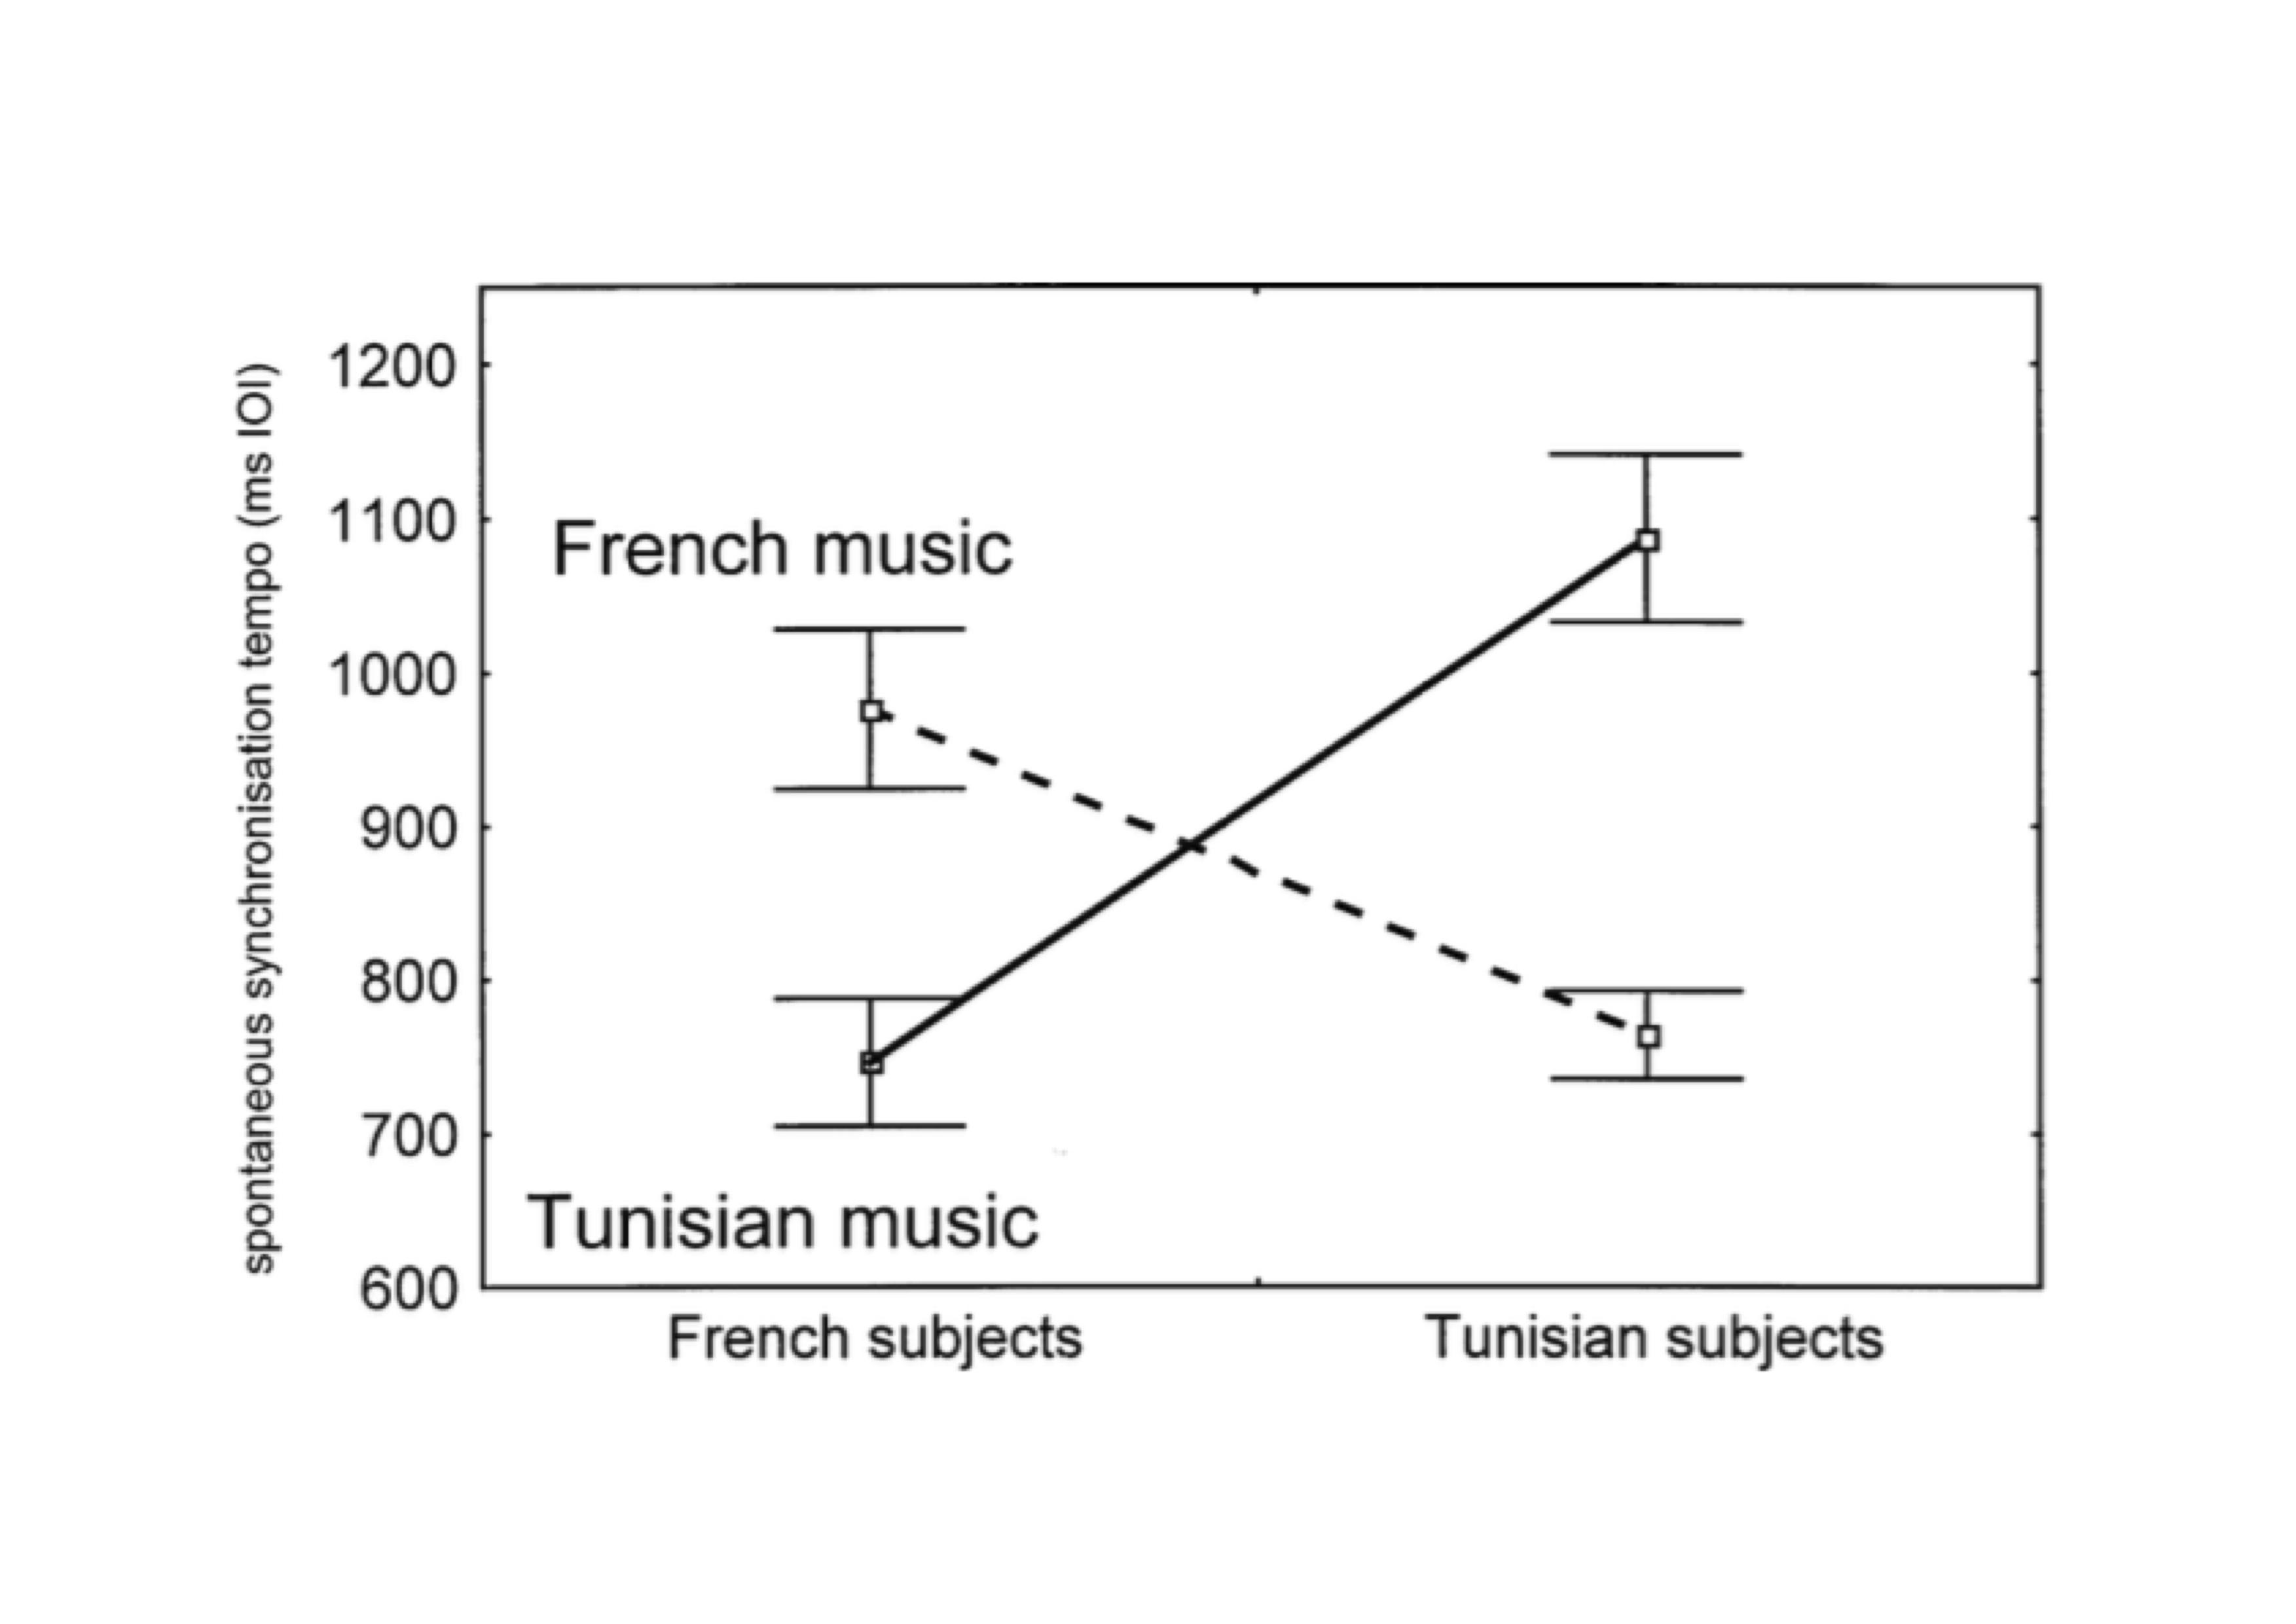
\includegraphics{figures/DrakeBenElHeni2003Fig2} 

}

\caption{Average time interval between taps (IOI, in ms) for two groups of listeners and two types of music (from Drake and Ben El Heni, 2003, Fig.2).}\label{fig:drakebenelheni2003fig2}
\end{figure}

\begin{quote}
These results show that there is no difference between both groups (French vs.~Tunisian listeners; both groups have the same IOI on average), and that there is also no difference between both types of music (French vs.~Tunisian music; both types of music result in the same IOI on average). Does this mean that the two independent variables have no effect at all? They absolutely do: it turned out that French listeners produced longer IOIs between taps when listening to French music, while, on the other hand, Tunisian listeners produced longer IOIs when listening to Tunisian music. Thus, all listeners produced longer IOIs when listening to a type of music they knew, and shorter IOIs when listening to a type of music they did not know. \citet{Drake03} conclude that listeners are better able to recognize and understand musical structure in music from their own musical culture compared to music from another culture. This pattern is a classic crossover interaction effect, in which one independent variable's effect is exactly opposite in the various conditions defined by the other independent variable.
\end{quote}

\begin{center}\rule{0.5\linewidth}{0.5pt}\end{center}

If it turns out that there is an interaction effect, we cannot sensibly interpret any main effects. This was already illustrated in example 6.5: we cannot conclude that there is no difference between the types of music. However, the size (and direction) of the difference depends on the other independent variable(s), in this case, group/nationality of listeners. Many studies are specifically aimed at demonstrating interaction effects: it is not main effects that are the topic of research, but their interaction, precisely as in example 6.5 above.

It is difficult to schematize a factorial research design, because it features multiple independent variables (with multiple levels each). We could schematically represent these by indexing the manipulation, which was previously shown simply as \texttt{X}. The first index (subscript) indicates the level for the first independent variable or factor, while the second index indicates the second factor's level. Following this system, we can schematize the design from example 6.5 as follows:

\begin{verbatim}
  R    X_{1,1}   O1
  R    X_{1,2}   O2
  R    X_{2,1}   O3
  R    X_{2,2}   O4
\end{verbatim}

Combining many factors into one big factorial design may often seem seductive: why not investigate how all these factors interact with one another? However, the most sensible option is not to do this, and, instead, limit the number of factors. Firstly, as we will see later, the number of observation has to keep up with the number of possible combinations of factors. Adding more factors means that many more participants (or other units) are needed. Secondly, it is more difficult to guarantee that all combinations of factors are perfectly comparable \citep[p.266]{SCC02}: may we reasonably compare Tunisian participants listening to Tunisian music in Tunisian with French participants listening to French music in France? The more combinations of factors are featured in the study, the trickier it becomes to ensure that these combinations are comparable. Thirdly, interactions are notoriously difficult to interpret, which also becomes trickier as interactions become more complex and span a greater number of factors. For all of these reasons, it is better to study the effects of multiple factors in separate individual studies \citep{Quene10}.

We will come back later to the analysis and interpretation of data from factorial experimental designs (Chapter \ref{ch:anova}).
In the meantime, we will concentrate on designs that have just one independent variable.

\hypertarget{sec:within-subject-designs}{%
\section{Within-subject designs}\label{sec:within-subject-designs}}

At the outset of the chapter, we spoke about manipulating an independent variable either between or within subjects (§\ref{sec:betweenwithinparticipants}). In most designs discussed above, a separate group was formed for each value of the independent variable(s); we call this a between subjects design. The independent variable's value differs between participants.

However, some independent variables may also be manipulated within participants. In such cases, we take repeated measures for (within) the same participants from the same group, switching out different conditions of the independent variable. In the example below, the independent variable, `language' (native or non-native), is varied within participants. We call this a within subjects design.

\begin{center}\rule{0.5\linewidth}{0.5pt}\end{center}

\begin{quote}
\emph{Example 6.6}: \citet{JGSH13} investigated the fluency of participants' speech in their native language (Turkish) and in a non-native language (Dutch). The participants first performed a number of speech production tasks in their native language, a few weeks after which they did the same for Dutch. One of the dependent variables was the number of filled pauses (e.g., \emph{uh, uhm}) per second of speech: the greater the prevalence of pauses, the lesser the degree of fluency. As we might expect, the speakers did turn out to produce more pauses (i.e., speak less fluently) in the non-native language compared to their native language. However, one of the goals of this study was to investigate to which extent we may trace back individual fluency differences in the non-native language to individual fluency differences in the native language. These two measurements turned out to be highly correlated (\(r = 0.73\); see Chapter \ref{ch:correlation-regression} for more on this). Speakers that have many pauses in the non-native language also have many pauses in their native language. The researchers argue that we must take this correlation into account when teaching and testing speaking ability in a non-native language.
\end{quote}

\begin{center}\rule{0.5\linewidth}{0.5pt}\end{center}

The research design described here can be schematized as follows:

\begin{verbatim}
   X1   O1   X2   O2
\end{verbatim}

Despite the many threats it poses to internal validity (including history, maturation, guiding influence of pretests), such a design is often useful. In the example above, it is essential that it is the \emph{same} participants that carry out speaking tasks in both languages (conditions) -- no other method will be adequate for answering the research questions.

\hypertarget{designing-a-study}{%
\section{Designing a study}\label{designing-a-study}}

A researcher who intends to carry out a study has to settle on a way of collecting data: they have to choose a particular design for their study. Sometimes, a standard designed may be chosen, for instance, one of the designs discussed above. In other cases, the researcher will have to devise their own design. Naturally, the design chosen should fit well with the research question \citep{Levin99}, and it should exclude as many disruptive, potentially validity-threatening variables as possible. Designing a study is a skill that researchers hone with practice. In the example below, we will try to show to you which reasoning and arguments play a role in developing a design for a study.

Suppose that we would like to investigate whether the way in which test questions are asked, as open vs.~closed questions, influences students' scores on the relevant test. If we use a simple design, we will first administer a test with open questions to a group of respondents, and then, a comparable test with closed questions to the same respondents. If the resulting scores are sufficiently correlated, we conclude that both tests measure the same thing, and that performance on the test is not significantly influenced by the way questions are asked. This design can be schematized as follows:

\begin{verbatim}
   Open   O1   Closed   O2
\end{verbatim}

However, this research design does have various weaknesses. Firstly, it is not prudent to first administer all open question tests at the first time point, and leave all closed question tests for the second time point. This is because performance on the second test will always be influenced by effects of ordering (transfer effects): respondents remember and, thus, learn something from the first measurement. However, this transfer always works in one direction, which means that we expect relatively higher performance on the test with closed questions (at the second time point). Because of this, it is better to randomly distribute the open question and close question tests between the first and second time point.

Secondly, all respondents might have been influenced by any events that took place between the two time points (history), for instance, by some instruction relevant to the test's subject matter. Because there is no control group, we cannot take this type of effect into account.

A third problem lies in the way in which the reasoning from findings to conclusions is constructed. For the current example, we defined this reasoning as follows: if scores on both tests are sufficiently correlated, both tests measure the same thing. If you stop and think about it, you might agree with us that this is a strange bit of reasoning. The underlying research question really seems to be whether the correlation between performance on different tests with different types of questions is the same as the correlation between performance on different tests with the same types of questions, since we do assume that the latter group of tests measure the same thing. This, in itself, defines a control group: respondents who, at both points in time, write tests with the same types of questions. Just to be sure, let us add not one, but two control groups: one with open questions at both time points, and one with closed questions at both time points.

By doing this, we have improved the design in at least two ways: (1) tests are randomized between times of measurement, and (2) relevant control groups have been added. At this point, we may schematize our design as follows:

\begin{verbatim}
       Exp. group 1       Open    O1   Closed   O2
       Exp. group 2      Closed   O3    Open    O4
      Control group 1     Open    O5    Open    O6
      Control group 2    Closed   O7   Closed   O8
\end{verbatim}

For all four groups, we may now determine the correlation between their performance at the first and the second time point. We can subsequently compare these correlation results between the four groups, and use this to answer the research question. This example shows us that the conclusions that can be draw from research results are directly dependent on the design that was chosen \citep{Levin99}. In the first design, a low correlation would lead to a conclusion that the two types of testing investigated do \emph{not} test for the same intellectual skills in our respondents. However, in the second design, the same low correlation in the first group (experimental group 1) does not have to lead to the same conclusion! This is because the conclusion also depends on the degree of correlation that was found in the other groups.

\hypertarget{in-conclusion}{%
\section{In conclusion}\label{in-conclusion}}

Despite all the books, manuals, websites, and other instructional materials that are available, it is still much too often that we encounter studies with methodological problems in their research questions, operationalization, design, drawing of samples, and/or data collection. Not only do these problems cause a waste of time, money, and energy, but they also yield knowledge that is less reliable, valid, and robust than would otherwise have been possible. The following checklist for good research practice (partly taken from \url{https://www.linkedin.com/groups/4292855/4292855-6093149378770464768}) may preempt many problems during a study's later stages.

\begin{enumerate}
\def\labelenumi{\arabic{enumi}.}
\item
  Give your research questions plenty of thought, and formulate them fully into the smallest detail. If the questions have not been formulated clearly, or if there are many sub-questions, keep working on the questions.
\item
  Arrange the research questions according to their priority. This will help in making good choices regarding design, sampling, operationalization, etc.
\item
  Think long and hard about your study's design. According to an informal rule of thumb, each hour spent thinking about your study's design will save you 10 hours of additional data analysis and interpretation in the future. Put differently: spending an hour less on thinking about your design will cost you 10 hours of work down the road.
\item
  Think of various alternative designs for your study, and think about each possible design option's advantages and disadvantages.
\item
  Imagine the future: you have completed your research project, analysed your data, and written your report or thesis. Which message would you like to impart upon the readers of your report? How does your study's design contribute to this message? What might you change in your design to make this message even clearer? Think of the direction you would like to take, not just of where you are now.
\item
  Write a research plan in which you describe the various methodological aspects of your study. Explain the details of and the reasoning behind your research questions, design, sample, method of measurement, data collection, instruments of measurement (e.g., questionnaire, software), other requirements (e.g., laboratory environment, transportation), and statistical processing. You will be able to reuse parts of this research plan in your report. When writing your plan, make sure to include a schedule: when will which milestone be reached?
\item
  Write out what statistical analyses you will use on your data before your actually start collecting any data. Again, be as explicit as possible (using a script, step-by-step plan, or similar). Make up a miniature collection of fake observations, or real observations from the pilot phase of your study, and analyse these data as if this were your definitive collection of data. Make adjustments to your research plan as needed.
\item
  Once you are collecting data, do \emph{not} make any changes to your research plan. Keep to this plan and the schedule you made. Analyse your data in the way specified in the (previously adjusted) research plan. Do discuss in your report any problems that arose during the study. If serious problems occur, halt your project, and consider starting anew with an improved version of your study.
\end{enumerate}

\hypertarget{ch:samples}{%
\chapter{Samples}\label{ch:samples}}

In generalizing the outcome of a study to the population or the sample, the quality of the sample is all-important. Does the sample adequately reflect the population? To give an extreme example of this: if a sample consists of girls in the last year of primary education, we cannot properly generalize the results to the population of students in primary education, because the sample does not form a good reflection of this population (which consists of boys and girls in all years of the curriculum).

Depending on the method used by the researchers to select participants, many kinds of samples may be distinguished. In this chapter, we make a rough distinction between: (1) convenience samples, (2) systematically drawn samples, and (3) samples drawn at random. For further discussion of the way in which samples may be drawn and the problems that play a role in this, we refer the reader to standard reference works on this topic \citep{Coch77, Thom12}.

\hypertarget{sec:convenience-samples}{%
\section{Convenience samples}\label{sec:convenience-samples}}

Work in the social sciences often uses samples that happen to present themselves to the researcher, so-called \emph{convenience samples}. The researcher carries out the experiment with individuals that happen to be available to them more or less by chance. Some studies use paid or unpaid volunteers. In other studies, students are recruited, who are required to log some number of hours as participants as a part of their studies, or, sometimes, a colleague of the researcher"s sends their own students to participate in the study. A sample of this kind is not without its dangers. The researcher has no control whatsoever over the degree to which results can be generalized to the population. Of course, the researcher does have a population in mind, and will exclude participants that do not form a part of the intended population (such as non-native speakers) from the study, but the researcher cannot say anything about how representative the sample is.

It is especially in psychology that this convenience sampling has led to heated discussion. For instance, a survey showed that 67\% of samples used in published studies in psychology performed in the US was exclusively composed of undergraduate students enrolled in Psychology courses at American universities \citep{Henr10}. Naturally, samples like this are hardly representative. As a consequence, the theories based on these data have but a limited scope: they are likely to apply predominantly to the type of individuals (first world, young, highly educated, white) that are also highly represented in the samples \citep{Henr10}. Research in linguistics often also uses a convenience sample. Children that participate as participants often have highly educated parents (who often tend to have a linguistics background themselves, which likely means that they have above-average verbal skills), and adult participants are often students from the researchers' environment, who, therefore, also have above-average levels of education and verbal skill.

Despite the valid objections raised against this type of sample, practical considerations often force researchers to use a convenience sample that presents itself. In such cases, we recommend keeping track of the extent to which this convenience sample distinguishes itself from the population over which the researcher would like to generalize. To conclude this discussion of samples that present themselves naturally, we provide an example of the dangers this type of sample carries.

\begin{center}\rule{0.5\linewidth}{0.5pt}\end{center}

\begin{quote}
\emph{Example 7.1}: Some years ago, there was a televised contest in which nine candidates competed on their singing skills. Viewers were invited to announce their preference by phone. For each of the nine candidates, a separate phone line had been opened. For each call, the corresponding candidate received one point. The person with the greatest number of points within a set time limit would win. The audience's response was overwhelming: large swaths of the Dutch phone network were over capacity. Very soon, one of the candidates turned out to have a considerable lead over the others. However, in the course of the evening, this lead became smaller and smaller. In the end, there was only a few calls' difference between the top two candidates. It was striking to see that, as the evening progressed, the relative differences between participants gradually diminished.
\end{quote}

\begin{center}\rule{0.5\linewidth}{0.5pt}\end{center}

We may see this voting procedure as drawing a sample of callers or voters. However, this sample is far from representative. If many voters would like to vote for the same candidate, the phone line dedicated to this candidate will reach and exceed its capacity. This means that singers who drew many callers will receive relatively fewer votes than singers who draw few callers, because the latter singers' phone lines will not be over capacity. It is precisely for the most popular candidates that a voter is most likely to be unable to cast their vote. Because of this, the real difference in the number of calls per candidate will be far greater than what the organizers measured. The organizers themselved caused this systematic distortion of the results (bias) by opening a separate phone line for each of the nine candidates. The data could have been much more representative if the organizers had opened nine phone lines accessible through one single phone number. In such a scenario, the sample of callers who were able to cast their vote would have been representative for the population of all callers, which was not the case in reality.

\hypertarget{sec:systematic-samples}{%
\section{Systematic samples}\label{sec:systematic-samples}}

When the elements in the \emph{sampling space} (i.e., the set of possible elements in a sample) are systematically ordered in some way, a reasonably representative sample can be obtained using a \emph{systematic sampling procedure}. Ordering may, for instance, involve a list of names.

\begin{center}\rule{0.5\linewidth}{0.5pt}\end{center}

\begin{quote}
\emph{Example 7.2}: Let us assume for the moment that we would like to make study of language ability in students in the third year of secondary education. However, the entire population of third year students is far too great to measure all third year students' language ability (reading, writing, speaking, and listening): this group contains about 200,000 students. Consequently, we need to draw a sample. The Dutch Ministry of Education, Culture, and Science has a system in which a list of all schools with third year students is included. An obvious way of proceeding would be to take this list and include each 100th school on the list into the sample. This procedure will presumably result in a reasonably representative sample.
\end{quote}

\begin{center}\rule{0.5\linewidth}{0.5pt}\end{center}

However, two factors may muddle the waters in drawing such a systematic sample, the first of which is the \emph{response rate}. If a considerable proportion of schools that were contacted do not cooperate, we are actually dealing with self-selection (see §\ref{sec:internalvalidity} point 5) and, thus, with a convenience sample that presents itself (see §\ref{sec:convenience-samples}). This is an unwanted situation, since the schools that did cooperate presumably have a greater `sense of duty' than the schools that refused participation or than the average school. Moreover, students in the responding and non-responding schools may differ from one another (see §\ref{sec:internalvalidity} point 5). This means that the eventual sample may perhaps be no longer representative of the population of all third year students. This, in turn, has as a consequence that the results measured cannot be properly generalized to other third year students at other schools.

The second factor that may influence whether a systematic sample is representative is the presence of a \emph{disruptive trend effect}. We speak of a disruptive trend effect when elements of the population have a greater chance of ending up in the sample if they have a certain characteristic, compared to population elements that do not have this characteristic. In our example of measuring language ability in third year students, we are dealing with a disruptive trend effect. This is because not all students have an equal chance of being in the sample. After all, it is each individual \emph{school} (not: each individual student) that has an equal chance of being in the sample. The consequence of this is that the sample will contain relatively many third year students from small schools with relatively few students, while, conversely, there will be relatively few third year students from large schools with relatively many students. Thus, third year students from large schools will be underrepresented. Is this a bad thing? It might be, because language ability (dependent variable) is partially influenced by the type of instruction, and type of instruction is influenced by the size of a school. This means that the sample described above is not representative for the population of third year students. Once again, this means that the results measured cannot be properly generalized to other third year students at other schools.

\hypertarget{sec:random-samples}{%
\section{Random samples}\label{sec:random-samples}}

The disruptive trend effect described above can be avoided by \emph{random sampling}. Random sampling may happen in various ways, of which we will discuss three.

The first type is simple random sampling: in this procedure, all elements of the population have an equal chance of being drawn. This may, for instance, be realized by giving all elements a \emph{random} number and, depending on the size of the sample, selecting each \(n\)-th element. For choosing random numbers, researchers can make use of tables of random numbers (see Appendix \ref{app:randomnumbers}). Random numbers can also be generated by calculators, computers, spreadsheet programs, etc. (Using this type of random numbers is advisable, since a ``random'' order created by humans is not truly random.) However, one condition for applying this method is that the elements of the population (sampling space) are registered in advance, so that they may all be given numbers in some way.

\begin{center}\rule{0.5\linewidth}{0.5pt}\end{center}

\begin{quote}
\emph{Example 7.3}: We would like to draw a sample of n = 400 primary schools, which is about 4\% of the population of primary schools in the Netherlands. To do this, we request from the Dutch Ministry of Education, Culture, and Science a list of all 9,000 primary schools; this list is the sampling space. After this, we number all schools with subsequent numbers \((1, 2, 3 \ldots, 9000)\). Finally, we select all primary schools whose number happen to end in 36, 43, 59, or 70 (see Appendix \ref{app:randomnumbers}, first column, last two digits). Using this procedure, we randomly select 4 of 100 possible last-two-digit combinations, or 4\% of all schools.
\end{quote}

\begin{center}\rule{0.5\linewidth}{0.5pt}\end{center}

The second type of random sampling is \emph{stratified random sampling}. We are dealing with this type of sampling when we know the value of a particular characteristic (e.g., religious denomination) for each element of the population, and we make sure that elements within the sample are divided equally according to this characteristic. To do this, we divide the sample into so-called `strata' or layers (Lat. \emph{stratum}, `cover, layer,' related to English \emph{street}, originally meaning `paved road'). Let us return to our primary school example to clarify a few things. Suppose that, for whatever reason, we are now interested in making the sample (still 4\% of the population of primary schools) such that public, catholic, and protestant schools are represented in equal amounts. We therefore devise three lists, a separate one for each type of school. Within each list, we proceed just like for simple random sampling. Eventually, our three sub-samples from the three strata are combined.

\emph{Quota sampling} goes one step further compared to stratified random sampling: we now also take advantage of the fact that we know the distribution of a certain characteristic (e.g., denomination) within the population. From the list of primary schools, we might have gleaned that 35\% of schools is public, 31\% is catholic, 31\% is protestant, and 3\% has some other denomination. From this sampling space, we now draw multiple `stratified' random samples such that the proportion of schools in each stratum correctly reflects the proportions of this characteristic in the sampling space \((35 : 31 : 31 : 3)\).

\hypertarget{spss}{%
\subsection{SPSS}\label{spss}}

In order to create a column containing random numbers;

\begin{verbatim}
Transform > Compute...
\end{verbatim}

Select an existing variable (drag to Variables panel) or enter the name of a new variable.
From the panel ``Function Group'', choose ``Random numbers'', and choose \texttt{RV.UNIFORM}.
This function samples \textbf{r}andom \textbf{v}alues from a flat or \textbf{uniform} probability distribution, meaning that each number between the lower and upper limit has an equal chance of being sampled.
Enter \texttt{0} as lower limit and \texttt{9999} as upper limit, or use other limits as appropriate.
Confirm with \texttt{OK}.
This results in a (new or overwritten existing) column with random numbers.

If you wish to sample random numbers from a normal density distribution (see §\ref{sec:normaldistribution}), then use the function \texttt{RV.NORMAL(mean,stdev)}.

We may provide a starting value for the random number generator, in order to make reproducible analyses (and examples):

\begin{verbatim}
Transform > Random Number Generators...
\end{verbatim}

In the panel ``Active Generator Initialization'', check the option \texttt{Set\ Starting\ Point}, and enter a starting value, such as your favourite number. Confirm with \texttt{OK}.

You can use the resulting random numbers for randomly selecting units (e.g.~participants, stimuli) for a sample, and also to randomly assign the selected units to conditions, treatments, groups, etc.

\hypertarget{r}{%
\subsection{R}\label{r}}

In R we may generate random numbers using the predefined function \texttt{runif}.
This function samples \textbf{r}andom values from a flat or \textbf{unif}orm probability distribution, meaning that each number between the lower and upper limit has an equal chance of being sampled. The default limits are \((0,1)\). You may round off the resulting random values to integer numbers, as was done in Appendix \ref{app:randomnumbers}.

If you wish to sample random numbers from a normal density distribution (see §\ref{sec:normaldistribution}), then use the function \texttt{rnorm(n,mean,sd)}.

We may provide a starting value (called a ``seed'') for the random number generator, in order to make reproducible analyses (and examples), using the predefined function \texttt{set.seed}:

\begin{Shaded}
\begin{Highlighting}[]
\KeywordTok{set.seed}\NormalTok{(}\DecValTok{20200912}\NormalTok{) }\CommentTok{\# reproducible example, number is date on which this chunk was added}
\KeywordTok{round}\NormalTok{ ( }\KeywordTok{runif}\NormalTok{( }\DataTypeTok{n=}\DecValTok{5}\NormalTok{, }\DataTypeTok{min=}\DecValTok{0}\NormalTok{, }\DataTypeTok{max=}\DecValTok{9999}\NormalTok{ ) ) }\CommentTok{\# similar to Appendix A}
\end{Highlighting}
\end{Shaded}

\begin{verbatim}
## [1] 8193 7482 4206 1684 5653
\end{verbatim}

You can use the resulting random numbers for randomly selecting units (e.g.~participants, stimuli) for a sample, and also to randomly assign the selected units to conditions, treatments, groups, etc.

\hypertarget{sec:sample-size}{%
\section{Sample size}\label{sec:sample-size}}

When you read various research articles, one of the first things that catches the eye is the enormous variation in the number of respondents. In some studies, several thousands of participants are involved, while others only have several multiples of 10, or even fewer. Here, we will discuss two aspects that influence the required size of one's sample: the population's relative homogeneity, and the type of sampling. In the chapters that follow, we will discuss two more aspects that influence the desired sample size: the desired precision (effect size, §\ref{sec:ttest-effectsize}) and the desired likelihood to demonstrate an effect if it is present in the population (power, §\ref{sec:effectsize-power}).

\begin{center}\rule{0.5\linewidth}{0.5pt}\end{center}

\begin{quote}
\emph{Example 7.4}: When cars are tested (for magazines or television), only one car of each type is tested. The results of this tested token are generalized without reservation to all cars of the same type and make. This is possible because the population of cars to which generalization is made is especially homogenous, since the manufacturer strives to make the various tokens of a car type they sell maximally identical.
\end{quote}

\begin{center}\rule{0.5\linewidth}{0.5pt}\end{center}

Firstly, the required sample size depends on the population's homogeneity. If a population is \emph{homogeneous}, like the cars in example 7.4, a small sample will suffice. Things are different when, for instance, we would like to analyse conversation patterns in pre-schoolers. When looking at pre-schoolers' conversation patterns, we come across great differences; conversation patterns exhibit a very high degree of variation. (Some children speak in full sentences, others mainly remain silent. Moreover, there are great individual differences in children's linguistic development.) This means that, to obtain a reasonable picture of language development in pre-schoolers, we need a much bigger sample. Thus, the required sample size increases as the population to which we would like to generalize is less homogeneous (more heterogeneous).

Secondly, the required sample size also depends on the nature of the sample. If a population contains clear strata, but -- for whatever reason -- we do not apply stratified or quota sampling, then we will need a larger sample compared to a situation where we had, indeed, applied one of these two methods. This is because, in these two latter methods, the researcher actively ensures that strata are represented in the sample either to equal extents, or according to the correct proportions; in simple random sampling, this is left to chance. We must then appeal to the ``law of large numbers'' to make sure that a sufficient number of elements from each stratum makes its way into the sample, in order to justify generalization of the results to these various strata. Obviously, this law only works with a sufficiently large sample. When the sample is small, we can in no way be sure that the various strata are represented in the sample to a sufficient extent.

Returning to our primary school example, if we selected three primary schools according to simple random sampling, the chance that this would lead to exactly one public, one catholic, and one protestant school is, no doubt, present. However, other outcomes are quite likely, as well, and even much more likely. If we use stratified or quota sampling, we are guaranteed to have one element (school) of each denomination in our sample. This improves our grounds for generalization, and strengthens external validity.

After all these recommendations that are worth taking to heart, it is now time to discuss how we can describe and analyse research data to properly answer our research questions. This will be done in the next part of this book.

\hypertarget{part-part-ii-descriptive-statistics}{%
\part*{Part II: Descriptive statistics}\label{part-part-ii-descriptive-statistics}}
\addcontentsline{toc}{part}{Part II: Descriptive statistics}

\hypertarget{ch:frequencies}{%
\chapter{Frequencies}\label{ch:frequencies}}

\hypertarget{introduction-3}{%
\section{Introduction}\label{introduction-3}}

When analysing data, a distinction is often made between
qualitative and quantitative methods. With the first method,
observations (e.g.~answers in interviews) are represented in
words, and with the second method, observations (e.g.~speech
pauses in interviews) are represented in numbers. In our opinion,
the difference between qualitative and quantitative methods
lies in how observations are represented, and
how arguments are made on the basis of these observations.
Sometimes it is also possible to analyse the very same data (e.g.~
interviews) both qualitatively and quantitatively. The major
advantages of quantitative methods are that the data can be summarised
relatively straightforwardly (this is the subject of this part of the
syllabus), and that it is relatively simple to draw meaningful conclusions
on the basis of the observations.

\hypertarget{sec:frequencies}{%
\section{Frequencies}\label{sec:frequencies}}

Quantitative data can be reported in various different ways.
The most straightforward way would be to report the raw data, preferably
sorted according to the observed variable's value.
The disadvantage of this is that a potential pattern in the observations
will not be easily visible.

\begin{center}\rule{0.5\linewidth}{0.5pt}\end{center}

\begin{quote}
\emph{Example 8.1}: Students \((N=50)\) in a first year
course reported the following values for their shoe size, a
variable of an interval level of measurement:\\
36, 36, 37, 37, 37, 37, 37, 37, 38, 38, 38, 38, 38, 38, 39, 39, 39, 39,
39, 39, 39, 39, 39, 39, 39, 39, 39, 39, 39, 39, 39, 39, 39, 40, 40, 40,
40, 40, 40, 41, 41, 41, 41, 41, 42, 42, 43, 43, 44, ??.\\
One of the students did not provide an answer; this missing answer is
shown here as ??.
\end{quote}

\begin{center}\rule{0.5\linewidth}{0.5pt}\end{center}

It is usually more insightful and efficient to summarise observations
and report them in the form of a \emph{frequency} for each value.
This frequency indicates the \emph{number} of observations which have a certain value,
or which have a value in a certain interval or class. In order to get
the frequencies, we thus \emph{count} the number of observations with a certain
value, or the number of observations in a certain interval. These
frequencies are reported in a table. We call such a table a
frequency distribution.

As a first example, Table \ref{tab:klankfreq} provides a
frequency distribution of a discrete variable of \emph{nominal} level of measurement,
namely the phonological class of sounds in Dutch \citep{LKCG07}.
\#52-56

\begin{table}

\caption{\label{tab:klankfreq}Frequency distribution 
              of the phonological class of speech sounds
              in the *Corpus of Spoken Dutch* 
              (C=consonant, V=vowel; lang=long vowel, kort=short vowel).}
\centering
\begin{tabular}[t]{llr}
\toprule
main.class & sub.class & count\\
\midrule
C & plos & 585999\\
C & fric & 426097\\
C & liq & 249275\\
C & nas & 361742\\
C & glide & 146344\\
\addlinespace
V & lang & 365887\\
V & kort & 428832\\
V & schwa & 341260\\
V & diph & 61638\\
V & rest & 1146\\
\bottomrule
\end{tabular}
\end{table}

As a second example, Table \ref{tab:shoesize} provides a
frequency distribution of a continuous variable of \emph{interval}
level of measurement, namely the aforementioned shoe size
of first year students (Example 8.1).

\begin{longtable}[]{@{}lcccccccccc@{}}
\caption{\label{tab:shoesize} Frequency distribution of the self-reported shoe sizes of \(N=50\) students in a first year course (see Example 8.1 above).}\tabularnewline
\toprule
\endhead
Shoe size & 36 & 37 & 38 & 39 & 40 & 41 & 42 & 43 & 44 & ??\tabularnewline
Number & 2 & 6 & 6 & 19 & 6 & 5 & 2 & 2 & 1 & 1\tabularnewline
\bottomrule
\end{longtable}

Nevertheless, when a numerical variable is able to assume a great many different
values, the frequency distribution thus consequently becomes large and confusing.
We then add together values in a certain interval,
and afterwards make a frequency distribution on the smaller number
of intervals or classes.

\begin{center}\rule{0.5\linewidth}{0.5pt}\end{center}

\begin{quote}
\emph{Example 8.2}: When Queen Beatrix of the Netherlands was giving her last Queen's Speech,
on 18th September 2012, she paused some \(305\times\). The frequency distribution
of the pause length (measured in seconds) is shown in
Table \ref{tab:queensspeech2012pauses}.
\end{quote}

\begin{center}\rule{0.5\linewidth}{0.5pt}\end{center}

\begin{longtable}[]{@{}cr@{}}
\caption{\label{tab:queensspeech2012pauses} Frequency distribution of the length of speech pauses (seconds)
in the Queen's Speech of 18th September 2012, given by Queen Beatrix of the Netherlands
\((N=305)\).}\tabularnewline
\toprule
Interval & Number\tabularnewline
\midrule
\endfirsthead
\toprule
Interval & Number\tabularnewline
\midrule
\endhead
4.50--4.99 & 1\tabularnewline
4.00--4.49 & 0\tabularnewline
3.50--3.99 & 2\tabularnewline
3.00--3.49 & 7\tabularnewline
2.50--2.99 & 4\tabularnewline
2.00--2.49 & 25\tabularnewline
1.50--1.99 & 32\tabularnewline
1.00--1.49 & 16\tabularnewline
0.50--0.99 & 67\tabularnewline
0.00--0.49 & 151\tabularnewline
\bottomrule
\end{longtable}

\hypertarget{sec:intervals}{%
\subsection{Intervals}\label{sec:intervals}}

For a variable of nominal and ordinal level of measurement, we generally
use the original categories to make the frequency distribution
(see Table \ref{tab:klankfreq}), although it is possible to add categories
together. For a variable of interval or ratio level of measurement, a
researcher can choose the number of intervals in the frequency distribution
themself. Sometimes that is not necessary, for instance because the variable has
a clear number of different discrete values (see Table \ref{tab:shoesize}).
However, sometimes, as a researcher you have to decide for yourself how many
intervals you should distinguish, and how to determine the
interval boundaries (see Table \ref{tab:queensspeech2012pauses}).
In this instance, the following are recommended \citep[Ch.2]{Ferg89}:

\begin{itemize}
\item
  Ensure that all observations (i.e.~the entire range) fall into
  roughly 10 to 20 intervals.
\item
  Ensure that all intervals are equally wide.
\item
  Make the lower limit of the first or second interval the same as
  the width of the intervals (see
  Table \ref{tab:queensspeech2012pauses}: every interval is 0.50 s
  wide, and the second interval's lower limit is also 0.50).
\item
  Order the intervals in a frequency distribution from bottom
  to top in increasing order (i.e.~from top to bottom in
  descending order), see
  Table \ref{tab:troonrede2012pauzes}).
\end{itemize}

The wider we make the intervals, the more information we lose
about the precise distribution within each interval.

\hypertarget{spss-1}{%
\subsection{SPSS}\label{spss-1}}

\begin{verbatim}
Analyze > Descriptive Statistics > Frequencies...
\end{verbatim}

Select variable (drag to the ``Variable(s)'' panel).\\
Tick: \texttt{Display\ frequency\ tables}.\\
Choose \texttt{Format}, choose: \texttt{Order\ by:\ Descending\ values}.\\
Confirm with \texttt{OK}.\\

\hypertarget{r-1}{%
\subsection{R}\label{r-1}}

\begin{Shaded}
\begin{Highlighting}[]
\NormalTok{enq2011 \textless{}{-}}\StringTok{ }\KeywordTok{read.table}\NormalTok{( }
    \DataTypeTok{file=}\KeywordTok{url}\NormalTok{(}\StringTok{"http://www.hugoquene.nl/R/enq2011.txt"}\NormalTok{), }
    \DataTypeTok{header=}\OtherTok{TRUE}\NormalTok{ )}
\KeywordTok{table}\NormalTok{( enq2011}\OperatorTok{$}\NormalTok{shoe, }\DataTypeTok{useNA=}\StringTok{"ifany"}\NormalTok{ ) }
\end{Highlighting}
\end{Shaded}

The output of the above \texttt{table} command is shown in Table \ref{tab:shoesize}.
The code \texttt{NA} (Not Available) is used in R to indicate missing data.

\begin{Shaded}
\begin{Highlighting}[]
\KeywordTok{table}\NormalTok{( }\KeywordTok{cut}\NormalTok{( troon2012, }\DataTypeTok{breaks=}\KeywordTok{seq}\NormalTok{(}\DataTypeTok{from=}\DecValTok{0}\NormalTok{,}\DataTypeTok{to=}\DecValTok{5}\NormalTok{,}\DataTypeTok{by=}\FloatTok{0.5}\NormalTok{) ) )}
\end{Highlighting}
\end{Shaded}

Parse this task from the innermost brackets outwards:
(i) \texttt{seq}: make a sequence from 0 to 5 (units, here: seconds) in increments of 0.5 seconds,
(ii) \texttt{cut}: cut up the dependent variable \texttt{length} in intervals based on this sequence,
(iii) \texttt{table}: make a frequency distribution of these intervals.

This task's output is shown (in edited form) in Table \ref{tab:queensspeech2012pauses}.

\hypertarget{sec:barcharts}{%
\section{Bar charts}\label{sec:barcharts}}

A bar chart is the graphical representation of the
frequency distribution of a discrete, categorical variable (of
nominal or ordinal level of measurement). A bar chart is constructed
of rectangles. All rectangles are equally wide, and the
rectangle's height corresponds with the frequency of that category. The
surface area of each rectangle thus also corresponds with that category's frequency.
In contrast to a histogram, the rectangles are \emph{not}
joined up to each other along the horizontal axis, to
show that we are dealing with discrete categories.

\begin{figure}
\centering
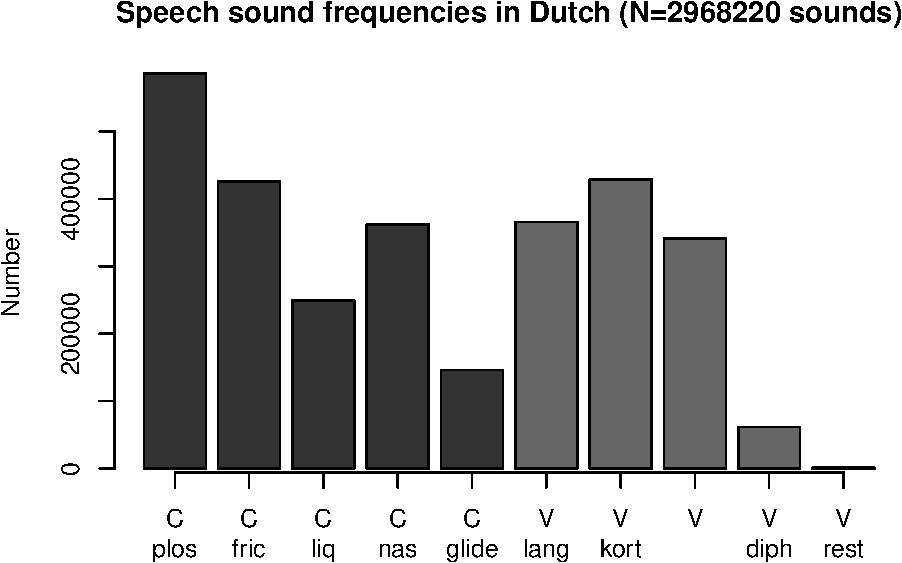
\includegraphics{QMS-EN_files/figure-latex/klankfreq-barplot-1.pdf}
\caption{\label{fig:klankfreq-barplot}Bar chart of the frequency distribution of phonological class of speech sounds in the Corpus of Spoken Dutch (C=consonant, V=vowel).}
\end{figure}

A bar chart helps us to determine at a glance the most important
distributional characteristics of a discrete variable:
the most characteristic (most frequently occurring) value, and the
distribution across categories. For the sound frequencies
in Dutch (Figure \ref{fig:klankfreq-barplot}), we
see that amongst the consonants the plosives
occur the most, that amongst the vowels the
short vowels occur the most, that diphthongs
are not used much (the sounds in Dutch \emph{ei, ui, au}), and that
more consonants are used compared with vowels.

Tip: Avoid shading and other 3D-effects in a bar chart! These make
the width and height of a rectangle less readable, and
the visible surface area of a shaded rectangle or
of a bar no longer corresponds well with the frequency.

\hypertarget{sec:histograms}{%
\section{Histograms}\label{sec:histograms}}

A histogram is the graphical representation of a frequency distribution of
a continuous, numerical variable (of interval or ratio level of measurement).
A histogram is constructed of rectangles. The width of each
rectangle corresponds with the interval width (a rectangle can
also be one unit wide) and the height corresponds with the frequency
of that interval or value. The surface area of each rectangle
therefore corresponds with the frequency. In contrast to a
bar chart, the rectangles do join up to each other
along the horizontal axis.

\begin{figure}
\centering
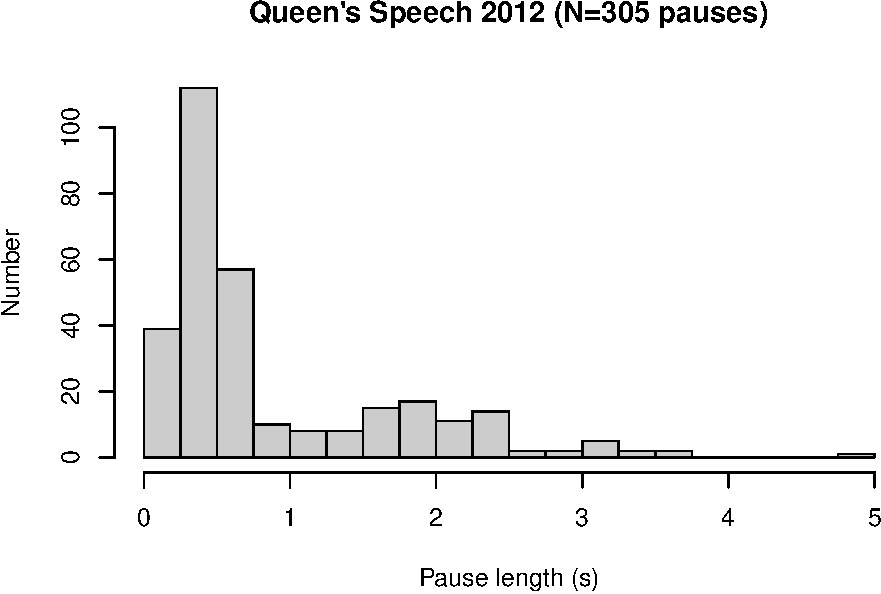
\includegraphics{QMS-EN_files/figure-latex/troonrede2012-hist-1.pdf}
\caption{\label{fig:troonrede2012-hist}Histogram for the lengths of pauses (in seconds) in the Queen's Speech of 18 September 2012, read by Queen Beatrix (N=305).}
\end{figure}

A histogram helps up to determine at a glance the most important distributional characteristics
of a continuous variable: the most characteristic
(most frequently occurring) value, the degree of dispersion, the
number of peaks in the frequency distribution, the position of the peaks,
and potential outliers.
(see §\ref{sec:outliers}).
For the pauses in the Queen's Speech of 2012
(Figure \ref{fig:troonrede2012-hist}), we see that the majority of pauses
last between 0.25 and 0.75 s (these are presumably pauses for breath),
that there are two peaks in the distribution (the second peak is at 2 s),
and that there is one extremely long pause (with a duration
of almost 5 s).

Tip: Avoid shading and other 3D-effects in a histogram! These
make the width and height of a rectangle less readable,
and the visible surface area of a shaded rectangle or of a bar
no longer correspond well with the frequency.

\hypertarget{spss-2}{%
\subsection{SPSS}\label{spss-2}}

\begin{verbatim}
Analyze > Descriptive Statistics > Frequencies...
\end{verbatim}

Select variable (drag to the ``Variable(s)'' panel).\\
Choose \texttt{Charts}, then pick \texttt{Chart\ type:\ Bar\ chart} for a
bar chart or \texttt{Chart\ type:\ Histogram} for a histogram (see
the above text for the difference between these options).\\
Confirm with \texttt{OK}.\\

\hypertarget{r-2}{%
\subsection{R}\label{r-2}}

You can make a bar chart like Figure \ref{fig:klankfreq-barplot} in R with the
following commands:

\begin{Shaded}
\begin{Highlighting}[]
\CommentTok{\# read data}
\NormalTok{klankfreq \textless{}{-}}\StringTok{ }\KeywordTok{read.table}\NormalTok{( }\DataTypeTok{file=}\StringTok{"data/klankfreq.txt"}\NormalTok{, }\DataTypeTok{header=}\NormalTok{T )}
\CommentTok{\# 20201130 column names in English}
\KeywordTok{dimnames}\NormalTok{(klankfreq)[[}\DecValTok{2}\NormalTok{]] \textless{}{-}}\StringTok{ }\KeywordTok{c}\NormalTok{(}\StringTok{"main.class"}\NormalTok{,}\StringTok{"sub.class"}\NormalTok{,}\StringTok{"count"}\NormalTok{)}
\CommentTok{\# make barplot from column \textasciigrave{}count\textasciigrave{} in dataset \textasciigrave{}klankfreq\textasciigrave{}}
\KeywordTok{with}\NormalTok{( klankfreq, }\KeywordTok{barplot}\NormalTok{( count, }\DataTypeTok{beside=}\NormalTok{T, }
                          \DataTypeTok{ylab=}\StringTok{"Frequency"}\NormalTok{,}
                          \DataTypeTok{main=}\StringTok{"Frequencies of speech sounds in Dutch (N=2968220)"}\NormalTok{,}
                          \DataTypeTok{col=}\KeywordTok{ifelse}\NormalTok{(klankfreq[,}\DecValTok{1}\NormalTok{]}\OperatorTok{==}\StringTok{"V"}\NormalTok{,}\StringTok{"grey40"}\NormalTok{,}\StringTok{"grey20"}\NormalTok{) ) ) {-}\textgreater{}}\StringTok{ }\NormalTok{klankfreq\_barplot}
\CommentTok{\# make labels along the bottommost horizontal axis}
\KeywordTok{axis}\NormalTok{(}\DataTypeTok{side=}\DecValTok{1}\NormalTok{, }\DataTypeTok{at=}\NormalTok{klankfreq\_barplot, }\DataTypeTok{labels=}\NormalTok{klankfreq}\OperatorTok{$}\NormalTok{main.class)}
\KeywordTok{axis}\NormalTok{(}\DataTypeTok{side=}\DecValTok{1}\NormalTok{, }\DataTypeTok{at=}\NormalTok{klankfreq\_barplot, }\DataTypeTok{tick=}\NormalTok{F, }\DataTypeTok{line=}\DecValTok{1}\NormalTok{, }\DataTypeTok{labels=}\NormalTok{klankfreq}\OperatorTok{$}\NormalTok{sub.class )}
\CommentTok{\# or simpler: with(klankfreq, barplot(count) ) \# all defaults }
\end{Highlighting}
\end{Shaded}

You can make a histogram like in Figure \ref{fig:troonrede2012-hist}
in R with the follow commands:

\begin{Shaded}
\begin{Highlighting}[]
\CommentTok{\# read dataset }
\KeywordTok{load}\NormalTok{(}\DataTypeTok{file=}\StringTok{"data/pauses6.Rda"}\NormalTok{)}
\CommentTok{\# extract pause lengths (columns 12) for the year 2012, into a separate dataset \textasciigrave{}troon2012\textasciigrave{}}
\NormalTok{troon2012 \textless{}{-}}\StringTok{ }\NormalTok{pauses6[ pauses6}\OperatorTok{$}\NormalTok{jaar}\OperatorTok{==}\DecValTok{2012}\NormalTok{, }\DecValTok{12}\NormalTok{ ] }\CommentTok{\# save col\_12 as single vector}
\CommentTok{\# make histogram}
\KeywordTok{hist}\NormalTok{( troon2012, }
      \DataTypeTok{breaks=}\KeywordTok{seq}\NormalTok{(}\DecValTok{0}\NormalTok{, }\DecValTok{5}\NormalTok{, }\DataTypeTok{by=}\FloatTok{0.25}\NormalTok{),}
      \DataTypeTok{col=}\StringTok{"grey80"}\NormalTok{,}
      \DataTypeTok{xlab=}\StringTok{"Length of pause (s)"}\NormalTok{, }\DataTypeTok{ylab=}\StringTok{"Frequency"}\NormalTok{, }
      \DataTypeTok{main=}\StringTok{"Queen\textquotesingle{}s Speech 2012 (N=305 pauses)"}\NormalTok{ ) {-}\textgreater{}}\StringTok{ }\NormalTok{troonrede2012pauzes\_hist}
\end{Highlighting}
\end{Shaded}

\hypertarget{ch:centre-and-dispersion}{%
\chapter{Centre and dispersion}\label{ch:centre-and-dispersion}}

\hypertarget{introduction-4}{%
\section{Introduction}\label{introduction-4}}

In the preceding chapter, we learnt to count and classify observations.
These allow us to summarise a variable's observations, for example
in a table, a frequency distribution, or in a histogram. We can often
summarise the observations even further, in characteristics which
indicate the manner in which the observations are distributed. In
this chapter we will acquaint ourselves with a number of such characteristics.
Some of these characteristics are applicable to variables of all levels of
measurement (e.g.~mode), others only to variables of interval or ratio
level (e.g.~mean). After an introduction on using symbols,
we will firstly discuss how we can describe the centre of a distribution,
and how we can describe the dispersion.

\hypertarget{symbols}{%
\section{Symbols}\label{symbols}}

In descriptive statistics, much work is done with symbols. The
symbols are abbreviated indications for a series of actions.
You already know some of these symbols: the exponent \({}^2\) in the expression
\(x^2\) is a symbol which means ``multiply \(x\)
with itself'', or \(x^2 = x \times x\) (where \(\times\) is also again
a symbol).

Often a capital letter is used to indicate a variable (\(X\)),
and a lower case letter is used to indicate an individual score
of that variable. If we want to distinguish the individual
scores, we do so with a subscript index: \(x_1\) is the
first observation, \(x_2\) is the second observation, etc. As such,
\(x_i\) indicates the score of participant number
\(i\), of variable \(X\). If we want to generalise
over all the scores, we can omit the index but
we can also use a dot as an ``empty'' index: in
the expression \(x_.\) the dot-index stands
for any arbitrary index.

We indicate the number of observations in a certain group with a
lower case \(n\), and the total number of observations of a variable
with the capital letter \(N\). If there is only one group, like in
the examples in this chapter, then it holds that \(n=N\).

In descriptive statistics, we use many addition operations, and for these
there is a separate symbol, \(\sum\), the Greek capital letter Sigma,
with which an addition operation is indicated. We could say ``add all the observed
values of the variable \(X\) to each other'', but we usually do this
more briefly:
\[\sum\limits_{i=1}^n x_i, \textrm{or even shorter} \sum x
%   \Sigma_i^N x_i, \textrm{or even shorter} \Sigma X
\]
This is how
we indicate that all \(x_i\) scores have to be added to each other,
for all values from \(i\) (from \(i=1\), unless indicated
otherwise) to \(i=n\). All \(n\) scores of the variable \(x\)
therefore have to be added up.

When brackets are used then pay good attention: actions described
within a pair of brackets have priority, so you have to execute
them first. Also when it is not strictly necessary, we will often use
brackets for clarity, like in \((2\times3)+4=10\).

\hypertarget{central-tendencies}{%
\section{Central tendencies}\label{central-tendencies}}

\hypertarget{sec:mean}{%
\subsection{mean}\label{sec:mean}}

The best known measure for the centre of a distribution is the
mean. The mean can be calculated straightforwardly by adding
all scores to each other, and then dividing the sum by the
number of observations. In symbols:
\begin{equation} 
  \overline{x} = \frac{\sum x}{n} = \frac{1}{n} \sum\limits_{i}^n x_i
  \label{eq:average}
\end{equation}

Here we immediately encounter a new symbol, \(\overline{x}\), often
named ``x-bar'', which indicates the mean of \(x\). The mean
is also often indicated with the symbol \(M\) (mean), amongst others
in articles in the APA-style.

\begin{center}\rule{0.5\linewidth}{0.5pt}\end{center}

\begin{quote}
\emph{Example 9.1}: In
a shop, it is noted how long customers have to wait
at the checkout before their turn comes. For \(N=10\) customers,
the following waiting times are observed, in minutes:\\
1, 2, 5, 2, 2, 2, 3, 1, 1, 3.\\
The mean waiting time is \((\sum X)/N = 22/10 = 2.2\) minutes.
\end{quote}

\begin{center}\rule{0.5\linewidth}{0.5pt}\end{center}

The mean of \(X\) is usually expressed with one decimal figure more than
the scores of \(X\) (see also §\ref{sec:significantfigures-means} below about the number of significant
figures with which we represent the mean).

The mean can be understood as the ``balance point'' of a distribution:
the observations on both sides hold each other ``in equilibrium'', as
illustrated in Figure \ref{fig:waittime-hist}, where the ``blocks''
of the histogram are precisely ``in equilibrium'' at the ``balance point''
of the mean of 2.2. The mean is also the value relative to which the
\(N\) observations together differ the least, and therefore forms a good
characteristic for the centre of a probability distribution.

The mean can only be used with variables of the interval or ratio
level of measurement.

\begin{figure}
\centering
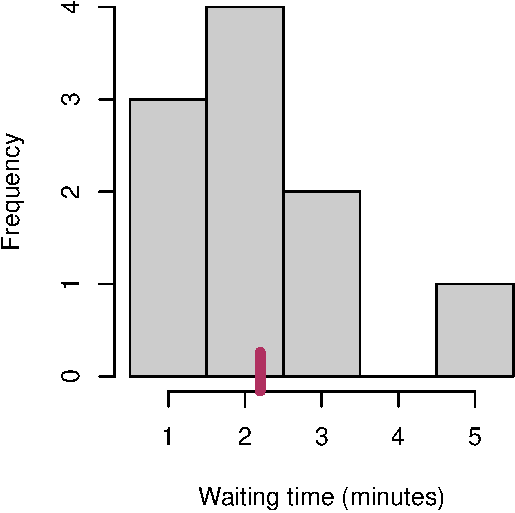
\includegraphics{QMS-EN_files/figure-latex/waittime-hist-1.pdf}
\caption{\label{fig:waittime-hist}Histogram of N=10 waiting times, with the mean marked.}
\end{figure}

\hypertarget{sec:median}{%
\subsection{median}\label{sec:median}}

The median (symbol \(Md\) or \(\tilde{x}\)) is the observation in the middle
of the order of observations \footnote{In American English, the strip of ground in the middle of a road is called the
  ``median (strip)'' (British English: ``central reservation''); this strip splits the road into
  two equally large halves.}. When we sort the scores of \(X\)
from smallest to largest, the median is the midpoint of the sorted
sequence. Half of the observations are smaller than the median,
and the other half is larger than the median.

For an odd number of observations, the middlemost observation is the median.
For an even number of observations, the median is usually formed from
the mean of the two middlemost observations.

\begin{center}\rule{0.5\linewidth}{0.5pt}\end{center}

\begin{quote}
\emph{Example 9.2}: The waiting times from Example 9.1
are ordered as follows:\\
1, 1, 1, 2, \emph{2, 2}, 2, 3, 3, 5.\\
The median is the mean of the two middlemost (italicised)
observations, so 2 minutes.
\end{quote}

\begin{center}\rule{0.5\linewidth}{0.5pt}\end{center}

The median is less sensitive than the mean to extreme values
of \(x\). In the above example, the extreme waiting time of 5 minutes
has a considerable influence on the mean. If we remove
that value, then the mean changes from 2.2 to 1.9 but the median is still
2. Extreme values thus have less great an influence on the
median then on the mean. Only if
the ordering of the observations changes, may the median also
change.

The median can be used with variables of ordinal, interval or ratio
level of measurement.

\hypertarget{mode}{%
\subsection{mode}\label{mode}}

The mode (adj. `modal') is the value or score of \(X\) which occurs
the most frequently.

\begin{center}\rule{0.5\linewidth}{0.5pt}\end{center}

\begin{quote}
\emph{Example 9.3}: In the waiting times from Example 9.1
the score 2 occurs the most often (\(4\times\)); this is the mode.
\end{quote}

\begin{center}\rule{0.5\linewidth}{0.5pt}\end{center}

\begin{quote}
\emph{Example 9.4}: In 2018, the mean income per household in the Netherlands was €29,500.
The modal income (per household) was between €18,000 and €20,000\footnote{\url{https://www.cbs.nl/nl-nl/visualisaties/inkomensverdeling}}. As such, in
2018, most households in the Netherlands fell within this income class.
\end{quote}

\begin{center}\rule{0.5\linewidth}{0.5pt}\end{center}

The mode is even less sensitive than the mean to extreme values of
\(x\). In the Example 9.2 above, it does not matter what the value of
the longest waiting time is: even if that observation has the value \(10\) or
\(1,000\), the mode remains invariably \(2\) (check it for yourself).

The mode can be used with variables of all levels of measurement.

\hypertarget{sec:harmonicmean}{%
\subsection{Harmonic mean}\label{sec:harmonicmean}}

If the dependent variable is a fraction or ratio,
like the speed with which a task is conducted, then
the (arithmetic) mean of formula \eqref{eq:average} does
not actually provide a good indication for the
most characteristic or central value. In that case, it is better
for you to use the harmonic mean:

\begin{equation}
  H = \frac{1}{\frac{1}{n} \sum\limits_{i}^n \frac{1}{x_i} } = \frac{n}{\sum\limits_{i}^n \frac{1}{x_i}}
  \label{eq:harmonicmean}
\end{equation}

\begin{center}\rule{0.5\linewidth}{0.5pt}\end{center}

\begin{quote}
\emph{Example 9.5}:
A student writes \(n=3\) texts. For the first text (500 words) (s)he takes
2.5 hours, for the second text (1,000 words) (s)he takes 4 hours, and
for the third text (300 words) (s)he takes 0.6 hours. What is this student's
mean speed of writing? The speeds of writing are respectively 200, 250 and 500
words per hour, and the ``normal'' (arithmetic) mean of these is
317 words per hour. Nevertheless, the ``actual'' mean is
\((500+1000+300)/(2.5+4+0.6)\) \(=1800/7.1=254\) words per hour. The high
writing speed of the short text counts for \(1/n\) parts in the arithmetic
mean, even though the text only contains \(300/1,800=1/6\)
of the total number of words.
\end{quote}

\begin{quote}
Since the dependent variable is a fraction (speed, words/hour),
the harmonic mean is a better central tendency. We firstly convert
the speed (words per time unit) into its inverse
(see \eqref{eq:harmonicmean}, in denominator, within sum sign),
i.e.~to \emph{time} per word: 0.005, 0.004, and 0.002 (time units per
word, see footnote\footnote{This is comparable with sports like rowing, swimming, cycling, ice skating, etc., where
  the time over an agreed distance is measured and compared, rather than the speed over an
  agreed time.}). We then average these times, to
a mean of 0.00366 hours per word, and finally we again take the
inverse of this. The harmonic mean speed of writing is then \(1/0.00366=273\)
words per hour, closer to the ``actual'' mean of 254 words per hour.
\end{quote}

\begin{center}\rule{0.5\linewidth}{0.5pt}\end{center}

\hypertarget{winsorized-mean}{%
\subsection{winsorized mean}\label{winsorized-mean}}

The great sensitivity of the normal (arithmetic) mean for
outliers can be restricted by changing the most extreme observations
into less extreme, more central observations. The
mean of these (partially changed) observations is called the
\emph{winsorized} mean.

\begin{center}\rule{0.5\linewidth}{0.5pt}\end{center}

\begin{quote}
\emph{Example 9.6}: The waiting times from Example 9.1
are ordered as follows:\\
1, 1, 1, 2, 2, 2, 2, 3, 3, 5.\\
For the 10\% winsorized mean, the 10\% of smallest observations (by
order) are made to equal the first subsequent larger value, and
the 10\% of largest observations are made to equal the last
preceding smaller value (changed values are italicised here):\\
\emph{1}, 1, 1, 2, 2, 2, 2, 3, 3, \emph{3}.\\
The winsorized mean over these changed values is
\(\overline{x}_w=2\) minutes.
\end{quote}

\begin{center}\rule{0.5\linewidth}{0.5pt}\end{center}

\hypertarget{trimmed-mean}{%
\subsection{trimmed mean}\label{trimmed-mean}}

An even more drastic intervention is to remove the most extreme observations
entirely. The mean of the remaining observations is called
the \emph{trimmed} mean. For a 10\% trim, we remove the lowermost 10\% \emph{and} the
uppermost 10\% of the observations;
as such, what remains is then only \((1- (2 \times (10/100))\times n\)
observations \citep{Wilcox12}.

\begin{center}\rule{0.5\linewidth}{0.5pt}\end{center}

\begin{quote}
\emph{Example 9.7}: The waiting times from Example 9.1
are again ordered as follows:\\
1, 1, 1, 2, 2, 2, 2, 3, 3, 5.\\
For the 10\% trimmed mean, the 10\% of smallest observations (by order) are removed,\\
and likewise the 10\% of largest observations
are removed:\\
1, 1, 2, 2, 2, 2, 3, 3.\\
The trimmed mean over these \(10-(.2)(10)=8\) remaining values here
is \(\overline{x}_t=2\) minutes.
\end{quote}

\begin{center}\rule{0.5\linewidth}{0.5pt}\end{center}

\hypertarget{comparison-of-central-tendencies}{%
\subsection{comparison of central tendencies}\label{comparison-of-central-tendencies}}

Figure \ref{fig:centraltendencies} illustrates the differences between
the various central tendencies, for asymmetrically distributed observations.

\begin{figure}
\centering
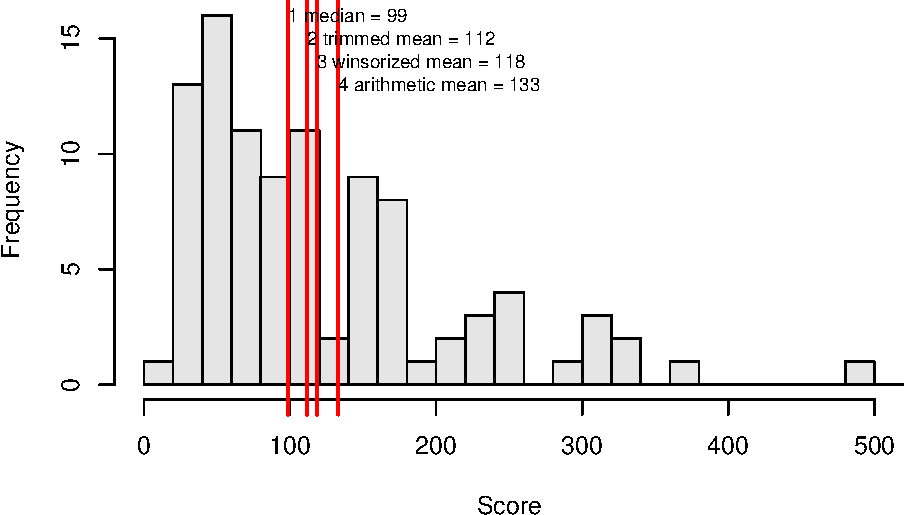
\includegraphics{QMS-EN_files/figure-latex/centraltendencies-1.pdf}
\caption{\label{fig:centraltendencies}Histogram of a variable with positively skewed (asymmetric) frequency distribution, with (1) the median, (2) the 10\% trimmed mean, (3) the 10\% winsorized mean, and (4) the arithmetic mean, indicated. The observed scores are marked along the horizontal axis.}
\end{figure}

The arithmetic mean is the most sensitive to extreme values:
the extreme values ``pull'' very hard at the mean. This influence
of extreme values is tempered in the winsorized mean, and
tempered even more in the trimmed mean. The higher the
trim factor (the percentage of the observations that have been changed or
removed), the more the winsorized and trimmed means will look like the median.
Indeed, with a trim factor of 50\%, out of all
the observations, only one (unchanged) observation remains, and that
is the median (check it for yourself). In
§\ref{sec:robustefficient} we will look further into the choice
for the appropriate measure for the centre of a distribution.

\hypertarget{sec:quartiles-and-boxplots}{%
\section{Quartiles and boxplots}\label{sec:quartiles-and-boxplots}}

The distribution of a variable is not only characterised by the
centre of the distribution but also by the degree of dispersion around
the centre, i.e.~how large the difference is between observations and the mean.
For instance, we not only want to know
what the mean income is but also how large the \emph{differences} in
income are.

\hypertarget{quartiles}{%
\subsection{Quartiles}\label{quartiles}}

Quartiles are a simple and useful measure for this \citep{Tukey77}.
We split the ordered observations into two halves; the dividing line
between these is the median. We then halve each of these halves again into quarters.
The quartiles are formed by the dividing lines between these
quarters; as such, there are three quartiles. The first quartile \(Q_1\) is the lowermost half's median,
\(Q_2\) is the median of all \(n\) observations, and the third quartile \(Q_3\) is the uppermost half's median.
Half of the observations (namely the second and third quarters) are
between \(Q_1\) and \(Q_3\). The distance between \(Q_1\) and \(Q_3\) is
called the ``interquartile range'' (IQR). This IQR is a first measure which
can be used for the dispersion of observations with respect to their
central value.

To illustrate, we use the fictive reading test scores shown in Table
\ref{tab:cito}.

\begin{longtable}[]{@{}cccc@{}}
\caption{\label{tab:cito} The scores of N=10 pupils on three sections of the CITO test,
taken in the final year of primary school in the Netherlands.}\tabularnewline
\toprule
Pupil & Reading & Arithmetic & Geography\tabularnewline
\midrule
\endfirsthead
\toprule
Pupil & Reading & Arithmetic & Geography\tabularnewline
\midrule
\endhead
1 & 18 & 22 & 55\tabularnewline
2 & 32 & 36 & 55\tabularnewline
3 & 45 & 34 & 38\tabularnewline
4 & 25 & 25 & 40\tabularnewline
5 & 27 & 29 & 48\tabularnewline
6 & 23 & 20 & 44\tabularnewline
7 & 29 & 27 & 49\tabularnewline
8 & 26 & 25 & 42\tabularnewline
9 & 20 & 25 & 57\tabularnewline
10 & 25 & 27 & 47\tabularnewline
\(\sum x\) & 270 & 270 & 475\tabularnewline
\(\overline{x}\) & 27.0 & 27.0 & 47.5\tabularnewline
\bottomrule
\end{longtable}

\begin{center}\rule{0.5\linewidth}{0.5pt}\end{center}

\begin{quote}
Example 9.8:
The scores for the reading section in
Table \ref{tab:cito} are
ordered as follows:\\
18, 20, 23, 25, 25, 26, 27, 29, 32, 45.\\
The median is \(Q_2=25.5\) (between the 5th and 6th observation in this
ranked list). The median of the lowermost half is \(Q_1=23\) and that of the
uppermost half is \(Q_3=29\). The interquartile range is
\(\textrm{IQR}=29-23=6\).
\end{quote}

\begin{center}\rule{0.5\linewidth}{0.5pt}\end{center}

\hypertarget{sec:outliers}{%
\subsection{Outliers}\label{sec:outliers}}

In the reading scores in Table \ref{tab:cito}, we encounter one extreme value, namely the score
45, which differs markedly from the mean. A marked value like this is referred to as an
``outlier''. The limit for what we consider to be an outlier
generally lies at \(1.5 \times \textrm{IQR}\). If a value is more than
\(1.5 \times \textrm{IQR}\) above or under \(Q_1\), we consider that
observation to be an outlier. Check these observations again (recall the principle of
diligence, see §\ref{sec:integrity-introduction}).

\begin{center}\rule{0.5\linewidth}{0.5pt}\end{center}

\begin{quote}
Example 9.9:
For the aforementioned reading scores in
Table \ref{tab:cito}, we found
\(Q_1=23\), \(Q_3=29\), and \(\textrm{IQR}=Q_3-Q_1=29-23=6\). The uppermost
limit value for outliers is
\(Q_3 + 1.5 \times \textrm{IQR} = 29 + 1.5 \times 6 = 29+9 = 38\). The
observation with the score 45 is above this limit value, and is therefore
considered to be an outlier.
\end{quote}

\begin{center}\rule{0.5\linewidth}{0.5pt}\end{center}

\hypertarget{sec:boxplot}{%
\subsection{Boxplots}\label{sec:boxplot}}

We can now show the frequency distribution of a variable with five
characteristics, the so-called ``five-number summary'', namely the minimum value, \(Q_1\),
median, \(Q_3\), and maximum value. These five characteristics are represented graphically
in a so-called ``boxplot'', see
Figure \ref{fig:cito-boxplot}
for an example \citep[ §2C]{Tukey77}.

\begin{figure}
\centering
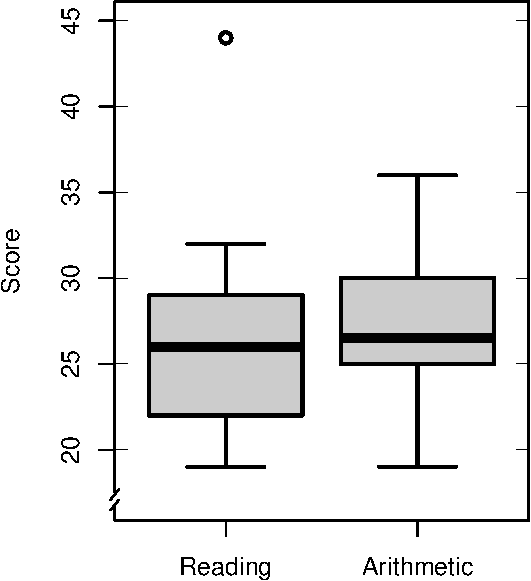
\includegraphics{QMS-EN_files/figure-latex/cito-boxplot-1.pdf}
\caption{\label{fig:cito-boxplot}Boxplots of the scores of \(N=10\) pupils on the Reading and Arithmetic sections of the CITO test (see Table 9.1), with outliers marked as open circles. The observed scores are marked along the vertical axes.}
\end{figure}

The box spans (approximately) the area from \(Q_1\) to \(Q_3\), and
thus spans the central half of the observations. The thicker line in the
box marks the median. The lines extend to the smallest and largest
values \emph{which are not outliers} \footnote{In a classic boxplot, the lines extend to the minimum and maximum \citep{Tukey77} and
  outliers are not indicated separately.}. The separate outliers
are indicated here with a distinct symbol.

\hypertarget{sec:measures-of-dispersion}{%
\section{Measures of dispersion}\label{sec:measures-of-dispersion}}

\hypertarget{sec:variance}{%
\subsection{Variance}\label{sec:variance}}

Another way to show the dispersion of observations would be to look at how
each observation deviates from the mean, thus \((x_i-\overline{x})\). However, if we
add up all the deviations, they always total zero! After all, the positive and negative
deviations cancel each other out (check that out for yourself in
Table \ref{tab:cito}).
Instead of calculating the mean of the deviations themselves, we thus calculate the mean
of the squares of those deviations. Both the positive and negative deviations
result in positive squared deviations. We then calculate the mean of all
those squared deviations, i.e.~we add them up and divide them by
\((n-1)\), see Footnote\footnote{We divide by \(n-1\) and not by \(n\), to get a better estimation of the dispersion in the
  \emph{population}. In this way, we take into account the fact that we are using a characteristic of the
  sample (namely the mean) to determine the dispersion. If you are only interested in the
  dispersion in your \emph{sample} of observations, and not in the population, divide it by \(n\).}. We call the result the
\emph{variance}, indicated by the symbol \(s^2\):
\begin{equation}
  s^2 = \frac{ \sum (x_i - \overline{x})^2 } {n-1}
  \label{eq:variance}
\end{equation}

The numerator of
this fraction is referred to as the ``sum of squared deviations'' or
``sum of squares'' (SS) and the denominator is referred to as the number of
``degrees of freedom'' of the numerator (d.f.; see
§\ref{sec:ttest-freedomdegrees}).

Nowadays, we always calculate the variance with a calculator
or computer.

\hypertarget{sec:standarddeviation}{%
\subsection{standard deviation}\label{sec:standarddeviation}}

To calculate the above variance, we squared the deviations of the
observations. As such, the variance is a quantity which is not expressed
in the original units (e.g.~seconds, cm, score),
but in squared units (e.g.~\(\textrm{s}^2\),
\(\textrm{cm}^2\), \(\textrm{score}^2\)). In order to return to the
original units, we take the square root of the variance. We call the result the
\emph{standard deviation}, indicated by the symbol \(s\):

\begin{equation}
  s = \sqrt{s^2} = \sqrt{ \frac{ \sum (x_i - \overline{x})^2 } {n-1} }
  \label{eq:standarddeviation}
\end{equation}

\begin{center}\rule{0.5\linewidth}{0.5pt}\end{center}

\begin{quote}
Example 9.10:
The mean of the previously stated reading scores in
Table \ref{tab:cito} is
\(27.0\), and the deviations are as follows:\\
-9, 5, 18, -2, 0, -4, 2, -1, -7, -2.\\
The squared deviations are 81, 25, 324, 4, 0, 16, 4, 1, 49, 4.\\
The sum of these squared deviations is 508, and the variance is
\(s^2=508/9=56.44\). The standard deviation is the root of the
variance, thus \(s=\sqrt{508/9}=7.5\).
\end{quote}

\begin{center}\rule{0.5\linewidth}{0.5pt}\end{center}

The variance and standard deviation can only be used with variables
of the interval or ratio level of measurement. The variance and
standard deviation can also be based again on the winsorized or trimmed
collection of observations.

We need the standard deviation
(a) when we want to convert the raw
observations to standard scores (see §\ref{sec:standardscores} below),
(b) when we want to describe a variable
which is normally distributed (see §\ref{sec:normaldistribution}, and
(c) when we want to test hypotheses with the help of a normally distributed variable (see
§\ref{sec:ttest-onesample} et seq.).

\hypertarget{mad}{%
\subsection{MAD}\label{mad}}

Besides standard deviation, there is also a robust counterpart
which does not use the mean. This measure is therefore less
sensitive for outliers (robuster), which is sometimes useful.

For this, we look for the deviation of every observation from
the median (not the mean). We then take the absolute value
of these deviations\footnote{Positive deviations remain unchanged, negative deviations are reversed.} (not the square). Finally, we
determine again the median of these absolute deviations (not the mean).
We call the result the ``median absolute deviation'' (MAD):
\begin{equation}
  \textrm{MAD} = k ~~ Md ( |x_i - Md(x) |)
  \label{eq:MAD}
\end{equation}

We normally use \(k=1.4826\) as a constant here; with this scale factor the MAD
usually roughly matches the standard deviation \(s\), if \(x\) is
normally distributed (§\ref{sec:normaldistribution}).

\begin{center}\rule{0.5\linewidth}{0.5pt}\end{center}

\begin{quote}
Example 9.11:
The median of the previously mentioned reading scores in
Table \ref{tab:cito} is
25.5, and the deviations from the median are as follows:\\
-7.5, 6.5, 19.5, -0.5, 1.5, -2.5, 3.5, 0.5, -5.5, -0.5.\\
The ordered absolute deviations are\\
0.5, 0.5, 0.5, 1.5, \emph{2.5, 3.5}, 5.5, 6.5, 7.5, 19.5.\\
The median of these 10 absolute deviations is 3, and
\(\textrm{MAD} = 1.4826 \times 3 = 4.4478\). Notice that the MAD
is smaller than the standard deviation, amongst others because the MAD is less sensitive
for the extreme value \(x_3=45\).
\end{quote}

\begin{center}\rule{0.5\linewidth}{0.5pt}\end{center}

\hypertarget{sec:significantfigures}{%
\section{On significant figures}\label{sec:significantfigures}}

\hypertarget{sec:significantfigures-means}{%
\subsection{Mean and standard deviation}\label{sec:significantfigures-means}}

A mean result is shown in a limited number of significant figures, i.e.~
a limited number of figures, counted from left to right, ignoring the decimal place.
The mean result's number of significant figures must be equal to the
number of significant figures of the \emph{number of observations} from which the
mean is calculated. (Other figures in the mean result are not precisely
determined.) The mean result must firstly be rounded to the
appropriate number of significant figures, before the result is interpreted
further, see
Table \ref{tab:signiffiguresmean}.

\begin{longtable}[]{@{}clcc@{}}
\caption{\label{tab:signiffiguresmean} The number of significant figures in the reported mean is
equal to the number of significant figures of the number of observations.}\tabularnewline
\toprule
Num.obs. & Num.signif.figures & example mean & reported as\tabularnewline
\midrule
\endfirsthead
\toprule
Num.obs. & Num.signif.figures & example mean & reported as\tabularnewline
\midrule
\endhead
\(1\dots9\) & 1 & 21/8 = 2.625 & 3\tabularnewline
\(10\dots99\) & 2 & 57/21 = 2.714286 & 2.7\tabularnewline
\(100\dots999\) & 3 & 317/120 = 2.641667 & 2.64\tabularnewline
\(1000\dots9999\) & 4 & 3179/1234 = 2.576175 & 2.576\tabularnewline
\bottomrule
\end{longtable}

The number of significant figures in the reported standard deviation is
the same as in the mean, in accordance with
Table \ref{tab:signiffiguresmean}.

\hypertarget{background}{%
\subsubsection{Background}\label{background}}

Let us assume that I have measured the distance from my house to my work
along a fixed route a number of times. The mean of those measurements
supposedly amounts to \(2.954321\) km. By reporting the mean with 7 figures,
I am suggesting here that I know precisely that the distance is \(2954321\) millimetres,
and at most \(1\) mm more or less:
the last figure is estimated or rounded off. The number of significant figures
(in this example 7) indicates the degree of precision. In this example, the
suggested precision of 1 mm is clearly
wrong, amongst other reasons because the start point and end point cannot be determined
within a millimetre. It is thus usual to report the mean of the measured
distance with a number of significant figures which indicates the precision
of those measurements and of the mean, e.g.~
\(3.0\)~km (by car or bike) of \(2.95\)~km (by foot).

The same line of thought is applicable when measuring a characteristic
by means of a survey question. With \(n=15\) respondents, the average score
might be \(43/15 \approx 2.86667\). However, the precision
in this example is not as good as this decimal number suggests. In fact,
here one deviant answer already brings about a deviation of
\(\pm0.06667\) in the mean. Besides, a mean score
is always the result of a division operation, and
``{[}for{]} quantities created from measured quantities by multiplication and division, the calculated result should have as many significant figures as the measured number with the least number of significant figures'' \footnote{\url{https://en.wikipedia.org/wiki/Significant_figures}}.
In this example, the mean's numerator (\(43\)) and its denominator (\(15\)) both consist
of 2 significant figures. The mean score should be reported as \(2.9\) points, with only
one figure after the decimal point.

\hypertarget{percentages}{%
\subsection{Percentages}\label{percentages}}

A percentage is a fraction, multiplied by \(100\).
Use and report a rounded off percentage (i.e.~two significant
figures) only if the fraction's numerator is larger
than 100 (observations, instances). If the numerator is smaller than 100
(observations, instances), then percentages are misleading,
see Table \ref{tab:signiffigurepercentage}.

\begin{longtable}[]{@{}rccc@{}}
\caption{\label{tab:signiffigurepercentage} The number of significant figures in the reported
proportion (or percentage) is related to the number of significant figures of the number
of observations in the denominator of the fraction.}\tabularnewline
\toprule
num.obs.(denominator) & num.signif.figures & example fraction & report as\tabularnewline
\midrule
\endfirsthead
\toprule
num.obs.(denominator) & num.signif.figures & example fraction & report as\tabularnewline
\midrule
\endhead
\(1\dots9\) & 1 & 3/8 = 0.4 & 3/8\tabularnewline
\(10\dots99\) & 2 & 21/57 = 0.36 & 21/57\tabularnewline
\(100\dots999\) & 3 & 120/317 = 0.378 & 38\%\tabularnewline
\(1000\dots9999\) & 4 12 & 34/3179 = 0.3882 & 38.8\%\tabularnewline
\bottomrule
\end{longtable}

\hypertarget{background-1}{%
\subsubsection{Background}\label{background-1}}

The rules for percentages arise from those in
§\ref{sec:significantfigures-means} applied to division operations.
If the denominator is larger than 100, the percentage (with two significant
figures) is the result of a scaling ``down'' (from a denominator
larger than 100 to a denominator of precisely 100 percentage points).
The percentage scale is less precise than the original
ratio; the percentages are rounded off to two significant figures;
the percentage's last significant figure is thus secured.

However, if the denominator is smaller than 100, then the percentage (with
two significant figures) is the result of a ``scaling upwards'' (from a denominator
smaller than 100 to a denominator of exactly 100 percentage points). The percentage
scale then suggests a
pseudo-precision which was not present in the original fraction,
and the precision of the percentage scale is false. As such, if the denominator is
smaller than 100, percentages are misleading.

\begin{center}\rule{0.5\linewidth}{0.5pt}\end{center}

\begin{quote}
Example 9.12:
In a course of 29 students, 23 students passed. In this case, we often
speak of a course return of \(23/29=\) 79\%. However, a rendering as a
percentage is misleading in this case. To see this, let us look
at the 6 students who failed. You can reason that the number of 6 failed
students has a rounding error of \(1/2\) student(s); when converted to the
percentage scale this rounding error is also thereby increased so that
the percentages are less precise than the whole percentages (2
significant figures) suggest. Or put otherwise: the number of 6
failed students (i.e.~a number with one significant figure) means we have
to render the proportion with only one significant figure, and thus not
as a percentage. It is preferable to report the proportion itself (\(23/29\)), or
the ``odds'' (\(23/6=4\)) rounded off to the correct number of significant
figures\footnote{These ``odds'' indicate that there are 23 successful students to 6 failed students, i.e., rounded up, 4 successful students for every failed student.}.
\end{quote}

\begin{center}\rule{0.5\linewidth}{0.5pt}\end{center}

On the basis of the same considerations, a percentage with one decimal
place (i.e.~with three significant figures, e.g.~``36.1\%'') is only
meaningful if the ratio or fraction's denominator is larger than 1000.

\begin{center}\rule{0.5\linewidth}{0.5pt}\end{center}

\begin{quote}
Example 9.13:
In 2013, 154 students began a two-year research master's degree. After
2 years, 69 of them had graduated. The nominal return for this cohort is
thus \(69/154=\) 0.448052, which should be rounded off and reported as 44\%
(not as 44.81\%).
\end{quote}

\begin{center}\rule{0.5\linewidth}{0.5pt}\end{center}

\hypertarget{sec:robustefficient}{%
\section{Making choices}\label{sec:robustefficient}}

You can describe the distribution of a variable in various
manners.
If variable \(X\) is measured on the interval or ratio level of measurement,
always begin with a histogram (§\ref{sec:histograms})
and a boxplot (§\ref{sec:boxplot}).

The centre measures and dispersion measures can be arranged
as in Table \ref{tab:centredispersionmeasures}.

\begin{longtable}[]{@{}lcc@{}}
\caption{\label{tab:centredispersionmeasures} Overview of discussed centre measures and dispersion measures. For assumptions abbreviated to \emph{(a \& b \& c)}, see text below table.}\tabularnewline
\toprule
Distribution & Centre measure & Dispersion measure\tabularnewline
\midrule
\endfirsthead
\toprule
Distribution & Centre measure & Dispersion measure\tabularnewline
\midrule
\endhead
all & median & quartiles, IQR, MAD\tabularnewline
\ldots{} & trimmed or wins. mean & trimmed or wins.std.dev.\tabularnewline
(a \& b \& c) & mean & standard deviation\tabularnewline
\bottomrule
\end{longtable}

The most \textbf{robust} measures are
at the top (median, quartiles, IQR, MAD). These measures are robust:
they are less sensitive for outliers or for potential \emph{a}symmetry in the
frequency distribution, as the examples in this chapter show.

The most \textbf{efficient} measures are at the bottom of
Table \ref{tab:centredispersionmeasures}: mean and standard deviation.
These measures are efficient: they represent the centre and the dispersion
the best, they have themselves the smallest standard deviation, and they need
the (relatively) smallest number of observations for this. The other measures
occupy a between position: the trimmed measures are somewhat more robust,
and the winsorized measures somewhat more efficient.

However, the most efficient measures also demand the furthest reaching
assumptions (and the most robust measures demand the fewest assumptions).
These efficient measures are only meaningful if the distribution of \(X\)
satisfies three assumptions: (a) the distribution is more or less
symmetrical, i.e.~the left and right halves of the histogram and
the uppermost and lowermost halves of the boxplot look like each other's
mirror image, (b) the distribution is unimodal, i.e.~the distribution has
a unique mode, and (c) the distribution contains no or hardly any outliers.
Inspect these assumptions in the histogram and the boxplot of \(X\). If one
of these assumptions is not satisfied, then it is better to use
more robust measures to describe the distribution.

\hypertarget{sec:standardscores}{%
\section{Standard scores}\label{sec:standardscores}}

It can sometimes be useful to compare scores which are measured on
different scales. Example: Jan got an 8 as his final grade for\\
maths at Dutch secondary school, and his IQ is 136. Is the deviation of Jan with
respect to the mean as large on both of the scales? To answer a question
like this, we have to express the scores of the two variables on the
same measurement scale. We do so by converting the raw scores to
standard scores, or z-scores. For this, we take the deviation of every
score with respect to the mean, and we divide the deviation by the
standard deviation:

\begin{equation}
    z_i = \frac{(x_i-\overline{x})}{s_x}
   \label{eq:zscores}
\end{equation}

The standard score or z-score
thus represents the distance of the \(i\)'the observation to the mean
of \(x\), expressed in units of standard deviation. For a
standard score of \(z=-1\), the observed score is precisely \(1 \times s\)
below the average \(\overline{x}\). For a standard score of \(z=+2\),
then the observed score is precisely \(2 \times s\) above the
mean\footnote{Check: \(z = +2 = \frac{(x_i-\overline{x})}{s_x}\), thus \(2 s = (x_i-\overline{x})\), thus \(x_i = \overline{x}+2s\).}.

Z-scores are also useful for comparing two variables which
are in fact measured on the same scale (for example, a scale of
\(1 \dots 100\)), but which nevertheless have different means and/or
standard deviations, like the scores in
Tabel \ref{tab:cito}.
In Chapter \ref{ch:probability-distributions}, we will work more with z-scores.

The standard score or z-score has two useful characteristics which you
should remember. Firstly, the mean is always equal to zero:
\(\overline{z}=0\), and, secondly, the standard deviation is equal to 1:
\(s_z = 1\). (These characteristics follow from the definition in
formula \eqref{eq:zscores}; we omit the mathematical proof here.) Thus,
transformation from a collection of observations to
standard scores or z-scores always yields a distribution with
a mean of zero and a standard deviation of one. Do remember that
this transformation to standard scores is only meaningful, provided that and
to the extent that the mean and the standard deviation are also meaningful measures
to describe the distribution of \(x\) (see §\ref{sec:robustefficient}).

\hypertarget{spss-3}{%
\section{SPSS}\label{spss-3}}

For \textbf{histogram, percentiles and boxplot}:

\begin{verbatim}
Analyze > Descriptive Statistics > Explore...
\end{verbatim}

Select variable (drag to Variable(s) panel)\\
Choose \texttt{Plots}, tick: \texttt{Histogram}, and confirm with \texttt{Continue}\\
Choose \texttt{Options}, tick: \texttt{Percentiles}, and confirm with \texttt{Continue} and
afterwards with \texttt{OK}.\\
The output comprises descriptive statistics and histogram and
boxplot.

For \textbf{descriptive characteristic values}:~

\begin{verbatim}
Analyze > Descriptive Statistics > Descriptives...
\end{verbatim}

Select variable (drag to Variable(s) panel)\\
Choose \texttt{Options}; tick:
\texttt{Mean,\ Sum,\ Std.deviation,\ Variance,\ Minimum,\ Maximum}, and confirm with
\texttt{Continue} and afterwards with \texttt{OK}.\\
The output comprises the requested statistical characteristics of the variable's distribution.\\

For \textbf{median}:\\

\begin{verbatim}
Analyze > Compare Means > Means...
\end{verbatim}

Select variable (drag to Variable(s) panel)\\
Choose \texttt{Options}; tick:
\texttt{Mean,\ Number\ of\ cases,\ Standard\ deviation,\ Variance,\ Minimum,\ Maximum}
and also \texttt{Median}, and confirm with \texttt{Continue} and afterwards with \texttt{OK}.\\
The output comprises the requested statistical characteristics of the variable's distribution.\\

Calculate and save \textbf{Standard scores} in a new column:\\

\begin{verbatim}
Analyze > Descriptive Statistics > Descriptives...
\end{verbatim}

Select variables (drag to Variable(s) panel)\\
Tick: \texttt{Save\ standardized\ values\ as\ variables} and confirm with \texttt{OK}.\\
The new variable(s) with z-scores are added as new
column(s) to the data file.\\

\hypertarget{r-3}{%
\section{R}\label{r-3}}

For \textbf{quartiles and boxplot} like Figure \ref{fig:cito-boxplot}, we use the commands \texttt{fivenum}, \texttt{quantile}, and \texttt{boxplot}:

\begin{Shaded}
\begin{Highlighting}[]
\KeywordTok{require}\NormalTok{(foreign) }\CommentTok{\# for foreign::read.spss}
\NormalTok{cito \textless{}{-}}\StringTok{ }\KeywordTok{read.spss}\NormalTok{(}\StringTok{"data/cito.sav"}\NormalTok{)}
\CommentTok{\# Columns in \textasciigrave{}cito.sav\textasciigrave{} have Dutch names:}
\CommentTok{\# in Dutch: Leerling Lezen Rekenen Wereldorientatie stadplat rek.f}
\CommentTok{\# in English: Pupil Reading Arithmetic Geography UrbRural Arith.factor}
\KeywordTok{fivenum}\NormalTok{(cito}\OperatorTok{$}\NormalTok{Lezen) }\CommentTok{\# minimum, Q1, median, Q3, maximum}
\end{Highlighting}
\end{Shaded}

\begin{verbatim}
## [1] 19 22 26 29 44
\end{verbatim}

\begin{Shaded}
\begin{Highlighting}[]
\KeywordTok{quantile}\NormalTok{(cito}\OperatorTok{$}\NormalTok{Lezen, }\KeywordTok{c}\NormalTok{( }\DecValTok{1}\OperatorTok{/}\DecValTok{4}\NormalTok{, }\DecValTok{3}\OperatorTok{/}\DecValTok{4}\NormalTok{ ) ) }\CommentTok{\# Q1 and Q3, calculated differently }
\end{Highlighting}
\end{Shaded}

\begin{verbatim}
##   25%   75% 
## 22.75 28.75
\end{verbatim}

\begin{Shaded}
\begin{Highlighting}[]
\NormalTok{op \textless{}{-}}\StringTok{ }\KeywordTok{par}\NormalTok{(}\DataTypeTok{mar=}\KeywordTok{c}\NormalTok{(}\DecValTok{4}\NormalTok{,}\DecValTok{4}\NormalTok{,}\DecValTok{1}\NormalTok{,}\DecValTok{2}\NormalTok{)}\OperatorTok{+}\FloatTok{0.1}\NormalTok{) }\CommentTok{\# smaller margins}
\KeywordTok{with}\NormalTok{(cito, }
  \KeywordTok{boxplot}\NormalTok{(Lezen, Rekenen, }\DataTypeTok{col=}\StringTok{"grey80"}\NormalTok{, }\DataTypeTok{lwd=}\DecValTok{2}\NormalTok{, }\DataTypeTok{lty=}\DecValTok{1}\NormalTok{, }\DataTypeTok{ylab=}\StringTok{"Score"}\NormalTok{, }\DataTypeTok{ylim=}\KeywordTok{c}\NormalTok{(}\DecValTok{17}\NormalTok{,}\DecValTok{45}\NormalTok{) )}
\NormalTok{)}
\KeywordTok{axis}\NormalTok{(}\DataTypeTok{side=}\DecValTok{1}\NormalTok{, }\DataTypeTok{at=}\KeywordTok{c}\NormalTok{(}\DecValTok{1}\NormalTok{,}\DecValTok{2}\NormalTok{), }\DataTypeTok{labels=}\KeywordTok{c}\NormalTok{(}\StringTok{"Reading"}\NormalTok{,}\StringTok{"Arithmetic"}\NormalTok{) )}
\NormalTok{plotrix}\OperatorTok{::}\KeywordTok{axis.break}\NormalTok{(}\DataTypeTok{axis=}\DecValTok{2}\NormalTok{) }\CommentTok{\# break in left Y{-}aixs}
\KeywordTok{rug}\NormalTok{(cito}\OperatorTok{$}\NormalTok{Lezen, }\DataTypeTok{side=}\DecValTok{2}\NormalTok{) }\CommentTok{\# markings on left Y{-}axis}
\KeywordTok{rug}\NormalTok{(cito}\OperatorTok{$}\NormalTok{rekenen, }\DataTypeTok{side=}\DecValTok{4}\NormalTok{) }\CommentTok{\# markings on right Y{-}axis}
\end{Highlighting}
\end{Shaded}

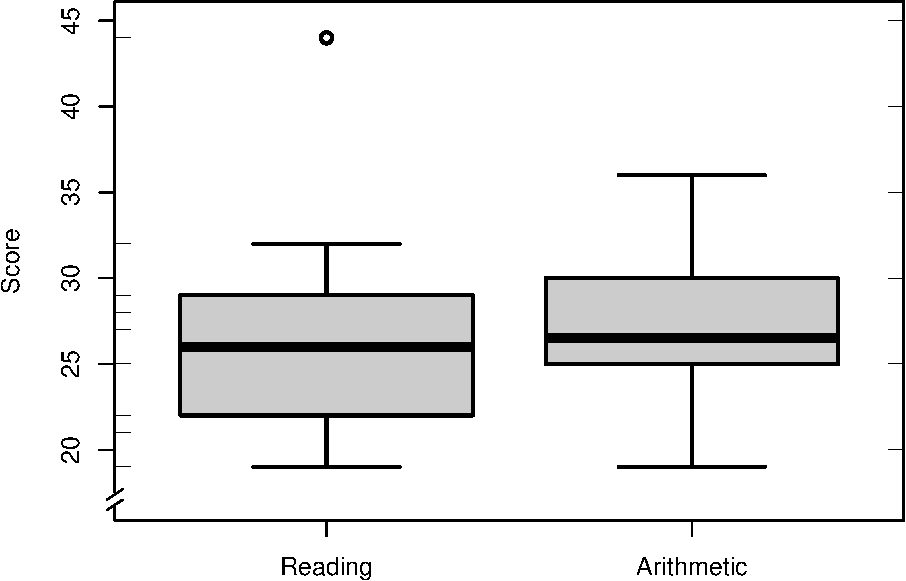
\includegraphics{QMS-EN_files/figure-latex/cito-summary-boxplot-1.pdf}

Many \textbf{central tendencies} are pre-programmed as functions in R:

\begin{Shaded}
\begin{Highlighting}[]
\KeywordTok{mean}\NormalTok{(cito}\OperatorTok{$}\NormalTok{Lezen) }\CommentTok{\# mean}
\end{Highlighting}
\end{Shaded}

\begin{verbatim}
## [1] 27.2
\end{verbatim}

\begin{Shaded}
\begin{Highlighting}[]
\NormalTok{psych}\OperatorTok{::}\KeywordTok{winsor.mean}\NormalTok{(cito}\OperatorTok{$}\NormalTok{Lezen, }\DataTypeTok{trim=}\NormalTok{.}\DecValTok{1}\NormalTok{) }\CommentTok{\# winsorized mean, from psych package}
\end{Highlighting}
\end{Shaded}

\begin{verbatim}
## [1] 26.3
\end{verbatim}

\begin{Shaded}
\begin{Highlighting}[]
\KeywordTok{mean}\NormalTok{(cito}\OperatorTok{$}\NormalTok{Lezen, }\DataTypeTok{trim=}\NormalTok{.}\DecValTok{1}\NormalTok{) }\CommentTok{\# trimmed mean}
\end{Highlighting}
\end{Shaded}

\begin{verbatim}
## [1] 26.125
\end{verbatim}

\begin{Shaded}
\begin{Highlighting}[]
\KeywordTok{median}\NormalTok{(cito}\OperatorTok{$}\NormalTok{Lezen)   }\CommentTok{\# median}
\end{Highlighting}
\end{Shaded}

\begin{verbatim}
## [1] 26
\end{verbatim}

Various \textbf{dispersion measures} are also pre-programmed:

\begin{Shaded}
\begin{Highlighting}[]
\KeywordTok{var}\NormalTok{(cito}\OperatorTok{$}\NormalTok{Lezen)  }\CommentTok{\# variance}
\end{Highlighting}
\end{Shaded}

\begin{verbatim}
## [1] 50.17778
\end{verbatim}

\begin{Shaded}
\begin{Highlighting}[]
\KeywordTok{sd}\NormalTok{(cito}\OperatorTok{$}\NormalTok{Lezen)   }\CommentTok{\# standard deviation, sd(x) = sqrt(var(x))}
\end{Highlighting}
\end{Shaded}

\begin{verbatim}
## [1] 7.083627
\end{verbatim}

\begin{Shaded}
\begin{Highlighting}[]
\KeywordTok{mad}\NormalTok{(cito}\OperatorTok{$}\NormalTok{Lezen)  }\CommentTok{\# MAD}
\end{Highlighting}
\end{Shaded}

\begin{verbatim}
## [1] 5.1891
\end{verbatim}

In contrast, we have to calculate \textbf{standard scores} ourselves, and save them ourselves as a
new variable, called here \texttt{zReading} (note the parentheses in the first command line):

\begin{Shaded}
\begin{Highlighting}[]
\CommentTok{\# standardized (or z) reading scores}
\NormalTok{zReading \textless{}{-}}\StringTok{ }\NormalTok{(cito}\OperatorTok{$}\NormalTok{Lezen}\OperatorTok{{-}}\KeywordTok{mean}\NormalTok{(cito}\OperatorTok{$}\NormalTok{Lezen)) }\OperatorTok{/}\StringTok{ }\KeywordTok{sd}\NormalTok{(cito}\OperatorTok{$}\NormalTok{Lezen) }
\KeywordTok{head}\NormalTok{(zReading) }\CommentTok{\# first few observations of variable zReading}
\end{Highlighting}
\end{Shaded}

\begin{verbatim}
## [1] -1.1575990  0.6776189  2.3716662 -0.3105753  0.1129365 -0.7340872
\end{verbatim}

\hypertarget{ch:probability-distributions}{%
\chapter{Probability distributions}\label{ch:probability-distributions}}

\hypertarget{sec:probabilities}{%
\section{Probabilities}\label{sec:probabilities}}

Calling behind the wheel increases the chance of an accident \citep{Bhar13}.
The average chance of precipitation in the Netherlands is 7\%. My order has a
10\% chance of being delivered a day later than promised. Chances and probabilities
play an important role in our daily lives, and also in academic research. After all,
many hypotheses are probabilistic in nature (see Chapter
\ref{ch:research}): hypotheses make statements about a
difference in the \emph{chances} of outcomes. To be able to draw conclusions with
respect to these probabilistic hypotheses, we need to know something about
probabilities and
probability distributions. This is the subject of the present chapter.

As an introduction, let us take a look at a Dutch \emph{Scrabble} game.
The game contains a bag with 102 tiles inside, each of which has a letter on it
\footnote{However, two of the tiles are blank (without any letter); later in this section we will remove these blank tiles from the bag.}. Of the 102 tiles, 6 have the letter A on them. If I take one tile from a
full and well-mixed bag, what is the chance that I draw the letter A? The
probability-of-the-outcome-A is referred to as \(P(\textrm{A})\), with the \(P\) of
\emph{Probabilitas} (Lat. ``chance, probability''), and can be determined as
\begin{equation}
    P(\textrm{A})=
    \frac{\textrm{number of A's}}{\textrm{total number of tiles}}= 
    \frac{6}{102} = 0.0588
  \label{eq:probability-scrabble-1-A}
\end{equation}

The probability of an event is expressed as a proportion, a number between
\(0\) and \(1\), or as a percentage, i.e.~a proportion in units of \(1/100\).
A probability can never be smaller than \(0\) and can never be larger than
1: after all, the probability is the proportion between the number
of specific outcomes (numerator) and the total number of possible outcomes
(denominator) (see
formula \eqref{eq:probability-scrabble-1-A}), where the numerator can never be larger
than the denominator \citep{SK01}.

When two outcomes mutually exclude each other, as is the case for
the outcomes A or B in our Scrabble example, then we may \emph{sum up}
these outcomes (rule of sum, or addition principle, or \emph{OR} rule).
The probability of outcome A \emph{or}
outcome B (where outcomes A and B exclude each other), is the \emph{sum}
of \(P(\textrm{A})\) and \(P(\textrm{B})\):
\begin{equation}
    P(\textrm{A or B}) = P(\textrm{A}) + P(\textrm{B})
  \label{eq:probability-sumrule}
\end{equation}

\begin{center}\rule{0.5\linewidth}{0.5pt}\end{center}

\begin{quote}
\emph{Example 10.1:}
In our Scrabble example, \(P(\textrm{A})=\frac{6}{102}\) and
\(P(\textrm{B})=\frac{2}{102}\). As such, the probability of outcome A-or-B is
\(P(\textrm{A or B})=P(\textrm{A})+P(\textrm{B})=6/102+2/102=8/102=.0784\).
\end{quote}

\begin{center}\rule{0.5\linewidth}{0.5pt}\end{center}

If I take one tile from a full and well-mixed bag, then two
complementary outcomes are possible: Either I draw an A, or I do \emph{not}
draw an A. The outcomes again mutually exclude each other so we may
sum up the probabilities too. Moreover, the
outcomes are complementary, i.e the outcome can only have one
of these two possible outcomes. The respective probabilities of these
complementary events are also complementary, i.e.~these
respective probabilities sum up to precisely \(1\) =100\% (complement rule).
After all, there is a 100\% probability that the outcome is one of
the two possible outcomes of the draw. If we already know \(P(\textrm{A})\),
we can easily calculate the probability of the complementary
outcome:
\begin{align}
    P(\textrm{A}) + P(\textrm{not-A}) & = & 1\\
    P(\textrm{A}) & = & 1 - P(\textrm{not-A})\\
    P(\textrm{not-A}) & = & 1 - P(\textrm{A})
    \label{eq:complementrule}
\end{align}

\begin{center}\rule{0.5\linewidth}{0.5pt}\end{center}

\begin{quote}
\emph{Example 10.2:}
In our Scrabble example, \(P(\textrm{A})=\frac{6}{102}\). As such, the probability
of the not-A outcome is
\(P(\textrm{not-A})= 1 - P(\textrm{A}) = 1 - \frac{6}{102} = \frac{96}{102} = .9412\).
\end{quote}

\begin{center}\rule{0.5\linewidth}{0.5pt}\end{center}

As a thought experiment, let us now take a second Scrabble game, and, from it, take
a second tile bag which is equally full and well-mixed.
Without looking, we will now take a letter tile from each bag. There are now two
events or outcomes, namely the outcome of the first draw (from the first
bag), and the outcome of the second draw (from the second bag).
These two outcomes do not mutually exclude each other, since they
have no mutual influence on each other. After all, the second
bag's outcome is not influenced by the first bag's outcome, and vice versa. As
such, we say that these outcomes are \emph{independent} of each other. When the outcomes
are indeed independent of each other, we calculate the probability of a
combination of the outcomes by \emph{multiplication} (multiplication
principle, or product rule, or \emph{AND} rule).\\
The probability of the combination of outcome A \emph{and} outcome B
(where outcomes A and B are independent of each other), is the
\emph{product} of \(P(\textrm{A})\) and \(P(\textrm{B})\):
\begin{equation}
    P(\textrm{A and B}) = P(\textrm{A}) \times P(\textrm{B})
  \label{eq:probability-productrule}
\end{equation}

\begin{center}\rule{0.5\linewidth}{0.5pt}\end{center}

\begin{quote}
\emph{Example 10.3:}
In our Scrabble example, \(P(\textrm{A})=\frac{6}{102}\) and
\(P(\textrm{B})=\frac{2}{102}\). The probability of outcome A with the first
bag \emph{and} B with the second bag is
\(P(\textrm{A and B})=P(\textrm{A}) \times P(\textrm{B})=\frac{6}{102} \times \frac{2}{102} = .0012\).
\end{quote}

\begin{center}\rule{0.5\linewidth}{0.5pt}\end{center}

\begin{quote}
\emph{Example 10.4:}
In our Scrabble game, \(P(\textrm{vowel})=\frac{38}{102}\). The probability
of drawing a vowel (A, E, I, O, U, Y) from the first bag \emph{and} a
vowel from the second bag is
\(P(\textrm{vowel-and-vowel})=P(\textrm{first vowel}) \times P(\textrm{second vowel})=\frac{38}{102} \times \frac{38}{102} = (\frac{38}{102})^2 = .1388\).
\end{quote}

\begin{center}\rule{0.5\linewidth}{0.5pt}\end{center}

\hypertarget{sec:binomial-distribution}{%
\section{Binomial probability distribution}\label{sec:binomial-distribution}}

For the remainder of this chapter, we will adopt two changes to the
Scrabble game. Firstly, we will remove the 2 blank, letter-less titles
from the bag. There are now precisely 100 tiles left, of which
38 have a vowel (\(V\)) and 62 have a consonant (\(C\)). Accordingly, there are only
two possible outcome categories left and these mutually exclude each other.
We call such a variable of the nominal level of measurement,
with precisely two categories, binomial (`two-named'). We regard the
vowels as hits, and the consonants as
misses. These two possible outcomes are complementary:
\(P(V)=.38\) (abbreviated as \(p\)) and \(P(C)=.62\) (abbreviated as
\(q=1-p\)).

Secondly, from now on, we will put the drawn letter tile back into the bag,
once we have noted down the drawn letter. We also mix the bag again.
In this way, we do not require
multiple complete letter bags, but only one letter bag which, after each
draw with replacement, is once again complete and mixed.
We consider the outcomes of consecutive draws to be
independent.

\textbf{An aside:} The outcome of a certain draw is thus independent of the outcome
of previous draws. If a vowel has just been drawn \(100\times\) in a row,
then that has no influence at all on (the outcome of)
the next draw from the letter bag. After all, the
letter bag, or the hand of the person drawing tiles does not have any memory. At
\emph{each} draw, the probability of a hit is \(p=.38\), even if a vowel
has just been drawn \(100\times\) or \$1000\times. The same is the case
for consecutive outcomes with roulette: in \emph{each} round, the probability
of a hit is \(1/37\), even if the ball has just landed on the same number \(100\times\)\footnote{Roulette players can gamble on 36 of the 37 possible outcomes, so in the long term the casino receives a \(1/37\) share of all bets.}.

With the aforementioned changes, let us now conduct \(n=3\) draws
(with replacement, see above), and for each possible outcome determine
the probability of the outcome, see
Table \ref{tab:vowelprobabilities}.

\begin{longtable}[]{@{}lrc@{}}
\caption{\label{tab:vowelprobabilities} Probabilities of possible outcomes of \(n=3\)
vowel draws, \(p=.38\), with replacement (see text).}\tabularnewline
\toprule
Outcome & Number of vowels & Probabilitiy\tabularnewline
\midrule
\endfirsthead
\toprule
Outcome & Number of vowels & Probabilitiy\tabularnewline
\midrule
\endhead
CCC & 0 & \(qqq = q^3\)\tabularnewline
VCC & 1 & \(pqq = pq^2\)\tabularnewline
CVC & 1 & \(qpq = pq^2\)\tabularnewline
CCV & 1 & \(qqp = pq^2\)\tabularnewline
VVC & 2 & \(ppq = p^2q\)\tabularnewline
VCV & 2 & \(pqp = p^2q\)\tabularnewline
CVV & 2 & \(qpp = p^2q\)\tabularnewline
VVV & 3 & \(ppp = p^3\)\tabularnewline
\bottomrule
\end{longtable}

The number of hits (vowels) in the \(n=3\) draws has the
\emph{probability distribution} summarised in
Table \ref{tab:binomprobabilitydistribution3} (first and last column) and
Figure \ref{fig:binomprobabilitydistribution3} (horizontal and vertical axes).
In such a probability distribution, we can see, for each possible outcome of \(x\)
(here: number of vowels), how high the probability of the outcome is.

\begin{longtable}[]{@{}llc@{}}
\caption{\label{tab:binomprobabilitydistribution3} Probability distribution of a
binomial variable with \(n=3\) and \(p=.38\).}\tabularnewline
\toprule
Number of vowels & Probability & Probability\tabularnewline
\midrule
\endfirsthead
\toprule
Number of vowels & Probability & Probability\tabularnewline
\midrule
\endhead
0 & \(1 q^3\) & = .2383\tabularnewline
1 & \(3 p q^2\) & = .4383\tabularnewline
2 & \(3 p^2 q\) & = .2686\tabularnewline
3 & \(1 p^3\) & = .0549\tabularnewline
total & \((p+q)^3\) & = 1.0000\tabularnewline
\bottomrule
\end{longtable}

\begin{figure}
\centering
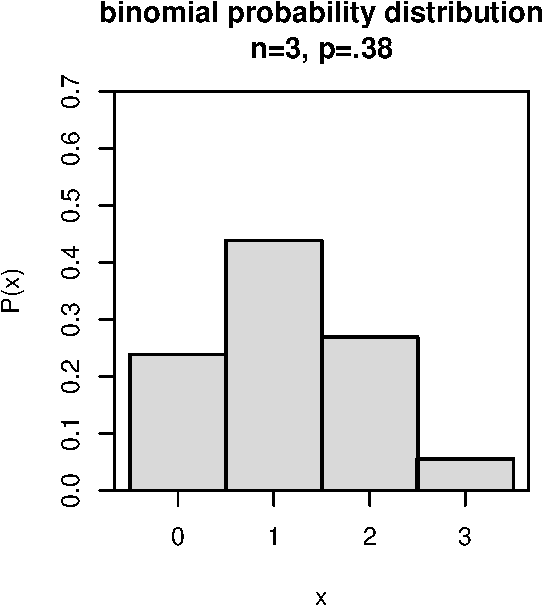
\includegraphics{QMS-EN_files/figure-latex/binomprobabilitydistribution3-1.pdf}
\caption{\label{fig:binomprobabilitydistribution3}Probability distribution of a binomial variable with \(n=3\) and \(p=.38\).}
\end{figure}

We call the probability distribution of a binomial variable the binomial
probability distribution, also referred to as the binomial distribution.
You can calculate the precise probabilities of the binomial
probability distribution with the formula \eqref{eq:prob-binomial} below.

\hypertarget{formulas}{%
\subsection{formulas}\label{formulas}}

The probability of an \(x\) number of hits in \(n\) draws is given as
\begin{equation}
  P(x\,\mbox{hits}) = {n \choose x} p^x (1-p)^{n-x}
  \label{eq:prob-binomial}
\end{equation}
in which \(n\) is the number of draws or attempts, \(x\) is the number of hits
(between 0 and \(n\)), and \(p\) is the probability of a hit.

The coefficient \({n \choose x}\) indicates the number of different orderings
in which we can choose a combination (syllable) of \(x\) elements from\\
\(n\). With \(x=1\) vowel from \(n=3\) draws, there are three possibilities:
one vowel might have been drawn in the first draw, or the second
draw, or the third draw, see
Table \ref{tab:vowelprobabilities}. The number of different possible
orderings is indicated as\\
\begin{equation}
  {n \choose x} = \frac{n!}{x!(n-x)!}
  \label{eq:choose}
\end{equation}
in which
\(x! = x (x-1) (x-2) \dots \times 2 \times 1\), thus
\(4!=4\times3\times2\times1=24\).

\begin{center}\rule{0.5\linewidth}{0.5pt}\end{center}

\begin{quote}
\emph{Example 10.5:} There are 4 chairs for 2 persons. A maximum of 1 person is
allowed to sit down on one chair. How many different orderings of \(x=2\) persons
are possible over \(n=4\) chairs?
\end{quote}

\begin{quote}
Answer: There are
\({4 \choose 2} = \frac{4\times3\times2\times1}{2\times1\times2\times1} = \frac{24}{4} = 6\)
possible orderings, namely 1100, 1010, 1001, 0110, 0101, and 0011.
\end{quote}

\begin{center}\rule{0.5\linewidth}{0.5pt}\end{center}

These binomial coefficients indicating the number of different
possible orderings can quickly be retrieved from Pascal's so-called
triangle, depicted in Table \ref{tab:pascaltriangle}.
We can find the number of different
orderings of \(x=2\) persons over \(n=4\) chairs in row \(n=4\).
The uppermost row is that for \(n=0\). The fifth row is that for \(n=4\) and we
can see the binomial coefficients for \(x= 0, 1, 2, 3, 4\) there one after another.
For \({4 \choose 2}\), we find there the binomial coefficient \(6\).
Every coefficient is the total of the two coefficients above\footnote{Thus, \({n \choose x} = {n-1 \choose x} + {n-1 \choose x-1}\) \citep{Weis15}.}, and
every coefficient can be understood as the number of possible
routes descending from the top of the triangle
to the cell.

\begin{longtable}[]{@{}llllllllclllllll@{}}
\caption{\label{tab:pascaltriangle} Pascal's triangle: Binomial coefficients for the
number of possible orderings for a combination of \(x\) elements from \(n\) (see text).}\tabularnewline
\toprule
\endhead
\(n= 0\): & & & & & & & & 1 & & & & & & &\tabularnewline
\(n= 1\): & & & & & & & 1 & & 1 & & & & & &\tabularnewline
\(n= 2\): & & & & & & 1 & & 2 & & 1 & & & & &\tabularnewline
\(n= 3\): & & & & & 1 & & 3 & & 3 & & 1 & & & &\tabularnewline
\(n= 4\): & & & & 1 & & 4 & & 6 & & 4 & & 1 & & &\tabularnewline
\(n= 5\): & & & 1 & & 5 & & 10 & & 10 & & 5 & & 1 & &\tabularnewline
\(n= 6\): & & 1 & & 6 & & 15 & & 20 & & 15 & & 6 & & 1 &\tabularnewline
\(n= 7\): & 1 & & 7 & & 21 & & 35 & & 35 & & 21 & & 7 & & 1\tabularnewline
\bottomrule
\end{longtable}

The mean and the standard deviation of the binomial probability distribution
are \[\begin{aligned}
    \mu & = & np \\
    \sigma & = & \sqrt{ np(1-p) }\end{aligned}\]

\begin{center}\rule{0.5\linewidth}{0.5pt}\end{center}

\begin{quote}
\emph{Example 10.6:}
The binomial probability distribution for \(x\) hits from \(n=3\) draws with
\(p=.38\) probability of a hit is shown in
Figure \ref{fig:binomprobabilitydistribution3}. This binomial probability
distribution has an average \(\mu=n \times p = 3 \times .38 = 1.14\), and a
standard deviation
\(\sigma = \sqrt{n \times p \times (1-p)} = \sqrt{ 3 \times .38 \times .62} = 0.84\)\textgreater{}
\end{quote}

\begin{center}\rule{0.5\linewidth}{0.5pt}\end{center}

\hypertarget{r-4}{%
\subsection{R}\label{r-4}}

\begin{Shaded}
\begin{Highlighting}[]
\KeywordTok{dbinom}\NormalTok{( }\DecValTok{0}\OperatorTok{:}\DecValTok{3}\NormalTok{, }\DataTypeTok{size=}\DecValTok{3}\NormalTok{, }\DataTypeTok{prob=}\NormalTok{.}\DecValTok{38}\NormalTok{ )}
\end{Highlighting}
\end{Shaded}

\begin{verbatim}
## [1] 0.238328 0.438216 0.268584 0.054872
\end{verbatim}

The output is shown in Table \ref{tab:binomprobabilitydistribution3} below.

\begin{Shaded}
\begin{Highlighting}[]
\NormalTok{matrixcalc}\OperatorTok{::}\KeywordTok{pascal.matrix}\NormalTok{( }\DecValTok{10}\NormalTok{ ) }\CommentTok{\# left under diagonal is Pascal\textquotesingle{}s triangle}
\end{Highlighting}
\end{Shaded}

\begin{verbatim}
##       [,1] [,2] [,3] [,4] [,5] [,6] [,7] [,8] [,9] [,10]
##  [1,]    1    0    0    0    0    0    0    0    0     0
##  [2,]    1    1    0    0    0    0    0    0    0     0
##  [3,]    1    2    1    0    0    0    0    0    0     0
##  [4,]    1    3    3    1    0    0    0    0    0     0
##  [5,]    1    4    6    4    1    0    0    0    0     0
##  [6,]    1    5   10   10    5    1    0    0    0     0
##  [7,]    1    6   15   20   15    6    1    0    0     0
##  [8,]    1    7   21   35   35   21    7    1    0     0
##  [9,]    1    8   28   56   70   56   28    8    1     0
## [10,]    1    9   36   84  126  126   84   36    9     1
\end{verbatim}

Pascal's triangle can be found on the left under the diagonal of this matrix.

\hypertarget{sec:normaldistribution}{%
\section{Normal probability distribution}\label{sec:normaldistribution}}

The more the sample size \(n\) increases, the less gradually the binomial probability
distribution will move up, and the more fluid the probability
distribution will become, as is shown in
Figure \ref{fig:binomprobabilitydistribution50n500}.

\begin{figure}
\centering
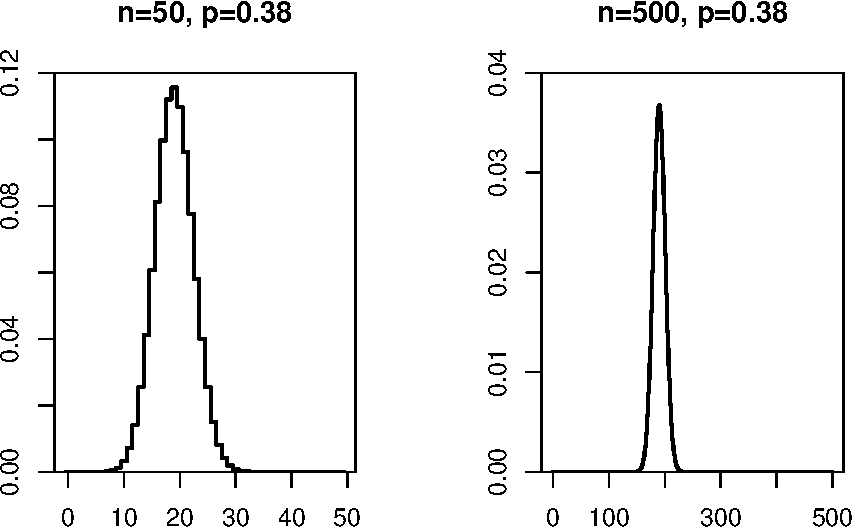
\includegraphics{QMS-EN_files/figure-latex/binomprobabilitydistribution50n500-1.pdf}
\caption{\label{fig:binomprobabilitydistribution50n500}Probability distribution of a binomial variable x with n=50 (left) and n=500 (right) and p=.38.}
\end{figure}

With an even larger sample, the probability distribution becomes a fluid line.
This probability distribution occurs so often, that it is called the
\emph{normal probability distribution} or `normal distribution'. The distribution
is also referred to as the Gaussian distribution (named after the mathematician
Carl Friedrich Gauss, 1777--1855), or the `bell curve' (after the shape). Many
variables approximately follow this probability distribution:
birth weight, body length, vocabulary size, IQ, contents of a 1 litre ℮ carton
of milk, length of a telephone conversation, etc. etc. For all of these variables,
observations close to the average have a high probability of occurring, and
observations which deviate greatly from the average are relatively rare (low
probability).

\begin{figure}
\centering
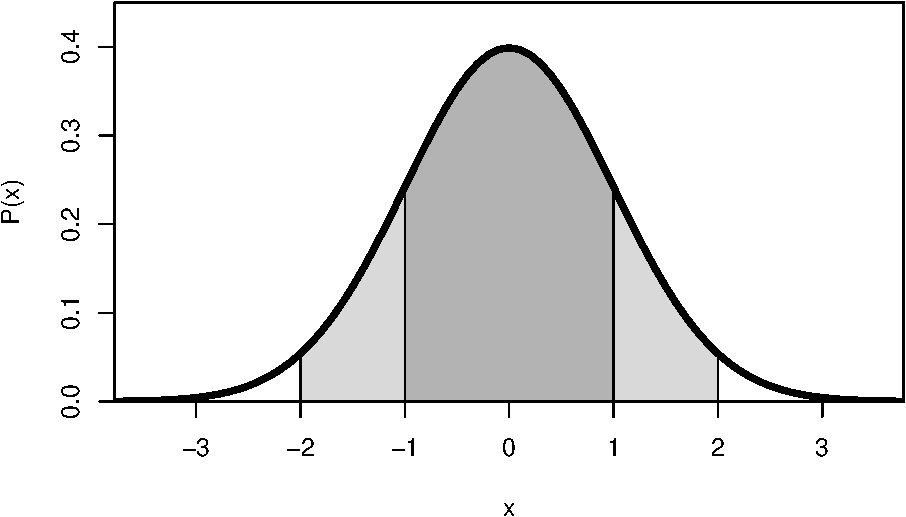
\includegraphics{QMS-EN_files/figure-latex/normalprobabilitydistribution-1.pdf}
\caption{\label{fig:normalprobabilitydistribution}Normal probability distribution of a variable x with average 0 and standard deviation 1.}
\end{figure}

The normal probability distribution of a variable \(X\) with average \(\mu\) and
standard deviation \(\sigma\) has the following characteristics (see
Figure \ref{fig:normalprobabilitydistribution}):

\begin{itemize}
\item
  the distribution is symmetrical around the average \(\mu\),
\item
  the distribution is asymptotic, i.e.~the tails go on infinitely,
\item
  the average, the median and the mode coincide,
\item
  the total area under the curve, i.e.~the total probability of one of
  the possible outcomes, is equal to 1,
\item
  the area under the curve indicates the probability of a value of \(X\) within a
  certain interval,
\item
  the inflection points of the curve (from concave to convex and vice versa) are
  at \(X=\mu-\sigma\) and \(X=\mu+\sigma\),
\item
  around 2/3's of the observations are
  between \(X=\mu-\sigma\) and \(X=\mu+\sigma\) (dark grey area;
  \(P(-1<x/\sigma<1)=.6827\) or 68\%) and around 95\% of the observations are
  between \(-2\sigma\) and \(+2\sigma\) (dark grey plus light grey
  areas; \(P(-2<x/\sigma<2)=.9546\)), this is known as the
  Empirical Rule.
\end{itemize}

A normal probability distribution with \(\mu=0\) and \(\sigma=1\) is referred to as
the standard normal probability distribution. Just as we saw earlier
(§\ref{sec:standardscores}), we can standardise a normally distributed
variable \(x\), i.e.~transform the observations to a standard score
or \(z\)-score: \(z = (x-\overline{x})/s\).
The probability distribution in
Figure \ref{fig:normalprobabilitydistribution} is that of the standard normal
probability distribution of \(Z\), or the probability distribution of \((X-\mu)/\sigma\).

You could calculate the probability distribution of a normally distributed
variable \(X\) yourself with the help of the formula
\eqref{eq:prob-normal} below. However, it is more convenient to
use a table for it; this can be found in
Appendix \ref{app:criticalZvalues}.
Explained in graphical form, the tables provide you, for
different areas or probabilities \(p\) on the right-hand side under the curve,
the positive value of \(Z^*\) which constitutes the left-hand limit of the area.
This means that you have precisely probability \(p\) of finding
a value \(Z\) which is as large as or larger than this lower limit \(Z^*\)
(provided of course that the variable is indeed normally distributed).

\begin{center}\rule{0.5\linewidth}{0.5pt}\end{center}

\begin{quote}
Example 10.7: On the right-hand side of Figure
\ref{fig:normalprobabilitydistribution}, we can see a small white area
under the curve. This area renders the probability that
\(Z>2\). The area has a size of 0.0228. The probability of finding a value of \(Z>2\) is thus 0.0228 or a little less than 2.5\%. (Tip: relate this
probability to the aforementioned Empirical Rule).
\end{quote}

\begin{center}\rule{0.5\linewidth}{0.5pt}\end{center}

In Appendix \ref{app:criticalZvalues}, you can find for convenience not one but two
tables, each consisting of several column designations and
and a row of cells. The first table provides you, for different `rounded'
probabilities \(p\) (columns), the critical values \(Z^*\) (cells), for which the
probability \(p\) of finding a value of \(Z\) which is as large as or larger
than the critical value \(Z^*\), is precisely equal to the value \(p\)
at the top of the column. The second table works the same, but in the case the
`rounded' values of \(Z^*\) are in the cells, and precise probabilities \(p\) are in the
column designations.

What is the probability \(p\) that \(Z>1\)? In the second subtable, second column,
we find \(p=0.1587\). Based on this, we also know that \(P(Z<1)\) must be
\(1-0.1587=0.8413\). Moreover, we know that the distribution is symmetric
(see above), so we know that \(P(Z< -1)\) must also be \(.1587\).
What is the probability \(p\) that \(Z>3\)? In the second subtable, we find
for boundary value \(Z^*=3\) the p-value
\(p=0.0013\). Thus, for a normally distributed variable \(Z\)
there is a p-value \(p=0.0013\) of finding a value of \(Z\)
which is at least three standard variations above the average.

We often want to know the opposite: when we choose a certain p-value,
what should the boundary value \(Z^*\) be?
Which boundary value distinguishes the highest 5\% of observations from the
lowest 95\% (\(p=0.05\))? In the first subtable, we find for p-value
\(p=0.05\) the boundary value \(Z^*=1.645\). This boundary value, calculated back
to the original variable, is often referred to as the 95th percentile or
`P95' of the distribution. Whoever has achieved at least this score,
is part of the top 5\% and has thus performed better than
95\% of the participants
(provided again that the variable is indeed normally distributed).

\begin{center}\rule{0.5\linewidth}{0.5pt}\end{center}

\begin{quote}
\emph{Example 10.8:}
By definition, extreme values occur infrequently with a normally distributed
variable. But what is the limit for an extreme value. Let us assume that
we want to consider no more than 5\% of all observations as extreme.
The normal probability distribution is symmetric, thus from this 5\% we can
expect that one half (2.5\%) is at the left extremity of the distribution,
and the other 2.5\% is on the right-hand side. Which boundary value \(Z^*\)
corresponds with this p-value \(p=0.025\)?
\end{quote}

\begin{quote}
In
Appendix \ref{app:criticalZvalues}, we take the first subtable. In the column
for p-value \(p=0.025\), we find boundary value
\(Z^*=1.960\). If we find an observation with \(Z \ge 1.960\) or with
\(Z \le -1.960\), then we consider that to be an extreme, rare
observation.
\end{quote}

\begin{center}\rule{0.5\linewidth}{0.5pt}\end{center}

\begin{quote}
\emph{Example 10.9:}
Intelligence is expressed as an IQ score, a variable with a normal
probability distribution with \(\mu=100\) and \(\sigma=15\). ``Membership of Mensa
is open to persons who have achieved a score within the upper two
percent of the general population on an approved intelligence test that
has been properly administered and supervised''
(\url{www.mensa.org}). What is the minimum IQ score you must
achieve to become a member?
\end{quote}

\begin{quote}
Answer: The 98th percentile from a standard normally distributed
variable is at \(Z^*=+2.0537\), and thus with
\(x=\overline{x}+2.0537 s = 100+30.8 = 130.8\). Rounded upwards, you thus
have to achieve an IQ score of 131 points or higher.
\end{quote}

\begin{center}\rule{0.5\linewidth}{0.5pt}\end{center}

\begin{quote}
\emph{Example 10.10:}
Verify the aforementioned Empirical Rule with the help of
Appendix \ref{app:criticalZvalues}.
\end{quote}

\begin{center}\rule{0.5\linewidth}{0.5pt}\end{center}

\hypertarget{formulas-1}{%
\subsection{formulas}\label{formulas-1}}

If variable \(X\) has a normal probability distribution, with average \(\mu\)
and standard deviation \(\sigma\), then this is shown as
\begin{equation}
  X \sim \mathcal{N}(\mu,\sigma)
  \label{eq:normallydistributed}
\end{equation}

The normal probability distribution of variable \(X\) with average \(\mu\) and
standard deviation \(\sigma\) is
\begin{equation}
  P(X) = \frac{1}{\sigma \sqrt{2\pi}} \mbox{e}^{ \frac{-(X-\mu)^2}{2\sigma^2} }.
  \label{eq:prob-normal}
\end{equation}

The standard normal probability distribution of variable \(Z\) with average
\(\mu=0\) and standard deviation \(\sigma=1\) is
\begin{equation}
    P(Z) = \frac{1}{\sqrt{2\pi}} \mbox{e}^{ \frac{-Z^2}{2} }
  \label{eq:prob-standardnormal}
\end{equation}

\hypertarget{r-5}{%
\subsection{R}\label{r-5}}

The normal probability distribution in Figure \ref{fig:normalprobabilitydistribution} may be plotted in R using the command below. A \texttt{curve} is plotted, with \texttt{x} in the specified domain, and \texttt{y} being the function which computes the normal probability density using equation \eqref{eq:prob-normal}:

\begin{Shaded}
\begin{Highlighting}[]
\KeywordTok{curve}\NormalTok{( }\KeywordTok{dnorm}\NormalTok{( x, }\DataTypeTok{mean=}\DecValTok{0}\NormalTok{, }\DataTypeTok{sd=}\DecValTok{1}\NormalTok{ ), }\CommentTok{\# function specifying y values, normal density}
       \DataTypeTok{from=}\OperatorTok{{-}}\DecValTok{5}\NormalTok{, }\DataTypeTok{to=}\OperatorTok{+}\DecValTok{5}\NormalTok{, }\CommentTok{\# domain of x}
       \DataTypeTok{lwd=}\DecValTok{4}\NormalTok{, }\CommentTok{\# line width is 4x default value}
       \DataTypeTok{xlab=}\StringTok{"x"}\NormalTok{, }\DataTypeTok{ylab=}\StringTok{"P(x)"} \CommentTok{\# labels along x and y axes}
\NormalTok{       )}
\end{Highlighting}
\end{Shaded}

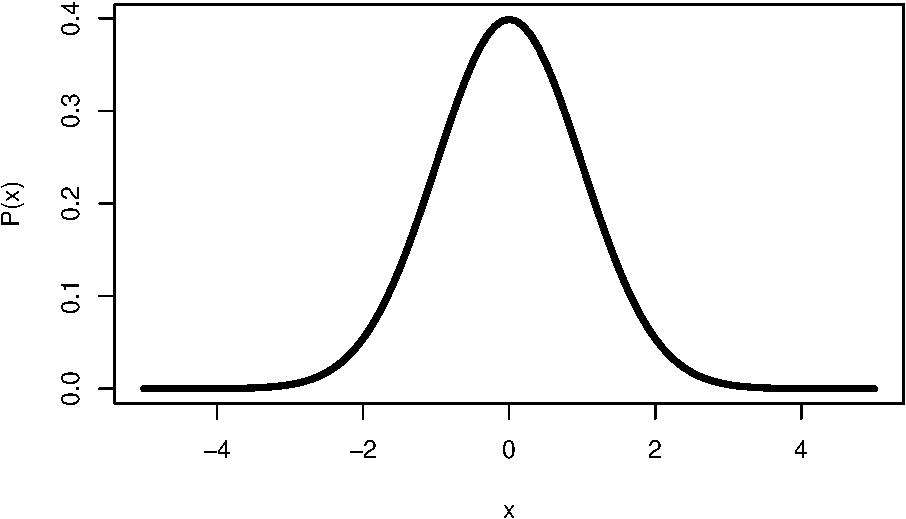
\includegraphics{QMS-EN_files/figure-latex/curve.dnorm-1.pdf}

If used with the additional argument \texttt{curve(\ ...,\ add=TRUE\ )}, then the curve will be added to the most recent plot (see e.g.~Figure \ref{fig:itunesmeanshist} below).

\hypertarget{sec:isvarnormaldistributed}{%
\section{Does my variable have a normal probability distribution?}\label{sec:isvarnormaldistributed}}

The longest song in my digital music library lasts around 50
minutes (it's a piece of classical Indian music, a `morning raga').
A histogram of all music number lengths is shown in
Figure \ref{fig:itunestimeshist}.

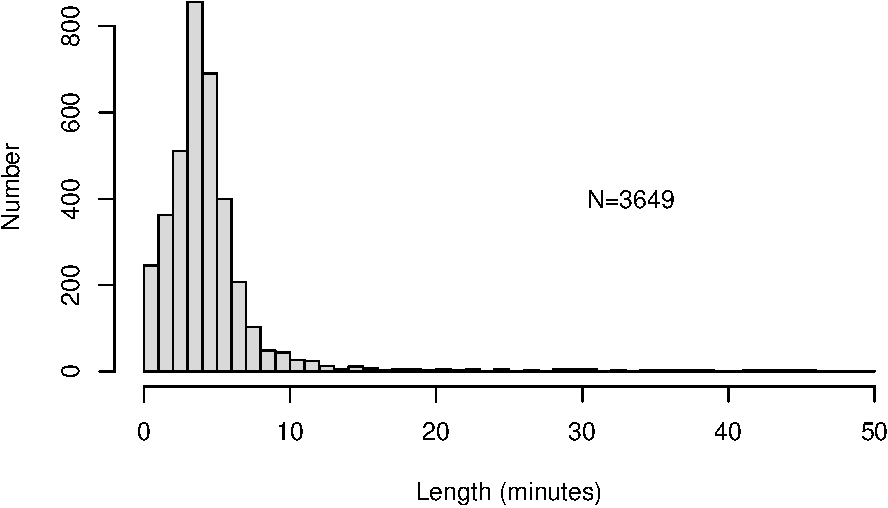
\includegraphics{QMS-EN_files/figure-latex/itunestimeshist-1.pdf}
This histogram shows that these lengths clearly
do \emph{not} follow a normal probability distribution: the distribution is not
symmetric, and the lowest tail does not go on infinitely (there are
no music numbers with negative lengths).

The average \(\bar{x} =\) 4.698 and
standard deviation \(s =\) 5.11 also
point to a non-normal probability distribution:
with a normal distribution, we expect that only \((68/2)+50=84\)\% of the lengths
last longer than
\(\bar{x}-s\approx 0\) minutes, but in reality 100\% last longer
than 0 minutes (thus a larger proportion than expected).

A frequently used technique to inspect whether or not a variable \(X\) has a
normal probability distribution, is to make a graph with the
observed values along one of the axes (here the horizontal axis), and the
corresponding
\(z\)-scores
along the other axis. A figure like this is called a quantile-quantile plot or
Q-Q plot; the Q-Q plot for the lengths in my music library are shown in
Figure \ref{fig:itunestimesqqplot}.

\begin{figure}
\centering
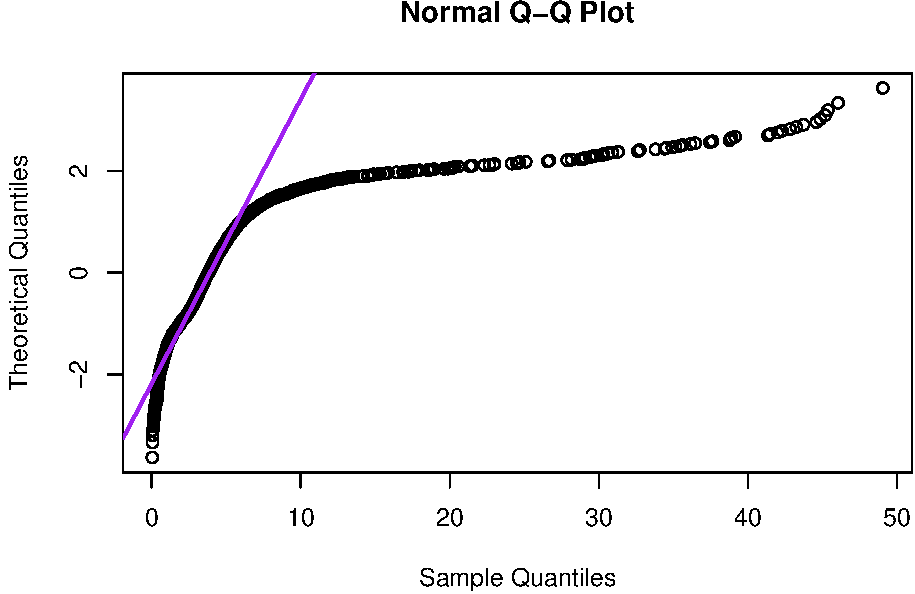
\includegraphics{QMS-EN_files/figure-latex/itunestimesqqplot-1.pdf}
\caption{\label{fig:itunestimesqqplot}Quantile-quantile plot of the lengths of music numbers in my digital library.}
\end{figure}

If the lengths had a normal probability distribution (were normally
distributed), then the points would cluster around the purple straight line. And there would have to be a number of negative lengths\ldots{} The deviations from the purple straight line in
Figure \ref{fig:itunestimesqqplot} thus indicate that the observed lengths
do not follow a normal probability distribution, as we already saw in the
histogram (Figure \ref{fig:itunestimeshist}).

There are also different statistical tests to investigate whether or not a variable
has a normal probability distribution. The two most used are the
Shapiro-Wilk test (with test statistic \(W\))\\
for normality, and the Kolmogorov--Smirnov test (with test statistic \(D\)) for
normality. Both tests investigate the
H0:\(X\sim\mathcal{N}(\bar{X},s)\) (see
formula \eqref{eq:normallydistributed}).

\hypertarget{spss-4}{%
\subsection{SPSS}\label{spss-4}}

\begin{verbatim}
Analyze > Descriptive Statistics > Explore...
\end{verbatim}

Select the variable Time (drag to the Dependent List panel).\\
Choose the button \texttt{Plots}, and tick \texttt{Normality\ plots\ with\ tests}, which
means `if you make a QQ-plot or Normality plot, you should also then conduct
tests on normality'.
Confirm with \texttt{Continue} and afterwards with \texttt{OK}. The output contains
firstly the results of the Shapiro-Wilks test and the
Kolmogorov-Smirnov test. According to both tests, the probability of finding
this distribution, if H0 is true, is almost null -- see however the
warning in
§@ref(\#sec:plargerthannull)! We thus reject H0 and conclude that
the lengths of music numbers are not normally distributed. After these
test results, there is, amongst others, a Q-Q plot.

\hypertarget{r-6}{%
\subsection{R}\label{r-6}}

\begin{Shaded}
\begin{Highlighting}[]
\NormalTok{itunes \textless{}{-}}\StringTok{ }\KeywordTok{read.table}\NormalTok{( }\DataTypeTok{file=}\StringTok{"data/itunestimes20120511.txt"}\NormalTok{, }\DataTypeTok{header=}\OtherTok{TRUE}\NormalTok{ )}
\CommentTok{\# Size in bytes, Time in ms}
\KeywordTok{qqnorm}\NormalTok{(itunes}\OperatorTok{$}\NormalTok{Time}\OperatorTok{/}\DecValTok{60000}\NormalTok{, }\DataTypeTok{datax=}\NormalTok{T, }\DataTypeTok{plot.it=}\OtherTok{FALSE}\NormalTok{) }\CommentTok{\# normally we\textquotesingle{}d use plot.it=TRUE  }
\CommentTok{\# qqline(itunes$Time/60000, datax=T, col="purple", lwd=T) \# see QQ{-}plot above}
\end{Highlighting}
\end{Shaded}

\begin{Shaded}
\begin{Highlighting}[]
\KeywordTok{shapiro.test}\NormalTok{(itunes}\OperatorTok{$}\NormalTok{Time}\OperatorTok{/}\DecValTok{60000}\NormalTok{)}
\end{Highlighting}
\end{Shaded}

\begin{verbatim}
## 
##  Shapiro-Wilk normality test
## 
## data:  itunes$Time/60000
## W = 0.50711, p-value < 2.2e-16
\end{verbatim}

According to this test, the probability of finding a distribution, if H0 is
zero, is almost null, namely smaller than \(2.2 \times 10^{-16}\) (i.e.~smaller than
the smallest number that the analysis packet can render). We therefore
reject H0 and conclude that the length of music numbers is not normally
distributed.

\hypertarget{sec:whatifnotnormal}{%
\section{What if my variable is not normally distributed?}\label{sec:whatifnotnormal}}

In Part III, we will discuss various statistical tests.
The tests which we discuss in Chapters \ref{ch:testing} and \ref{ch:power} and
\ref{ch:anova} however require that the independent
variable has a normal probability distribution. If a variable does \emph{not} have
a (approximately) normal probability distribution, then the variable cannot
simply be used for statistical testing with the statistical tests
there, or to be more precise, the conclusions from such a statistical testing
are not valid then. What can be done? There are then two
possibilities.

Firstly, it is possible to transform the dependent variable \(y\),
i.e.~to apply an arithmetic operation to it. If all is well, that results
in a variable \(y'\) which is actually normally distributed. Much used transformations are: to take the logarithm (\(y'=\log{y}\)), take the square root, or
invert (\(y'=1/y\)). Then, the transformed dependent variable \(y'\) is used for
the statistical testing. Of course, it is imperative to check whether the
new dependent variable \(y'\) is indeed (approximately) normally distributed. When
interpreting the results of the analysis, you should also take into account
the transformation performed!

Secondly, it is sometimes possible to use another statistical test which does
not require that the dependent variable is normally distributed. Those are called
nonparametric tests. We will look at these in more detail in the chapters
\ref{ch:chi-square-tests} and
\ref{ch:other-nonpar-tests}.
A disadvantage of those tests is nevertheless that they have less
statistical power (for a discussion of power,
see Chapter \ref{ch:power}): they are less sensitive, and thus require larger
samples to establish an effect.

\hypertarget{sec:Centrallimittheorem}{%
\section{Probability distribution of average}\label{sec:Centrallimittheorem}}

In this section, we consider the music numbers in my digital
music library as a \emph{population}. We now take a random
sample of \(n=\) 50 numbers, and determine the average length of these
50 music numbers in the sample:
let us say \(\bar{x} =\) 4.401 minutes. Surprisingly
enough, the average of this sample is close to the average
of the population (\(\mu =\) 4.615, see above).
We repeat this operation
\(250\times\): in this way, we get 250 sample averages. The
frequency distribution of these 250 sample averages are shown in
Figure \ref{fig:itunesmeanshist}.

\begin{figure}
\centering
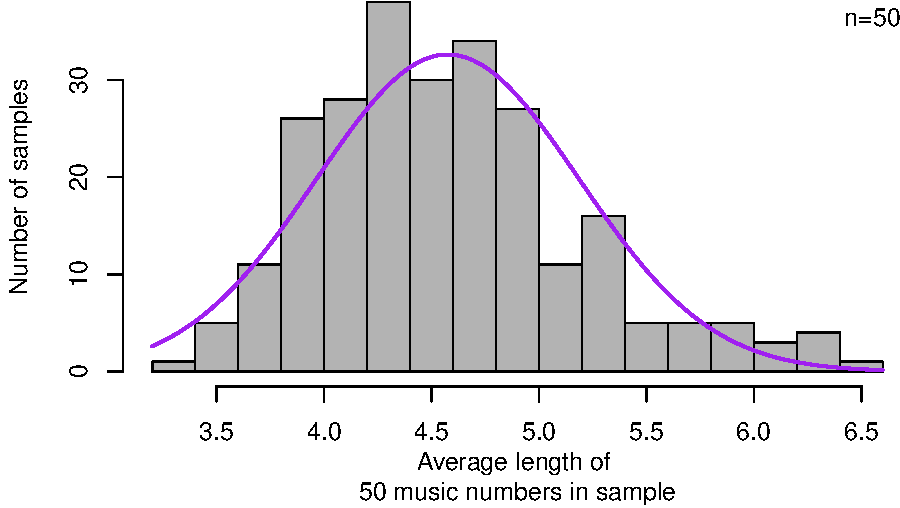
\includegraphics{QMS-EN_files/figure-latex/itunesmeanshist-1.pdf}
\caption{\label{fig:itunesmeanshist}Frequency distribution of 250 averages, each over a random sample of \(n=50\) music numbers (the dependent variable is the length of a music number, in minutes). The matching normal distribution is shown as a fluid curve.}
\end{figure}

Surprisingly enough, these \emph{averages} from (the dependent variables
\(X\) in) the samples \emph{do} show a more or less normal probability distribution,
regardless of whether the variable \(X\) in the population is normally distributed or
not. Put otherwise, the probability distribution of a sample average \emph{always}
approximates the normal probability distribution, regardless of the probability
distribution of the variable in question in the population, provided that the sample
was sufficiently large. (This is known as the Central Limit Theorem). Reread the
above sentences again carefully. As a rule of thumb, the size of the sample, \(n\),
should be at least 30. The larger the sample is, the less the probability
distribution of the sample averages deviates from the normal distribution.

The normal probability distribution of the sample averages has its own average,
\(\mu_{\bar{X}}\), and its own standard deviation,
\(s_{\bar{X}}\). For this, the following applies:
\begin{equation}
    \mu_{\bar{X}} = \mu_X
    \label{eq:meanofmean}
\end{equation}
and
\begin{equation}
    s_{\bar{X}} = \frac{s}{\sqrt{n}}
    \label{eq:sem}
\end{equation}
The standard deviation of the
mean, \(s_{\bar{X}}\), is also known as the `standard error of
the mean'. The same averages \(\bar{X}\) have less dispersion than the separate
observations \(X\), and the averages also vary less when taken over a larger
sample, as seems to be the case from formula \eqref{eq:sem}. You can consider this
standard error of the mean as the `margin of error' in the estimation
of the population average out of the sample average.

What is special now is that we do not have to draw and analyse 250 repeated
random samples. After all, we know that the sample averages have a normal
probability distribution with
\(\mu_{\bar{X}} = \mu_X\) and \(s_{\bar{X}} = \frac{s}{\sqrt{n}}\). We can
derive the probability distribution of the mean from only one sample of
\(n\) observations, with a sample mean \(\bar{X}\) and one standard
deviation \citep{Cumm12}. Reread this paragraph carefully.

\hypertarget{sec:confidenceinterval-mean}{%
\section{Confidence interval of the mean}\label{sec:confidenceinterval-mean}}

As explained above, we can use the mean of the sample, \(\bar{X}\),
as a good estimate of the unknown mean in the population, \(\mu\). On
the basis of the Central Limit Theorem (§\ref{sec:CentralLimitTheorem}),
we also know that the means of repeated samples (of \(n\) observations) follow a
normal distribution: \(\mu_{\bar{X}} \sim \mathcal{N}(\mu_{X},\sigma/\sqrt{n})\),
and thus that 95\% of these repeated sample means will lie between
\(\mu_{X}-1.96\sigma/\sqrt{n}\) and \(\mu_{X}+1.96\sigma/\sqrt{n}\).
This interval is called the 95\% confidence interval. We know with
95\% confidence that the population mean \(\mu\) lies in this interval
--- provided that \(n\) is sufficiently large, and provided that the standard
deviation, \(\sigma\), is known in the population.

In practice, this last condition is rarely or never satisfied. The
standard deviation in the population is usually not known
and this \(\sigma\) is thus also estimated from the sample. We use
the sample of \(n\) observations not only to estimate \(\mu_X\) but also
to estimate \(\sigma_X\). We can then no longer determine the confidence
interval on the basis of the standard normal probability distribution. Instead,
we use an adapted version of it, the so-called t-distribution
(Figure \ref{fig:tprobabilitydistribution}). This probability distribution of
\(t\) is somewhat broader, i.e.~with a somewhat lower peak and with somewhat
thicker tails than the standard normal probability distribution of \(Z\) in
Figure \ref{fig:normalprobabilitydistribution}. The thought behind this is that
the estimation of \(\mu\) is a bit more uncertain (thus the probability distribution
is wider) since not only \(\mu\) but also the standard error of the mean
(\(s/\sqrt{n}\)) are estimated on the basis of the sample. In both estimations, there
can be deviations which mean that there is somewhat more probability of
finding a mean which deviates from the population mean.
As we have already seen, the larger \(n\) is, the better the estimation of \(\mu\):
the t-distribution then approximates the standard normal probability distribution.

\begin{figure}
\centering
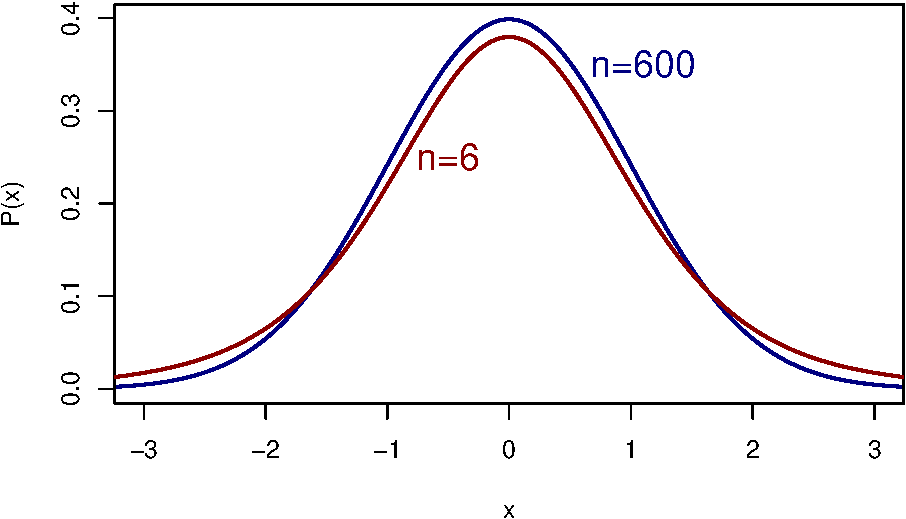
\includegraphics{QMS-EN_files/figure-latex/tprobabilitydistribution-1.pdf}
\caption{\label{fig:tprobabilitydistribution}Probability distribution according to the t-distribution of a variable \(x\) with mean 0 and standard deviation 1, for n=600 and n=6.}
\end{figure}

For the t-distribution, we thus have to know how large the sample was;
after all, this \(n\) determines the precise probability distribution of \(t\),
and with it the critical value \(t*\). We will go into more detail on that
in §\ref{sec:ttest-freedomdegrees}. Here, a detailed example will
suffice.

\begin{center}\rule{0.5\linewidth}{0.5pt}\end{center}

\begin{quote}
\emph{Example 10.11:}
Sometimes a researcher wants to know the speed or tempo with which Dutch is actually spoken,
and how much variation in this speech rate or tempo there is between speakers.
This variable, speech rate, is expressed as the number of seconds
a syllable lasts (typically about \(0.2\) second or \(200\) milliseconds). Although \citet{Quene08}
estimates that \(\mu=0.220\) s and \(\sigma=0.0225\) s, we act as if
we do not know these population parameters --- just like real
researchers who usually do not know
the population parameters.
\end{quote}

\begin{quote}
For a sample of \(n=30\) speakers, we find \(\overline{x}=0.215\)
and
\(s=0.0203\) seconds. From this, we estimate \footnote{Estimations of parameters are indicated with a ``circumflex'' or ``hat'' above them.}
\(\hat{\mu}=0.215\) and
\(\hat{\sigma}=0.0203\). Since \(\sigma\) is not known, we use
the \emph{t}-distribution to determine the confidence interval. We
use the \emph{t}-distribution for \(n=30\) and find a critical value
\(t^*=2.05\) (see Appendix \ref{app:criticaltvalues}, for \(B=95\)\%).
According to formula \eqref{eq:t-onesampleCI}, we know with 95\%
confidence that the unknown population mean \(\mu\) lies
between \(\overline{x}-2.05\times s_{\bar{x}}\) and \(\overline{x}+2.05\times s_{\bar{x}}\),
or between \(0.215-2.05\times0.0037\) and
\(0.215+2.05\times0.0037\),
or between \(0.208\) and \(0.223\) seconds.
If the true value in the population is within these limits, then the observed sample value has a probability of 95\% of occurring \citep[p.241]{Spie19}.
\end{quote}

\begin{center}\rule{0.5\linewidth}{0.5pt}\end{center}

In Figure \ref{fig:tempo95CIs}, you can see the results of a
computer simulation to illustrate this. We have taken \(100\times\)
imaginary samples of \(n=30\) native speakers of Standard Dutch, and established the
speech tempo of these speakers. For each sample, we have drawn
the 95\% confidence interval. For 95 of the 100 samples, the population
mean \(\mu=0.220\) indeed falls within the interval.
But for 5 out of 100 samples, from a population with \(\mu=0.220\), the sample's confidence interval does not contain the population mean (these are marked along the right hand side).

\begin{figure}
\centering
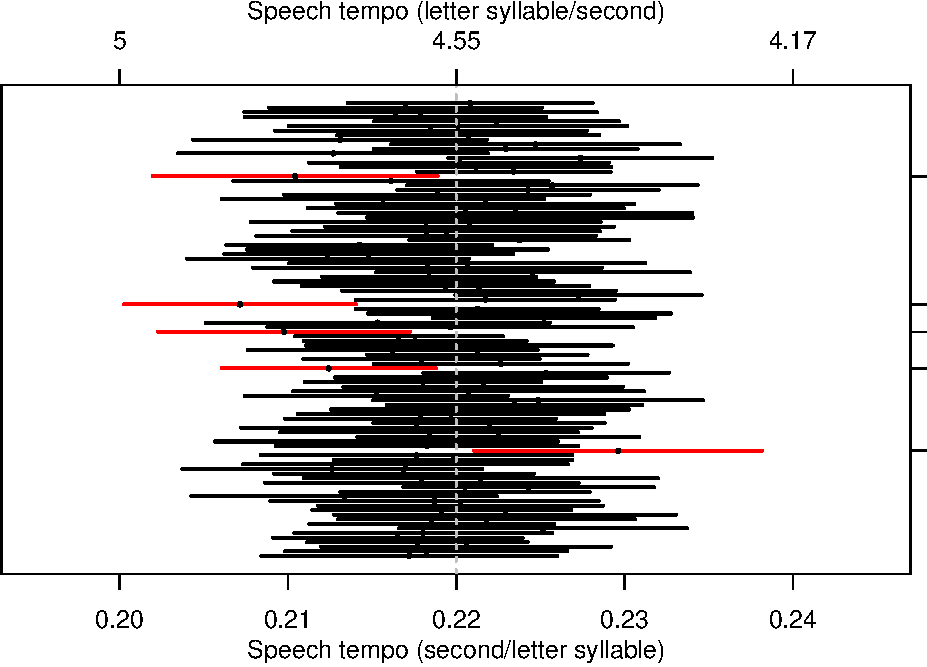
\includegraphics{QMS-EN_files/figure-latex/tempo95CIs-1.pdf}
\caption{\label{fig:tempo95CIs}95\% confidence intervals and sample means, over 100 simulated samples (n=30) out of a population with mean 0.220 and s.d. 0.0225; see text.}
\end{figure}

\hypertarget{formulas-2}{%
\subsection{formulas}\label{formulas-2}}

The two-sided \(B\)\% confidence interval for the population
average is
\begin{equation}
  \bar{X} \pm t^*_{n-1} \times \frac{s}{\sqrt{n}}
  \label{eq:t-onesampleCI}
\end{equation}
in which \(t^*\) with \(n-1\) degrees of freedom is found with the help of
Appendix \ref{app:criticaltvalues}, see
§\ref{sec:ttest-freedomdegrees} for more explanation about this.

\hypertarget{ch:correlation-regression}{%
\chapter{Correlation and regression}\label{ch:correlation-regression}}

\hypertarget{introduction-5}{%
\section{Introduction}\label{introduction-5}}

Most empirical research is focused on establishing associations between
variables. In experimental research, this primarily concerns associations
between independent and dependent variables. In the coming section, we will
look in more detail at the distinct ways of establishing whether a ``significant''
(meaningful, non-accidental) relation exists between
the independent and dependent variables. In addition, the researcher might be
interested in the associations between several dependent variables,
for example the associations between the judgements of several
raters or judges (see also Chapter \ref{ch:reliability}).

In quasi-experimental research, the difference between
independent and dependent variables is usually less clear. Several
variables are observed and the researcher is particularly interested
in the associations between the observed
variables. What, for instance, is the association between the scores for reading,
arithmetic, and geography in the CITO study (see
Table \ref{tab:cito})? In this chapter, we will look in more detail
into the ways of expressing the association in a number:
a correlation coefficient. There are different correlation coefficients depending on
the variable's levels of measurement, which we will
examine more in this chapter.

It is advisable to always first make a graphic representation of
an association between the variables, in the form of a so-called
\emph{scatter plot},
like in Figure \ref{fig:cito-scatter}. Each point in this scatter plot
corresponds with a pupil (or more generally, with a unit from a
sample). The position of each point (pupil) is determined by the observed
values of two variables (here \(X\) is the score for the reading test,
\(Y\) is the score for the arithmetic test). A scatter plot like this helps us to
interpret a potential correlation, and to inspect whether the observations
indeed satisfy the preconditions for calculating a correlation from the
observations. In any case, look at (a) the presence of a potential correlation,
(b) the form of that correlation (linear, exponential,\ldots),
(c) potential outliers (extreme observations, see §\ref{sec:outliers}),
and (d) the distribution of the two variables,
see §\ref{sec:robustefficient}.

\begin{figure}

{\centering 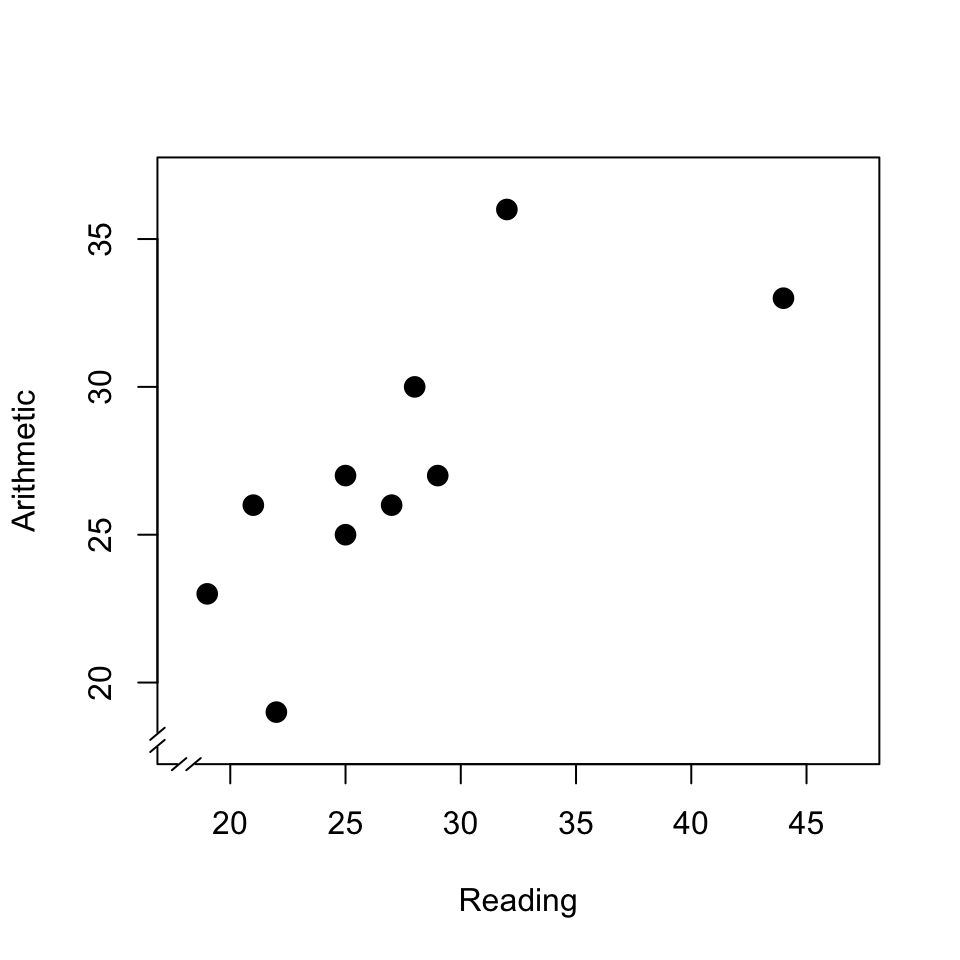
\includegraphics{QMS-EN_files/figure-latex/cito-scatter-1} 

}

\caption{Scatter plot of the scores of a reading test and an arithmetic test; see text.}\label{fig:cito-scatter}
\end{figure}

This scatter plot shows (a) that there is a relation between the scores
for reading and arithmetic. The relation is (b) approximately linear, i.e.
can be described as a straight line; we will return to this in
§\ref{sec:regression}.
The relation also helps us to explain the dispersion in the two
variables. After all, the dispersion in the arithmetic scores can
be partially understood or explained from the dispersion in the reading test:
pupils who achieve a relatively good score in reading, also achieve this
in arithmetic. The observations from the two variables thus not
only provide information about the two variables themselves, but moreover
about the association between the variables. In this scatter plot, we can moreover
see (c) that the highest reading score is an outlier (see also Chapter 9,
Figure \ref{fig:cito-boxplot});
such outliers can have a disproportionately
large influence on the correlation found.

\hypertarget{sec:Pearson}{%
\section{Pearson product-moment correlation}\label{sec:Pearson}}

The Pearson product-moment correlation coefficient is referred to with
the symbol \(r\) (in the case of two variables). This coefficient can be
used if both variables are observed on the interval level of measurement
(§\ref{sec:interval}), and if both variables are approximately
normally distributed
(§\ref{sec:normaldistribution}). Nowadays, we do this calculation
by computer.

For the observations in the scatter plot in
Fig.\ref{fig:cito-scatter}, we can find a correlation of \(r=+.79\). The
correlation coefficient is a number that is by definition between \(-1\)
and \(+1\). A positive correlation coefficient indicates a positive relation:
a larger value of \(X\) corresponds with a larger value
of \(Y\). A negative correlation indicates a negative relation:
a larger value of \(X\) corresponds with a smaller value of
\(Y\). A value of \(r\) which is close to zero indicates a weak
or absent correlation: the dispersion in \(X\) is not related to the
dispersion in \(Y\); there is no or only a weak correlation. We call a correlation of
\(.4<r<.6\) (or \(-.6 < r < -.4\)) moderate. A correlation of
\(r>.6\) (or \(r< -.6\)) indicates a strong association. If \(r=1\) (or
\(r=-1\)), then all observations are precisely on a straight line.
Figure \ref{fig:cor-scatter} shows several scatter plots with the
accompanying correlation coefficients.

\begin{figure}

{\centering 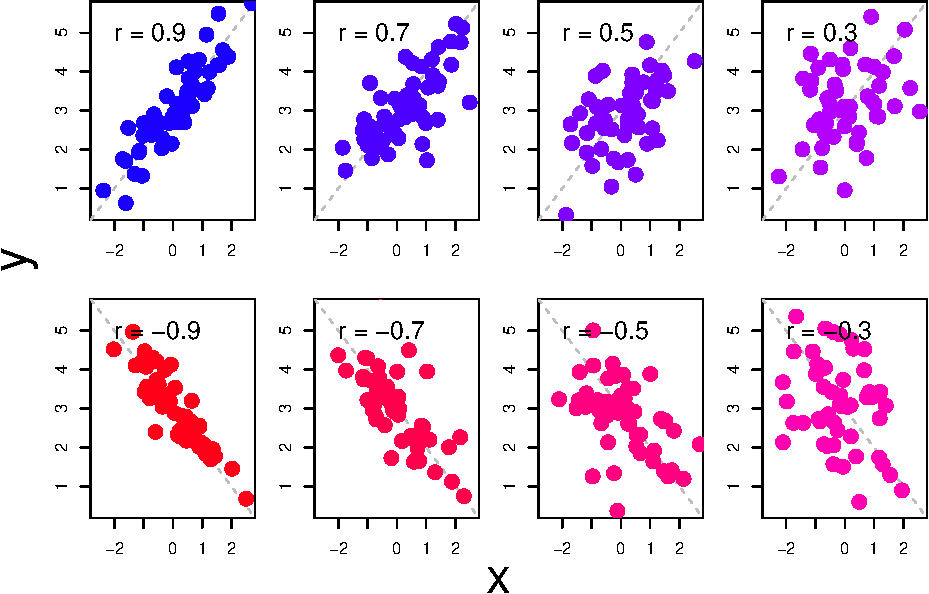
\includegraphics{QMS-EN_files/figure-latex/cor-scatter-1} 

}

\caption{Some scatter plots of observations with accompanying correlation coefficients.}\label{fig:cor-scatter}
\end{figure}

The correlation we see between the scores of the two variables (like
\(r=.79\) between scores for the reading test and arithmetic test,
Fig.\ref{fig:cito-scatter}) might also be the result of
chance variations in the observations. After all, it is possible that
the pupils who have a good score on the reading test achieve
a good score on the arithmetic test purely by chance --- also when there is
actually \emph{not} a correlation between the two variables in the population. We
refer to the unknown correlation in the population with the Greek letter
\(\rho\) (``rho''); as such, it is also possible that \(\rho=0\). Even if \(\rho=0\),
it is possible to have \(n=10\) pupils in the sample who \emph{by chance} combine
high scores on one part with high scores on the other part (and by chance not
have pupils in the sample who combine high scores on one part with low scores
on the other part). We can estimate what the probability \(p\) is
of finding this correlation of \(r=0.79\) or stronger in a sample of
\(n=10\) students, if the association in the population is actually
nil (i.e.~if \(\rho=0\)). We call this probability \(p\) the
\emph{significance} of the correlation coefficient; in Chapter \ref{ch:testing},
we will look in more detail at this term `significance'.
In anticipation of this: if this probability \(p\) is smaller than
\(.05\), then we assume that the correlation found \(r\) is \emph{not by chance},
i.e.~is \emph{significant}. We often see a small probability \(p\) with a strong
correlation \(r\). The correlation coefficient \(r\) indicates the direction
and strength of the relation, and the significance \(p\) indicates the probability
of finding this relation by chance if \(\rho=0\) in the population. We report
these findings as follows\footnote{When the correlation found \(r\) is \emph{not} significant, then this can thus be by chance,
  and then we discount an interpretation of the correlation. We do then state in our report
  the correlation coefficient found and the established significance for it.}:

\begin{center}\rule{0.5\linewidth}{0.5pt}\end{center}

\begin{quote}
\emph{Example 11.1:}
The scores of the \(n=10\) pupils on the CITO test subparts in
Table \ref{tab:cito} show a strong correlation between the scores
on the Reading and Arithmetic tests: Pearson \(r=0.79, p=.007\). Pupils
with a relatively high score on one test generally also achieve
a relatively high score on the other test.
\end{quote}

\begin{center}\rule{0.5\linewidth}{0.5pt}\end{center}

In many studies, we are interested in the correlations between more
than two variables. These correlations between variables are often
reported in a so-called pairwise
correlation matrix like
Table \ref{tab:cito-correlations}, which is a table where the correlations
of all pairs of correlations are reported.

\begin{longtable}[]{@{}lccc@{}}
\caption{\label{tab:cito-correlations} Correlations between the three parts of the CITO
test, as summarised in Table \ref{tab:cito}, with the accompanying significance level between brackets.}\tabularnewline
\toprule
& Reading & Arithmetic & Geography\tabularnewline
\midrule
\endfirsthead
\toprule
& Reading & Arithmetic & Geography\tabularnewline
\midrule
\endhead
Reading & 1.00 & &\tabularnewline
Arithmetic & 0.79 (.007) & 1.00 &\tabularnewline
Geography & -0.51 (.131) & -0.01 (.970) & 1.00\tabularnewline
\bottomrule
\end{longtable}

In this matrix, only the lowest (left) half of the complete
matrix is shown. This also suffices because the cells are mirrored
along the diagonal: after all, the correlation between Reading (column 1) and Arithmetic
(row 2) is the same as the correlation between Arithmetic (row 2) and
Reading (row 1). In the cells on the diagonal, the pairwise correlation matrix
always contains the value \(1.00\), since a variable always correlates perfectly with
itself.
We report these findings as follows:

\begin{center}\rule{0.5\linewidth}{0.5pt}\end{center}

\begin{quote}
\emph{Example 11.2:} The
pairwise correlations between scores from the \(n=10\) pupils on the
three subparts of the CITO test are summarised in
Table \ref{tab:cito-correlations}. We can see a strong correlation between
the scores for the Reading and Arithmetic tests: pupils with a relatively
high score on the Reading test generally also achieve a relatively high
score on the Arithmetic test. The remaining correlations were
not significant.
\end{quote}

\begin{center}\rule{0.5\linewidth}{0.5pt}\end{center}

\hypertarget{formulas-3}{%
\subsection{Formulas}\label{formulas-3}}

The simplest formula for the Pearson product-moment correlation coefficient
\(r\) makes use of the standard normal scores we already used earlier
(§\ref{sec:standardscores}):
\begin{equation}
    r_{XY} = \frac{\sum z_X z_Y}{n-1}
  \label{eq:pearson}
\end{equation}

Just like when we calculate variance
(formula \eqref{eq:variance}), we divide again by
\((n-1)\) to make an estimate of the association in the population.

\hypertarget{spss-5}{%
\subsection{SPSS}\label{spss-5}}

For Pearson's product-moment correlation coefficient:

\begin{verbatim}
Analyze > Correlate > Bivariate...
\end{verbatim}

Choose \texttt{Pearsons} correlation coefficient, tick:
\texttt{Flag\ significant\ correlations}. Confirm \texttt{OK}. The resulting
output (table) does not satisfy the style requirements; as such, you should
take the data into or convert it into a table of your own which does satisfy these requirements.

\hypertarget{r-7}{%
\subsection{R}\label{r-7}}

\begin{Shaded}
\begin{Highlighting}[]
\NormalTok{cito \textless{}{-}}\StringTok{ }\KeywordTok{read.table}\NormalTok{(}\DataTypeTok{file=}\StringTok{"data/cito.txt"}\NormalTok{, }\DataTypeTok{header=}\OtherTok{TRUE}\NormalTok{)}
\CommentTok{\# variable names are Lezen=Reading, Rekenen=Arithmetic, WO=Geography, ...}
\KeywordTok{dimnames}\NormalTok{(cito)[[}\DecValTok{2}\NormalTok{]] \textless{}{-}}\StringTok{ }\KeywordTok{c}\NormalTok{( }\StringTok{"Pupil"}\NormalTok{, }\StringTok{"Reading"}\NormalTok{, }\StringTok{"Arithmetic"}\NormalTok{, }\StringTok{"Geography"}\NormalTok{,}
                          \StringTok{"UrbanRural"}\NormalTok{, }\StringTok{"Arith.2cat"}\NormalTok{ )}
\KeywordTok{cor}\NormalTok{( cito[,}\DecValTok{2}\OperatorTok{:}\DecValTok{4}\NormalTok{] ) }\CommentTok{\# correlation matrix of columns 2,3,4}
\end{Highlighting}
\end{Shaded}

\begin{verbatim}
##               Reading Arithmetic   Geography
## Reading     1.0000000 0.74921033 -0.50881738
## Arithmetic  0.7492103 1.00000000  0.06351024
## Geography  -0.5088174 0.06351024  1.00000000
\end{verbatim}

\begin{Shaded}
\begin{Highlighting}[]
\KeywordTok{with}\NormalTok{( cito, }\KeywordTok{cor.test}\NormalTok{( Reading, Arithmetic ) )}
\end{Highlighting}
\end{Shaded}

\begin{verbatim}
## 
##  Pearson's product-moment correlation
## 
## data:  Reading and Arithmetic
## t = 3.1994, df = 8, p-value = 0.01262
## alternative hypothesis: true correlation is not equal to 0
## 95 percent confidence interval:
##  0.2263659 0.9368863
## sample estimates:
##       cor 
## 0.7492103
\end{verbatim}

\hypertarget{sec:regression}{%
\section{Regression}\label{sec:regression}}

The simplest relation that we can distinguish and describe is a linear
relation, i.e.~a straight line in the scatter plot
(see Fig.\ref{fig:cor-scatter}). This straight line indicates which value
of \(Y_i\) is predicted, on the basis of the value of \(X_i\). This predicted value of
\(Y_i\) is noted as \(\widehat{Y_i}\)
(``Y-hat''). The best prediction \(\widehat{Y_i}\) is based on both the value
of \(X_i\) and the linear relation between \(X\) and \(Y\):
\begin{equation}
    \widehat{Y_i} = a + b {X_i} 
  \label{eq:linearmodel2}
\end{equation}\\
The straight line is described with
two parameters, namely the intercept (or constant) \(a\) and the slope \(b\)
\footnote{In school books, this comparison is described as \(Y = a X + b\), with \(a\) as the slope
  and \(b\) as the intercept; however, we keep to the conventional international notation here.}. The straight line which describes the linear relation is often
referred to as the ``regression line'';
after all, we try to trace the observed values of \(Y\) back to this linear
function of the values of \(X\).

The difference between the observed value \(Y\) and the predicted value
\(\widehat{Y}\) \((Y-\widehat{Y})\) is called the \emph{residual} (symbol
\(e\)). In other words, the observed value is considered to be
the sum of two components, namely the predicted value and the residual:
\begin{align}
    Y   &= \widehat{Y} + e \\
        &= a + b X + e 
  \label{eq:linearmodel3}
\end{align}

The above rationale is illustrated in the scatter plot in
Figure \ref{fig:cito-linearmodel}. The dashed line indicates the linear relation
between the two tests:
\begin{equation}
    \widehat{\textrm{Arithmetic}} = 12.97 + 0.52 \times \textrm{Reading}
  \label{eq:cito-linearmodel}
\end{equation}

\begin{figure}

{\centering 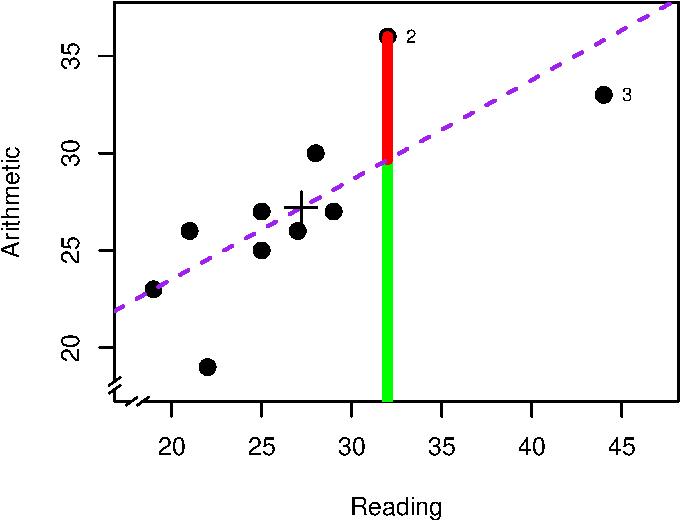
\includegraphics{QMS-EN_files/figure-latex/cito-linearmodel-1} 

}

\caption{Scatter plot of the scores of a reading test and an arithmetic test. The diagram also indicates the regression line (dashed line), the predicted value (green) and residual (red) of the arithmetic test for pupil 2, the average (plus symbol), and markings for pupil 2 and 3; see text.}\label{fig:cito-linearmodel}
\end{figure}

This dashed line thus indicates what the value \(\widehat{Y}\) is for
each value of \(X\). For the second pupil with \(X_2 = 32\),
we thus predict \(\widehat{Y_2} = 12.97 + (0.52) (32) = 29.61\)
(predicted value, green line fragment). For all observations which are not
precisely on the regression line (dashed line),
there is a deviation between the predicted
score \(\widehat{Y}\) and the observed score \(Y\) (residual, red line
fragment). For the second pupil, this deviation is
\(e_2 = (Y_2 - \widehat{Y_2}) = (36-29.61) = 6.49\) (residual, red
line fragment).

As stated, the observed values of \(Y\) are considered to be the
sum of two components, the predicted value \(\widehat{Y}\)
(green) and the residual \(e\) (red). In the same way, the total \emph{variance}
of \(Y\) can be considered to be the sum of the two \emph{variances} of these
components:
\begin{equation}
    s^2_{Y} = s^2_{\widehat{Y}} + s^2_e
  \label{eq:variance-pred-res}
\end{equation}
Of the total variance
\(s^2_Y\) of Y, one part (\(s^2_{\widehat{Y}}\)) can be traced back to and/or
explained from the variance of \(X\), via the linear relation described
with parameters \(a\) and \(b\) (see
formula \eqref{eq:linearmodel2}), and the other part (\(s^2_e\)) cannot be retraced
or explained. The second part, the non-predicted variance of the residuals is also called
the residual variance or unexplained variance.

When we are able to make a good prediction \(Y\) from \(X\), i.e.~when the Pearson
product-moment correlation coefficient \(r\) is high
(Fig. \ref{fig:cor-scatter}, left), then the residuals \(e\) are thus relatively
small, the observations are close around the regression line in the scatter
plot, and then the residual variance \(s^2_e\) is also relatively small.
Conversely, when we are \emph{not} able to predict \(Y\) well from \(X\), i.e.
when the correlation coefficient is relatively low (Fig. \ref{fig:cor-scatter}, right),
then the residuals \(e\) are thus relatively large, the observations are widely dispersed
around the regression line in the scatter plot, and then the residual variance \(s^2_e\) is thus
also relatively large. The square of the Pearson
product-moment correlation coefficient \(r\) indicates what the relative size of the
two variance components is, with respect to the total
variance:
\begin{align}
    r^2 & = \frac{s^2_{\widehat{Y}}}{s^2_Y} \\
        & = 1 - \frac{s^2_e}{s^2_Y}
  \label{eq:r2}
\end{align}
This statistic \(r^2\) is referred to as the ``proportion of explained
variance'' or as the ``coefficient of determination''.

The values of the linear parameters \(a\) and \(b\) in
formula \eqref{eq:linearmodel2} are so chosen that the collective
residuals are as small as possible, i.e.~that the residual variance
\(s^2_e\) is as small as possible (``least squares fit''), and thus \(r^2\)
is as large as possible (see
§\ref{sec:regression-formulas}). In this way, we can find a straight line
which best fits the observations for \(X\) and \(Y\).

A linear regression can also be reported as follows:

\begin{center}\rule{0.5\linewidth}{0.5pt}\end{center}

\begin{quote}
\emph{Example 11.3:}
Based on a linear regression analysis, it appears that the score
for Arithmetic is related to that for Reading: \(b=0.51, r=.79, p_r=.007\), over \(n=10\)
pupils. This linear regression model explains \(r^2=.51\) of the
total variance in the arithmetic scores (the residual standard deviation is
\(s_e= \sqrt{82.803/(n-1-1)} = 3.217\)).
\end{quote}

\begin{center}\rule{0.5\linewidth}{0.5pt}\end{center}

\hypertarget{sec:regression-formulas}{%
\subsection{Formulas}\label{sec:regression-formulas}}

For linear regression of \(y\) on \(x\), we try to estimate the coefficients \(a\)
and \(b\) such that (the square of) the deviation between the predicted value \(\hat{y}\)
and the observed value \(y\) is as small as possible, in other words that the
square of the residuals \((y-\hat{y})\) is as small as possible. This is called the
``least squares'' method (see
\url{http://www.itl.nist.gov/div898/handbook/pmd/section4/pmd431.htm}).

The best estimation for \(b\) is
\[b = \frac{ \sum_{i=1}^n (x_i-\overline{x})(y_i-\overline{y}) } { \sum_{i=1}^n (x_i-\overline{x})^2 }\]

The best estimation for \(a\) is \[a = \overline{y} - b \overline{x}\]

\hypertarget{spss-6}{%
\subsection{SPSS}\label{spss-6}}

For linear regression:

\begin{verbatim}
Analyze > Regression > Linear...
\end{verbatim}

Choose \texttt{Dependent\ variable:\ Arithmetic} and choose
\texttt{Independent\ variable:\ Reading}. Under the button \texttt{Statistics}, tick
\texttt{Model\ fit}, tick \texttt{R\ squared\ change}, choose \texttt{Estimates}, and afterwards
\texttt{Continue}.\\
Under the button \texttt{Plot}, tick \texttt{Histogram} and tick also
\texttt{Normal\ probability\ plot}; these options are required to a get a
numerical (!) summary over the residuals.~
(already check once)
Under the button \texttt{Options}, choose \texttt{Include\ constant} to also have
the constant coefficient \(a\) calculated. Confirm all choices with \texttt{OK}.

The resulting output includes several tables and figures; you cannot
transfer these directly into your report. The table titled \emph{Model
Summary} contains the correlation coefficient, indicated here with capital
letter \(R=.749\).\\
The table titled \emph{Coefficients} contains the regression coefficients. The
line which has the designation \texttt{(Constant)} states coefficient \(a=13.25\);
the line titled \texttt{Reading} states coefficient \(b=0.51\).\\
The table titled \emph{Residual Statistics} provides information about both
the predicted values and the residuals. Check whether the mean of the residual
is indeed null. In this table, we can also see (line 2, column 4) that
the standard variation of the residuals is \(3.212\).

\hypertarget{r-8}{%
\subsection{R}\label{r-8}}

\begin{Shaded}
\begin{Highlighting}[]
\KeywordTok{summary}\NormalTok{( m1 \textless{}{-}}\StringTok{ }\KeywordTok{lm}\NormalTok{( Arithmetic}\OperatorTok{\textasciitilde{}}\NormalTok{Reading, }\DataTypeTok{data=}\NormalTok{cito ) )}
\end{Highlighting}
\end{Shaded}

\begin{verbatim}
## 
## Call:
## lm(formula = Arithmetic ~ Reading, data = cito)
## 
## Residuals:
##     Min      1Q  Median      3Q     Max 
## -5.5332 -1.1167 -0.5332  1.7168  6.3384 
## 
## Coefficients:
##             Estimate Std. Error t value Pr(>|t|)  
## (Intercept)  13.2507     4.4910   2.950   0.0184 *
## Reading       0.5128     0.1603   3.199   0.0126 *
## ---
## Signif. codes:  0 '***' 0.001 '**' 0.01 '*' 0.05 '.' 0.1 ' ' 1
## 
## Residual standard error: 3.406 on 8 degrees of freedom
## Multiple R-squared:  0.5613, Adjusted R-squared:  0.5065 
## F-statistic: 10.24 on 1 and 8 DF,  p-value: 0.01262
\end{verbatim}

The command \texttt{lm} specifies a linear regression model, with \texttt{Arithmetic}
as the dependent variable and \texttt{Reading} as the predictor. This model is
saved as an object called \texttt{m1}, and that is used again directly as an argument
(input) for reporting. In the reporting of model \texttt{m1} the constant coefficient
\(a\) is referred to as the \texttt{Intercept}.

\begin{Shaded}
\begin{Highlighting}[]
\KeywordTok{sd}\NormalTok{( }\KeywordTok{resid}\NormalTok{( m1 ) ) }\CommentTok{\# s.d. of residuals according to \textasciigrave{}m1\textasciigrave{}}
\end{Highlighting}
\end{Shaded}

\begin{verbatim}
## [1] 3.211533
\end{verbatim}

\hypertarget{influential-observations}{%
\section{Influential observations}\label{influential-observations}}

In the previous section, we saw that the aim in a correlation analysis
or regression analysis is for a minimal residual variance.
Earlier we also already saw that outliers or extreme observations, by definition,
make a relatively large contribution to variance. Together, this means that
outliers or extreme observations can have a large influence on the size of
the correlation or on the regression found (the linear relation found). Pupil 3 has an
extremely high score for Reading (see also
Fig.\ref{fig:cito-boxplot}). If we discount pupil 3, then this would not greatly
change the correlation (\(r_{-3}=.79\)) but it would change the slope of the regression line
(\(b=0.84\), more than one and a half times as large as if pupil 3 were in fact included).
This observation thus ``pulls'' hard on the regression line, precisely because
this observation has an extreme value for \(X\) and therefore has much influence.

Non-extreme observations can, however, also have a large influence on the
correlation and regression, if they are far away from the regression line
and thus make a large contribution to the residual variance. This too can be seen in
Fig.\ref{fig:cito-linearmodel}.
Pupil 2 has no extreme scores
but does have the largest residual. If we discounted this pupil 2 then the
correlation would be considerably higher
(\(r_{-2}=.86\)) but the slope of the regression line would only
change a little (\(b=0.45\)).

As such, for a correlation analysis or regression analysis you always have
to make and study a scatter plot in order to see to what extent the results
have been influenced by one or a small number of observations. When doing so, pay
particular attention to observations which are far away from the mean, to each
of the two variables, and to observations which are far away from
the regression line.

\hypertarget{sec:Spearman}{%
\section{Spearman's rank correlation coefficient}\label{sec:Spearman}}

The variables whose correlation we want to investigate
are not always both expressed on the interval level of measurement
(§\ref{sec:interval}), regardless whether or not the researchers
want to and are able to assume that both variables are
approximately normally distributed
(§\ref{sec:normaldistribution}).
In that case, the product-moment correlation is less suitable for
quantifying the association. If the data is indeed expressed on an
ordinal level of measurement, then we can use other correlation coefficients
to express the association: Spearman's rank correlation coefficient
(\(r_s\)) and Kendall's \(\tau\) (the Greek letter ``tau''). Both of these coefficients
are based on the ranking of the observations; we can thus always compute these correlations
when we are able to order the observations. Nowadays, we also perform this calculation
by computer. In this chapter, we only discuss the Spearman's rank correlation
coefficient.

The Spearman's rank correlation coefficient is equal to the Pearson
product-moment correlation coefficient applied to the ranks of
the observations. We convert every observation from a variable to
a rank number, from the smallest observed value (rank 1)
to the largest observed value (rank \(n\)). If two or more observations
have the same value, then they also receive the same
(mean) rank. In
Table \ref{tab:cito-ranks}, you can see the ranks of the scores for Reading
and Arithmetic, ordered here according to the ranks for Reading.

\begin{longtable}[]{@{}lccrccrcccc@{}}
\caption{\label{tab:cito-ranks} Ranks for the scores of 10 pupils on parts of a test, as summarised in
Table \ref{tab:cito}, with difference \(v_i\) between the two ranks per pupil.}\tabularnewline
\toprule
Pupil & 1 & 9 & 6 & 4 & 10 & 8 & 5 & 7 & 2 & 3\tabularnewline
\midrule
\endfirsthead
\toprule
Pupil & 1 & 9 & 6 & 4 & 10 & 8 & 5 & 7 & 2 & 3\tabularnewline
\midrule
\endhead
Reading & 1 & 2 & 3 & 4.5 & 4.5 & 6 & 7 & 8 & 9 & 10\tabularnewline
Arithmetic & 2 & 4 & 1 & 4 & 6.5 & 4 & 8 & 6.5 & 10 & 9\tabularnewline
Difference \(v_i\) & -1 & -2 & 1 & 0.5 & -2 & 2 & -1 & 1.5 & -1 & 1\tabularnewline
\bottomrule
\end{longtable}

The ranking in Table \ref{tab:cito-ranks} makes it clear at a glance that
the three pupils with the lowest score for Reading (nos. 1, 9, 6) also almost achieved
the lowest scores for Arithmetic. That indicates a positive
relation. The two best readers (nos. 2 and 3) are also the two best
arithmeticians. That also indicates a positive relation. However, there is
also no question of a perfect positive relation (thus here \(r_s<1\)), because
then the two rankings would match perfectly.

Think how Table \ref{tab:cito-ranks} would look if there were a perfect
negative relation (\(r_s=-1\)) between the scores for Reading and
Arithmetic, and how the table would look if there were no correlation whatsoever
(\(r_s=0\)) between these scores.

\hypertarget{formulas-4}{%
\subsection{Formulas}\label{formulas-4}}

The association between the rankings of the two variables is expressed
in the Spearman's rank correlation coefficient:
\begin{equation}
    r_s = 1 - \frac{6 \sum v_i^2}{n(n^2-1)}
  \label{eq:spearman}
\end{equation}
in which \(v_i\) stands for
the difference in rankings on both variables for respondent \(i\). The fraction
in this formula gets larger and \(r_s\) thus gets smaller, the larger the
differences between the ranks are.
However, this formula can only be used if there are no ``ties'' (shared rankings) in the
variables; for the dataset in Table \ref{tab:cito-ranks} with ``ties'' in both variables
we have to use another formula.

As can be seen, the Spearman's rank correlation \(r_s\) is not equal to the
Pearson product-moment correlation \(r\) for the scores observed.
If the preconditions of the Pearson coefficient are satisfied, then this
Pearson product-moment correlation coefficient provides a better estimation of the
association than the Spearman's rank correlation coefficient. However, if the preconditions
are \emph{not} satisfied, then the Spearman's coefficient should be preferred again. The
Spearman's coefficient is, amongst others, less sensitive for influential extreme
observations --- after all, such outliers have less weighting once the
raw scores have been replaced by the ranks.

\hypertarget{spss-7}{%
\subsection{SPSS}\label{spss-7}}

For Spearman's rank correlation coefficient:

\begin{verbatim}
Analyze > Correlate > Bivariate...
\end{verbatim}

Choose \texttt{Spearman} rank correlation coefficient, tick:
\texttt{Flag\ significant\ correlations}. Confirm with \texttt{OK}. The resulting
output (table) does not satisfy the style requirements; you thus have to take
the data into or convert it into a table of your own which does satisfy these requirements,
and report according to the usual conventions for correlation analysis.

\hypertarget{r-9}{%
\subsection{R}\label{r-9}}

\begin{Shaded}
\begin{Highlighting}[]
\KeywordTok{with}\NormalTok{(cito, }\KeywordTok{cor.test}\NormalTok{( Reading,Arithmetic, }\DataTypeTok{method=}\StringTok{"spearman"}\NormalTok{ ) )}
\end{Highlighting}
\end{Shaded}

\begin{verbatim}
## Warning in cor.test.default(Reading, Arithmetic, method = "spearman"): Cannot
## compute exact p-value with ties
\end{verbatim}

\begin{verbatim}
## 
##  Spearman's rank correlation rho
## 
## data:  Reading and Arithmetic
## S = 25.229, p-value = 0.00198
## alternative hypothesis: true rho is not equal to 0
## sample estimates:
##       rho 
## 0.8470988
\end{verbatim}

\hypertarget{sec:Phi}{%
\section{Phi}\label{sec:Phi}}

The two variables for which we want to investigate the association are themselves
not always expressed on an ordinal level of measurement (Chapter \ref{ch:levelsofmeasurement}).
Even if both of the variables are measured only on a nominal level of measurement,
then a correlation can still be calculated, namely the phi correlation coefficient
(symbol \(r_\Phi\), with Greek letter ``Phi''). This correlation coefficient can also be used
if one of the two variables is measured on a nominal level of measurement,
and the other one is measured on an ordinal level of measurement.

With our CITO test example, let us assume that the first five
pupils come from a large city (urban), and the last five from the
countryside (rural). The pupil's place of origin is a nominal variable,
with 2 categories, here randomly referred to as \texttt{1} resp. \texttt{0} (see
§\ref{sec:nominal}; a nominal variable with precisely 2
categories is also called a binomial or dichotomous variable).
We now ask ourselves whether there is some association between a
pupil's place of origin and their score for the Arithmetic part of the CITO test.
The second variable is of interval level of measurement. We convert this to a
nominal level of measurement. That can be done in many ways, and it is the
researcher's role to make a wise choice when doing so. Here, we
choose the often used `mean split': one of the categories (low, code \texttt{0})
consists of scores smaller than or equal to the mean
(§\ref{sec:mean}), and the other category consists of scores larger
than the mean (high, code \texttt{1}). We summarise the number of pupils in each of the
\(2\times 2\) categories in a contingency table
(Tabel \ref{tab:cito-contingency-table}).

\begin{longtable}[]{@{}lccc@{}}
\caption{\label{tab:cito-contingency-table} Contingency table of \(n=10\) pupils, subdivided according
to origin (urban=1, rural=0) and according to category of score for the Arithmetic part of
the CITO test (`mean split', low=0, high=1), with letter designations for the number
of observations; see text.}\tabularnewline
\toprule
Origin & Low (0) & High (1) & Total\tabularnewline
\midrule
\endfirsthead
\toprule
Origin & Low (0) & High (1) & Total\tabularnewline
\midrule
\endhead
Rural (0) & 5 (A) & 0 (B) & 5 (A+B)\tabularnewline
Urban (1) & 2 (C) & 3 (D) & 5 (C+D)\tabularnewline
Total & 7 (A+C) & 3 (B+D) & 10 (A+B+C+D)\tabularnewline
\bottomrule
\end{longtable}

The nominal correlation coefficient \(r_\Phi\) is equal to the Pearson
product-moment correlation coefficient applied to the binomial codes
(\texttt{0} and \texttt{1}) of the observations. All 5 pupils from the rural countryside
have an Arithmetic score which is equal to or lower than average
(\(\overline{y}=\) 27.2); out of the pupils from the urban city, 2 have a
score which is (equal to or) lower than average. There is thus an association\\
between the binomial codes of the rows (origin) and those of the columns
(score categories) in Table \ref{tab:cito-contingency-table}.
This association is quantified in the
correlation coefficient \(r_\Phi=0.65\) for this data.

\hypertarget{formulas-5}{%
\subsection{Formulas}\label{formulas-5}}

The nominal correlation coefficient \(r_\Phi\) is calculated as follows,
where the letters refer to the numbers in the cells of a contingency table
(see Table \ref{tab:cito-contingency-table}):
\begin{equation}
    r_\Phi = \frac{(AD-BC)}{\sqrt{(A+B)(C+D)(A+C)(B+D)}}
  \label{eq:phi}
\end{equation}

For the example discussed above we then find
\[
    r_\Phi = \frac{(15-0)}{\sqrt{(5)(5)(7)(3)}} = \frac{15}{22.91} = 0.65
\]

\hypertarget{spss-8}{%
\subsection{SPSS}\label{spss-8}}

The dataset \texttt{cito} already contains the variable \texttt{UrbanRural} which indicates the
origin of the pupils. However, for completeness, we will still show how you can
construct a variable like this for yourself.

\begin{verbatim}
Transform > Recode into different variables...
\end{verbatim}

Choose \texttt{Pupil} as the old variable and fill in as the new name for the new variable
\texttt{UrbanRural2}. Indicate that the old values in \texttt{Range} from
1 to 5 (old) have to be transformed to the new value 1, and likewise that
pupils 6 to 10 have to get the new value 0 for the new variable
\texttt{UrbanRural2}.

For \texttt{Arithmetic} it is a bit more complex. You firstly have to delete
your transformation rules (which relate to \texttt{UrbanRural}). Then, make a new variable
again in the same way as before, named \texttt{Arithmetic2}.
All values from the lowest value to the mean (\(27.2\)) are transformed to the
new value 0 for this new variable. All values
from the mean (\(27.2\)) to the highest value are transformed to the new value 1.

After this preparatory work, we can finally calculate \(r_\Phi\).

\begin{verbatim}
Analyze > Descriptives > Crosstabs...
\end{verbatim}

Select the variables \texttt{UrbanRural2} (in the ``Rows'' panel) and \texttt{Arithmetic2}
(in the ``Columns'' panel) for
contingency table @ref(tab: cito-contingency-table).\\
Choose \texttt{Statistics\ldots{}} and tick the option \texttt{Phi\ and\ Cramer’s\ V}!\\
Confirm firstly with \texttt{Continue} and then again with \texttt{OK}.

\hypertarget{r-10}{%
\subsection{R}\label{r-10}}

The dataset \texttt{cito} already contains a variable \texttt{UrbanRural} which indicates the pupils' origins.
However, for completeness, let us still see how you can construct such a variable for yourself.

\begin{Shaded}
\begin{Highlighting}[]
\NormalTok{UrbanRural2 \textless{}{-}}\StringTok{ }\KeywordTok{ifelse}\NormalTok{( cito}\OperatorTok{$}\NormalTok{Pupil}\OperatorTok{\textless{}}\DecValTok{6}\NormalTok{, }\DecValTok{1}\NormalTok{, }\DecValTok{0}\NormalTok{) }\CommentTok{\# 1=urban, 0=rural}
\NormalTok{Arithmetic2 \textless{}{-}}\StringTok{ }\KeywordTok{ifelse}\NormalTok{( cito}\OperatorTok{$}\NormalTok{Arithmetic}\OperatorTok{\textgreater{}}\KeywordTok{mean}\NormalTok{(cito}\OperatorTok{$}\NormalTok{Arithmetic), }\DecValTok{1}\NormalTok{, }\DecValTok{0}\NormalTok{ ) }\CommentTok{\# 1=high, 0=low}
\end{Highlighting}
\end{Shaded}

Here we build a new variable \texttt{Arithmetic2}, which has the value \texttt{1} if the score for
Arithmetic is higher than the average, and otherwise has the value \texttt{0}.

In R, we also start by making a contingency table (Table \ref{tab:cito-contingency-table} and we then calculate the \(r_\Phi\) over the contingency table.

\begin{Shaded}
\begin{Highlighting}[]
\KeywordTok{print}\NormalTok{( }\KeywordTok{table}\NormalTok{(UrbanRural2,Arithmetic2) {-}\textgreater{}}\StringTok{ }\NormalTok{citocontingencytable ) }
\end{Highlighting}
\end{Shaded}

\begin{verbatim}
##            Arithmetic2
## UrbanRural2 0 1
##           0 5 0
##           1 2 3
\end{verbatim}

\begin{Shaded}
\begin{Highlighting}[]
\CommentTok{\# make and store a contingency table}
\ControlFlowTok{if}\NormalTok{ (}\KeywordTok{require}\NormalTok{(psych)) \{ }\CommentTok{\# for psych::phi}
  \KeywordTok{phi}\NormalTok{(citocontingencytable) }\CommentTok{\# contingency table made earlier is input here!}
\NormalTok{\}}
\end{Highlighting}
\end{Shaded}

\begin{verbatim}
## Loading required package: psych
\end{verbatim}

\begin{verbatim}
## 
## Attaching package: 'psych'
\end{verbatim}

\begin{verbatim}
## The following objects are masked from '.hqenv':
## 
##     harmonic.mean, logit
\end{verbatim}

\begin{verbatim}
## [1] 0.65
\end{verbatim}

\hypertarget{sec:correlationcausation}{%
\section{Last but not least}\label{sec:correlationcausation}}

At the end of this chapter, we want to emphasise again that an association or correlation
between two variables does not necessarily mean
that there is a causal relation between the variables, in other words
a correlation does not mean that one variable (e.g.~treatment) is the consequence of
the other variable (e.g.~cure).
The common saying for this is ``correlation does not imply
causation,'' see also Example 6.1 (Chapter \ref{ch:design})
and accompanying Figure \ref{fig:xkcd552}.

\textbackslash begin\{figure\}

\{\centering 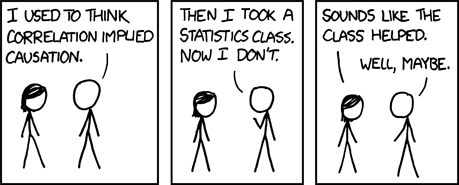
\includegraphics{figures/correlation}

\}

\textbackslash caption\{\emph{Correlation does not imply causation}, borrowed with permission from \url{http://xkcd.com/552}.\}\label{fig:xkcd552}
\textbackslash end\{figure\}

\hypertarget{ch:reliability}{%
\chapter{Reliability}\label{ch:reliability}}

\hypertarget{introduction-6}{%
\section{Introduction}\label{introduction-6}}

In Chapter \ref{ch:validity}, we talked about, amongst other matters,
construct validity, the distance between the intended (theoretical)
concept or construct on the one hand, and the independent or dependent variable
on the other hand. In this Chapter, we will look at another very important
aspect of the dependent variable, namely its \emph{reliability}.
This reliability can be estimated based on the
association between observations of the same construct.
We will also look at the relations between reliability and construct validity.

Often validity and reliability are mentioned in the same breath, and discussed in consecutive
chapters. There is something to be said for this, since both concepts are about how you define and
operationalise your variables. Nevertheless, we have chosen a different ordering here. Reliability
will only be discussed following our discussion of correlation (Chapter
\ref{ch:correlation-regression}), since reliability is based on the relation or correlation
between observations.

\hypertarget{what-is-reliability}{%
\section{What is reliability?}\label{what-is-reliability}}

A reliable person is stable and predictable: what he or she does
today is consistent with what he or she did last week, you can trust
this person --- in contrast to an unreliable person, who
is unstable and behaves unpredictably. According to Collins English Dictionary, someone or something is reliable when they/it ``\ldots can be trusted to work well or to behave in the way that you want them to''.\footnote{\url{https://www.collinsdictionary.com/dictionary/english/reliable}}
Reliable measurements can form the basis for a
``justified true belief'' (see
§\ref{sec:falsification}); conversely, it is not worth
giving credence to unreliable measurements.

Measurements always show some degree of fluctuation or variation or
inconsistency. This variability can partially be attributed to the
variation in the behaviour which is being measured. After all, even if we
measure the same construct for the same person, we still see variance
as a result of the momentary mental or physical state of the participant,
which simply fluctuates. Moreover, there is variation in the measuring device
(thermometer, questionnaire, sensor), and there are probably inconsistencies in the manner
of measurement or evaluation. With the quantification of such consistencies and
inconsistencies, we enter the realms of reliability analysis.

The term `reliability' has two meanings in academic research, which we
will treat separately. Firstly, reliability signifies the \emph{precision}
or \emph{accuracy} of a measurement. This aspect concerns the question of the extent
to which the measurement is influenced by chance factors (through which the
measurement does not exclusively render the construct investigated).
If we do \emph{not} measure
accurately then we also know what the measurements actually show ---
perhaps they show the construct investigated but perhaps they also do not. If we do
measure accurately then we would expect, if we were to conduct the same measurement again,
that we would then measure the same outcome. The less precise a measurement is, the more variation or inconsistency there is between the first measurement and the repeated measurement,
and the measurements are thus less reliable.

\begin{center}\rule{0.5\linewidth}{0.5pt}\end{center}

\begin{quote}
\emph{Example 12.1:} If we want to measure the reading ability
of pupils in their final examinations, then we present them
with a reading comprehension test with a number of accompanying questions.
The degree to which the different questions measure \emph{the same} construct, here the
construct `reading ability', is called reliability, precision or
homogeneity.
\end{quote}

\begin{center}\rule{0.5\linewidth}{0.5pt}\end{center}

In what follows, to avoid confusion, we will refer to this form
of reliability with the term \emph{homogeneity} (vs.~
heterogeneity). With a heterogenous (non-homogenous) test, the total score
is difficult to interpret. With a perfectly homogenous test, people
who have the same total score have also answered the same questions correctly.
However, when we measure human (language) behaviour, such perfectly homogenous tests
never occur: respondents who do achieve the same total score, have not
always answered the same questions correctly (e.g.~in the final examination
reading ability test, Example 12.1). This implies that the questions have not
measured exactly the same capacity. This is also the case: one question was about
paraphrasing a paragraph, whilst another was related to a relationship between
a referential expression and its antecedent.\\
As such, the questions or items were not perfectly homogenous!

Secondly, reliability signifies a measurement's \emph{stability}.
To measure your weight, you stand on a weighing scale. This
measurement is stable: five minutes later, the same weighing scale with the same
person under the same circumstances will also yield (almost)
the same measurement. Stability is often expressed in a so-called
correlation coefficient (a measurement for association, see Chapter
\ref{ch:correlation-regression}). This correlation coefficient can assume all
values between \(+1\) and \(-1\). The more similar the first and second measurement,
the higher the correlation is, and the higher the association between the first and second
measurement. Conversely, the lower the association between the first and second
measurement is, the lower too the correlation is.

Stable measurements nevertheless rarely occur in research on
(language) behaviour. If is a test is taken twice, then there is often
a considerable difference in scores on the first measurement point
and scores on the second measurement point.

\begin{center}\rule{0.5\linewidth}{0.5pt}\end{center}

\begin{quote}
\emph{Example 12.2:}
In the final examination for Dutch secondary school, pupils typically have to write an essay, which is
assessed by two raters. The raters are stable if, after some time, they
give the same judgements to the same essays. Thus: if rater A at first gave a grade
8 to an essay, and for the second evaluation sometime later, he/she also gave the same
essay an 8, then this rater is (very) stable. If, however, the same
rater A gave this same essay a grade 4 on the second evaluation, then this
rater is not stable in his/her judgements.
\end{quote}

\begin{quote}
Now, grading essays is a tricky task: criteria are not precisely described
and there is a relatively large amount of room for
interpretation differences. Accordingly, the stability of judgements is also
low; previously, a stability coefficient of even \(0.40\) has
been reported.
\end{quote}

\begin{center}\rule{0.5\linewidth}{0.5pt}\end{center}

To calculate a test's stability, the same test has to be
taken twice; the degree of association between the first and
second measurement is called the \emph{test-retest-reliability}.
In practice, repeatedly sitting a test like this rarely takes place due to
the relatively high costs and relatively low benefits.

\begin{center}\rule{0.5\linewidth}{0.5pt}\end{center}

\begin{quote}
\emph{Example 12.3:}
\citet{Lata09} developed
a Spanish-language questionnaire consisting of 39 questions, intended
for aphasia patients to determine their quality of life. The quality of life
is described as ``the patient perception about, either the
effects of a given disease, or the application of a certain treatment on
different aspects of life, especially regarding its consequences on the
physical, emotional and social welfare'' \citep[p.379]{Lata09}. The new questionnaire
was taken twice with a sample of 23
Spanish-language patients with aphasia as a result of cerebral haemorrhage.
The reported test-retest stability for this questionnaire was
\(0.95\).
\end{quote}

\begin{center}\rule{0.5\linewidth}{0.5pt}\end{center}

Both homogeneity and stability are expressed as a
coefficient with a value between \(0\) and \(1\) (in practice, negative coefficients
do not occur). How should we interpret the reported
coefficients? Generally, it is of course the case that the higher the coefficient is,
the higher (better) the reliability. But how large should the reliability minimally be
before we can call a test ``reliable''? There are no clear rules for this.
However, when considerations have to be made about people, then the test has to
have a reliability of at least \(0.90\) according to the \emph{Nederlands
Instituut van Psychologen} `Dutch Institute for Psychologists' (NIP).
This is, for instance, the case for tests which are used to determine whether or not a child is eligible for a so-called dyslexia declaration.\\
For research purposes, such a strict requirement for the reliability of a
test is not required. Often, \(0.70\) is used as the lower limit of the
reliability coefficient.

\hypertarget{test-theory}{%
\section{Test theory}\label{test-theory}}

Classical test theory refers to the measurement of variable \(x\)
for the \(i\)-th element of a sample consisting of random members of the
population. Test theory posits that each measurement \(x_i\) is composed
of two components, namely a true score \(t_i\) and an error score:\\
\begin{equation}
  x_i = t_i + e_i
  \label{eq:obs-true-error}
\end{equation}
Imagine that you ``actually'' weigh \(t=72.0\) kg, and imagine also
that your measured weight is \(x=71.6\) kg, then the error score
is \(e=-0.4\) kg.

A first important assumption in classical test theory is that
the deviations \(e_i\) neutralise or cancel each other out (i.e.~are zero when averaged
out, and thus do not deviate systematically from the true score \(t\)), and
that larger deviations above or below occur less often than smaller
deviations. This means that the deviations are normally distributed (see
§\ref{sec:normaldistribution}), with \(\mu_e=0\) as mean:
\begin{equation}
  \label{eq:normal-error}
  e_i \sim \mathcal{N}(0,s^2_e)
\end{equation}

A second important assumption in classical test theory is that there
is no relation between the true scores \(t_i\) and the error scores \(e_i\).
Since the component \(e_i\) is completely determined by chance, and thus does not
have any relation with \(x_i\), the correlation between the true score and
the error score is null:
\begin{equation}
  \label{eq:r-true-error}
  r_{(t,e)} = 0
\end{equation}

The total variance of \(x\) is thus\footnote{\(s^2_{(t+e)} = s^2_t + s^2_e + 2 r_{(t,e)} s_t s_e\), with here \(r_{(t,e)}=0\) according to the formula\eqref{eq:r-true-error}.} equal to the sum of the variance
of the true scores and the variance of the error scores:
\begin{equation}
  \label{eq:var-true-error}
  s^2_x = s^2_t + s^2_e
\end{equation}

When the observed variance \(s^2_x\) proportionately contains much
error variance (i.e.~variance of deviations), then the observed scores
have been determined for the most part by chance deviations. That is of course
undesirable. In a such instance, we say that the observed scores
are not reliable; there is much ``noise'' in the observed scores.\\
When the error variance in contrast is relatively small, then
the observed scores provide a good reflection of what the true scores are,
and then the observed differences are indeed reliable, i.e.~they
are not much determined by chance differences.

In that case, we can also define reliability (symbol \(\rho\)) as the
proportion between true score variance and total variance:\\
\begin{equation}
  \label{eq:rho-reliability}
  \rho_{xx} = \frac{s^2_t}{s^2_x}
\end{equation}

However, in practice, we cannot use this formula \eqref{eq:rho-reliability} to
establish reliability, since we do not know \(s^2_t\). We must thus firstly
estimate what the true score variance is --- or what the error variance is, which, after all,
is the complement of the true score variance (see
formula \eqref{eq:var-true-error})\footnote{An exception to this is a situation in which \(s^2_x=0\), and thus \(s^2_t=0\), thus reliability \(\rho=0\); the dependent variable \(x\) has then not been
  operationalised well.}.

The second assumption (in formula \eqref{eq:r-true-error}), that there is no relation between
true score and error score, is, in practice, not always justified.
To illustrate, let us look at the results of a test on\\
a scale from 1.0 to 10.0. Students with scores of 9 or 10 have a high
true score too (they master the material very well) and thus usually have a low
error score. The students with scores of 1 or 2 also have a low true score
(they master the material very badly) and thus also usually have a low
error score. For the students with scores of 5 or 6,
the situation is different: perhaps they master the material fairly well
but have just given a wrong answer, or perhaps they master the material poorly but have by chance given a good answer. For these students with an observed
score in the middle of the scale, the error scores are relatively larger
than for the students with a score at the ends of the scale. In other domains,
e.g.~for reaction times, we see other relations, e.g.~that the error score increases
more or less equally with the score itself; there is then a positive relationship
between the true score and the error score (\(\rho_{(t,e)}>0\)). Nevertheless,
the advantages of the classical test theory are so large that we use this
theory as a starting point.

From the formulas \eqref{eq:var-true-error} and \eqref{eq:rho-reliability}
above, it also follows that the standard error of measurement is related to the
standard deviation and to the reliability:
\begin{equation}
   \label{eq:standard-error-measurement}
    s_e = s_x \sqrt{1-r_{xx}}
\end{equation}\\
This standard error measurement can be understood
as the standard deviation of the error scores \(e_i\), assuming still that
the error scores are normally distributed (formula \eqref{eq:normal-error}).

\begin{center}\rule{0.5\linewidth}{0.5pt}\end{center}

\begin{quote}
\emph{Example 12.4:}
External inspectors doubt whether teachers mark their students' final
papers well. If a student got a 6, should the final paper have perhaps actually
been judged as a fail?
\end{quote}

\begin{quote}
Let us assume that the given assessment shows a standard deviation
of \(s_x=0.75\), and let us equally assume that an analysis of reliability
had shown that \(r_{xx}=0.9\). The standard error measurement is then \(s_e = 0.24\)
points (rounded up). The probability that the true score \(t_i\) is smaller than
or equal to 5.4 (the minimum for a fail), with an observed
score of \(x_i=6.0\) and \(s_e=0.24\), is only \(p=0.006\) (for explanation,
see §\ref{sec:t-confidenceinterval-mean} below). The
final paper's assessment as a pass is with high probability correct.
\end{quote}

\begin{center}\rule{0.5\linewidth}{0.5pt}\end{center}

\hypertarget{interpretations}{%
\section{Interpretations}\label{interpretations}}

Before we look at the different ways of calculating
reliability, it is a good idea to pause on the different
interpretations of reliability estimations.

First, reliability can be interpreted as the proportion of
true score variance (see formula \eqref{eq:rho-reliability}), or
as the proportion of variance which is ``systematic''.
This is different from the proportion of variance resulting from the concept-as-defined,
the ``valid'' variance (see Chapter \ref{ch:validity}).
The variance resulting from the concept-as-defined is part of the proportion of
true score variance.
However, many other factors may systematically influence
respondents' scores, such as differences in test experience. If two students \(i\) and \(j\)
possess a concept (let us say: language proficiency) to the same degree, then one of the
students can still score more highly because he or she has done (and practiced) language proficiency
tests more often than the other student. Then, there is no difference
in the concept-as-defined (language proficiency \(T_i = T_j\)),\\
but there is in another factor (experience), and thus a difference arises
between the students in their `true' scores (\(t_i \neq t_j\)) which
we measure with a valid and reliable language proficiency measurement. When measuring,
deviations and measurement errors appear (\(e_i\) and \(e_j\)), through which
the observed differences between students (\(x_i-x_j\)) can be larger or smaller than their
differences in `true' score (\(t_i-t_j\)).
This is the reason why a reliability estimate always forms the upper limit of
the validity.

A second interpretation of reliability (formula \eqref{eq:rho-reliability})
is that of the theoretically expected correlation (see
§\ref{sec:Pearson}) between measurements, when measurements are replicated
many times. For convenience, we assume that memory and fatigue
effects have no effect at all on the second and later measurements. If we were to
measure the same people with the same measurement
three times, without memory or fatigue effects, then the scores from the first and
second measurement, and from the first and third measurement, and from
the second and third measurement would always show the same correlation
\(\rho\). This correlation thus indicates the extent to which the repeated measurements
are consistent, i.e.~represent the same unknown true score.

In this interpretation, reliability thus expresses the expected association
between scores from the same test taken repeated times. We then interpret the reliability
coefficient \(\rho\) as the correlation between two measurements
with the same instrument.

Thirdly, reliability can be interpreted as the loss
of efficiency in the estimation of the mean score \(\overline{X}\)
\citep[ p.474]{Ferg89}. Imagine that we want to establish the mean score of a group of
\(n=50\) participants, and for this we use a measurement instrument
with reliability \(\rho_{xx}=0.8\). In this case, there is uncertainty in the estimation,
which come from the chance deviations \(e_i\) in the measurements.
If the measurement instrument were perfectly reliable (\(\rho=1\)), we would only
need \(\rho_{xx}\times n = 0.8\times50=40\) participants for the same accuracy in
the estimation of \(\overline{X}\)
\citep[ p.474]{Ferg89}. As such, we have, as it were, played away 10 participants
to compensate for the unreliability of the measurement instrument.

Above, we spoke about measurements with the help of measurement instruments,
and below we will talk about ratings done
by raters. In these situations, the approach to the notion of `reliability'
is always the same. Reliability plays a role in all situations where
elements from a sample are measured or assessed by multiple assessors or instruments.
Non-final exams and questionnaires can also be such measurement instruments: a non-final
exam or questionnaire can be thought of as a composite instrument
with which we try to measure an abstract property or condition of the participants.
Each question can then be considered as a
``measurement instrument'' or ``assessor'' of the respondent's property or condition.
For this, all of the above mentioned insights and interpretations concerning
test theory, measurement error and reliability are equally applicable.

\hypertarget{methods-for-estimating-reliability}{%
\section{Methods for estimating reliability}\label{methods-for-estimating-reliability}}

A measurement's reliability can be determined in different ways.
The most important are:

\begin{itemize}
\item
  The \emph{test-retest method}\\
  We conduct all measurements twice, and then calculate the correlation
  between the first and the second measurement. The fewer measurement errors
  and deviations the measurements contain, the higher the correlation
  and thus also the reliability is. This method is
  time consuming but can also be applied to a small portion of the
  measurements. In speech research, this method is indeed used to establish
  the reliability of phonetic transcriptions: part of the speech
  recordings are transcribed by a second assessor, and then both transcriptions
  are compared.
\item
  The \emph{parallel forms method}\\
  We have a large collection of measurements which are readily
  comparable and measure the same construct. We conduct all
  measurements repeatedly, the first time by combining the measurements
  of several measurement instruments chosen at random (let's say A
  and B and C) and the second time by using other random
  instruments (let's say D and E and F). Since the measurement instruments are
  `parallel' and the same measurement is considered to be measured, the correlation
  between the first and the second measurement is an indication of the
  measurement's reliability.
\item
  The \emph{split-half method}\\
  This method is similar to the parallel forms method. The \(k\) questions
  or instruments are divided into two halves, after which the score
  is determined within each half. From the correlation \(r_{hh}\) between
  the scores from the two half tests, the reliability of the whole test can
  be deduced, \(r_{xx} = \frac{2r_{hh}}{1+r_{hh}}\).
\end{itemize}

\hypertarget{reliability-between-assessors}{%
\section{Reliability between assessors}\label{reliability-between-assessors}}

As an example, let us look at language proficiency measurements from students
in a foreign language. This construct `language proficiency'
is measured in this example by means of two assessors who each, independently
of the other, award a grade between 1 and 100 to the student (higher is better).
However, when assessing, measurement errors also arise, through which the judgements
not only reflect the underlying true score but also a deviation if it, with
all the aforementioned assumptions. Let us firstly look at the
judgements by the first and second rater (see Table
\ref{tab:reliability}). For the time being, the final judgement of a student is
the mean of the judgements from the first and second rater.

\begin{longtable}[]{@{}cccc@{}}
\caption{\label{tab:reliability} Judgements about language proficiency
from \(n = 10\) students (rows) by \(k = 3\) raters (columns).}\tabularnewline
\toprule
Student & B1 & B2 & B3\tabularnewline
\midrule
\endfirsthead
\toprule
Student & B1 & B2 & B3\tabularnewline
\midrule
\endhead
1 & 67 & 64 & 70\tabularnewline
2 & 72 & 75 & 74\tabularnewline
3 & 83 & 89 & 73\tabularnewline
4 & 68 & 72 & 61\tabularnewline
5 & 75 & 72 & 77\tabularnewline
6 & 73 & 73 & 78\tabularnewline
7 & 73 & 76 & 72\tabularnewline
8 & 65 & 73 & 72\tabularnewline
9 & 64 & 68 & 71\tabularnewline
10 & 70 & 82 & 69\tabularnewline
\(\overline{x_i}\) & 71.0 & 74.4 & 71.7\tabularnewline
\(s_i\) & 5.6 & 7.0 & 4.7\tabularnewline
\bottomrule
\end{longtable}

The judgements of only the first and the second assessor show a
correlation of \(r_{1,2}=.75\). This means (according to the formula
\eqref{eq:rho-reliability}) that 75\% of the total variance in the
judgements of these two raters can be attributed to differences
between the students rated, and thus 25\% of measurement errors (after all,
we have assumed that there are no systematic differences between
raters). The proportion of measurement errors appears to be quite high.
However, we can draw hope from one of our earlier observations, namely that
the raters' measurement errors are not correlated. The
\emph{combination} of these two raters --- the mean score per student
over the two raters --- thus provides more reliable measurements
than each of the two raters can do separately. After all, the
measurement errors of the two raters tend to cancel each other out
(see formula \eqref{eq:normal-error}).
Reread the last two sentences carefully.

Reliability is often expressed as \emph{Cronbach's Alpha}
\citep{Cort93}. This number is a measure for the consistency or homogeneity
of the measurements, and thus also indicates the degree to which the two
raters have rated the same construct. The simplest definition is
based on \(\overline{r}\), the mean correlation between
measurements of \(k\) different raters\footnote{In our example, there are only \(k=2\) raters, thus there is only one
  correlation, and \(\overline{r} = r_{1,2} = 0.75\).}.
\begin{equation}
  \label{eq:cronbach-corr}
  \alpha = \frac{k \overline{r}} {1+(k-1)\overline{r}}
\end{equation}

Filling in \(k=2\) raters and \(\overline{r}=0.75\) provides \(\alpha=0.86\) (SPSS and R
use a somewhat more complex formula for this, and report
\(\alpha=0.84\)). This measurement for reliability is not only referred to
as Cronbach's Alpha but also as the Spearman-Brown formula
or the Kuder-Richardson formula 20 (KR=20)\footnote{The so-called `intra-class correlation coefficient' (ICC) for \(k\)
  is likewise identical to the Cronbach's Alpha.}.

The value of Cronbach's Alpha found is a bit tricky to evaluate
since it is also dependent on the number of instruments or raters or
questions in the test \citep{Cort93, Glin01}. For academic research,
a lower limit of 0.75 or 0.80 is often used. If the result of the test or measurement
is of great importance to the person concerned, as in the case of medical or
psychological patient diagnosis, or when recruiting and selecting personnel, then
an even higher reliability of \(\alpha=.9\) is recommended \citep{Glin01}.

If we want to increase reliability to \(\alpha=0.9\) or higher, then
we can achieve that in two ways. The first way is to expand the
number of raters. If we combine more raters in the total score,
then the measurement errors of these raters also better cancel out each other,
and then the total score is thus more reliable. Using
the formula \eqref{eq:cronbach-corr}, we can investigate how many raters
are needed to improve the reliability to \(\alpha=0.90\) or better. We fill in\\
\(\alpha=0.90\) and again \(\overline{r}=0.75\), and then find an outcome of
minimally \(k=3\) raters. The \emph{increase} in reliability levels off, the more
raters there are already participating: if \(k=2\) then \(\alpha=.84\), if \(k=3\) then
\(\alpha=.84+.06=.90\), if \(k=6\) then \(\alpha=.90+.05=.95\), if \(k=9\) then
\(\alpha=.95+.01=.96\), etc. After all, if there are already 6 raters who are
already readily cancelling out each other's measurement errors, then 3 extra
assessors add little to the reliability.

The second way of increasing reliability is by reducing the measurement
error. We can try to do this, for example, by instructing the raters as well as
possible
about how they should rate the students' language proficiency. An assessment
protocol and/or
instruction can make the deviations between and within raters smaller.
Smaller deviations mean smaller measurement errors, and that again means
higher correlations between the raters. For an
\(\overline{r}=0.8\), we already almost achieve the desired reliability, with
only \(k=2\) raters.

A third way of increasing reliability requires a closer analysis of
the separate raters. To explain this, we also now involve the third
rater in our considerations (see Table
\ref{tab:reliability}). However, the judgements of the third rater show
low correlations with those of the first and second
assessor: \(r_{1,3}=0.41\) and \(r_{2,3}=0.09\). As a consequence, the mean
correlation between assessors is now lower,
\(\overline{r}=0.42\). As a result of taking this third rater, the reliability
has not risen but instead actually lowered to
\(\alpha = \frac{3\times0.42}{1+2\times0.42} = 0.68\). We can thus
perhaps better ignore the measurements of the third rater.
Also if we investigate the reliability of a non-final exam or test or questionnaire
it can seem that the reliability of a whole test \emph{increases} if some
``bad'' questions are removed. Apparently, these ``bad'' questions measured
a construct which differed from what the remaining questions measured.

\hypertarget{reliability-and-construct-validity}{%
\section{Reliability and construct validity}\label{reliability-and-construct-validity}}

When a measurement is reliable, then ``something'' has been measured reliably.
But this still does not show \emph{what} has been measured! There is a
relation between reliability (how measurements are made) and construct
validity (what is measured, see
Chapter \ref{ch:validity}), but these two terms are not identical.
Sufficient reliability is a requirement for validity, but
is not a sufficient condition for it. Put otherwise: a test which
is not reliable can also not be valid (since this test also measures noise),\\
but a test which is reliable does not have to be valid.
Perhaps, the test used does measure another construct other than what
was intended very reliably.

An instrument is construct valid if the concept measured matches
the intended concept or construct. In
Example 12.3, the questionnaire is valid if the score from
the questionnaire matches the quality of life (whatever that actually
is) of the aphasia patients. Only once it has been shown that
an instrument is reliable, is it meaningful to speak about a measurement's
construct validity. Reliability is a necessary but not a sufficient condition for
construct validity. An unreliable
instrument can thus not be valid but a reliable instrument does not necessarily
have to be valid.

To measure reading proficiency, we get the pupils to write
an essay. We count the number of letters \emph{e} in each essay. This is
a very reliable measurement: different raters arrive at the same
number of \emph{e}'s (raters are homogenous) and the same rater always also
delivers the same outcome (raters are stable). The great objection here is that
the number of \emph{e}'s in an essay does not or does not necessarily match the concept
of reading proficiency. A pupil who has incorporated more \emph{e}'s into his/her essay
is not necessarily a better writer.

Whilst researchers know that reliability is a necessary but not
sufficient condition for validity, they do not always use these terms
carefully. In many studies, it is tacitly
assumed that if the reliability is sufficient, the validity
is also then guaranteed. In Example 12.3 too, the difference is not
made clear and
the researchers do not discuss the construct validity of their new
questionnaire explicitly.

\hypertarget{spss-9}{%
\section{SPSS}\label{spss-9}}

For a reliability analysis of the \(k=3\) judgements over
language proficiency in
Table~\ref{tab:reliability}:\\

\begin{verbatim}
Analyze > Scale > Reliability Analysis...
\end{verbatim}

Select the variables which are considered to measure the same construct;
here that is three raters. We look at these \(k=3\)
assessors as ``items'' who measure the property ``language proficiency'' of 10
students. Drag these variables to the Variable(s) panel.\\
As Scale label, fill in an indication of the construct, e.g.
\texttt{language\ proficiency}.\\
As a method, choose \texttt{Alpha} for Cronbach's Alpha (see formula
\eqref{eq:cronbach-corr})\\
Choose \texttt{Statistics\ldots{}}, tick: Descriptives for
\texttt{Item,\ Scale,\ Scale\ if\ item\ deleted}, Inter-Item \texttt{Correlations},
Summaries \texttt{Means,\ Variances}, and confirm with \texttt{Continue} and again
with \texttt{OK}.

The output includes Cronbach's Alpha, the desired inter-item correlations
(particularly high between raters 1 and 2), and (in Table
Item-Total Statistics) the reliability if we remove a certain
rater. This last output teaches us that
raters 1 and 2 are more important than rater 3. If we
were to replace raters 1 or 2, then the reliability would collapse
but if we were to remove rater 3 then the reliability
would even increase (from 0.68 to 0.84). Presumably, this rater
has rated a different concept to the others.

\hypertarget{r-11}{%
\section{R}\label{r-11}}

For a reliability analysis of \(k=3\) language proficiency
judgements in Table \ref{tab:reliability}:\\

\begin{Shaded}
\begin{Highlighting}[]
\NormalTok{raters \textless{}{-}}\StringTok{ }\KeywordTok{read.table}\NormalTok{(}\DataTypeTok{file=}\StringTok{"data/beoordelaars.txt"}\NormalTok{, }\DataTypeTok{header=}\OtherTok{TRUE}\NormalTok{)}
\ControlFlowTok{if}\NormalTok{ (}\KeywordTok{require}\NormalTok{(psych)) \{ }\CommentTok{\# for psych::alpha}
  \KeywordTok{alpha}\NormalTok{( raters[,}\DecValTok{2}\OperatorTok{:}\DecValTok{4}\NormalTok{] ) }\CommentTok{\# columns 2 to 4}
\NormalTok{\}}
\end{Highlighting}
\end{Shaded}

\begin{verbatim}
## Number of categories should be increased  in order to count frequencies.
\end{verbatim}

\begin{verbatim}
## 
## Reliability analysis   
## Call: alpha(x = raters[, 2:4])
## 
##   raw_alpha std.alpha G6(smc) average_r S/N  ase mean  sd median_r
##       0.68      0.68    0.74      0.41 2.1 0.17   72 4.6     0.41
## 
##  lower alpha upper     95% confidence boundaries
## 0.35 0.68 1.01 
## 
##  Reliability if an item is dropped:
##    raw_alpha std.alpha G6(smc) average_r  S/N alpha se var.r med.r
## B1      0.15      0.16   0.088     0.088 0.19    0.497    NA 0.088
## B2      0.58      0.58   0.410     0.410 1.39    0.264    NA 0.410
## B3      0.84      0.85   0.745     0.745 5.84    0.095    NA 0.745
## 
##  Item statistics 
##     n raw.r std.r r.cor r.drop mean  sd
## B1 10  0.93  0.92  0.91   0.81   71 5.6
## B2 10  0.84  0.78  0.72   0.53   74 7.0
## B3 10  0.56  0.64  0.38   0.25   72 4.7
\end{verbatim}

This output includes Cronbach's Alpha (\texttt{raw\_alpha\ 0.68}), and the
reliability if we were to remove a certain rater.
If we were to replace rater 3, then the reliability would even
increase (from 0.68 to 0.84). Over all three raters,
\texttt{average\_r=0.41}.

Correlations between \(k\) raters or items are not explicitly
provided (even if they can be deduced from the above output),
thus we still request these:

\begin{Shaded}
\begin{Highlighting}[]
\KeywordTok{cor}\NormalTok{( raters[ ,}\KeywordTok{c}\NormalTok{(}\StringTok{"B1"}\NormalTok{,}\StringTok{"B2"}\NormalTok{,}\StringTok{"B3"}\NormalTok{) ] ) }\CommentTok{\# explicit column names}
\end{Highlighting}
\end{Shaded}

\begin{verbatim}
##           B1         B2         B3
## B1 1.0000000 0.74494845 0.40979738
## B2 0.7449484 1.00000000 0.08845909
## B3 0.4097974 0.08845909 1.00000000
\end{verbatim}

\begin{center}\rule{0.5\linewidth}{0.5pt}\end{center}

\hypertarget{part-part-iii-inferential-statistics}{%
\part*{Part III: Inferential statistics}\label{part-part-iii-inferential-statistics}}
\addcontentsline{toc}{part}{Part III: Inferential statistics}

\hypertarget{ch:testing}{%
\chapter{Testing hypotheses}\label{ch:testing}}

\hypertarget{sec:testing-introduction}{%
\section{Introduction}\label{sec:testing-introduction}}

From this chapter onwards, we will be concerned with the testing of
research hypotheses and, in particular, with null hypothesis significance testing (NHST),
as explained in Chapter \ref{ch:research}.

Over the course of the years, a large number of techniques have been developed
for tests like this. The tests with which we will concern ourselves
are the most used and can be divided into parametric
and non-parametric tests. Parametric tests assume that the dependent
variable is (at least) measured on an interval level of measurement (see
Chapter~\ref{ch:levelsofmeasurement}), and that the measured outcomes or
scores are normally distributed (see
§\ref{sec:normaldistribution} and §\ref{sec:whatifnotnormal}).
For non-parametric tests, dependent on the technique,
fewer assumptions are made over the level of measurement or over
the distribution of the observed scores; these are so-called
distribution free tests. The consequence is that the testing
is a little less `sensitive' under otherwise equal circumstances, i.e.
that the null hypothesis can be rejected less often in
otherwise equal circumstances. These tests therefore have less power (see
Chapter \ref{ch:power}). Researchers thus usually prefer parametric
tests.

We already discussed the general principle of testing briefly in
§\ref{sec:falsification} and §\ref{sec:empiricalcycle}.
We will illustrate this again here
with an example. We investigate the statement H1:\\
`Linguistics students master traditional
grammar \emph{better} than the average language student'. As a measurement instrument,
we use the so-called ``grammar test''\footnote{We would like to thank Els Rose for making these data available.} which is required for most students
in language programs at Utrecht University. On the basis of previous year groups,
we expect a mean score of 73 on this test; this is the mean number of good answers
from 100 questions. We thus operationalise this first as \(\mu > 73\), and from this deduce
the accompanying null hypothesis which is actually tested:
\(\mu = 73\).
(In §\ref{sec:ttest-onesidedtwosided} below, we will go into more detail
about whether or not to name the \emph{direction} of the difference in H1).

For the first year Linguistics students (\(n=34\)) from a certain year group,
we find an average score of 84.4. That is indeed far above the reference value\\
of 73 but that might also be a coincidence.
Perhaps, H0 is true, and, wholly by chance, there are many grammar experts
in our sample (from the population of possible first year students
in Linguistics). We can calculate the probability \(P\) of the situation
i.e.~the probability \(P\) of finding a mean score of \(\overline{x}=84.4\),
given a random sample of \(n=34\) people and given that
H0 is in fact true (i.e.~\(\mu=73\)): then it appears that
\(P=.000000001913\). This probability \(P\) represents the probability of finding this
data, whilst H0 is true:
\(P(\overline{x}=84.4|\textrm{H0},n=34)\). In this case, the probability \(P\)
is very small.

For the argumentation, it is essential that the data is valid and
reliable --- this is precisely the reason why we discussed validity
(Chapter \ref{ch:validity}) and reliability
(Chapter~\ref{ch:reliability}). If we have done everything properly,
we can, after all, trust the data obtained.
We are then \emph{not} reasonably able to attribute the low probability of the data according
to H0 to errors in operationalisation, or measurement errors, or other deviations in the data.
The logical conclusion then is that the improbable outcome shows that the
premise (H0) is probably \emph{not} true: we reject H0; H0 has thus been
falsified. Thereby, our knowledge has increased because we can now
assume on legitimate grounds that H0 is untrue (and thus that H1
is true).

If we reject H0 on the basis of the reasoning above which in turn is
based on probability, then we do have to take into account the small
probability \(P\) that rejecting H0 is an unjustified decision (Type I error; see
§\ref{sec:empiricalcycle}). After all, there is the probability \(P\) that
we find these data when H0 is in fact true (in this example: when the linguists
on average do not score differently than \(\mu=73\)).

\begin{figure}
\centering
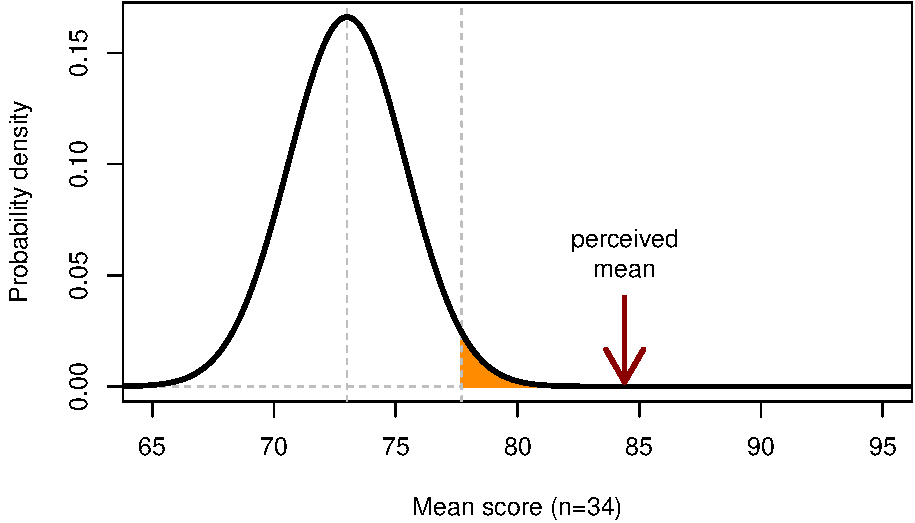
\includegraphics{QMS-EN_files/figure-latex/gramm2013onesample-1.pdf}
\caption{\label{fig:gramm2013onesample}Probability distribution of the mean score from a sample (n=34) with a population mean 73 and population s.d. 14. The coloured area covers 5\% of the total area under the curve; outcomes along the X-axis of this area thus have a probability of at most 5\% of occurring if H0 is true.}
\end{figure}

Figure \ref{fig:gramm2013onesample} shows the probability of the
sample mean (\(n=34\)) if H0 is true. We see that the value 73 can have
the highest probability, but also 72 or 74 are probable mean scores
according to H0. However, a mean of 84.4 is very improbable, the probability
\(P\) of this mean score (height of the curve) is almost null according to
H0.

The boundary value for \(P\), at which we reject H0 is called the significance
level, often referred to with the symbol \(\alpha\) (see
§\ref{sec:empiricalcycle}). Researchers often use \(\alpha=.05\),
but sometimes other boundary values are also used. In Figure
\ref{fig:gramm2013onesample}, you see that the probability of a mean score
of 77.7 or more has a probability of \(P=.05\) or smaller, according to
H0. This can be seen from the area under the curve. The coloured part has
precisely an area of 0.05 of the total area under
the curve.

The decision about whether or not to reject H0 is based on the probability
\(P\) of the outcomes, given H0. The decision might also be
incorrect. The finding that \(P < \alpha\) is thus not an
\emph{irrefutable} proof that H0 is untrue (and \emph{has to} be
rejected); it is also true that H0 is in fact true but that the
effect found was a fluke (Type 1 error). Conversely, the finding
that \(P > \alpha\) is not conclusive evidence that H0 is true. There can
be all kinds of other, plausible reasons why an effect which exists (H0 is untrue)
can still not be observed. If I do not hear any birds singing, that does not necessarily
mean that there are genuinely no birds singing. More generally: ``absence of evidence is not
evidence of absence'' (; ). It is thus good to always report the size
of the effect found (this is explained in more detail in
§@ref(\#sec:ttest-effectsize) below).

\begin{center}\rule{0.5\linewidth}{0.5pt}\end{center}

\begin{quote}
\emph{Example 13.1:}
Assume H0: `birds do not sing'. Write
down at least 4 reasons why I do not hear birds singing, even
if there are in fact birds singing (H0 is untrue). If I do not reject H0,
what type of error will I be making?
\end{quote}

\begin{center}\rule{0.5\linewidth}{0.5pt}\end{center}

\hypertarget{sec:ttest-onesample}{%
\section{\texorpdfstring{One-sample \(t\)-test}{One-sample t-test}}\label{sec:ttest-onesample}}

The Student's \(t\)-test is used to investigate a difference
between the mean score of a sample, and an a priori assumed value
of the mean. We use this test when the standard deviation
\(\sigma\) in the population is unknown, and thus has to be estimated from
the sample. The line of thought is as follows.

We determine the test statistic \(t\) on the basis of the mean and the
standard deviation in the sample, and of the assumed mean (according to H0).
If H0 is true, then the value \(t=0\) is the most\\
probable. The larger the difference between the observed sample mean and the
assumed sample mean, the more \(t\) increases. If the test statistic \(t\) is larger than
a certain boundary value \(t*\), and thus \(t>t*\), then the probability of this test statistic,
if H0 is true, is very small: \(P(t|\textrm{H0}) < \alpha\). The probability of finding this result
if H0 is true is then so small that we decide to reject H0
(see §\ref{sec:empiricalcycle}). We speak then of a \emph{significant} difference:
the deviation between the observed and the expected mean is probably not a
coincidence.

In the earlier example of the grammar test with Linguistics students
(§\ref{sec:testing-introduction}), we already became acquainted with
this form of \(t\)-test.
If \(\overline{x}=84.4, s=8.4, n=34\), then the test statistic
is \(t=7.9\) according to formula \eqref{eq:t-onesample} below.

The probability distribution of test statistic \(t\) under H0 is known;
you can find the boundary value \(t^*\) in
Appendix \ref{app:criticaltvalues}. Put otherwise, if the test statistic \(t\)
is larger than the boundary value \(t^*\) which is stated in the table then
\(P(t|\textrm{H0})<\alpha\). To be able to use the table in Appendix
\ref{app:criticaltvalues}, we still have to introduce a new term,
namely the number of degrees of freedom. That term is
explained in
§\ref{sec:ttest-freedomdegrees} below.

With the number of degrees of freedom, you can look in Appendix
\ref{app:criticaltvalues} to see which boundary value \(t^*\) is needed
to achieve a certain p-value for the established test statistic
\(t=7.9\). Let us see what the p-value is for the established
test statistic \(t=7.9\). We firstly look for the degrees of freedom (`d.f.') in the left column.
If the number of degrees of freedom does not occur in the table, then, to err
on the side of caution, we should round down, here to 30 d.f. This determines the row
which is applicable for us. In the third column, we find \(t^*=1.697\). Our
established test statistic \(t=7.9\) is larger than this \(t^*=1.697\), thus the p-value
is smaller than the \(p=.05\) from the third column. If we go further right on
the same line, we see that the stated \(t^*\) increases further.\\
Our established test statistic \(t\) is even larger than \(t^*=3.385\) in the last column.
The p-value is thus even smaller than \(p=.001\) from the title of that last
column. (The statistical analysis program usually also calculates the p-value.)
We report
the result as follows:

\begin{quote}
The mean score of Linguistics students (class of 2013) is
84.4 (\(s=8.4\)); this is significantly better than the assumed
population mean of 73 (\(t(33)=7.9, p<.001\)).
\end{quote}

\hypertarget{sec:ttest-freedomdegrees}{%
\subsection{Degrees of freedom}\label{sec:ttest-freedomdegrees}}

To explain the concept of degrees of freedom, we begin with an
analogy. Imagine that there are three possible routes for getting
from A to B: a coast path, a mountain path, and a motorway. It is true that a walker
who wants to travel from A to B has three options but there are only
two degrees of freedom for the walker: he or she only has to make
two choices to choose from the three options. Firstly, the motorway drops out
(first choice), and then the mountain path (second choice),
and then the chosen route along the coast is the only one left over. There are thus two
choices `free' in order to choose one of the three possible routes in the end.
If we know the two choices, then we can deduce from them which
route must have been chosen.

Now, we will look at a student who on average has achieved a \(\overline{x}=7.0\)
over the \(N=4\) courses from the first introductory track of his or her
degree programme. The mean of \(7.0\) can be arrived at in many ways,
e.g.~\((8,7,7,6)\) or \((5,6,8,9)\). But if we know the result of three of the courses,
and we also know that the mean is a 7.0 then we also know what the value
of the fourth observation must be. This last observation is thus no longer
`free' but is now fixed by the first three observations, in combination
with the mean over \(N=4\) observations. We then say that you have \(N-1\)
degrees of freedom to determine this characteristic of the sample, like the sample mean here, or like the test statistic \(t\).
The degrees of freedom is often abbreviated to `d.f.' (symbol \(\nu\), Greek letter ``nu'').

In practice, the number of degrees of freedom is not difficult to determine.
We namely indicate for every test how the degrees of freedom are established
--- and the number of d.f. is usually also calculated by the
statistical analysis program which we use.

For the \(t\)-test of a single sample, the number of degrees of freedom is the
number of observations \(N-1\). In the above discussed example, we thus have
\(N-1 = 34-1 = 33\) degrees of freedom.

\hypertarget{sec:formulas13-1}{%
\subsection{formulas}\label{sec:formulas13-1}}

\begin{equation}
  t = \frac{ \overline{y}-\mu} { s } \times \sqrt{N}
  \label{eq:t-onesample}
\end{equation}

\hypertarget{sec:ttest-assumptions}{%
\subsection{assumptions}\label{sec:ttest-assumptions}}

The \(t\)-test for a single sample requires three assumptions which
must be satisfied in order to be able to use the test.

\begin{itemize}
\item
  The data must have been measured on an interval level of measurement (see
  Chapter \ref{ch:levelsofmeasurement}).
\item
  All the observations have to be independent of each other.
\item
  The scores must be normally distributed (see
  §\ref{sec:normaldistribution}).
\end{itemize}

\hypertarget{spss-10}{%
\subsection{SPSS}\label{spss-10}}

The above discussed data can be found in the file \texttt{data/grammaticatoets2013.csv}.

To test our earlier hypothesis, in SPSS, we firstly have
to select the observations of the Linguistics students.

\begin{verbatim}
Data > Select cases...
\end{verbatim}

Choose \texttt{If\ condition\ is\ satisfied} and click on the button \texttt{If...} to indicate
the conditions for selection (inclusion).~\\
Select the variable \texttt{progr} (drag to the panel on the right-hand side), pick
button \texttt{=}, and then type \emph{\texttt{TW}} (the Dutch label for ``Linguistics''), so that the whole condition is
\texttt{progr\ =\ TW}.

Afterwards, we can test our earlier hypothesis as follows:

\begin{verbatim}
Analyze > Compare Means > One-Sample T Test...
\end{verbatim}

Select variable (drag to the Test variable(s) panel).\\
Indicate which value of \(\mu\) has to be tested: set it as
Test Value \texttt{73}. Confirm \texttt{OK}.

The output contains both descriptive statistics and the results
of a \emph{two-sample} \(t\)-test.

When transferring this output, take good note of the warning in
§\ref{sec:plargerthannull} below: SPSS reports as if \texttt{p=.000} but that is untrue.

\hypertarget{r-12}{%
\subsection{R}\label{r-12}}

Our hypothesis discussed above can be tested with the following exercises:

\begin{Shaded}
\begin{Highlighting}[]
\NormalTok{gramm2013 \textless{}{-}}\StringTok{ }\KeywordTok{read.csv}\NormalTok{( }\DataTypeTok{file=}\StringTok{"data/grammaticatoets2013.csv"}\NormalTok{,}\DataTypeTok{header=}\NormalTok{F)}
\KeywordTok{dimnames}\NormalTok{(gramm2013)[[}\DecValTok{2}\NormalTok{]] \textless{}{-}}\StringTok{ }\KeywordTok{c}\NormalTok{(}\StringTok{"score"}\NormalTok{,}\StringTok{"progr"}\NormalTok{)}
\CommentTok{\# program levels have Dutch labels: TW=Linguistics}
\KeywordTok{with}\NormalTok{( gramm2013,}
      \KeywordTok{t.test}\NormalTok{( score[progr}\OperatorTok{==}\StringTok{"TW"}\NormalTok{], }\DataTypeTok{mu=}\DecValTok{73}\NormalTok{, }\DataTypeTok{alt=}\StringTok{"greater"}\NormalTok{ ) )}
\end{Highlighting}
\end{Shaded}

\begin{verbatim}
## 
##  One Sample t-test
## 
## data:  score[progr == "TW"]
## t = 7.9288, df = 33, p-value = 1.913e-09
## alternative hypothesis: true mean is greater than 73
## 95 percent confidence interval:
##  81.97599      Inf
## sample estimates:
## mean of x 
##  84.41176
\end{verbatim}

The notation \texttt{1.913e-09} must be read as the number
\((1.913 \times 10^{-9})\).

\hypertarget{sec:plargerthannull}{%
\section{\texorpdfstring{\(p\)-value is always larger than zero}{p-value is always larger than zero}}\label{sec:plargerthannull}}

The p-value \(p\) can be very small but it is always larger than zero!
In the grammar test example above,
we found \(P=.000000001913\), a very small probability but one that is larger
than zero. This can also be seen from the tails of the corresponding
probability distribution which approach zero asymptotically (see
Fig.\ref{fig:gramm2013onesample}) but never become completely equal
to zero. There is always a minimally small probability of finding
an extreme value (or an even more extreme value) from you test statistic
in a sample --- after all, we are investigating the sample precisely
because the outcome of the test statistic cannot be established a priori.

In SPSS, however, the p-value is rounded off, and can then appear as
\texttt{‘Sig.\ .000’} or \(p=.000\). This is incorrect.
The p-value or significance is not equal to zero, but has
been \emph{rounded off} to zero, and that is not the same.
Always report the p-value or significance with the correct
accuracy, in this example as \(p<.001\) or even \(p<.0005\)
(taking into account the rounding off by SPSS to three decimal
places).

\hypertarget{sec:ttest-onesidedtwosided}{%
\section{One-sided and two-sided tests}\label{sec:ttest-onesidedtwosided}}

The procedure which we discussed above is valid for one-sided
tests. This is to say that the alternative hypothesis does not only put forward
that the means will differ but also in which direction that will be:
H1: \(\mu >73\), the Linguistics students score \emph{better} than the population
mean. If we were to find a difference in the opposite direction,
say \(\overline{x}=68\), then we would not even conceive of statistical testing:
the H0 simply still stands. It is only when we find a difference
in the hypothesised direction that it is meaningful to inspect whether
this difference is significant. When you look now at the figure in
Appendix \ref{app:criticaltvalues}, then this is also the case. The \(p\)-value
corresponds with the area of the coloured region.

If the alternative hypothesis H1 does \emph{not} specify the direction of the
difference, then a complication arises. Differences in any of the two possible directions
are relevant. We speak then of two-sided tests or two-tailed tests.\\
To calculate the two-sided p-value, we multiply the \(p\)-value from
Appendix \ref{app:criticaltvalues} by \(2\) (because we are now looking at two
coloured regions, on the lower and upper sides of the probability distribution).

In the grammar test example, let us now use a two-sided test. We
then operationalise the alternative hypothesis as H1: \(\mu \ne 73\).
Again, there is \(\overline{x}=73, t=7.9\) with 33 d.f. (rounded off to 30 d.f.).
With the one-sample p-value \(p=.025\) (fourth column), we find
the critical value \(t^*=2.042\). The two-sided p-value\\
for this critical value is \(2 \times .025 = .05\). The test statistic we found
\(t=7.9\) is larger than this \(t^*=2.042\), thus the two-sided
p-value is smaller than \(p=2\times.025=.05\). The test statistic we found
is larger even than \(t^*=3.385\) in the last column,
thus the two-sided p-value is even smaller than
\(2\times.001\). We can report our two-sided testing as
follows:

\begin{quote}
The mean score of Linguistics students (class of 2013) is
84.4 (\(s=8.4\)); the differs significantly from the hypothesised
population mean of 73 (\(t(33)=7.9, p<.002\)).
\end{quote}

In the majority of studies two-sided tests are used; if the direction
of the test is not stated then you may assume that two-sided or two-tailed tests
have been used.

\hypertarget{sec:t-confidenceinterval-mean}{%
\section{Confidence interval of the mean}\label{sec:t-confidenceinterval-mean}}

This section looks more deeply into a subject that was already discussed in
§\ref{sec:confidenceinterval-mean}, and illustrates the confidence interval
of the mean with the grammar test scores.

We can consider the sample's mean, \(\overline{x}\), as a good estimation
of an unknown mean in the population,
\(\mu\). For this, we can also use the value found for \(t^*\) to indicate how
reliable the estimation is: the confidence interval. With this, we express
with what (un)certainty we know that the sample mean, \(\overline{x}\), matches
the population mean \citep{Cumm12}. We are also familiar with such error margins
from election results, where they indicate with what certainty the result
of the sample (of respondents) matches the actual election result for the whole
population (of voters). An
error margin of 2\% means that it is 95\% certain that \(x\), the percentage voting
for a certain party, will lie between \((x-2)\)\% and \((x+2)\)\%.

In our example with 30 d.f., we find \(t^*=2.042\) for 95\%
reliability. Via formula
\eqref{eq:t-onesampleCI}, we arrive at the 95\%
confidence interval \((81.5, 87.3)\). We know with 95\% certainty
that the unknown average score on the grammar test, from the population
of all possible Linguistics students is larger than 81.5 and
smaller than 87.3. We thus also know, with 95\% certainty, that the
\emph{unknown} population mean \(\mu\) deviates from the hypothesised
value 73 \citep{Cumm12}. We report this as follows:

\begin{quote}
The mean score of Linguistics students (class of 2013) is
84.4, with 95\% confidence interval (81.5, 87.3), 33 d.f.
\end{quote}

In Figure \ref{fig:gramm2013CIs}, you can see the results of
a computer simulation to illustrate this. This figure is made in the same way as Figure
\ref{fig:tempo95CIs} in Chapter \ref{ch:probability-distributions} and
illustrates the same point. We have drawn \(100\times\) samples from Linguistics students,
with \(\mu=84.4\) and \(\sigma=8.4\) (see §\ref{sec:standarddeviation}) and \(N=34\).
For each sample, we have drawn the 95\%
confidence interval. For 95 of the 100 samples, the population mean \(\mu=84.4\)
is indeed within the interval, but for 5 of the 100 samples the confidence interval does not contain the population mean (these are marked along the right hand side).

\begin{figure}
\centering
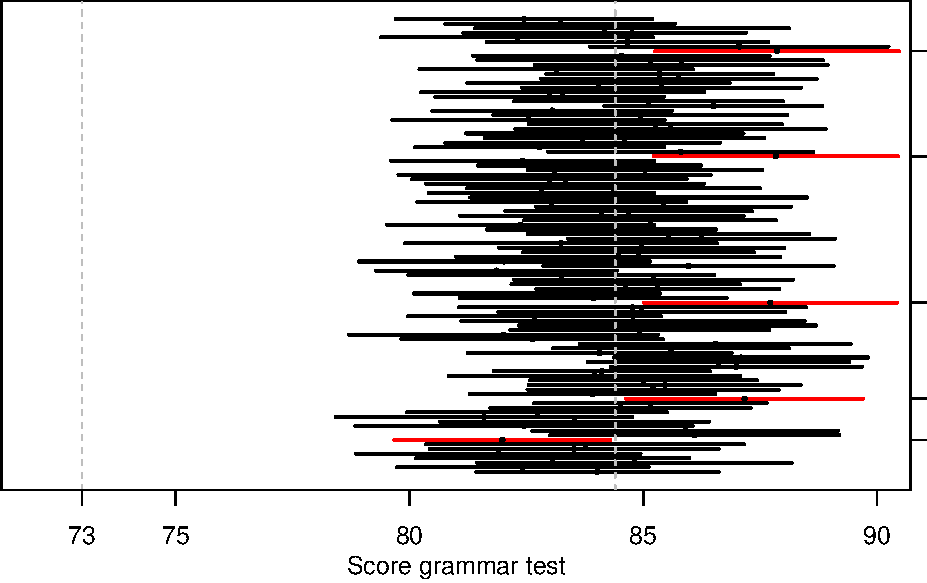
\includegraphics{QMS-EN_files/figure-latex/gramm2013CIs-1.pdf}
\caption{\label{fig:gramm2013CIs}95\% confidence interval and sample means, over 100 simulated samples (n=34) from a population with population mean 84.4, population-s.d. 8.4.}
\end{figure}

\hypertarget{sec:formulas13-2}{%
\subsection{formulas}\label{sec:formulas13-2}}

The two-sample confidence interval for \(B\)\% reliability for\\
a population mean \(\overline{y}\) is
\begin{equation}
    \overline{y} \pm t^*_{N-1} \times \frac{s}{\sqrt{N}}
  \label{eq:t-onesampleCI}
\end{equation}

\hypertarget{spss-11}{%
\subsection{SPSS}\label{spss-11}}

\begin{verbatim}
Analyze > Descriptive Statistics > Explore...
\end{verbatim}

Select dependent variables (drag to Dependent List panel).\\
Click on button \texttt{Statistics} and tick \texttt{Descriptives} with Confidence Interval
95\%.\\
Confirm with \texttt{Continue} and with \texttt{OK}.\\
The output contains several descriptive statistic measures, now also
including the 95\% confidence interval of the mean.

\hypertarget{r-13}{%
\subsection{R}\label{r-13}}

R states the confidence interval of the mean (with self-specifiable
confidence level) for a \(t\)-test. We thus again conduct a \(t\)-test
and find the confidence interval of the mean in the
output.

\begin{Shaded}
\begin{Highlighting}[]
\KeywordTok{with}\NormalTok{( gramm2013, }\KeywordTok{t.test}\NormalTok{( score[progr}\OperatorTok{==}\StringTok{"TW"}\NormalTok{] ) )}
\end{Highlighting}
\end{Shaded}

\begin{verbatim}
## 
##  One Sample t-test
## 
## data:  score[progr == "TW"]
## t = 58.649, df = 33, p-value < 2.2e-16
## alternative hypothesis: true mean is not equal to 0
## 95 percent confidence interval:
##  81.48354 87.33999
## sample estimates:
## mean of x 
##  84.41176
\end{verbatim}

\hypertarget{sec:ttest-indep}{%
\section{\texorpdfstring{Independent samples \(t\)-tests}{Independent samples t-tests}}\label{sec:ttest-indep}}

The Student's \(t\)-test is used to allow the investigation of a difference
between the mean scores of two independent samples, e.g of
comparable boys and girls. On the basis of the mean and the standard
deviations of the two samples, we determine the test statistic \(t\).
If H0 is true, then the value \(t=0\) is the most probable. The larger the difference
between the two means, the larger \(t\) is too. We again reject H0 if \(t>t^*\)
for the chosen significance level \(\alpha\).

As a first example, we will take a study of the productive vocabulary size
of 18-month old Swedish girls and boys \citep{Ande11}. We investigate the hypothesis
that the vocabulary of girls differs from that of boys, i.e.~
H1: \(\mu_m \ne \mu_j\).
We cannot a priori assume that a potential difference can only go in one direction;
we thus use a two-sided test, as already appears to be the case from H1.
The corresponding null hypothesis which we test is H0: \(\mu_m = \mu_j\).
In this study, the vocabulary is estimated on the basis of questionnaires
from the parents of the children in the sample. Participants were
(parents of) \(n_1=123\) girls and \(n_2=129\) boys, who were all 18 months
old. Based on the results, it seems that the girls have a mean vocabulary
of \(\overline{x_1}=95\) words (\(s_1=82\)), and for the boys it is
\(\overline{x_2}=85\) words (\(s_2=98\)). With these data, we determine the
test statistic \(t\) according to the formula
\eqref{eq:t-homoskedastic}, resulting in \(t=0.88\) with 122 d.f. We look for the
accompanying critical value \(t^*\) again in Appendix
\ref{app:criticaltvalues}. In the row for 100 d.f. (after rounding down),
we find \(t^*=1.984\) in the fourth column. For two-sample testing
we have to double the p-value which belongs to this column
(see §\ref{sec:ttest-onesidedtwosided}), resulting in \(p=.05\). The
test statistic \(t < t^*\), thus \(p>.05\). We decide \emph{not} to reject
H0, and report that as follows:

\begin{quote}
The mean productive vocabulary of Swedish 18-month old Swedish children
barely differs between girls and boys
(\(t(122)=0.88, p>.4\)). Girls produce on average 95 different
words (\(s=82\)), and boys on average 85 different words
(\(s=98\)).
\end{quote}

As a second example, we take a study of the speech tempo of two groups
of speakers, namely originating from the West (first group) and
from the North (second group) of the Netherlands. The speech tempo
is expressed here as the mean duration of a spoken syllable, in seconds,
over an interview of ca. 15 minutes (see Example \ref{ch:anova}.1).
We investigate H0: \(\mu_W = \mu_N\) with
two-sample testing. From the results, it appears that those from the West
(\(n=20\)) have a mean syllable duration of
\(\overline{x_W}=0.235\) s (\(s=0.028\)), and that for those from the North (also
\(n=20\)) that is \(\overline{x_N}=0.269\) s (\(s=0.029\)). With these data,
we again determine the test statistic \(t\) according to the formula
\eqref{eq:t-homoskedastic}, resulting in \(t=-3.76\) with 38 d.f. We look for
the accompanying critical value again in Appendix
\ref{app:criticaltvalues}. The correct d.f. are not stated in the table
so we round them down (i.e.~in the conservative direction) to
30 d.f. In the row, we find \(t^*=2.042\) in the fourth column.
For two-sample testing, we have to double the p-value corresponding to
these columns (see
§\ref{sec:ttest-onesidedtwosided}), resulting in \(p=.05\). The
test statistic is \(t < t^*\), thus \(p<.05\). We thus decide
to \emph{indeed} reject H0, and report that as follows:

\begin{quote}
The mean duration of a syllable spoken by a speaker from the West
of the Netherlands is \(0.235\) seconds (\(s=0.028\)). This is
significantly shorter than from speakers from the North of the Netherlands
(\(\overline{x}=0.269\) s, \(s=0.029\)) (\(t(38)=-3.76, p<.05\)). In the
investigated recordings from 1999, the speakers from the West thus
speak more quickly than those from the North of the Netherlands.
\end{quote}

\hypertarget{assumptions}{%
\subsection{assumptions}\label{assumptions}}

The Student's \(t\)-test for two independent samples requires four assumptions
which must be satisfied in order to use the test.

\begin{itemize}
\item
  The data has to be measured on an interval level of measurement (see
  §\ref{sec:interval}).
\item
  All the observations must be independent of each other.
\item
  Both groups' scores must be normally distributed (see
  §\ref{sec:isvarnormaldistributed}).
\end{itemize}

The variance of the scores has to be equal in both
samples. The more the two samples differ in size, the more
serious the violation of this assumption is. It is thus prudent
to work with equally large, and preferably not too small samples. If the
samples are equally large, then the violation of this assumption of equal
variances is not so serious.

\hypertarget{sec:ttest-formulas}{%
\subsection{formulas}\label{sec:ttest-formulas}}

\hypertarget{test-statistic}{%
\subsubsection{test statistic}\label{test-statistic}}

To calculate test statistic \(t\), various formulas are used.

If the samples have about equal variance, then we firstly use
the ``pooled standard deviation'' \(s_p\) as an intermediate step. In this, both
standard deviations from the two samples are weighted according
to their sample size.
\begin{equation}
    s_p = \sqrt{ \frac{(n_1-1) s^2_1 + (n_2-1) s^2_2} {n_1+n_2-2} }
    \label{eq:sd-pooled}
\end{equation}
Then
\begin{equation}
  \label{eq:t-homoskedastic}
  t = \frac{ \overline{x_1}-\overline{x_2} } { s_p \sqrt{\frac{1}{n_1}+\frac{1}{n_2}} }
\end{equation}

If the samples do \emph{not} have equal variance, and the fourth assumed
sample above is thus violated, then Welch's t-test is
used:
\begin{equation}
  \label{eq:sd-WS}
  s_{\textrm{WS}} = \sqrt{\frac{s^2_1}{n_1}+\frac{s^2_2}{n_2} }
\end{equation}
Then
\begin{equation}
  \label{eq:t-WS}
  t = \frac{ \overline{x_1}-\overline{x_2} } { s_{\textrm{WS}} }
\end{equation}

\hypertarget{freedomdegrees}{%
\subsubsection{degrees of freedom}\label{freedomdegrees}}

The t-test is usually conducted by a computer program. There,
the following approximation of degrees of freedom is usually used
(\(\nu\), see §\ref{sec:ttest-freedomdegrees}).
Firstly, \(g_1=s^2_1/n_1\)
and \(g_2=s^2_2/n_2\) are calculated. The number of degrees of freedom of \(t\) is then
\begin{equation}
  \label{eq:df-WS}
  \nu_\textrm{WS} = 
        \frac {(g_1+g_2)^2} {g^2_1/(n_1-1) + g^2_2/(n_2-1)}
\end{equation}

According to this approximation, the number of degrees of freedom has as its liberal
upper limit \((n_1+n_2-2)\), and as its conservative lower limit the smallest
of \((n_1-1)\) or \((n_2-1)\). You can thus always use this conservative
lower limit. If the two groups have around the same variance
(i.e.~\(s_1 \approx s_2\)), then you can also use the liberal lower
limit.

For the second example above, the approximation of formula
\eqref{eq:df-WS} gives
an estimation of \(37.99 \approx 38\) d.f. The conservative lower limit is
\(n_1-1 = n_2-1 = 19\). The liberal lower limit is \(n_1+n_2 -2 = 38\). (In
the table with critical values \(t*\), in
Appendix \ref{app:criticaltvalues}, it is usually advisable to use the row
with the first-following smaller value for the number of
degrees of freedom.)

\hypertarget{sec:SPSS-ttest-unpaired}{%
\subsection{SPSS}\label{sec:SPSS-ttest-unpaired}}

Here, the second example above is worked out.

\begin{verbatim}
Analyze > Compare Means > Independent-Samples T Test
\end{verbatim}

Drag the dependent variable \texttt{syldur} to the Test Variable(s) panel.
Drag the independent variable \texttt{region} to the Grouping
Variable panel. Define the two groups: value \texttt{W} for region group 1 and\\
value \texttt{N} for region group 2. Confirm with \texttt{Continue} and \texttt{OK}.

As you could see above the calculation of the \(t\)-test is dependent on the
answer to the question whether the standard deviations of the two groups
are around equal. SPSS solves this rather clumsily: you get to see all the
relevant outputs, and have to make a choice from them yourself.

\hypertarget{test-for-equality-of-variances}{%
\subsubsection{Test for equality of variances}\label{test-for-equality-of-variances}}

With Levene's test, you can investigate H0: \(s^2_1 = s^2_2\), i.e.~whether
the variances (and with them the standard deviations) of the two groups
are equal. If you find a small value for the test statistic \(F\),
and a \(p>.05\), then you do not have to reject this H0. You can then assume
that the variances are equal. If you find a large value for \(F\),
with \(p<.05\), then you should indeed reject this H0, and you cannot
assume that the variances of these two groups are equal.

\hypertarget{test-for-equality-of-means}{%
\subsubsection{Test for equality of means}\label{test-for-equality-of-means}}

Depending on this outcome from Levene's test, you have to use the first
or the second row of the output of the Independent Samples Test
(a test which investigates whether the means from the two groups are equal).
In this example, the variances are around equal, as the
Levene's test also indicates. We thus use the first line of the output,
and report \(t(38)=-3.765, p=.001\).

\hypertarget{sec:R-ttest-unpaired}{%
\subsection{R}\label{sec:R-ttest-unpaired}}

\begin{Shaded}
\begin{Highlighting}[]
\KeywordTok{require}\NormalTok{(hqmisc)}
\KeywordTok{data}\NormalTok{(talkers)}
\KeywordTok{with}\NormalTok{(talkers, }\KeywordTok{t.test}\NormalTok{( syldur[region}\OperatorTok{==}\StringTok{"W"}\NormalTok{], syldur[region}\OperatorTok{==}\StringTok{"N"}\NormalTok{], }
            \DataTypeTok{paired=}\NormalTok{F, }\DataTypeTok{var.equal=}\NormalTok{T ) )}
\end{Highlighting}
\end{Shaded}

\begin{verbatim}
## 
##  Two Sample t-test
## 
## data:  syldur[region == "W"] and syldur[region == "N"]
## t = -3.7649, df = 38, p-value = 0.0005634
## alternative hypothesis: true difference in means is not equal to 0
## 95 percent confidence interval:
##  -0.0519895 -0.0156305
## sample estimates:
## mean of x mean of y 
##   0.23490   0.26871
\end{verbatim}

\hypertarget{sec:ttest-paired}{%
\section{\texorpdfstring{\(t\)-test for paired observations}{t-test for paired observations}}\label{sec:ttest-paired}}

The Student's \(t\)-test is also used to investigate a difference between the
means of two dependent or paired observations. This is the case if we only draw
one sample (see Chapter
\ref{ch:samples}), and then collect two observations from the members of this
sample,
namely one observation under each of the conditions. The two
observations are then paired, i.e.~related to each other,
and these observations are thus not independent (since they come
from the same member of the sample). With this, one of the assumptions of
the \(t\)-test is violated.

As an example, we take an imaginary investigation of the use of the
Dutch second person pronouns \emph{U} (formal ``you'', like French ``vous'') and \emph{je} (informal ``you'', like French ``tu'') as forms of address on a website. The researcher makes two versions
of a website, one with \emph{U} and the other with \emph{je}. Each
respondent has to judge both versions on a scale from 1 to 10. (For validity
reasons, the order of the two versions is varied between respondents;
the order in which the pages are judged can thus
have no influence on the total score per condition.) In Table
\ref{tab:data-uje-paired}, the judgements of \(N=10\)
respondents are summarised.

\begin{longtable}[]{@{}cllc@{}}
\caption{\label{tab:data-uje-paired} Fictional judgements of a webpage
with \emph{U} or \emph{je} as the forms of addressed, by \(N=10\) respondents.}\tabularnewline
\toprule
ID & \emph{U} Condition & \emph{je} Condition & \(D\)\tabularnewline
\midrule
\endfirsthead
\toprule
ID & \emph{U} Condition & \emph{je} Condition & \(D\)\tabularnewline
\midrule
\endhead
1 & 8 & 9 & -1\tabularnewline
2 & 5 & 6 & -1\tabularnewline
3 & 6 & 9 & -3\tabularnewline
4 & 6 & 8 & -2\tabularnewline
5 & 5 & 8 & -3\tabularnewline
6 & 4 & 6 & -2\tabularnewline
7 & 4 & 8 & -4\tabularnewline
8 & 7 & 10 & -3\tabularnewline
9 & 7 & 9 & -2\tabularnewline
10 & 6 & 7 & -1\tabularnewline
& & & \(\overline{D}\)=-2.2\tabularnewline
\bottomrule
\end{longtable}

The pair of observations for the \(i\)-th member of the sample has a
difference score which we can write as:\\
\(D_i = x_{1i} - x_{2i}\) where \(x_{1i}\) is the dependent
variable score of the \(i\)-th respondent for condition 1. This
difference score is also stated in
Table~\ref{tab:data-uje-paired}.

This difference score \(D\) is then actually analysed with the earlier discussed \(t\)-test for a single sample (see
§\ref{sec:ttest-onesample}), where H0: \(\mu_D=0\), i.e.~according to H0, there is no
difference between conditions. We calculate the mean of the difference score,
\(\overline{D}\), and the standard variance of the difference score, \(s_{D}\),
in the usual manner (see
§\ref{sec:standarddeviation}). We use this mean and this
standard deviation to calculate the test statistic \(t\) via formula
\eqref{eq:t-pairedsamples}, with \((N-1)\) degrees of freedom. Finally,
we again use
Appendix \ref{app:criticaltvalues} to determine the critical value.
and with it, the p-value \(p\) for the value of the sample size
\(t\) under H0.

For the above example with \emph{U} or \emph{je} as forms of address,
we thus find \(\overline{D}=-2.2\) and \(s_D=1.0\). If we put this into
formula \eqref{eq:t-pairedsamples}, we find \(t=-6.74\) with \(N-1=9\) d.f.
We again look for the corresponding critical value \(t^*\)
in Appendix \ref{app:criticaltvalues}. Thereby, we ignore the sign of \(t\),
because, after all, the probability distribution of \(t\) is symmetric.
In the row for 9 d.f., we find \(t^*=4.297\) in the last column.
For two-sided testing, we have to double the p-value corresponding to this
column (see
§\ref{sec:ttest-onesidedtwosided}), resulting in \(p=.002\).
The test statistic is \(t > t^*\), thus \(p<.002\). We decide to
\emph{indeed} reject H0, and report that as follows:

\begin{quote}
The judgement of \(N=10\) respondents on the page with \emph{U} as the
form of address is on average 2.2 points lower than their judgement
over the comparable page with \emph{je} as the form of address; this is
a significant difference (\(t(9)=-6.74, p<.002\)).
\end{quote}

\hypertarget{assumptions-1}{%
\subsection{assumptions}\label{assumptions-1}}

The \(t\)-test for paired observations within a single sample requires three
assumptions which must be satisfied, in order to be able to use these
tests.

\begin{itemize}
\item
  The data must be measured on an interval level of measurement (see
  §\ref{sec:interval}).
\item
  All \emph{pairs} of observations have to be independent of
  each other.
\item
  The \emph{difference scores} \(D\) have to be normally distributed (see\\
  §\ref{sec:isvarnormaldistributed}); however, if the number of pairs of
  observations in the sample is larger than ca. 30 then the t-test is
  usually useable.
\end{itemize}

\hypertarget{sec:formulas13-4}{%
\subsection{formulas}\label{sec:formulas13-4}}

\begin{equation}
  \label{eq:t-pairedsamples}
  t = \frac{ \overline{D}-\mu_D} { s_D } \times \sqrt{N}
\end{equation}

\hypertarget{sec:SPSS-ttest-paired}{%
\subsection{SPSS}\label{sec:SPSS-ttest-paired}}

The data for the above example can be found in the file \texttt{data/ujedata.csv}.

\begin{verbatim}
Analyze > Compare Means > Paired-Samples T Test
\end{verbatim}

Drag the first dependent variable \texttt{cond.u} to the Paired
Variables panel under Variable1, and drag the second variable \texttt{cond.je} to
the same panel under Variable2. Confirm with \texttt{OK}.

\hypertarget{sec:R-ttest-paired}{%
\subsection{}\label{sec:R-ttest-paired}}

The data from the above example can be found in the file \texttt{data/ujedata.csv}.

\begin{Shaded}
\begin{Highlighting}[]
\NormalTok{ujedata \textless{}{-}}\StringTok{ }\KeywordTok{read.table}\NormalTok{( }\DataTypeTok{file=}\StringTok{"data/ujedata.csv"}\NormalTok{, }\DataTypeTok{header=}\OtherTok{TRUE}\NormalTok{, }\DataTypeTok{sep=}\StringTok{";"}\NormalTok{ )}
\KeywordTok{with}\NormalTok{(ujedata, }\KeywordTok{t.test}\NormalTok{( cond.u, cond.je, }\DataTypeTok{paired=}\OtherTok{TRUE}\NormalTok{ ) )}
\end{Highlighting}
\end{Shaded}

\begin{verbatim}
## 
##  Paired t-test
## 
## data:  cond.u and cond.je
## t = -6.7361, df = 9, p-value = 0.00008498
## alternative hypothesis: true difference in means is not equal to 0
## 95 percent confidence interval:
##  -2.938817 -1.461183
## sample estimates:
## mean of the differences 
##                    -2.2
\end{verbatim}

\hypertarget{sec:ttest-effectsize}{%
\section{Effect size}\label{sec:ttest-effectsize}}

Until now, we have mainly dealt with testing as a binary
decision with regards to whether or not to reject H0, in the light
of the observations. However, in addition to this, it is also of great importance
to know how large the observed effect actually is: the \emph{effect size} (`ES')
\citep{Cohen88, Thom02, Naka07}.

In the formulas \eqref{eq:t-onesample} and \eqref{eq:t-pairedsamples}, it is expressed that the larger the effect gets, the larger \(t\) gets,
i.e.~for a larger difference
\((\overline{x}-\mu)\) or \((\overline{x_1}-\overline{x_2})\) or
\((\overline{D}-\mu_D)\){]}, \emph{and.or} the larger the sample gets.
Put briefly \citep[ p.338, formula 11.10]{Rose08}:
\begin{equation}
  \label{eq:Rose08}
    \textrm{significance test} = 
    \textrm{size of effect} \times \textrm{size of study}
\end{equation}

This means
that a small, and possibly trivial effect can also be
statistically significant if only the sample is large enough.
Conversely, a very large effect can be firmly established on the basis of
a very small sample.

\begin{center}\rule{0.5\linewidth}{0.5pt}\end{center}

\begin{quote}
\emph{Example 13.2:}
In an investigation of the life times of inhabitants from Austria
and Denmark \citep{Dobl99}, it appears that life times differ according to
the week of birth. This is presumably because babies from ``summer pregnancies''
are (or were) on average somewhat healthier than those
from ``winter pregnancies''. In this investigation, the differences
in life times were very small \(\pm 0.30\) year in Austria, \(\pm 0.15\) year
in Denmark), but the number of observations (deceased persons) was very large.
\end{quote}

\begin{quote}
Meanwhile, the difference in body length between dwarfs (shorter than
1.5 m) and giants (taller than 2.0 m) is so large that the difference can be firmly
empirically established on the basis of only \(n=2\) in each group.
\end{quote}

\begin{center}\rule{0.5\linewidth}{0.5pt}\end{center}

In our investigation, we are especially interested in important
differences, i.e.~usually large differences. We have to appreciate
that studies also entail costs in terms of money, time,
effort, privacy, and loss of naïveté for other studies
(see Chapter
\ref{ch:integrity}). We thus do not what to want to perform studies
on trivial effects needlessly. A researcher should thus determine in advance
what the smallest effect is that he/she wants to be able to detect, e.g.
1 point difference in the score of the grammar test. Differences smaller than
1 point are then considered to be trivial, and differences larger than 1 point to be potentially
interesting.

It is also important to state the effect size found with the results
of the study, to be of service for readers and later
researchers. In some academic journals, it is even
required to report the effect size. It should be said that this
can also be in the form of a confidence interval of the mean
(see~\ref{sec:t-confidenceinterval-mean}), because we can
convert these confidence intervals and effect sizes into
each other.

The raw effect size is straightforwardly the difference \(D\) in means
between the two groups, or between two conditions, expressed in units
of the raw score. In §\ref{sec:ttest-indep}, we found such a difference
in vocabulary of \(D=95-85=10\) between boys and girls.

However, we mainly use the standardised effect size (see
the formulas below), where we take into account the distribution in
the observations, e.g.~in the form of ``pooled standard deviation'' \(s_p\) \footnote{In this case, we use \(s_p = \sqrt{ \frac{122\times82^2+128\times98^2} {122+128} } = 90.5\), see formulas
  \eqref{eq:sd-pooled} and \eqref{eq:d-homoskedastic}.}.
In this way, we find a standardised effect size of
\begin{equation}
  \label{eq:d-standardized}
    d = \frac{ \overline{x_1}-\overline{x_2} } {s_p} = \frac{10}{90.5} = 0.11
\end{equation}
In the first example below, the standardised effect size of the difference in
vocabulary between girls and boys is thus 0.11. In this case, the difference
between the groups is small with respect to the distribution
within the groups --- the probability that a randomly selected girl
has a larger vocabulary than a randomly selected boy, is only 0.53 \citep{McGraw92},
and that is barely better than the probability of 0.50 which we expect according to H0.
It is then no surprise that this very small effect is not significant
(see §\ref{sec:ttest-indep}). We could
report the effect size and significance as follows:

\begin{quote}
The mean productive vocabulary of Swedish 18-month old children
barely differs between girls and boys. Girls
produce on average 95 different words (\(s=82\)), and boys
on average 85 different words (\(s=98\)). The difference is very
small (\(d=0.11)\) and not significant (\(t(122)=0.88, p>.4\)).
\end{quote}

In the second example above, the standardised effect size of the difference
in syllable length is about
\((0.235-0.269)/0.029 \approx 1.15\). We can report this relatively large
effect as follows:

\begin{quote}
The average length of a syllable spoken by a speaker from
the West of the Netherlands is \(0.235\) seconds (\(s=0.028\)). This is
considerably shorter than for speakers from the North of the Netherlands
(\(\overline{x}=0.269\) s, \(s=0.029\)). The difference is ca. 10\%; this
difference is very large (\(d=-1.15\)) and significant
(\(t(38)=-3.76, p<.05\)). In the investigated recordings from 1999, the
speakers from the West thus speak considerably more quickly than those from
the North of the Netherlands.
\end{quote}

If \(d\) is around 0.2, we speak of a small effect. We call an effect size
\(d\) of around 0.5 a medium effect, and we call one
of around 0.8 or larger a large effect \citep{Cohen88, Rose08}.

\begin{figure}
\centering
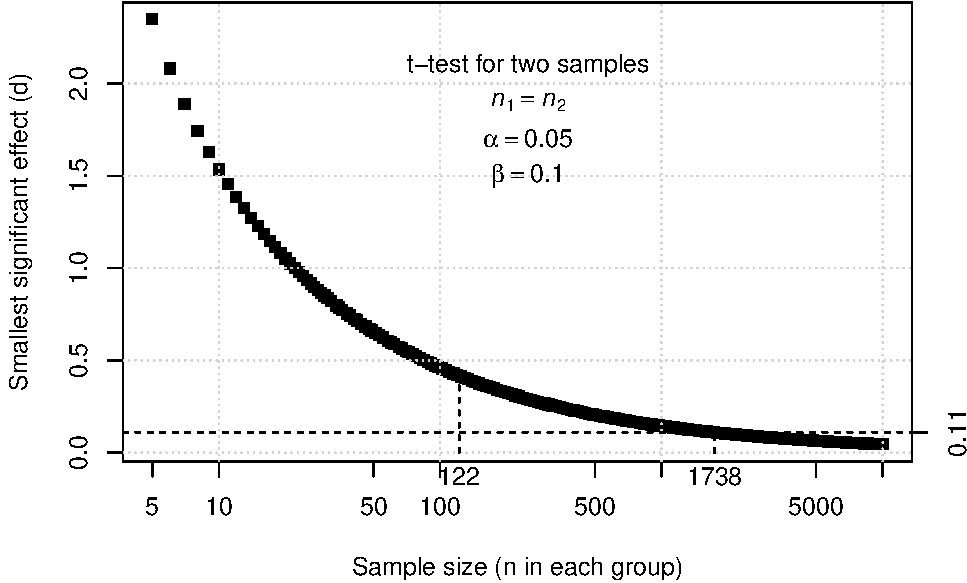
\includegraphics{QMS-EN_files/figure-latex/smallestsignifdifference-1.pdf}
\caption{\label{fig:smallestsignifdifference}Relation between the sample size and the smallest effect (d) that is significant according to a \emph{t}-test for unpaired, independent observations, with errors probabilities alpha=.05 and beta=.10.}
\end{figure}

\begin{center}\rule{0.5\linewidth}{0.5pt}\end{center}

\begin{quote}
\emph{Example 13.3:}
Look again at the formula \eqref{eq:Rose08}
and at the Figure \ref{fig:smallestsignifdifference} which illustrate
the relation between sample size and effect size. With an
effect size of \(n_1=122\), we can only detect an effect of \(d=0.42\)
or more, with sufficiently low probabilities of Type I and II errors again
(\(\alpha=.05\), \(\beta=.10\)). To detect the very small effect of \(d=0.11\),
with the same small error probabilities \(\alpha\) and \(\beta\), samples
of at least 1738 girls and 1738 boys would be needed.
\end{quote}

\begin{center}\rule{0.5\linewidth}{0.5pt}\end{center}

We can also express the effect size as the probability that
the difference occurs in the predicted direction, for a randomly
chosen element from the population
(formulas~\eqref{eq:d-onesample} and \eqref{eq:d-paired}),
or (if applicable) for two
randomly and independently chosen elements from the two populations
(formula~\eqref{eq:d-homoskedastic}) \citep{McGraw92}. Let us again return to
the grammar test from the Linguistics students
(§\ref{sec:ttest-onesample}). The effect which we found is
not only significant but also large. Expressed in terms of probability:
the probability that a random Linguistics student achieves a score
larger than \(\mu_0=73\) is 0.91. (And a randomly chosen
Linguistics student thus still has 9\% probability of achieving a lower score than
the hypothesised population mean of 73.)

For the fictional judgements about the webpages with \emph{U} or \emph{je} (see
Table~\ref{tab:data-uje-paired}), we find a standardised
effect size of
\[d = \frac{ \overline{D}-\mu_D} {s_D} = \frac{ -2.20-0 } {1.03} = -2.13\]
It is then not surprising that this extremely large effect is indeed
significant. We can report this as follows:

\begin{quote}
The judgements of \(N=10\) respondents about the pages with \emph{U} or \emph{je}
as forms of address differ significantly, with on average \(-2.2\) points
difference. This difference has a 95\% confidence interval of
\(-2.9\) to \(-1.5\) and an estimated standardised effect size
\(d=-2.13\); the probability that a randomly chosen respondent
judges the \emph{je}-version more highly than the \emph{U}-version is \(p=.98\).
\end{quote}

\hypertarget{sec:formulas13-5}{%
\subsection{formulas}\label{sec:formulas13-5}}

For a single sample:
\begin{equation}
   \label{eq:d-onesample}
  d = \frac{\overline{x}-\mu}{s}
\end{equation}
where \(s\) stands for the standard variation \(s\)
of the score \(x\).

For two independent samples (see
formula~\eqref{eq:sd-pooled}):
\begin{equation}
  \label{eq:d-homoskedastic}
  d = \frac{ \overline{x_1}-\overline{x_2} } { s_p }
\end{equation}

For paired observations:
\begin{equation}
  \label{eq:d-paired}
  d = \frac{ \overline{x_1}-\overline{x_2} } { s_D }
\end{equation}
where \(s_D\) is the
standard deviation from the difference \(D\) according
to the formula \eqref{eq:d-paired}.

\hypertarget{spss-13-2}{%
\subsection{SPSS}\label{spss-13-2}}

In SPSS, it is usually easiest to calculate the effect size
by hand.

For a simple sample
(formula~\eqref{eq:d-onesample}), we can simply calculate the
effect size from the mean and the standard deviation, taking into account
the value \(\mu\) which we are testing against.

\begin{verbatim}
Analyze > Descriptive Statistics > Descriptives...
\end{verbatim}

Choose the button \texttt{Options} and ensure that \texttt{Mean} and \texttt{Std.deviation} are
ticked. As a result there is the required data in the output:\\
\(d = (84.41 - 73) / 8.392 = 1.36\), a very large effect.

For unpaired, independent observations, it is likewise the easiest
to calculate the effect size by hand on the basis of the
means, standard deviations, and size of the two samples, making use
of the formulas
\eqref{eq:sd-pooled} and
\eqref{eq:d-homoskedastic} above.

For a single sample with two paired observations
(formula~\eqref{eq:d-paired}), we can again calculate the effect
size more simply from the mean and the standard deviation of the difference.
The data are in the output of the pairwise \(t\)-test\\
(§\ref{sec:SPSS-ttest-paired}), respectively as \texttt{Mean} and
\texttt{Std.Deviation}:\\
\(d = -2.200 / 1.033 = 2.130\), a super large effect.

\hypertarget{r-14}{%
\subsection{R}\label{r-14}}

In R, it is easier to have the effect size calculated.

For a single sample
(formula~\eqref{eq:d-onesample}):\\

\begin{Shaded}
\begin{Highlighting}[]
\NormalTok{gramm2013 \textless{}{-}}\StringTok{ }\KeywordTok{read.csv}\NormalTok{( }\DataTypeTok{file=}\StringTok{"data/grammaticatoets2013.csv"}\NormalTok{,}\DataTypeTok{header=}\NormalTok{F)}
\KeywordTok{dimnames}\NormalTok{(gramm2013)[[}\DecValTok{2}\NormalTok{]] \textless{}{-}}\StringTok{ }\KeywordTok{c}\NormalTok{(}\StringTok{"score"}\NormalTok{,}\StringTok{"progr"}\NormalTok{)}
\CommentTok{\# programs have Dutch labels, TW=Linguistics}
\KeywordTok{with}\NormalTok{(gramm2013, score[progr}\OperatorTok{==}\StringTok{"TW"}\NormalTok{]) {-}\textgreater{}}\StringTok{ }\NormalTok{score.ling}
\CommentTok{\# auxiliary variable}
\NormalTok{( }\KeywordTok{mean}\NormalTok{(score.ling)}\OperatorTok{{-}}\DecValTok{73}\NormalTok{ ) }\OperatorTok{/}\StringTok{ }\KeywordTok{sd}\NormalTok{(score.ling) }
\end{Highlighting}
\end{Shaded}

\begin{verbatim}
## [1] 1.359783
\end{verbatim}

The probability of a score larger than the population mean (the test value) \texttt{73} for a random Linguistics
student (of which we assume that \(\mu=84.4\) and \(s=8.4\)):

\begin{Shaded}
\begin{Highlighting}[]
\DecValTok{1} \OperatorTok{{-}}\StringTok{ }\KeywordTok{pnorm}\NormalTok{( }\DecValTok{73}\NormalTok{, }\DataTypeTok{mean=}\FloatTok{84.4}\NormalTok{, }\DataTypeTok{sd=}\FloatTok{8.4}\NormalTok{ ) }
\end{Highlighting}
\end{Shaded}

\begin{verbatim}
## [1] 0.9126321
\end{verbatim}

For unpaired, independent observations, we can calculate the smallest
significant effect (see also
Fig.~\ref{fig:smallestsignifdifference}); for which we use the function
\texttt{power.t.test}. (This function is
also used to construct Fig.\ref{fig:smallestsignifdifference}.)
With this function, you have to set the desired \texttt{power} as
an argument (power = \(1-\beta\); see
§\ref{sec:power-introduction}).

\begin{Shaded}
\begin{Highlighting}[]
\KeywordTok{power.t.test}\NormalTok{( }\DataTypeTok{n=}\DecValTok{122}\NormalTok{, }\DataTypeTok{sig=}\NormalTok{.}\DecValTok{05}\NormalTok{, }\DataTypeTok{power=}\NormalTok{.}\DecValTok{90}\NormalTok{, }\DataTypeTok{type=}\StringTok{"two.sample"}\NormalTok{ )}
\end{Highlighting}
\end{Shaded}

\begin{verbatim}
## 
##      Two-sample t test power calculation 
## 
##               n = 122
##           delta = 0.4166921
##              sd = 1
##       sig.level = 0.05
##           power = 0.9
##     alternative = two.sided
## 
## NOTE: n is number in *each* group
\end{verbatim}

In the output, the smallest significant effect is indicated by \texttt{delta}; see also
Example 13.3 above.

For a single sample with two paired observations
(formula\eqref{eq:d-paired}):

\begin{Shaded}
\begin{Highlighting}[]
\NormalTok{ujedata \textless{}{-}}\StringTok{ }\KeywordTok{read.table}\NormalTok{( }\DataTypeTok{file=}\StringTok{"data/ujedata.csv"}\NormalTok{, }\DataTypeTok{header=}\OtherTok{TRUE}\NormalTok{, }\DataTypeTok{sep=}\StringTok{";"}\NormalTok{ )}
\KeywordTok{with}\NormalTok{( ujedata, }\KeywordTok{mean}\NormalTok{(cond.u}\OperatorTok{{-}}\NormalTok{cond.je) }\OperatorTok{/}\StringTok{ }\KeywordTok{sd}\NormalTok{(cond.u}\OperatorTok{{-}}\NormalTok{cond.je) )}
\end{Highlighting}
\end{Shaded}

\begin{verbatim}
## [1] -2.130141
\end{verbatim}

\hypertarget{confidence-interval-of-the-effect-size}{%
\subsection{Confidence interval of the effect size}\label{confidence-interval-of-the-effect-size}}

Earlier, we already saw
(§\ref{sec:confidenceinterval-mean} and
§\ref{sec:t-confidenceinterval-mean})
that we can estimate a characteristic
or parameter of the population on the basis of a characteristic
from a sample. This is how we estimated the unknown population mean \(\mu\)
on the basis of the observed sample mean
\(\overline{x}\). The estimation does have a certain degree of
uncertainty or reliability: perhaps the unknown parameter differs
in the population somewhat from the sample characteristic,
which we use as an estimator, as a result of chance variations in the
sample. The (un)certainty and (un)reliability is expressed as
a confidence interval of the estimated characteristic. We then know
with a certain reliability (mainly 95\%) that the unknown parameter
will lie within that interval
(§\ref{sec:confidenceinterval-mean} and §\ref{sec:t-confidenceinterval-mean}).

This reasoning is now valid not only for the mean score, or for the mean or for the
variance, but equally for the effect size. After all, the effect size
is also an unknown parameter from the population, which we are trying to estimate
based on a limited sample. For the fictional judgements
about the webpages with the formal \emph{U} or informal \emph{je} pronouns (see
Table~\ref{tab:data-uje-paired}), we found a standardised effect size
of \(d=-2.13\). This is an estimation of the unknown
effect size (i.e.~of the strength of the preference for the \emph{je}-variant)
in the population of assessors, on the basis of a sample of \(n=10\)
assessors. We can also indicate the reliability of this estimation
here, in the form of a \emph{confidence interval} around the
observed sample \(d=-2.13\).

The confidence interval of the effect size is tricky to establish though
\citep{Naka07, Chen15}. We illustrate it here in a simple manner for
the simplest case, namely that of the \(t\)-test for a single sample,
or for two paired observations. For this, we need two elements:
firstly, the effect size expressed as a correlation \citep[ p.359, formula 12.1]{Rose08}, \[r = \sqrt{ \frac{t^2}{t^2+\textrm{df}} }\] and secondly
the standard error of the effect size \(d\) \citep[ p.600,
formula 18]{Naka07}:\\
\begin{equation}
  \label{eq:d-paired-se}
    \textrm{se}_d = \sqrt{ \frac{2(1-r)}{n} + \frac{d^2}{2(n-1)} }
\end{equation}

In
our earlier example of the \(n=10\) paired judgements about a webpage
with \emph{U} or \emph{je} as forms of address we found \(d=-2.13\). We also find
that \(r=.9135\). With these data, we find \(\textrm{se}_d = 0.519\) via
formula~\eqref{eq:d-paired-se}.

With this, we then determine the confidence interval for the
effect size:
\begin{equation}
   \label{eq:d-paired-CI}
    d \pm t^*_{n-1} \times \textrm{se}_d 
\end{equation}
(see the correspond
formula \eqref{eq:t-onesampleCI}).

After filling in \(t^*_9=2.262\) (see
Appendix~\ref{app:criticaltvalues}) and
\(\textrm{se}_d = 0.519\), we eventually find
a 95\% confidence interval of \((-3.30,-0.96)\). We thus
know with 95\% confidence that the unknown effect size in the population
is somewhere within this interval, and thus also that it is smaller than
zero. On the basis of this last consideration, we can reject H0.
But: we now know not only \emph{that} the preference deviates from zero, but
also \emph{to what extent} the (standardised) preference deviates from zero,
i.e.~how strong the preference for the \emph{je}-version is. This new knowledge
about the extent or size of the effect is often more useful and more interesting
than the binary decision of whether there is an effect or not (whether or not
to reject H0) \citep{Cumm12}.

\hypertarget{ch:power}{%
\chapter{Power}\label{ch:power}}

\hypertarget{sec:power-introduction}{%
\section{Introduction}\label{sec:power-introduction}}

With statistical testing of H0, we determine the probability \(P\) of the
observed differences or effects (or of even larger differences or effects
than observed) if H0 were true, and thus if
the observed difference had to be attributed solely to chance
(see §\ref{sec:empiricalcycle} and
Chapter~\ref{ch:testing}). If the probability \(P\) is very small, then
we have thus found results which are very improbable if H0 were true.
We then conclude that H0 is presumably \emph{not true} and we thus reject
H0. We then call the difference or effect found, the ``significant''
(Latin: `meaning making'). However, there is in fact a probability,
\(P\), that the difference found is actually a fluke, and that, by rejecting
H0, we are making a Type I error (i.e.~wrongly rejecting H0,
see
§\ref{sec:testing-introduction}). As we use a certain
significance level, with which to compare \(P\), this \(\alpha\)
is thus also the probability that we are making a Type I error.

At least as important, however, is the opposite error of \emph{not} wrongly\\
rejecting H0, a Type II error. Examples of such errors are:
not convicting a suspect even if he is guilty, letting a `spam'
email message through into my mailbox, examining a patient and nevertheless
not noticing their illness, concluding that birds are silent when
they are in fact singing
(Example~13.1), or wrongly concluding that two
groups do not differ when an important difference does in fact exist
between the two groups. The probability of a Type II error is referred to
with the symbol \(\beta\).

If H0 is in fact not true (there is a difference, the message is `spam',
birds are singing, etc.), then H0 should be rejected, and
\(\beta\) should thus be as small as possible. The probability of \emph{rightly}
rejecting H0 is then \((1-\beta)\) (see complement rule \eqref{eq:complementrule});
this probability \((1-\beta)\) is called the \emph{power}.
Power can be interpreted as \textbf{the probability of the researcher
being right} (H0 is rejected) \textbf{when she is indeed right} (H0 is untrue).

The probabilities of Type I and Type II errors have to be weighed up
carefully against each other. In many studies, the p-values
\(\alpha=.05\) (significance level) and \(\beta=.20\)
(power=\(.80\)) are used. With these, an implicit weighting is made
that a Type I error is 4× more grave than a Type II error.
For some studies that might be justified but it is also easily
conceivable that, under certain circumstances, a Type II error is
actually more grave or serious than a Type I error. If we find both types of
error more or less equally grave, then we should strive for
a smaller \(\beta\) and larger power \citep{Rose08}.

The power of a study depends on three factors: (i) the effect
size \(d\), which itself is in turn dependent on the measured difference
\(D\) and the variation \(s\) in the observations
(formula \eqref{eq:d-standardized}), (ii) the sample size \(N\), and (iii)
the significance level \(\alpha\). In the following sections, we will
discuss each of these factors separately, and, when doing so, keep the other
two factors as constant as possible. For this discussion, we will use the
depictions of calculated power
(Figures~\ref{fig:powercontours-alpha01} and
\ref{fig:powercontours-alpha05}). The depicted power contours are specifically
for a \emph{t}-test for independent samples
(§\ref{sec:ttest-indep}) with two-sided testing.
The relations discussed below also apply to other statistical
tests.

\begin{figure}
\centering
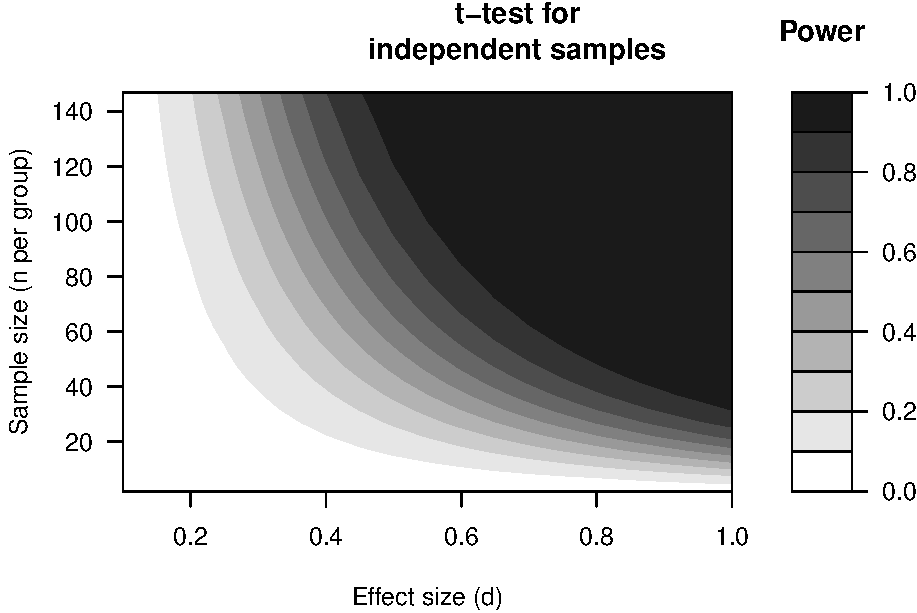
\includegraphics{QMS-EN_files/figure-latex/powercontours-alpha01-1.pdf}
\caption{\label{fig:powercontours-alpha01}Power expressed in contours (see shading), dependent on the standardised effect size (d) and sample size according to a two-sided t-test for unpaired, independent observations, with two-sided significance level alpha=.01.}
\end{figure}

\begin{figure}
\centering
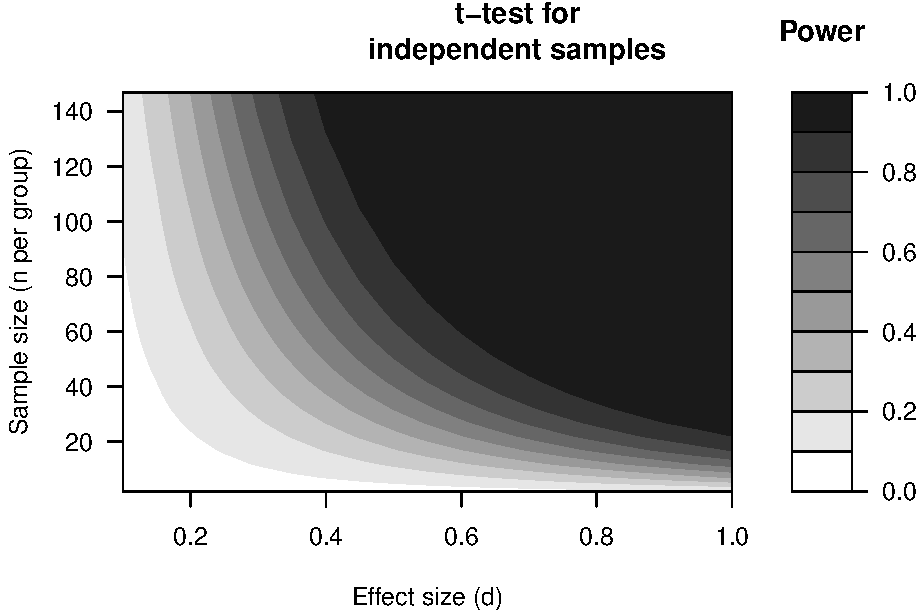
\includegraphics{QMS-EN_files/figure-latex/powercontours-alpha05-1.pdf}
\caption{\label{fig:powercontours-alpha05}Power expressed in contours (see graduation), dependent on the standardised effect size (d) and the sample size (n), according to a two-sided t-test for unpaired, independent observations with significance level alpha=.05.}
\end{figure}

\hypertarget{sec:effectsize-power}{%
\section{Relation between effect size and power}\label{sec:effectsize-power}}

The two figures \ref{fig:powercontours-alpha01} and
\ref{fig:powercontours-alpha05} show that, in general, the larger the effect to be
tested is (more to the right in each figure), the larger the power.
This is also not surprising: a larger effect has
a higher probability of being detected in a statistical test, under
the same circumstances. A moderately large effect of
\(d=.5\), with \(n=30\) observations in each group, only has a probability
of \(.48\) of being detected (if \(\alpha=.05\), Figure \ref{fig:powercontours-alpha05}). On the basis
of a study
with \(n=30\) observations per group is thus actually a gamble
whether a researcher will actually detect such an effect, and
will reject H0. Put otherwise, the probability of a Type I error is
admittedly safely low (\(\alpha=.05\)) but the probability of a Type II error is
more than \(10\times\) as large, and thus dangerously high (\(\beta=.52\)) \citep[Ch.12]{Rose08}.

A larger effect has a higher probability of being detected. A larger
effect of \(d=.8\), for example, results in a power of
\(.86\) with this testing. The probability of a Type II error \(\beta=.14\) here is
admittedly also larger than the probability of a Type I error, but the
proportion \(\beta/\alpha\) is considerably less skewed.

As researchers, we only have an indirect influence on effect size.
We of course have no influence on the true raw difference \(D\) in the
population. For the power, however, the raw difference \(D\) is not
important, but rather the standardised difference \(d=D/s\)
(§\ref{sec:ttest-effectsize}). Thus, if we ensure that the standard
deviation \(s\) decreases, then \(d\) will increase,
and then the power will also increase
(figures~\ref{fig:powercontours-alpha01} and \ref{fig:powercontours-alpha05}),
and we thus have a higher probability
of actually detecting an effect!
With this goal in mind, researchers always strive to neutralise
disrupting influences from all kinds of other factors as much as possible.
After all, the disrupting influences produce extra variability in the observations, and,
with this, a lower power with the statistical testing.

In a well-designed study, we want to determine in advance what
the power will be, and how large the sample should be (see below).
For this we need an estimation of the smallest effect size \(d\)
which we still want to detect
(§\ref{sec:ttest-effectsize}) \citep{Quene10}. To estimate the effect size, firstly,
an estimate of the raw difference \(D\) between the groups or conditions is needed.
Secondly, an estimation is needed of the variability \(s\)
in the observations. These estimations can be largely deduced from
earlier publications, in which the standard deviation
\(s\) is usually reported. If no earlier research reports are available,
then \(s\) can be roughly estimated from some informal
`pilot' observations. Take the difference between the highest and the lowest
(range) of these, divide this range by 4, and use the outcome of this as
a rough estimation for \(s\) \citep{PD08}.

\hypertarget{sec:samplesize-power}{%
\section{Relation between sample size and power}\label{sec:samplesize-power}}

The relation between the sample size \(N\) and the power of a study
is illustrated in
Figure~\ref{fig:powercontours-alpha01} for a strict significance
level \(\alpha=.01\), and in
Figure \ref{fig:powercontours-alpha05} for the most used
significance level \(\alpha=.05\). The figures show that, in general, the larger the
sample gets (further upwards), the larger the power is.
The increase is steeper (power increases more quickly) with larger
effects (right-hand side) than with smaller effects (left-hand side). Put differently:
with small effects, the sample is actually always too small to detect
these small effects with sufficient power. We already saw that in
Example 13.3 (Chapter \ref{ch:testing}).

The two figures \ref{fig:powercontours-alpha01} and
\ref{fig:powercontours-alpha05} are based on the comparison between two groups which are equally large, each with
precisely half of the observations (\(n_1=n_2=N/2\)). That is also most efficient.
The power is based on the \emph{harmonic mean} of \(n_1\) and \(n_2\) (see §\ref{sec:harmonicmean}), and
that harmonic mean is always smaller than the arithmetic mean of those two numbers. It is thus
advisable to ensure that the groups or samples which you compare are approximately equally large.

\begin{center}\rule{0.5\linewidth}{0.5pt}\end{center}

\begin{quote}
\emph{Example 14.1}: In a study, two groups of participants are compared, with \(n_1=10\) and \(n_2=50\)\\
(\(N=n_1+n_2=10+50=60\)). The harmonic mean of \(n_1=10\) and \(n_2=50\) is \(H=17\). This study thus has the same
power as a smaller study with two groups, each of 17 participants, thus 34 participants in total. For this
study, thus, 26 participants more have been investigated (and bothered)
than necessary (see also §\ref{sec:design}) \citep[p.295]{ACA11}.
\end{quote}

\begin{center}\rule{0.5\linewidth}{0.5pt}\end{center}

\hypertarget{sec:significancelevel-power}{%
\section{Relation between significance level and power}\label{sec:significancelevel-power}}

The relation between the significance level \(\alpha\) and the power is
illustrated by the difference between the two figures
\ref{fig:powercontours-alpha01} and
\ref{fig:powercontours-alpha05}. For each combination of effect size
and sample size, the power is lower in
Figure~\ref{fig:powercontours-alpha01} for \(\alpha=.01\) than in
Figure~\ref{fig:powercontours-alpha05} for \(\alpha=.05\). If we choose a higher
significance level \(\alpha\), then the probability of rejecting H0
increases, and thus also the power of correctly rejecting H0 when H0
is untrue (see Table~\ref{tab:H0H1outcomes}).
However, unfortunately, with a high significance
level \(\alpha\), the probability of wrongly rejecting H0 (i.e.~of making a
Type I error) also increases. The investigator
must make a well-considered decision between Type I errors (with
probability \(\alpha\)) and Type II errors (with probability \(\beta\)); as said earlier,
this decision has to depend on the seriousness of (the consequences of) these
two types of errors.

\hypertarget{disadvantages-of-insufficient-power}{%
\section{Disadvantages of insufficient power}\label{disadvantages-of-insufficient-power}}

Unfortunately, many examples can be found of `underpowered' research
in the domain of language and communication. This research has a too small
probability of rejecting H0 when the investigated effect indeed
exists (H0 is not true). Why is that bad \citep{Quene10}?

Firstly, the Type II error which occurs here can have serious consequences:
a treatment method which is actually better is not recognised as such,
a patient is not or wrongly diagnosed, a useful innovation is wrongly pushed
aside. This error hinders the growth of our knowledge and our insight, and hinders
scientific progress (see also
Example 3.2 in Chapter \ref{ch:integrity}).

\begin{figure}
\centering
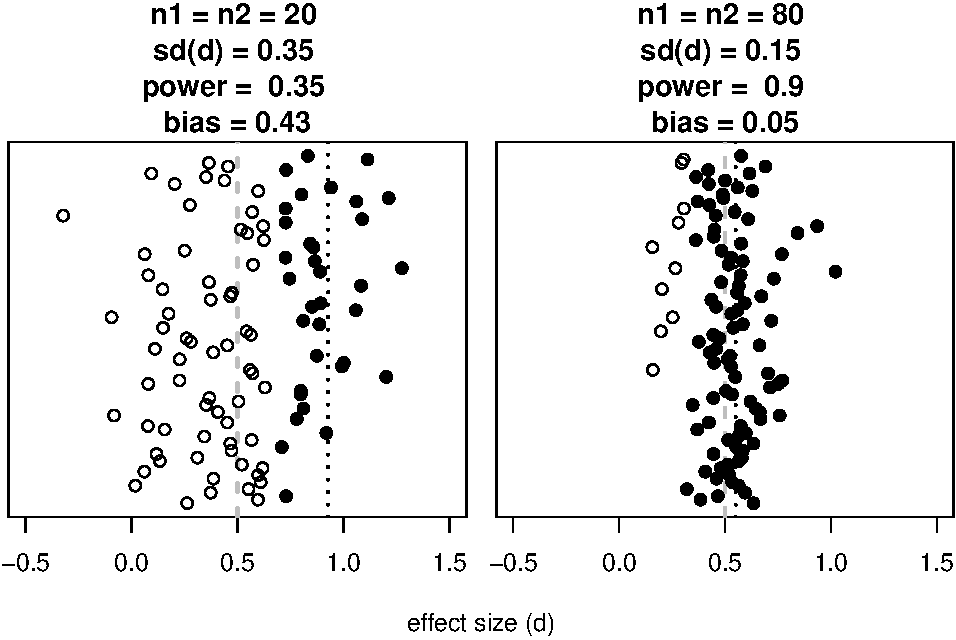
\includegraphics{QMS-EN_files/figure-latex/underpoweredeffectsizes-1.pdf}
\caption{\label{fig:underpoweredeffectsizes}Effect sizes (along the horizontal axis) found in simulated experiments (two-sided t-test for independent observations, alpha=.05), broken down according to sample size (left \(n=20\), right \(n=80\)) and according to testing result (dark symbols: significant; light symbols: not significant). The true effect size between groups is always \(d=0.5\), indicated by the grey dashed line. The mean effect size found from the significant outcomes is referred to with the black dashed line. For each sample size, 100 simulations have been carried out (long vertical axis).}
\end{figure}

The outcomes of simulated experiments with different
sample size, and thus with different power, are summarised
in Figure \ref{fig:underpoweredeffectsizes}. We explain the second disadvantage on the basis of
the somewhat complex figure. In the left panel of Figure
\ref{fig:underpoweredeffectsizes}, we can see that the different
(simulations of) `underpowered' studies show a mixed
picture. Some of these studies do show a significant effect (dark symbols),
and many other studies do not (light symbols).
The mixed picture then usually leads to follow up research, in which
people try to find out \emph{why} the effect does occur in some studies,
and not in others. Might the difference in results be attributable
to differences in stimuli? participants? tasks?
instruments? All that follow up research is \emph{superfluous} though: the mixed
picture from these studies can be explained by the small
power of each study. The needless and superfluous follow up research
costs much time and money (and indirect costs,
see Chapter \ref{ch:integrity}), and comes at the cost of other, more useful
research \citep[p.118]{Schm96}. Put otherwise: one well designed study
with power which is more than sufficient can avoid many needless follow up studies.

The third disadvantage is based on the experience that studies in which
a significant effect is found (dark symbols) have a higher probability
of being reported; this phenomenon is called
`publication bias' or the `file drawer problem'. After all, a positive result
often does get published, whilst a negative result often disappears
into a file drawer. With small power, that leads to the third disadvantage,
namely an overestimation or `bias' of the reported effect size.
In an underpowered study, after all, an effect
must be quite large to be found. In the leftmost panel, we can see that
a significant effect has only been found \(31\times\). The average effect size of these
31 significant outcomes is \(\overline{d_{\textrm{signif}}}=0.90\) (black dashed line), i.e.
a distortion or `bias' of \(0.40\) relative to the actual
\(d=0.50\) (grey dashed line)\footnote{A replication study which does have sufficient power, thus typically finds a smaller effect than the
  original `underpowered' study. The smaller effect found in the replication study is then typically also not
  significant. We then say that the replication study ``fails to replicate'' the effect that was significant in
  the original study - but that was actually a spurious finding.}. In the rightmost panel, we can see that
a significant effect has been found \(91\times\) (thus the power here is sufficient).
The mean effect size of these 91 significant outcomes hardly deviates
from the actual \(d\). Moreover, the standard deviation of the reported
effect size is smaller, and that is again important for later research, meta-studies,
and systematic reviews.

Fourthly, the mixed picture from the different studies, sometimes with significant
outcomes and sometimes without, and with great variation in the reported
effect size, carries the danger that these
outcomes are taken less seriously than `consumers' of
scientific knowledge (practitioners, health insurers, developers,
policy makers, etc.). In this way, these consumers get the impression
that the scientific evidence for this investigated effect is not strong,
and/or that the researchers are in disagreement about whether the effect exists
and if it does, how large it then is \citep{Kolf93} (Figure~\ref{fig:underpoweredeffectsizes}).
This, also hinders scientific progress, and it hinders the use
of scientific insights in societal applications.

To avoid all these objections, researchers have to take into account
the desired power of a study in an early stage. Designing and conducting
a study with insufficient power is after all in opposition with the earlier discussed
ethical and moral principles of diligence and responsibility
(§\ref{sec:integrity-introduction}).

\hypertarget{ch:anova}{%
\chapter{Analysis of variance}\label{ch:anova}}

\hypertarget{sec:introduction}{%
\section{Introduction}\label{sec:introduction}}

This chapter is about an often used statistical analysis, called
analysis of variance (often abbreviated to ANOVA).

The structure of this chapter is as follows. We will begin in §\ref{sec:anova-examples}
with some examples of research studies whose outcomes
can be tested with analysis of variance. The purpose of this section
is to familiarise you with the technique,
with the new terminology, and with the conditions under which this technique
can be used. In §\ref{sec:anova-oneway-explanation}, we will introduce this technique
in an intuitive manner by looking at the thinking behind the test. In
§\ref{sec:anova-oneway-formal} we derive a formal form for the most important
test statistic, the \(F\)-ratio.

\hypertarget{sec:anova-examples}{%
\section{Some examples}\label{sec:anova-examples}}

Just like the \emph{t}-test, analysis of variance is a statistical generalisation
technique, which is to say: an instrument that can be used
when formulating statements about the population characteristics,
on the basis of data taken from samples from these populations.
In the case of the \emph{t}-test and ANOVA, the statements are about
whether or not the means of (two or more) populations are equal.
In this sense, analysis of variance can also be understood as an
expanded version of the \emph{t}-test: we can analyse data
of more than two samples with ANOVA. Moreover, it is possible to include the effects
of multiple independent variables simultaneously in the analysis. This is useful
when we want to analyse data from a factorial design
(§\ref{sec:factorial-designs}).

\begin{center}\rule{0.5\linewidth}{0.5pt}\end{center}

\begin{quote}
\emph{Examples 15.1}: In this example, we investigate the speech tempo or
speed of four groups of speakers, namely originating from the Middle, North,
South and West of the Netherlands. The speech tempo is expressed as the mean
duration of a syllable (in seconds), with the mean taken over an interview of approximately
15 minutes with each speaker \citep{Quene08} \citep{R-hqmisc}.
A shorter mean syllable duration thus corresponds to a faster speaker (cf.~skating, where a faster skater has shorter lap durations). There were 20
speakers per group, but 1 speaker (from the South), who had an extremely high value,
was removed from the sample.
\end{quote}

\begin{center}\rule{0.5\linewidth}{0.5pt}\end{center}

The observed speech tempos per speaker from the above Example 15.1 are summarised
in Table \ref{tab:sylduration} and Figure~\ref{fig:sylduration-boxplot}.

Here, the region of origin is an independent categorial variable or `factor'.
The values of this factor are also referred to as `levels', or in many studies
as `groups' or `conditions'. Each level or each group or condition forms
a `cell' of the design, and the observations from that cell are also
called `replications' (consider why they are called this).
The speech tempo is the dependent variable. The null hypothesis is that the
dependent variable means are equal for all groups, thus
H0: \(\mu_M = \mu_N = \mu_Z = \mu_W\). If we reject H0, then that means
\emph{only} that not all means are equal, but it does \emph{not} mean that each group
mean deviates from each other group mean. For this, a further (post-hoc)
study is necessary; we will return to this later.

\begin{longtable}[]{@{}lccc@{}}
\caption{\label{tab:sylduration} Mean speech tempos, with standard deviation and numbers
of speakers, divided according to region of origin of the speaker (see Example
15.1).}\tabularnewline
\toprule
Region & Mean & s.d. & n\tabularnewline
\midrule
\endfirsthead
\toprule
Region & Mean & s.d. & n\tabularnewline
\midrule
\endhead
Middle & 0.253 & 0.028 & 20\tabularnewline
North & 0.269 & 0.029 & 20\tabularnewline
South & 0.260 & 0.030 & 19\tabularnewline
West & 0.235 & 0.028 & 20\tabularnewline
\bottomrule
\end{longtable}

\begin{figure}
\centering
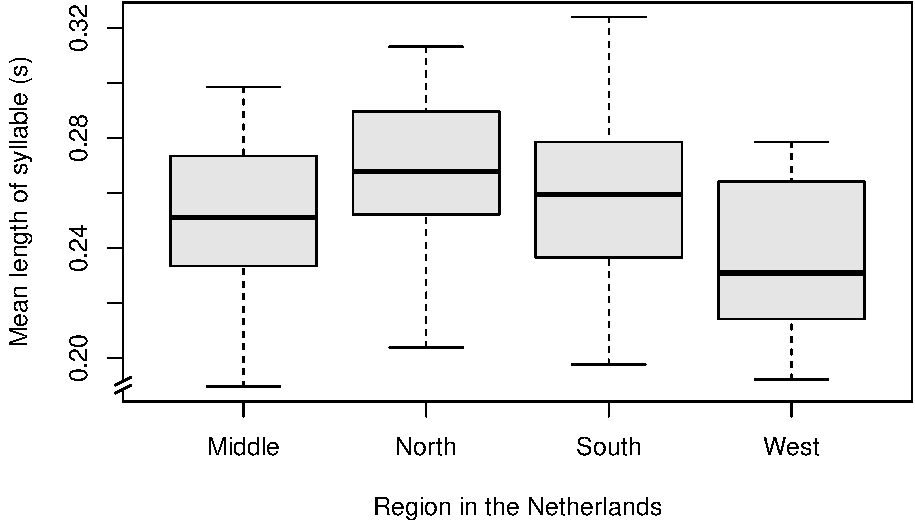
\includegraphics{QMS-EN_files/figure-latex/sylduration-boxplot-1.pdf}
\caption{\label{fig:sylduration-boxplot}Boxplot of the mean length of syllable, split up according to region of origin of the speaker.}
\end{figure}

In order to investigate whether the four populations differ in their average
speech tempo, we could in the first instance conduct \emph{t}-tests for all pairs
of levels. (With 4 levels, that would require 6 tests, see
equation \eqref{eq:choose} with \(n=4\) and \(x=2\)). There are however various
objections to this approach. We will discuss one of these here. For
each test, we use a p-value of \(\alpha=.05\).
We thus have a probability of .95 of a correct decision without a Type I error.
The probability that we will make a correct decision for all 6 tests is
\(.95^6 = .731\) (according to the multiplication principle,
equation \eqref{eq:probability-productrule}).
The joint probability of one or more
Type I error(s) in the 6 tests is thus no longer \(.05\), but has now
increased to \(1-.731 = .265\), more than a quarter!

Analysis of variance now offers the possibility of investigating the
aforementioned null hypothesis on the basis of
a single testing (thus not 6 tests). Analysis of variance can thus be best
characterised as a global testing technique, which is most suitable
if a priori you are not able or do not want to make any specific predictions
about the differences between the populations.

An analysis of variance applied to the scores summarised in
Table~\ref{tab:sylduration}
will lead to the rejection of the null hypothesis: the 4 regional
means are not equal. The differences found are, in all probability, not due to
chance sample fluctuations, but instead to systematic differences between
the groups (\(\alpha=.05\)). Can it now be concluded that the differences
found in speech tempo are \emph{caused} by differences in the origin of the
speaker? Here, restraint is required (see
§\ref{sec:causality}). After all, it cannot be excluded that
the four populations not only differ systematically from each other in speech
tempo, but also in other relevant factors which were not included in the study,
such as health, wealth, or education. We would only be able to exclude these other
factors if we allocated the participants randomly to the selected levels of the
independent variable. However, this is not possible when we are concerned with the
region of origin of the speaker: we can usually assign a speaker (randomly)
to a form of treatment or condition, but not to a region of origin. In fact,
the study in Example 15.1 is thus quasi-experimental.

For our second example, we involve a second factor in the same study
on speech tempo, namely also the speaker's gender.
ANOVA enables us, in one single analysis, to test whether (i) the four
regions differ from each other (H0: \(\mu_M = \mu_N = \mu_Z = \mu_W\)), and
(ii) whether the two genders differ from each other (H0:
\(\mu_\textrm{woman} = \mu_\textrm{man}\)), and (iii) whether the differences
between the regions are the same for both genders (or, put differently, whether
the differences between the genders are the same for all
regions). We call the latter differences the `interaction' between the two factors.

\begin{longtable}[]{@{}ccccc@{}}
\caption{\label{tab:sylduration2way} Mean speech tempos, with standard deviation and
numbers of speakers, divided according to gender and the speaker's region of origin
(see Example 15.1).}\tabularnewline
\toprule
Gender & Region & Mean & s.d. & n\tabularnewline
\midrule
\endfirsthead
\toprule
Gender & Region & Mean & s.d. & n\tabularnewline
\midrule
\endhead
Woman & Middle & 0.271 & 0.021 & 10\tabularnewline
Woman & North & 0.285 & 0.025 & 10\tabularnewline
Woman & South & 0.269 & 0.028 & 9\tabularnewline
Woman & West & 0.238 & 0.028 & 10\tabularnewline
Man & Middle & 0.235 & 0.022 & 10\tabularnewline
Man & North & 0.253 & 0.025 & 10\tabularnewline
Man & South & 0.252 & 0.030 & 10\tabularnewline
Man & West & 0.232 & 0.028 & 10\tabularnewline
\bottomrule
\end{longtable}

The results in Table \ref{tab:sylduration2way} suggest that (i) speakers from the
West speak more quickly than the others, and that (ii) men speak more quickly than
women (!). And (iii) the difference between men and women appears to be smaller
for speakers from the West than for speakers from other regions.

\hypertarget{assumptions-2}{%
\subsection{assumptions}\label{assumptions-2}}

The analysis of variance requires four assumptions which
must be satisfied to use this test; these assumptions match those of the
\emph{t}-test
(§\ref{sec:ttest-assumptions}).

\begin{itemize}
\item
  The data has to be measured on an interval level of measurement (see
  §\ref{sec:interval}).
\item
  All observations have to be independent of each other.
\item
  The scores have to be normally distributed (see
  §\ref{sec:isvarnormaldistributed}).
\item
  The variance of the scores has to be (approximately) equal in
  the scores of the respective groups or conditions (see
  §\ref{sec:variance}).
  The more the samples differ in size, the more serious
  violating this assumption is. It is thus sensible to work with
  equally large, and preferably not too small samples.
\end{itemize}

Summarising: analysis of variance can be used to compare multiple
population means, and to determine the effects of multiple
factors and combinations of factors (interactions).
Analysis of variance does require that data satisfy multiple
conditions.

\hypertarget{one-way-analysis-of-variance}{%
\section{One-way analysis of variance}\label{one-way-analysis-of-variance}}

\hypertarget{sec:anova-oneway-explanation}{%
\subsection{An intuitive explanation}\label{sec:anova-oneway-explanation}}

As stated, we use analysis of variance to investigate whether the
scores of different groups, or those collected under different conditions,
differ from each other. However --- scores \emph{always} differ
from each other, through chance fluctuations between the replications within
each sample. In the preceding chapters, we already encountered
many examples of chance fluctuations within the same sample and within
the same condition. The question then is whether the scores
\emph{between} the different groups (or gathered under different
conditions) differ more from each other than you would expect on the
basis of chance fluctuations \emph{within} each group or cell.

The aforementioned ``differences between scores'' taken together form the
variance of those scores
(§\ref{sec:variance}). For analysis of variance, we divide the total
variance into two parts: firstly, the variance caused by (systematic)
differences \emph{between} groups, and secondly, the variance caused
by (chance) differences \emph{within} groups. If H0 is true,
and if there are thus no differences (in the populations) between the
groups, then we nevertheless expect (in the samples of the groups)
some differences between the mean scores of the groups, be it that
the last mentioned differences will not be greater than
the chance differences within the groups, if H0 is true.
Read this paragraph again carefully.

This approach is illustrated in
Figure \ref{fig:colours-obs}, in which the scores from three experimental
groups (with random assignment of participants to the groups) are shown:
the red, grey and blue group. The scores differ from each other, at least
through chance fluctuations of the scores within
each group. There are probably also systematic differences between (the
mean scores of) the three groups. However, are these systematic
differences now comparatively larger than the chance differences within each
group? If so, then we reject H0.

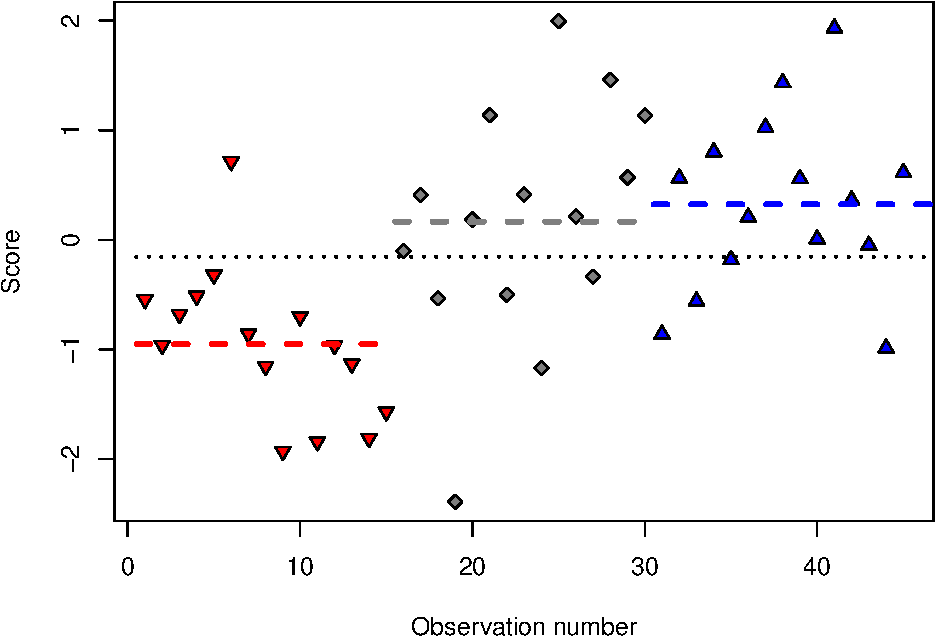
\includegraphics{QMS-EN_files/figure-latex/colours-obs-1.pdf}
The systematic differences \emph{between} the groups correspond with the
differences from the red, grey and blue group means
(dashed lines in Figure \ref{fig:colours-obs}) relative to the mean over
all observations (dotted line). For the first observation, that is a
negative deviation since the score is below the general mean
(dotted line). The chance differences \emph{within} the groups
correspond to the deviation of each observation relative to the
group mean (for the first observation that is thus a positive
deviation, since the score is above the group average of the red
group).

Let us now make the switch from `differences' to `variance'. We then split
the deviation of each observation relative to the general
mean into to two deviations: first, the deviation of the group
mean relative the general mean, and, second, the deviation of
each replication relative to the group mean. These are two pieces of variance
which together form the total variance. Vice versa, we can thus divide
the total variance into two components, which is where the name
`analysis of variance' comes from. (In the next section, we will explain
how these components are calculated, taking into account the number of
observations and the number of groups.)

Dividing the total variance into two variance components is
useful because we can determine the \emph{ratio} between these two parts.
The ratio between the variances is called the \(F\)-ratio, and we use
this ratio to test H0.

\[\textrm{H0}: \textrm{variance between groups} = \textrm{variance within groups}\]

\[\textrm{H0}: F = \frac{\textrm{variance between groups}}{\textrm{variance within groups}} = 1\]

As such, the \(F\)-ratio is a test statistic whose probability distribution
is known if H0 is true. In the example of Figure
\ref{fig:colours-obs}, we find \(F=3.22\), with 3 groups and 45
observations, \(p=.0004\). We thus find a relatively large systematic
variance \emph{between} groups here, compared to the relatively
small chance variance \emph{within} groups: the former variance
(the fraction \(F\)'s numerator) is more than \(3\times\) as large as the
latter variance (the fraction \(F\)'s denominator). The probability
\(p\) of finding this fraction if H0 is true, is exceptionally small,
and we thus reject H0. (In the following section, we will explain how
this probability is determined, again taking into account the number of
observations and the number of groups.) We then speak of a significant effect
of the factor on the dependent variable.

At the end of this section, we repeat the core essence of\\
analysis of variance. We divide the total variance into two parts: the
possible systematic variance between groups or conditions, and the
variance within groups or conditions (i.e.~ever present, chance
fluctuation between replications). The test statistic \(F\) consists of the
proportion between these two variances. We do a one-sided test to see
whether \(F=1\), and reject H0 if \(F>1\) such that the probability
\(P(F|\textrm{H0}) < \alpha\). The mean scores of the groups or conditions
are then in all probability not equal. With this, we do not yet know
which groups differ from each other - for this another further
(post-hoc) analysis is needed
(§\ref{sec:anova-oneway-posthoc} below).

\hypertarget{sec:anova-oneway-formal}{%
\subsection{A formal explanation}\label{sec:anova-oneway-formal}}

For our explanation, we begin with the observed scores. We assume that
the scores are constructed according to a certain statistical model, namely
as the sum of the population mean (\(\mu\)), a systematic
effect (\(\alpha_j\)) of the \(j\)'the condition or group (over \(k\) conditions
or groups), and a chance effect (\(e_{ij}\)) for the \(i\)'the replication within
the \(j\)'the condition or group (over \(N\) replications in
total). In formula:
\[x_{ij} = \mu + \alpha_{j} + e_{ij}\]
Here too, we thus again analyse each score in a systematic part and
a chance part. This is the case not only for the scores themselves, but also
for the deviations of each score relative to the total mean
(see §\ref{sec:anova-oneway-explanation}).

Thus, three variances are of interest. Firstly, the total
variance (see equation
\eqref{eq:variance}, abbreviated to \texttt{t}) over all \(N\)
observations from all groups or conditions together:
\begin{equation}
  \label{eq:MStotal}
    s^2_t = \frac{ \sum (x_{ij} - \overline{x})^2 } {N-1}
\end{equation}
Secondly the variance `between' (abbreviated to \texttt{b}) the groups
or conditions:
\begin{equation}
  \label{eq:MSbetween}
    s^2_b = \frac{ \sum_{j=1}^{j=k} n_j (\overline{x_j} - \overline{x})^2 } {k-1}
\end{equation}
and, thirdly, the variance `within' (shortened to \texttt{w}) the groups or
conditions:
\begin{equation}
  \label{eq:MSwithin}
    s^2_w = \frac{ \sum_{j=1}^{j=k} \sum_i (x_{ij} - \overline{x_j})^2 } {N-k}
\end{equation}

In these comparisons, the \emph{numerators} are formed from the sum of
the squared deviations (`sums of squares', shortened to \texttt{SS}). In the
previous section, we indicated that the deviations add up to each other,
and that then is also the case for the summed and squared
deviations:
\begin{align}
  \label{eq:SStotal}
    { \sum (x_{ij} - \overline{x})^2 } &= 
    { \sum_{j=1}^{j=k} n_j (\overline{x_j} - \overline{x})^2 } + 
    { \sum_{j=1}^{j=k} \sum_i (x_{ij} - \overline{x_j})^2 } \\
    \textrm{SS}_t &= \textrm{SS}_b + \textrm{SS}_w
\end{align}

The
\emph{numerators} of the variances are formed from the degrees of freedom
(abbreviated \texttt{df}, see
§\ref{sec:ttest-freedomdegrees}). For the variance between
groups \(s^2_b\), that is the number of groups or conditions, minus 1 (\(k-1\)).
For the variance within groups \(s^2_w\), that is the number of observations,
minus the number of groups (\(N-k\)). For the total variance, that is the
number of observations minus 1 (\(N-1\)). The degrees of freedom of the
deviations also add up to each other:
\begin{align}
  \label{eq:dftotal1}
    { (N-1) } &= { (k-1) } + { (N-k) } \\
    \textrm{df}_t &= \textrm{df}_b + \textrm{df}_w
\end{align}

The above fractions which describe the variances \(s^2_t\), \(s^2_b\) and \(s^2_w\),
are also referred to as the `mean squares' (shortened to \texttt{MS}).
\(\textrm{MS}_{t}\) is by definition equal to the `normal' variance
\(s^2_x\) (see the identical equations
\eqref{eq:variance} and
\eqref{eq:MStotal}).

The test statistic \(F\) is defined as the ratio of the two
variance components defined above:
\begin{equation}
  \label{eq:Fratio}
    F = \frac{ s^2_b } { s^2_w }
\end{equation}
with not one but two
degrees of freedom, resp. \((k-1)\) for the numerator and \((N-k)\) for the denominator.

You can determine the p-value \(p\) which belongs with the
\(F\) found using a table, but we usually conduct an
analysis of variance using a computer, and it then also calculates the
p-value.

The results of an analysis of variance are summarised in a fixed format
in a so-called ANOVA table, like
Table \ref{tab:colours-anova}. This contains the most important
information summarised. However, the whole table can also be summarised in
one sentence, see Example 15.2.

\begin{longtable}[]{@{}lccccc@{}}
\caption{\label{tab:colours-anova} Summary of analysis of variance of the observations in Figure \ref{fig:colours-obs}.}\tabularnewline
\toprule
Variance Source & df & SS & MS & \(F\) & \(p\)\tabularnewline
\midrule
\endfirsthead
\toprule
Variance Source & df & SS & MS & \(F\) & \(p\)\tabularnewline
\midrule
\endhead
Group & 2 & 14.50 & 7.248 & 9.356 & 0.0004\tabularnewline
(within) & 42 & 32.54 & 0.775 & &\tabularnewline
\bottomrule
\end{longtable}

\begin{center}\rule{0.5\linewidth}{0.5pt}\end{center}

\begin{quote}
\emph{Example 15.2}:
The mean scores are not equal for the red, grey and blue group
{[}\(F(2,42) = 9.35\), \(p = .0004\), \(\omega^2 = 0.28\){]}.
\end{quote}

\begin{center}\rule{0.5\linewidth}{0.5pt}\end{center}

\hypertarget{sec:anova-oneway-effectsize}{%
\subsection{Effect size}\label{sec:anova-oneway-effectsize}}

Just like with the \(t\)-test, it is not only important to make a binary decision
about H0, but it is at least equally important to know how large
the observed effect is (see also
§\ref{sec:ttest-effectsize}). This effect size for
analysis of variance can be expressed in different measures, of which we will
discuss two (this section is based on \citet{KL00}; see also \citet{Olej03}).

The simplest measure is the so-called \(\eta^2\) (``eta
squared''), the proportion of the total SS which can be attributed to the
differences between the groups or conditions: \[\label{eq:etasq}
    \eta^2 = \frac{ \textrm{SS}_b } { \textrm{SS}_t }\] The effect size
\(\eta^2\) is a proportion between 0 and 1, which indicates how much of the
variance in the \emph{sample} can be assigned to the independent
variable.

The second measure for effect size with analysis of variance is the so-called
\(\omega^2\) (``omega squared''):
\begin{equation}
  \label{eq:omegasq}
    \omega^2 = \frac{ \textrm{SS}_b - (k-1) \textrm{MS}_w} { \textrm{SS}_t + \textrm{MS}_w }
\end{equation}
The effect size \(\omega^2\) is also a proportion; this is an estimation
of the proportion of the variance in the \emph{population} which can be attributed
to the independent variable, where the estimation is of course based
on the investigated sample. As we are generally more interested in
generalisation to the population than to the sample, we prefer \(\omega^2\)
as the measure for the effect size.

We should not only report the \(F\)-ratio, degrees of freedom,
and p-values, but also the effect size (see
Example 15.2 above).

\begin{quote}
``It is not enough to report
\(F\)-ratios and whether they are statistically significant. We must know
how strong relations are. After all, with large enough \(N\)s, \(F\)- and
\(t\)-ratios can almost always be statistically significant. While often
sobering in their effect, especially when they are low, coefficients of
association of independent and dependent variables {[}i.e., effect size
coefficients{]} are \emph{indispensable} parts of research results'' \citep[ p.327, emphasis added]{KL00}.
\end{quote}

\hypertarget{sec:anova-oneway-planned}{%
\subsection{Planned comparisons}\label{sec:anova-oneway-planned}}

In Example 15.2 (see
Figure \ref{fig:colours-obs}), we investigated the differences between
scores from the red, grey and blue groups. The null hypothesis which was tested
was H0:
\(\mu_\textrm{red} = \mu_\textrm{grey} = \mu_\textrm{blue}\).
However, it is also quite possible that a researcher already has
certain ideas about the differences between groups, and is looking in a
\emph{focused} manner for certain differences, and wants to actually ignore other
differences. The planned comparisons are also called `contrasts'.

Let us assume for the same example that the researcher already expects,
from previous research, that the red and blue group scores will differ from
each other. The H0 above is then no longer interesting to investigate, since
we expect in advance that we will reject H0. The researcher now wants to know
in a planned way (1) whether the red group scores lower than the other two groups,
(H0: \(\mu_\textrm{red} = (\mu_\textrm{grey}+\mu_\textrm{blue})/2\)),
and (2)
whether the grey and blue groups differ from each other (H0:
\(\mu_\textrm{grey} = \mu_\textrm{blue}\))
\footnote{If (1) red does differ from grey and blue, and if (2) grey and blue
  also differ from each other, then this implies that red differs from grey (a new
  finding) and that red differs from blue (we already knew that).}.

The factor `group' or `colour' has 2 degrees of freedom, and that means that we
can make precisely 2 of such planned comparisons or `contrasts' which are
independent of each other. Such independent contrasts
are called `orthogonal'.

In an analysis of variance with planned comparisons, the variance between
groups or conditions is divided even further, namely into the planned
contrasts such as the two above (see
Table~\ref{tab:colours-anova-contrast}). We omit further explanation
about planned comparisons but our advice is to make
smart use of these planned comparisons when possible. Planned comparisons are advised whenever
you can formulate a more
specific null hypothesis than H0: ``the mean scores are equal
in all groups or conditions''. We can make planned statements
about the differences between the groups in our example:

\begin{center}\rule{0.5\linewidth}{0.5pt}\end{center}

\begin{quote}
\emph{Example 15.3}:
The mean score of the red
group is significantly lower than that from the two other groups combined
{[}\(F(1,42)=18.47, p=.0001, \omega^2=0.28\){]}. The mean score is
almost the same for the grey and blue group
{[}\(F(1,42)<1, \textrm{n.s.}, \omega^2=0.00\){]}.
This implies that the red group achieves significantly lower scores than the
grey group and than the blue group.
\end{quote}

\begin{center}\rule{0.5\linewidth}{0.5pt}\end{center}

\begin{longtable}[]{@{}lccccc@{}}
\caption{\label{tab:colours-anova-contrast} Summary of analysis of variance of the observations in Figure \ref{fig:colours-obs}, with planned contrasts between groups.}\tabularnewline
\toprule
Variance source & df & SS & MS & \(F\) & \(p\)\tabularnewline
\midrule
\endfirsthead
\toprule
Variance source & df & SS & MS & \(F\) & \(p\)\tabularnewline
\midrule
\endhead
Group & 2 & 14.50 & 7.248 & 9.356 & 0.0004\tabularnewline
~~Group, contrast 1 & 1 & 14.31 & 14.308 & 18.470 & 0.0001\tabularnewline
~~Group, contrast 2 & 1 & 0.19 & 0.188 & 0.243 & 0.6248\tabularnewline
(within) & 42 & 32.54 & 0.775 & &\tabularnewline
\bottomrule
\end{longtable}

The analysis of variance with planned comparisons can thus be used
if you already have planned (a priori) hypotheses over differences between
certain (combinations of) groups or conditions. ``A priori'' means that these
hypotheses (contrasts) are formulated before the observations have been made.
These hypotheses can be based on theoretical considerations, or on
previous research results.

\hypertarget{orthogonal-contrasts}{%
\subsubsection{Orthogonal contrasts}\label{orthogonal-contrasts}}

Each contrast can be expressed in the form of weights for each
condition. For the contrasts discussed above, that can be done
in the form of the following weights:

\begin{longtable}[]{@{}ccc@{}}
\toprule
Condition & Contrast 1 & Contrast 2\tabularnewline
\midrule
\endhead
~~Red & -1 & 0\tabularnewline
~~Grey & +0.5 & -1\tabularnewline
~~Blue & +0.5 & +1\tabularnewline
\bottomrule
\end{longtable}

The H0 for contrast 2 (\(\mu_\textrm{grey} = \mu_\textrm{blue}\)) can be
expressed in weights as follows:
\(\textrm{C2} = 0\times \mu_\textrm{red} -1 \times \mu_\textrm{grey} +1 \times \mu_\textrm{blue} = 0\).

To determine whether two contrasts are orthogonal, we multiply
their respective weights for each condition (row):\\
\(( (-1)(0), (+0.5)(-1), (+0.5)(+1) )= (0, -0.5, +0.5)\).\\
We then sum all these products:
\(0 -0.5 + 0.5 = 0\).\\
If the sum of these products is null, then the two
contrasts are orthogonal.

\hypertarget{sec:anova-oneway-posthoc}{%
\subsection{Post-hoc comparisons}\label{sec:anova-oneway-posthoc}}

In many studies, a researcher has no idea about the expected differences
between the groups or conditions. Only after the analysis of variance,
\emph{after} a significant effect has been found, does the researcher decide
to inspect more closely which conditions differ from each other. We speak
then of \emph{post hoc} comparisons, ``suggested by the data'' \citep[ p.200]{MD04}.
When doing so, we have to work conservatively, precisely because
after the analysis of variance we might already suspect that some
comparisons will yield a significant result,
i.e., the null hypotheses are not neutral.

There are many dozens of statistical tests for post hoc
comparisons. The most important difference is their degree of conservatism
(tendency not to reject H0) vs.~liberalism (tendency to indeed reject H0).
Additionally, some tests are better equipped
for pairwise comparisons between conditions (like contrast 2 above) and
others better equipped for complex comparisons
(like contrast 1 below). And the tests differ in the assumptions
which they make about the variances in the cells.

Here, we will mention one test
for post hoc comparisons between pairs of conditions: \emph{Tukey's
Honestly Significant Difference}, abbreviated to Tukey's HSD. This test
occupies a good middle ground between being too conservative and too liberal. An
important characteristic of the Tukey HSD test is that the family-wise
error (the \emph{collective} p-value) over all pairwise comparisons together
is equal to the indicated p-value
\(\alpha\) (see §\ref{sec:anova-examples}). The Tukey HSD test results in
a 95\% confidence interval for the difference between two conditions,
and/or in a \(p\)-value for the difference between two conditions.

\hypertarget{spss-12}{%
\subsection{SPSS}\label{spss-12}}

\hypertarget{preparation}{%
\subsubsection{preparation}\label{preparation}}

We will use the data in the file \texttt{data/kleurgroepen.txt}; this data is also shown in Figure \ref{fig:colours-obs}.
Read first the required data, and check this:

\begin{verbatim}
File > Import Data > Text Data...
\end{verbatim}

Select \texttt{Files\ of\ type:\ Text} and select the file
\texttt{data/kleurgroepen.txt}. Confirm with \texttt{Open}.\\
The names of variables can be found in line 1. The decimal symbol is
the full stop (period). The data starts on line 2. Each line is an observation.
The delimiter used between the variables is a space. The text is between
double quotation marks. You do not need to define the variables further,
the standard options of SPSS work well here.\\
Confirm the last selection screen with \texttt{Done}. The data will
then be read in.

Examine whether the responses are normally distributed, using the
techniques from Part II of this textbook (especially
§\ref{sec:isvarnormaldistributed}).

We cannot test in advance in SPSS whether the variances in the three groups
are equal, as required for the analysis of variance. We will do that at the same
time as the analysis of variance itself.

\hypertarget{anova}{%
\subsubsection{ANOVA}\label{anova}}

In SPSS, you can conduct an analysis of variance in several
different ways. We
will use a generally applicable approach here, where we indicate that there
is one dependent variable in play.\\

\begin{verbatim}
Analyze > General Linear Model > Univariate...
\end{verbatim}

Select \texttt{score} as dependent variable (drag to the panel
``Dependent variable'').\\
Select \texttt{kleur} (the Dutch variable name for colour of the group) as independent variable (drag to the panel ``Fixed
Factor(s)'').\\
Select \texttt{Model...} and then \texttt{Full\ factorial} model, \texttt{Type\ I} Sum
of squares, and tick: \texttt{Include\ intercept\ in\ model}, and confirm with
\texttt{Continue}.\\
Select \texttt{Options...} and ask for means for the conditions
of the factor \texttt{colour} (drag to the Panel ``Display Means for''). Cross:
\texttt{Estimates\ of\ effect\ size} and \texttt{Homogeneity\ tests}, and confirm again with
\texttt{Continue}.\\
Confirm all options with \texttt{OK}.

In the output, we find first the outcome of Levene's test on equal
variances (homogeneity of variance) which gives no reason to reject
H0. We can thus conduct an analysis of variance.

Then, the analysis of variance is summarised in a table like Table
\ref{tab:colours-anova}, where the effect size is also stated in
the form of \texttt{~Partial\ eta\ square}.
As explained above, it would be better, however, to report
\(\omega^2\), but you do have to calculate that yourself!

\hypertarget{planned-comparison}{%
\subsubsection{planned comparison}\label{planned-comparison}}

For an analysis of variance with planned comparisons, we have to
indicate the desired contrasts for the factor \texttt{kleur} (the Dutch variable name for colour of the group).
However, the method
is different to the above. We cannot set the planned contrasts in SPSS
via the menu system which we used until now. Here, we instead have
to get to work ``under the bonnet''!\\
First repeat the instructions above but, instead of confirming everything,
you should now select the button \texttt{Paste}. Then, a so-called Syntax window
will be opened (or activated, if it was already open). Within it, you
will see the SPSS command that you built via the menu.\\
We are going to edit this command in order to indicate our own, special
contrasts. When specifying the contrasts, we do have to take into
account the \emph{alphabetic} order of the conditions: blue, grey,
red.\\
The command in the Syntax window should eventually look like the one
below, after you have added the line \texttt{/CONTRAST}. The command
must be terminated with a full stop.\\

\begin{verbatim}
UNIANOVA score BY colour
  /METHOD=SSTYPE(1)
  /INTERCEPT=INCLUDE
  /EMMEANS=TABLES(colour) 
  /PRINT=ETASQ HOMOGENEITY
  /CRITERIA=ALPHA(.05)
  /DESIGN=colour
  /CONTRAST(colour)=special(0.5 0.5 -1, 1 -1 0).
\end{verbatim}

Place the cursor somewhere between the word \texttt{UNIANOVA} and the terminating
full stop, and then click on the large green arrow to the right (\texttt{Run\ Selection})
in the Syntax window's menu.

The output provides the significance and the confidence interval
of the tested contrast for each contrast. The first contrast
is indeed significant (\texttt{Sig.\ .000}, report as \(p<.001\), see
§\ref{sec:plargerthannull}), and the second is not, see
Table \ref{tab:colours-anova-contrast}.

\hypertarget{post-hoc-comparison}{%
\subsubsection{post hoc comparison}\label{post-hoc-comparison}}

First repeat the instructions above.\\
Select the button \texttt{Post\ Hoc...}, and select the factor \texttt{kleur}
(the Dutch variable name for colour of the group) (move this term to the window ``Post Hoc Tests for:'').
Tick: \texttt{Tukey}, and then \texttt{Continue}. Confirm all options with \texttt{OK}.

For each pairwise comparison, we see the difference, the
standard error, and the Lower Bound and Upper Bound of the 95\%
confidence interval of that difference. If that interval does \emph{not}
include null then the difference between the two groups or conditions is
thus probably not equal to null. The corrected p-value according to Tukey's
HSD test is also provided in the third column. We can see that red
differs from blue, that red differs from grey, and that the scores of the
grey and blue groups do not differ.

\hypertarget{r-15}{%
\subsection{R}\label{r-15}}

\hypertarget{preparation-1}{%
\subsubsection{preparation}\label{preparation-1}}

Read firstly the necessary data, and check this:

\begin{Shaded}
\begin{Highlighting}[]
\CommentTok{\# same data as used in Fig.15.2}
\NormalTok{colourgroups \textless{}{-}}\StringTok{ }\KeywordTok{read.table}\NormalTok{( }\StringTok{"data/kleurgroepen.txt"}\NormalTok{, }
                            \DataTypeTok{header=}\OtherTok{TRUE}\NormalTok{, }\DataTypeTok{stringsAsFactors=}\OtherTok{TRUE}\NormalTok{ )}
\end{Highlighting}
\end{Shaded}

Examine whether the responses are normally distributed, using
the techniques from Part II of this textbook (especially
§\ref{sec:isvarnormaldistributed}).

Investigate whether the variances in the three groups are equal, as required
for analysis of variance. The H0 which we are testing is:
\(s^2_\textrm{red} = s^2_\textrm{grey} = s^2_\textrm{blue}\). We
test this H0 using Bartlett's test.

\begin{Shaded}
\begin{Highlighting}[]
\KeywordTok{bartlett.test}\NormalTok{( }\DataTypeTok{x=}\NormalTok{colourgroups}\OperatorTok{$}\NormalTok{score, }\DataTypeTok{g=}\NormalTok{colourgroups}\OperatorTok{$}\NormalTok{kleur )}
\end{Highlighting}
\end{Shaded}

\begin{verbatim}
## 
##  Bartlett test of homogeneity of variances
## 
## data:  colourgroups$score and colourgroups$kleur
## Bartlett's K-squared = 3.0941, df = 2, p-value = 0.2129
\end{verbatim}

\hypertarget{anova-1}{%
\subsubsection{ANOVA}\label{anova-1}}

\begin{Shaded}
\begin{Highlighting}[]
\KeywordTok{summary}\NormalTok{( }\KeywordTok{aov}\NormalTok{( score}\OperatorTok{\textasciitilde{}}\NormalTok{kleur, }\DataTypeTok{data=}\NormalTok{colourgroups) {-}\textgreater{}}\StringTok{ }\NormalTok{m01 ) }\CommentTok{\# see Table 15.3}
\end{Highlighting}
\end{Shaded}

\begin{verbatim}
##             Df Sum Sq Mean Sq F value   Pr(>F)    
## kleur        2  14.50   7.248   9.356 0.000436 ***
## Residuals   42  32.54   0.775                     
## ---
## Signif. codes:  0 '***' 0.001 '**' 0.01 '*' 0.05 '.' 0.1 ' ' 1
\end{verbatim}

\hypertarget{R:omega-square}{%
\subsubsection{effect size}\label{R:omega-square}}

\begin{Shaded}
\begin{Highlighting}[]
\CommentTok{\# own function to calculate omega2, see comparison (15.7) in the main text,}
\CommentTok{\# for effect called \textasciigrave{}term\textasciigrave{} in summary(\textasciigrave{}model\textasciigrave{})}
\NormalTok{omegasq \textless{}{-}}\StringTok{ }\ControlFlowTok{function}\NormalTok{ ( model, term ) \{   }
\NormalTok{     mtab \textless{}{-}}\StringTok{ }\KeywordTok{anova}\NormalTok{(model)}
\NormalTok{     rterm \textless{}{-}}\StringTok{ }\KeywordTok{dim}\NormalTok{(mtab)[}\DecValTok{1}\NormalTok{] }\CommentTok{\# resid term}
     \KeywordTok{return}\NormalTok{( (mtab[term,}\DecValTok{2}\NormalTok{]}\OperatorTok{{-}}\NormalTok{mtab[term,}\DecValTok{1}\NormalTok{]}\OperatorTok{*}\NormalTok{mtab[rterm,}\DecValTok{3}\NormalTok{]) }\OperatorTok{/}\StringTok{ }
\StringTok{             }\NormalTok{(mtab[rterm,}\DecValTok{3}\NormalTok{]}\OperatorTok{+}\KeywordTok{sum}\NormalTok{(mtab[,}\DecValTok{2}\NormalTok{])) )}
\NormalTok{\}}
\CommentTok{\# variable kleur=colour is the term to inspect}
\KeywordTok{omegasq}\NormalTok{( m01, }\StringTok{"kleur"}\NormalTok{ ) }\CommentTok{\# call function with 2 arguments}
\end{Highlighting}
\end{Shaded}

\begin{verbatim}
## [1] 0.2708136
\end{verbatim}

\hypertarget{planned-comparison-1}{%
\subsubsection{planned comparison}\label{planned-comparison-1}}

When specifying the contrasts, we have to take into account the
\emph{alphabetic} ordering of the conditions: \emph{blue, grey, red}.
Note that the predictor is named \texttt{kleur} which is the Dutch term for colour of the group).

\begin{Shaded}
\begin{Highlighting}[]
\CommentTok{\# make matrix of two orthogonal contrasts (per column, not per row) }
\NormalTok{conmat \textless{}{-}}\StringTok{ }\KeywordTok{matrix}\NormalTok{( }\KeywordTok{c}\NormalTok{(.}\DecValTok{5}\NormalTok{,.}\DecValTok{5}\NormalTok{,}\OperatorTok{{-}}\DecValTok{1}\NormalTok{, }\OperatorTok{+}\DecValTok{1}\NormalTok{,}\OperatorTok{{-}}\DecValTok{1}\NormalTok{,}\DecValTok{0}\NormalTok{), }\DataTypeTok{byrow=}\NormalTok{F, }\DataTypeTok{nrow=}\DecValTok{3}\NormalTok{ )}
\KeywordTok{dimnames}\NormalTok{(conmat)[[}\DecValTok{2}\NormalTok{]] \textless{}{-}}\StringTok{ }\KeywordTok{c}\NormalTok{(}\StringTok{".R.GB"}\NormalTok{,}\StringTok{".0G.B"}\NormalTok{) }\CommentTok{\# (1) R vs G+B, (2) G vs B }
\KeywordTok{contrasts}\NormalTok{(colourgroups}\OperatorTok{$}\NormalTok{kleur) \textless{}{-}}\StringTok{ }\NormalTok{conmat }\CommentTok{\# assign contrasts to factor}
\KeywordTok{summary}\NormalTok{( }\KeywordTok{aov}\NormalTok{( score}\OperatorTok{\textasciitilde{}}\NormalTok{kleur, }\DataTypeTok{data=}\NormalTok{colourgroups) {-}\textgreater{}}\StringTok{ }\NormalTok{m02 ) }
\end{Highlighting}
\end{Shaded}

\begin{verbatim}
##             Df Sum Sq Mean Sq F value   Pr(>F)    
## kleur        2  14.50   7.248   9.356 0.000436 ***
## Residuals   42  32.54   0.775                     
## ---
## Signif. codes:  0 '***' 0.001 '**' 0.01 '*' 0.05 '.' 0.1 ' ' 1
\end{verbatim}

\begin{Shaded}
\begin{Highlighting}[]
\CommentTok{\# output is necessary for omega2}
\CommentTok{\# see https://blogs.uoregon.edu/rclub/2015/11/03/anova{-}contrasts{-}in{-}r/}
\KeywordTok{summary.aov}\NormalTok{( m02, }\DataTypeTok{split=}\KeywordTok{list}\NormalTok{(}\DataTypeTok{kleur=}\KeywordTok{list}\NormalTok{(}\DecValTok{1}\NormalTok{,}\DecValTok{2}\NormalTok{)) )}
\end{Highlighting}
\end{Shaded}

\begin{verbatim}
##             Df Sum Sq Mean Sq F value   Pr(>F)    
## kleur        2  14.50   7.248   9.356 0.000436 ***
##   kleur: C1  1  14.31  14.308  18.470 0.000100 ***
##   kleur: C2  1   0.19   0.188   0.243 0.624782    
## Residuals   42  32.54   0.775                     
## ---
## Signif. codes:  0 '***' 0.001 '**' 0.01 '*' 0.05 '.' 0.1 ' ' 1
\end{verbatim}

When we have planned contrasts, the previously constructed function \texttt{omegasq} can no longer be used (and neither can the previously provided formula). We now have to calculate the \(\omega^2\) by hand using the output from the summary of model \texttt{m02}:

\begin{Shaded}
\begin{Highlighting}[]
\NormalTok{(}\FloatTok{14.308}\DecValTok{{-}1}\OperatorTok{*}\FloatTok{0.775}\NormalTok{)}\OperatorTok{/}\NormalTok{(}\FloatTok{0.775+14.308+0.19+32.54}\NormalTok{) }\CommentTok{\# 0.2830402}
\end{Highlighting}
\end{Shaded}

\begin{verbatim}
## [1] 0.2830402
\end{verbatim}

\begin{Shaded}
\begin{Highlighting}[]
\NormalTok{(}\FloatTok{0.188}\DecValTok{{-}1}\OperatorTok{*}\FloatTok{0.775}\NormalTok{)}\OperatorTok{/}\NormalTok{(}\FloatTok{0.775+14.308+0.19+32.54}\NormalTok{) }\CommentTok{\# rounded off 0.00}
\end{Highlighting}
\end{Shaded}

\begin{verbatim}
## [1] -0.012277
\end{verbatim}

\hypertarget{post-hoc-comparisons}{%
\subsubsection{post hoc comparisons}\label{post-hoc-comparisons}}

\begin{Shaded}
\begin{Highlighting}[]
\KeywordTok{TukeyHSD}\NormalTok{(m02)}
\end{Highlighting}
\end{Shaded}

\begin{verbatim}
##   Tukey multiple comparisons of means
##     95% family-wise confidence level
## 
## Fit: aov(formula = score ~ kleur, data = colourgroups)
## 
## $kleur
##                  diff        lwr        upr     p adj
## grey50-blue -0.158353 -0.9391681  0.6224622 0.8751603
## red-blue    -1.275352 -2.0561668 -0.4945365 0.0007950
## red-grey50  -1.116999 -1.8978139 -0.3361835 0.0033646
\end{verbatim}

For each pair, we see the difference, and the Lower Bound (\texttt{lwr}) and
the Upper Bound (\texttt{upr}) of the 95\% confidence interval
of the difference. If that interval does \emph{not} include null, then
the difference between the two groups or conditions is thus probably not
equal to null. The corrected p-value according to
Tukey's HSD test is also given in the last column.
Again, we see that red differs from grey, that red differs from
blue, and that the grey and blue scores do not differ.

\hypertarget{two-way-analysis-of-variance}{%
\section{Two-way analysis of variance}\label{two-way-analysis-of-variance}}

In §\ref{sec:anova-examples}, we already gave an example
of a research study with two factors which were investigated in one analysis
of variance. In this way, we can investigate (i) whether there is a
main effect from the first factor (e.g.~the speaker's region of origin),
(ii) whether there is a main effect from the second factor (e.g.~
speaker gender), and (iii) whether there is an interaction effect.
A such interaction implies that the differences between conditions of
one factor are not the same
for the conditions of the other factor, or put otherwise, that a cell's mean
score deviates from the predicted value based on the two main effects.

\hypertarget{an-intuitive-explanation}{%
\subsection{An intuitive explanation}\label{an-intuitive-explanation}}

In many studies, we are interested in the \emph{combined} effects
of two or more factors. In
Table~\ref{tab:sylduration2way}, we already saw mean speech tempos,
split up according to the speaker's region of origin and sex.
If the differences between the regions are different for men compared with
women, or put differently, if the differences between men and women are
different for the different regions then we speak of an interaction. By adding
a second factor into the study, we thus have to deal with a third factor,
namely the interaction between
the first and second factor
\footnote{If we add more factors then the situation quickly becomes confusing.
  With three main effects, there are already 3 two-way interactions plus 1 three-way
  interaction. With four main effects, there are already 6 two-way interactions, plus
  4 three-way interactions, plus 1 four-way interaction.}.

If a significant interaction is present then we can no longer make
general statements about the main effect we are concerned with. After all, the
impact of a main effect is also dependent on the interaction with
(an) other main effect(s), as can be seen in
Figure~\ref{fig:drakebenelheni2003fig2} (§\ref{sec:factorial-designs}).
The listener group's scores are \emph{on average}
not higher compared with those of the other groups,
and the scores are also \emph{on average} not higher in one condition than in the other.
The main effects are thus not significant --- but their interaction
on the other hand is indeed significant. In general, interaction occurs when the effect of one factor varies depending on the different levels of another factor.
In this example of two-way interaction, the effect of one factor is in opposite directions for the two levels of the other factor.

\hypertarget{a-formal-explanation}{%
\subsection{A formal explanation}\label{a-formal-explanation}}

We again assume that the scores have been built up according to
a statistical model, namely as the sum of the population mean
\(\mu\), a systematic effect \(\beta_k\) of the \(k\)'the condition of
factor B, a systematic effect \((\alpha\beta)_{jk}\) of the combination
of conditions \((j,k)\) of factors A and B, and a chance effect
\(e_{ijk}\) for the \(i\)'the replication within the \(jk\)'the cell. In formula:

\[x_{ijk} = \mu + \alpha_{j} + \beta_{k} + (\alpha\beta)_{jk} + e_{ijk}\]

In the one-way analysis of variance the total `sums of squares' is split up
into two components, namely between and within conditions (see
equation \eqref{eq:SStotal}).
With the two-way analysis of variance, there are now however
\emph{four} components:
\begin{align}
  \label{eq:SStotal2way}
    { \sum (x_{ijk} - \overline{x})^2 } = &  { \sum_j n_j (\bar{x}_j - \bar{x})^2 } + \\ 
    & { \sum_k n_k (\bar{x}_k - \bar{x})^2 } +  \\
    & { \sum_j \sum_k n_{jk} (\bar{x}_{jk} - \bar{x}_j - \bar{x}_k + \bar{x})^2 } + \\
    & { \sum_i \sum_j \sum_k (x_{ijk} - \bar{x}_{jk})^2 } 
\end{align}

The degrees of freedom of these sums of squares also add up to each other
again:
\begin{align}
  \label{eq:dftotal2}
    { (N-1) } &= (A-1) &+ (B-1) &+ (A-1)(B-1) &+ (N-AB) \\
    \textrm{df}_t &= \textrm{df}_A &+ \textrm{df}_B &+ \textrm{df}_{AB} &+ \textrm{df}_w
\end{align}

Just like with the one-way analysis of variance, we again calculate the
`mean squares' by dividing the sums of squares by their degrees of freedom.

We now test \emph{three} null hypotheses, namely for the two main effects and their
interactions. For each test, we determine the corresponding
\(F\)-ratio. The numerator is formed from the observed variance,
as formulated above; the denominator is formed from \(s^2_w\), the
chance variance between the replications \emph{within} the cells. All
the necessary calculations for analysis of variance, including determining
the degrees of freedom and p-values, are carried out by computer
nowadays.

The results are summarised again in an ANOVA table, which has now been somewhat
extended in Table \ref{tab:syldur2way-anova}. We now test and report three
hypotheses. If the interaction is significant, then you should first report
the interaction, and only then the main effects. After all, the interaction present
has an influence on how we should interpret the main effects. If the interaction
is not significant, like in our current example with speech tempos from
Table~\ref{tab:sylduration2way}, then it is usual to first report the main
effects, and then the non-significant interaction effect.

\begin{quote}
The observed speech tempos differ significantly between the four
regions of origin of the speakers
{[}\(F(3,71)=6.0, p=.0010\), \(\omega^2=.14\){]}, and men speak significantly faster
than women {[}\(F(1,71)=15.1, p=.0002\), \(\omega^2=.13\){]}.
The two factors show no interaction
{[}\(F(3,71)=1.4, \textrm{n.s.}\), \(\omega^2=.01\){]}.
A post hoc comparison between the regions showed that speakers from
the West speak significantly more quickly than those from the North (Tukey's
HSD test, \(p=.0006\)) and from those from the South (\(p=.0190\)); other
pairwise differences between regions were not significant.
\end{quote}

\begin{longtable}[]{@{}lccccc@{}}
\caption{\label{tab:syldur2way-anova} Summary of two-way analysis of variance of the speech
tempos in Table~\ref{tab:sylduration2way}.}\tabularnewline
\toprule
Source of variance & df & SS & MS & \(F\) & \(p\)\tabularnewline
\midrule
\endfirsthead
\toprule
Source of variance & df & SS & MS & \(F\) & \(p\)\tabularnewline
\midrule
\endhead
(i) Region & 3 & 0.01234 & 0.004114 & 6.039 & 0.0010\tabularnewline
(ii) Sex & 1 & 0.01031 & 0.010310 & 15.135 & 0.0002\tabularnewline
(iii) Region \(\times\) Sex & 3 & 0.00287 & 0.000958 & 1.406 & 0.2482\tabularnewline
within & 71 & 0.04837 & 0.000681 & &\tabularnewline
\bottomrule
\end{longtable}

\hypertarget{spss-13}{%
\subsection{SPSS}\label{spss-13}}

\hypertarget{preparation-2}{%
\subsubsection{Preparation}\label{preparation-2}}

One speaker has a very long mean syllable length; we will ignore this
observation from now on.

\begin{verbatim}
Data > Select cases...
\end{verbatim}

Specify that we are only using observations which satisfy a condition,
and specify the condition as \texttt{syldur\ \textless{}\ 0.4}.

\hypertarget{anova-and-post-hoc-tests}{%
\subsubsection{ANOVA and post hoc tests}\label{anova-and-post-hoc-tests}}

\begin{verbatim}
Analyze > General Linear Model > Univariate...
\end{verbatim}

Drag the dependent variable (\texttt{syldur}) to the box Dependent
variable. Drag the two independent variables (\texttt{sex}, \texttt{region}) to the
Fixed factor(s) box.\\
For the post hoc test, select the button \texttt{Post\ Hoc...}. Select the
\texttt{region} factor and select \texttt{Tukey}. Confirm with \texttt{Continue} and then again
with \texttt{OK}.

\hypertarget{r-16}{%
\subsection{R}\label{r-16}}

\hypertarget{preparation-3}{%
\subsubsection{preparation}\label{preparation-3}}

\begin{Shaded}
\begin{Highlighting}[]
\KeywordTok{require}\NormalTok{(hqmisc) }\CommentTok{\# for hqmisc::talkers data set}
\KeywordTok{data}\NormalTok{(talkers)}
\NormalTok{ok \textless{}{-}}\StringTok{ }\NormalTok{talkers}\OperatorTok{$}\NormalTok{syldur}\OperatorTok{\textless{}}\FloatTok{0.4} \CommentTok{\# TRUE for 79 of 80 talkers}
\CommentTok{\# table of means, see Table 15.2 in main text}
\KeywordTok{with}\NormalTok{(talkers, }\KeywordTok{tapply}\NormalTok{( syldur[ok], }\KeywordTok{list}\NormalTok{(region[ok],sex[ok]), mean ))}
\end{Highlighting}
\end{Shaded}

\begin{verbatim}
##           0       1
## M 0.2707400 0.23460
## N 0.2846000 0.25282
## S 0.2691444 0.25175
## W 0.2378100 0.23199
\end{verbatim}

\hypertarget{anova-2}{%
\subsubsection{ANOVA}\label{anova-2}}

\begin{Shaded}
\begin{Highlighting}[]
\CommentTok{\# see Table 15.5 in main text}
\KeywordTok{summary}\NormalTok{( }\KeywordTok{aov}\NormalTok{(syldur}\OperatorTok{\textasciitilde{}}\NormalTok{region}\OperatorTok{*}\NormalTok{sex, }\DataTypeTok{data=}\NormalTok{talkers, }\DataTypeTok{subset=}\NormalTok{ok) {-}\textgreater{}}\StringTok{ }\NormalTok{m03 )}
\end{Highlighting}
\end{Shaded}

\begin{verbatim}
##             Df  Sum Sq  Mean Sq F value   Pr(>F)    
## region       3 0.01234 0.004114   6.039 0.001009 ** 
## sex          1 0.01031 0.010310  15.135 0.000223 ***
## region:sex   3 0.00287 0.000958   1.406 0.248231    
## Residuals   71 0.04837 0.000681                     
## ---
## Signif. codes:  0 '***' 0.001 '**' 0.01 '*' 0.05 '.' 0.1 ' ' 1
\end{verbatim}

\hypertarget{effectsize}{%
\subsubsection{Effect size}\label{effectsize}}

In order to assess effect size, we will use the previously programmed function \texttt{omegasq}
(§\ref{R:omega-square}):

\begin{Shaded}
\begin{Highlighting}[]
\KeywordTok{omegasq}\NormalTok{(m03, }\StringTok{"region"}\NormalTok{)      }\CommentTok{\# [1] 0.1380875}
\end{Highlighting}
\end{Shaded}

\begin{verbatim}
## [1] 0.1380875
\end{verbatim}

\begin{Shaded}
\begin{Highlighting}[]
\KeywordTok{omegasq}\NormalTok{(m03, }\StringTok{"sex"}\NormalTok{)         }\CommentTok{\# [1] 0.1291232}
\end{Highlighting}
\end{Shaded}

\begin{verbatim}
## [1] 0.1291232
\end{verbatim}

\begin{Shaded}
\begin{Highlighting}[]
\KeywordTok{omegasq}\NormalTok{(m03, }\StringTok{"region:sex"}\NormalTok{)  }\CommentTok{\# [1] 0.01112131}
\end{Highlighting}
\end{Shaded}

\begin{verbatim}
## [1] 0.01112131
\end{verbatim}

\hypertarget{post-hoc-tests}{%
\subsubsection{post-hoc tests}\label{post-hoc-tests}}

\begin{Shaded}
\begin{Highlighting}[]
\KeywordTok{TukeyHSD}\NormalTok{(}\DataTypeTok{x=}\NormalTok{m03, }\DataTypeTok{which=}\StringTok{"region"}\NormalTok{)}
\end{Highlighting}
\end{Shaded}

\begin{verbatim}
## Warning in replications(paste("~", xx), data = mf): non-factors ignored: sex
\end{verbatim}

\begin{verbatim}
## Warning in replications(paste("~", xx), data = mf): non-factors ignored: region,
## sex
\end{verbatim}

\begin{verbatim}
##   Tukey multiple comparisons of means
##     95% family-wise confidence level
## 
## Fit: aov(formula = syldur ~ region * sex, data = talkers, subset = ok)
## 
## $region
##             diff          lwr          upr     p adj
## N-M  0.016040000 -0.005674448  0.037754448 0.2195083
## S-M  0.007319474 -0.014678836  0.029317783 0.8175548
## W-M -0.017770000 -0.039484448  0.003944448 0.1466280
## S-N -0.008720526 -0.030718836  0.013277783 0.7248801
## W-N -0.033810000 -0.055524448 -0.012095552 0.0006238
## W-S -0.025089474 -0.047087783 -0.003091164 0.0190285
\end{verbatim}

\hypertarget{ch:chi-square-tests}{%
\chapter{Chi-square-tests}\label{ch:chi-square-tests}}

\hypertarget{sec:ch16introduction}{%
\section{Introduction}\label{sec:ch16introduction}}

Earlier, we already saw that we cannot always make use of a
parametric test like the \emph{t}-test or analysis of variance, because
the collected data does not satisfy the assumptions. If the collected data
has been measured on an interval level of measurement (see Chapter
\ref{ch:levelsofmeasurement}), or if the probability distribution
of the data is far from normal (see
§\ref{sec:whatifnotnormal}), then a non-parametric test should be
preferred over such a parametric test. If the collected data
does satisfy the assumptions for a parametric test, then a non-parametric
test is less sensitive (more conservative) than a parametric test, i.e.~the
non-parametric test requires a larger effect and/or a larger sample, and generally
has less power than a parametric test when seeking out an effect
(see Chapter \ref{ch:power}).

In this Chapter, we discuss the most used non-parametric
test: the so-called \(\chi^2\)-test, pronounced as ``chi-square-test'' (with the greek letter ``chi'').

\hypertarget{sec:chi2gof}{%
\section{\texorpdfstring{\(\chi^2\)-test for ``goodness of fit'' in single sample}{\textbackslash chi\^{}2-test for ``goodness of fit'' in single sample}}\label{sec:chi2gof}}

Data of nominal level of measurement are often analysed with the
\(\chi^2\)-test. The number of dots on a dice
is an example of a dependent variable of nominal level of measurement:
there is no ordering between the six sides, and each side of a die has
an equally high probability of appearing on the top. Imagine we throw
a die \(60\times\), and find the following frequencies
of the six possible outcomes: \(14, 9, 11, 10, 15, 1\). This can be
considered to be a sample of \(n=60\) throws from an infinite
population of possible throws, and the outcome frequencies reported here should
be seen as a contingency table of 1 row and 6
columns (i.e.~6 cells). How high is the probability of this distribution
of outcomes? Is the die indeed honest?

The \(\chi^2\)-test is based on the differences between the expected
and observed frequencies. According to the null hypothesis (the die is honest),
we expect 10 outcomes in each cell (\(60/6=10\)), i.e.~the
expected frequency is identical for each cell (this is called
a \emph{uniform} distribution).
The observed outcomes deviate from the expected frequencies of outcomes,
in particular because the outcome ``six'' barely occurs in this sample. This
might of course also be chance. The \(\chi^2\)-test indicates how high the probability
is of this ``skewed'' distribution of outcomes (or an even more skewed distribution),
if H0 is true.
The expected outcomes are thus deduced from a distribution of the outcomes
according to H0, and we investigate how well the observed outcomes
fit the expected outcomes. This form of the \(\chi^2\)-test is thus also
referred to as a test of the `goodness of fit'.

For this example, we find the outcome of the testing \(\chi^2=12.44\)
with 5 degrees of freedom (see
§\ref{sec:ttest-freedomdegrees} for explanation about
degrees of freedom), with \(p=.0297\). We usually get the computer to
calculate this probability value, but we can also estimate this probability
via a table with critical
\(\chi^2\)-values, see Appendix \ref{app:criticalchi2values}, and footnote
\footnote{The value found \(\chi^2=12.44\) is slightly under the critical value for
  5 d.f. and \(p=.025\), (there \((\chi^2)^*=12.83\)), thus the corresponding probability
  of this value or a larger value is slightly greater than \(0.025\).}).
If H0 is true, then we have only 3\% probability
of finding this outcome (or an even extremer distribution of outcomes).
The significance \(p\) found is smaller than \(\alpha=.05\), and we thus
reject H0. We conclude that this die is not honest: the distribution
of outcomes found deviates significantly from the expected
distribution according to H0.

\hypertarget{chi2-test-for-homogeneity-of-a-variable-in-multiple-samples}{%
\section{\texorpdfstring{\(\chi^2\)-test for homogeneity of a variable in multiple samples}{\textbackslash chi\^{}2-test for homogeneity of a variable in multiple samples}}\label{chi2-test-for-homogeneity-of-a-variable-in-multiple-samples}}

The \(\chi^2\)-test can also be used for a research design with \emph{one} nominal
variable which we have observed in two or more samples. The
question is then whether the distribution of the observations over the
categories is equal for the different samples. This test is comparable with
\emph{t}-tests for two independent samples
(§\ref{sec:ttest-indep}). We usually then summarise the numbers of observations
with a contingency table with multiple rows for the different samples,
and multiple columns for the categories of the
nominal dependent variable (see also
Table \ref{tab:cito-contingency-table}).

The \(\chi^2\)-test is again based on the differences between the expected and
observed frequencies. According to the null hypothesis (there is no difference
in distribution between the two samples), the distribution of observations
across the columns should be approximately equal for all rows
(and vice versa).

\hypertarget{chi2-test-for-association-between-two-variables-in-single-sample}{%
\section{\texorpdfstring{\(\chi^2\)-test for association between two variables in single sample}{\textbackslash chi\^{}2-test for association between two variables in single sample}}\label{chi2-test-for-association-between-two-variables-in-single-sample}}

Finally, the \(\chi^2\)-test can equally well be used for a research design
with \emph{two} nominal variables, which we have observed in a single
sample. The question then is whether the distribution of observations
over the second variable's categories is equal for the different
categories of the first variable (and vice versa). We again summarise
the numbers of observations in a contingency table with multiple rows for
the categories of the first nominal variable, and multiple columns
for the categories of the second nominal variable.

Here too, the \(\chi^2\)-test is based on the differences between the expected and
observed frequencies. According to the null hypothesis (that there is no association
between the two nominal variables), the distribution of observations across
rows should be approximately equal for all columns, and vice versa. However, this
does \emph{not} mean that we expect the same frequency for all cells.
This is illustrated in the following example.

\begin{center}\rule{0.5\linewidth}{0.5pt}\end{center}

\begin{quote}
\emph{Example 16.1}: In the early morning of 15th April 1912, the \emph{Titanic}
sunk in the Atlantic Ocean. Many of those on board lost their lives.
Those on board could be divided into four classes (1st/2nd/3rd class passengers, and crew). Was the outcome of the disaster (whether the individual survived the
disaster or not) approximately equal for persons of these four classes?
The contingency table \ref{tab:titanic} provides the distributions of
outcomes.
\end{quote}

\begin{longtable}[]{@{}lccc@{}}
\caption{\label{tab:titanic} Distribution of those on board the \emph{Titanic} (\(N=2201\)),
according to passage
and status (survived or not). Data taken from the dataset
\texttt{Titanic} in R.}\tabularnewline
\toprule
Class & Died & Survived & Total\tabularnewline
\midrule
\endfirsthead
\toprule
Class & Died & Survived & Total\tabularnewline
\midrule
\endhead
1st & 122 & 203 & 325\tabularnewline
2nd & 167 & 118 & 285\tabularnewline
3rd & 528 & 178 & 706\tabularnewline
Crew & 673 & 212 & 885\tabularnewline
Total & 1490 & 711 & 2201\tabularnewline
\bottomrule
\end{longtable}

\begin{quote}
For the expected frequencies, we have to take into account
the different numbers of those on board in the different classes,
and the unequal distribution of outcomes (1490 non-survivors and 711
survivors). If there were no association between the class and the survival
status, we would expect there to be 22 non-survivors amongst the first class
passengers {[}\((1490/2201) \times 325 = (325 \times 1490) / 2201\) = 220{]}
and 105 non-survivors {[}\((711/2201) \times 325 = (325 \times 711) / 2201\) =
105{]}. In this way, we can determine the expected frequencies for each cell,
taking into account the marginal totals. With the help of these
expected frequencies, we then calculate \(\chi^2=190.4\), here with 3 d.f.,
\(p<.001\). The significance \(p\) found is smaller than \(\alpha=.001\), and
we thus reject H0. We conclude that the outcome of the ship disaster
((non-)survivors) was \emph{unevenly} distributed for the four classes of those
on board the \emph{Titanic}.
\end{quote}

\begin{center}\rule{0.5\linewidth}{0.5pt}\end{center}

For the analysis of contingency tables which consist of precisely
\(2\times2\) cells, the Phi coefficient is an effective alternative
(see §\ref{sec:Phi}).

Reread and remember the warnings about correlation and causality
(§\ref{sec:correlationcausation})
--- these are also applicable here.

\hypertarget{sec:chi2test-assumptions}{%
\section{assumptions}\label{sec:chi2test-assumptions}}

The \(\chi^2\)-test requires three assumptions which must be satisfied
in order to use the test.

\begin{itemize}
\item
  The data have to be measured on a nominal level of measurement, or have
  to be simplified to nominal level (see Chapter \ref{ch:levelsofmeasurement}).
\item
  All observations have to be independent of each other, and based
  on (a) random sample(s) of the population(s) (see
  §\ref{sec:random-samples}), or on random assignment of the elements
  from the sample to experimental conditions (randomisation, see
  §\ref{sec:internalvalidity}, point 5). Each element for the sample can thus only
  contribute one observation to one cell\footnote{If one variable's observations are paired rather than independent (e.g.
    before/after treatment, passed/failed, etc.), then the McNemar test is a useful
    alternative.}.
\item
  The sample has to be large enough so that the expected frequency
  (\(E\)) for each cell is at least 5. If the expected frequency or frequencies
  in one or more cells is/are less than 5, then reduce the number
  of cells by merging bordering cells, and determine the expected
  frequencies again.
\end{itemize}

\hypertarget{formula}{%
\section{formula}\label{formula}}

The test statistic \(\chi^2\) is defined as
\begin{equation}
  \label{eq:chisquared}
    \chi^2 = \sum \frac{(O-E)^2}{E}
\end{equation}
in which \(O\) and \(E\) the
indicate the observed and expected numbers of observations for each
cell of the frequency table \citep{Ferg89}. The expected
numbers might also be rational numbers (e.g.~\(45/6\) for the 6 possible
outcomes of an honest die, if we throw
\(45\times\)). The larger the difference \((O-E)\) in one or several cells,
the larger also \(\chi^2\) will be. Due to squaring, the test
statistic \(\chi^2\) is always null or positive, and never negative
\citep{Ferg89}.

The probability distribution of the test statistic \(\chi^2\) is determined by
the number of degrees of freedom (see
§\ref{sec:ttest-freedomdegrees} for explanation of this concept).
For a \(\chi^2\)-test with one nominal variable (``goodness of fit''), the number
of degrees of freedom must be equal to the number of cells minus 1. For a
\(\chi^2\)-test with multiple samples (homogeneity) and/or with two variables
(correlations), with respectively \(k\) and \(m\) categories, the number of
degrees of freedom is equal to \((k-1)\times(m-1)\).

\hypertarget{spss-14}{%
\section{SPSS}\label{spss-14}}

\hypertarget{goodness-of-fit-preparation}{%
\subsection{goodness of fit: preparation}\label{goodness-of-fit-preparation}}

If we want to investigate a nominal variable, then it must of course
be marked as a column in the SPSS data file. Every observation
forms a separate row in the data file, and the nominal independent
variable is a column in the data file.

Sometimes, we do not have the separate observations (rows) but
do have the table of numbers of observations per category of the nominal
variable. We can work further with these. Let us say that we have two columns,
named \texttt{outcome} and \texttt{number}, as follows
(see §\ref{sec:chi2gof}):

\begin{verbatim}
Outcome Number
 1        14
 2         9
 3        11
 4        10
 5        15
 6         1
\end{verbatim}

Next, each cell (row) has to get a weight that is as large as the
\texttt{number} of observations, which is named here in the second column: the
first cell (row) weighs \(14\times\), the second cell (row) weighs
\(9\times\) etc. Thanks to this trick, we do not have to fill in \(N=60\) rows
(a row for each observation), but only 6 rows (a row for each cell).

\begin{verbatim}
Data > Weigh Cases... 
\end{verbatim}

Choose \texttt{Weigh\ cases\ by...} and select the variable \texttt{number} in
entry field. Confirm with \texttt{OK}.

Choose and select the variable \texttt{number} in
input field. Confirm with \texttt{OK}.

\hypertarget{goodness-of-fit-testing}{%
\subsection{goodness of fit: testing}\label{goodness-of-fit-testing}}

\begin{verbatim}
Analyze > Nonparametric tests > Legacy Dialogs > Chi-square...
\end{verbatim}

Select the variables \texttt{outcome} (in ``Test variable list'' panel) and
indicate that we expect \emph{equal} numbers of observations in each cell.
(It is also possible to enter other expected frequencies here,
if other, unequal frequencies are expected according to H0.)
Confirm with \texttt{OK}.

\hypertarget{contingency-tables-preparation}{%
\subsection{contingency tables: preparation}\label{contingency-tables-preparation}}

If we want to investigate two nominal variables, then they must
both be marked as columns in the SPSS data file. Each observation
forms a separate row in the data file, and the nominal variables
are columns in the data file. For Example 16.1 above, we then use a ``long''
data file, consisting of \(N=2201\) rows, with a separate row for each person
on board, with at least two columns, for \texttt{class} and
\texttt{survivor}.

Sometimes, we do not have the separate observations (rows) but
do have the contingency table of numbers of observations for each
combination of categories of the nominal variables. We can also
work further with these. Let us say that we have three columns, named
\texttt{class}, \texttt{survivor} and \texttt{number}, as follows:

\begin{verbatim}
Class  Survivor   Number
1st     no         122
1st     yes        203
2nd     no         167
2nd     yes        118
3rd     no         528
3rd     yes        178
crew    no         673
crew    yes        212
\end{verbatim}

Next, each cell (row) has to get a weight which is as large as
the \texttt{number} of observations, which is named in the third column: the
first cell (row) weighs \(122\times\), the second cell (row) weighs
\(203\times\), etc. With this trick, we do not have to enter \(N=2201\) rows
(a row for each observation), but only 8 rows (a row
for each cell).

\begin{verbatim}
Data > Weigh Cases... 
\end{verbatim}

Choose \texttt{Weigh\ cases\ by...} and select the variable \texttt{number} in
entry field. Confirm with \texttt{OK}.

\hypertarget{contingency-tables-testing}{%
\subsection{contingency tables: testing}\label{contingency-tables-testing}}

The testing proceeds in the same way as described in
§\ref{sec:Phi} for
the association between two nominal variables.

\begin{verbatim}
Analyze > Descriptives > Crosstabs...
\end{verbatim}

Select the variables \texttt{class} (in ``Rows'' panel) and \texttt{survivor} (in
``Columns'' panel) for
contingency table \ref{tab:titanic}.\\
Choose \texttt{Statistics\ldots{}} and tick the option \texttt{Chi-square}. Confirm firstly with
\texttt{Continue} and afterwards again with \texttt{OK}.

\hypertarget{r-17}{%
\section{R}\label{r-17}}

\hypertarget{goodness-of-fit-testing-1}{%
\subsection{goodness of fit: testing}\label{goodness-of-fit-testing-1}}

\begin{Shaded}
\begin{Highlighting}[]
\KeywordTok{chisq.test}\NormalTok{( }\KeywordTok{c}\NormalTok{( }\DecValTok{14}\NormalTok{, }\DecValTok{9}\NormalTok{, }\DecValTok{11}\NormalTok{, }\DecValTok{10}\NormalTok{, }\DecValTok{15}\NormalTok{, }\DecValTok{1}\NormalTok{ ) ) }\CommentTok{\# die §16.1}
\end{Highlighting}
\end{Shaded}

\begin{verbatim}
## 
##  Chi-squared test for given probabilities
## 
## data:  c(14, 9, 11, 10, 15, 1)
## X-squared = 12.4, df = 5, p-value = 0.0297
\end{verbatim}

\hypertarget{contingency-table-preparation-and-testing}{%
\subsection{contingency table: preparation and testing}\label{contingency-table-preparation-and-testing}}

In R, the dataset \texttt{Titanic} is provided as a multidimensional matrix. We sum
the observations and make a contingency table of the first dimension (class) and
the fourth dimension (outcome).

\begin{Shaded}
\begin{Highlighting}[]
\KeywordTok{apply}\NormalTok{( Titanic, }\KeywordTok{c}\NormalTok{(}\DecValTok{1}\NormalTok{,}\DecValTok{4}\NormalTok{), sum ) {-}\textgreater{}}\StringTok{ }\NormalTok{Titanic.classoutcome}
\end{Highlighting}
\end{Shaded}

Next, we use the contingency table as the input for a \texttt{chisq.test}.

\begin{Shaded}
\begin{Highlighting}[]
\KeywordTok{chisq.test}\NormalTok{( Titanic.classoutcome )  }\CommentTok{\# p\textless{}.0001}
\end{Highlighting}
\end{Shaded}

\begin{verbatim}
## 
##  Pearson's Chi-squared test
## 
## data:  Titanic.classoutcome
## X-squared = 190.4, df = 3, p-value < 2.2e-16
\end{verbatim}

\hypertarget{effect-size-odds-ratio}{%
\section{Effect size: odds ratio}\label{effect-size-odds-ratio}}

When using the \(\chi^2\)-test, the effect size can be reported in the form
of the so-called ``odds ratio''. The `odds ratio' is derived from the contingency
table with frequencies per cell. We will explain all these matters
using the following example.

\begin{center}\rule{0.5\linewidth}{0.5pt}\end{center}

\begin{quote}
\emph{Example 16.2}:
\citet{DollHill1956} investigated the relation between smoking
and lung cancer. They first surveyed all British doctors about
their age and smoking behaviour. Next, the researchers kept up over the years with
the death notices and cause of death of all those surveyed. The first
outcomes, after more than four years, are summarised in
Table \ref{tab:dollhill}.
\end{quote}

\begin{longtable}[]{@{}lclclcl@{}}
\caption{\label{tab:dollhill} Contingency table of \(N=24354\) British doctors of 35 years
and older for the first survey, divided according to smoking behaviour (rows: (non-)
smoker currently or previously) and according to death by lung cancer in the last
4 years (columns), with letter indication for the numbers
of observations.}\tabularnewline
\toprule
Smoking & No lung cancer & & Lung cancer & & Total &\tabularnewline
\midrule
\endfirsthead
\toprule
Smoking & No lung cancer & & Lung cancer & & Total &\tabularnewline
\midrule
\endhead
No (0) & 3092 & (A) & 1 & (B) & 3093 & (A+B)\tabularnewline
Yes (1) & 21178 & (C) & 83 & (D) & 21261 & (C+D)\tabularnewline
Total & 24270 & (A+C) & 84 & (B+D) & 24354 & (A+B+C+D)\tabularnewline
\bottomrule
\end{longtable}

\begin{quote}
In the usual manner, we find \(\chi^2=10.35\), df=1, \(p<.01\). We conclude that
there is an association between smoking behaviour and death from lung cancer.
\end{quote}

\begin{center}\rule{0.5\linewidth}{0.5pt}\end{center}

For the effect size, we firstly calculate the `odds' of death from
lung cancer for the smokers: D/C= \(83/21178 =0.00392\). Amongst the smokers,
there are 83 deaths from lung cancer, compared with 21178
deaths not from lung cancer (the `odds' of dying from
lung cancer are 1 in 0.00392). For the non-smokers:
B/A=\(1/3092 =0.00032\) (the `odds' are 1 in 0.00032).

We call the \emph{ratio} of these two `odds' for the two groups the
`odds ratio' (abbreviated OR). In this example, we find (D/C) / (B/A) =
AD/BC =
\((3092 \times 83) / (1 \times 2178) = (0.00392)/(0.00032) = 12.1\). The
`odds' of dying from lung cancer are thus more than \(12\times\)
as great for the smokers as for the non-smokers. We report this as follows:

\begin{quote}
\citet{DollHill1956} found a significant relation between
smoking behaviour and death from lung cancer,
\(\chi^2(1)=10.35, p<.01, \textrm{OR}=12.1\). The `odds' of dying from
lung cancer seemed to be more than \(12\times\) as great for smokers as for
non-smokers.
\end{quote}

\hypertarget{ch:other-nonpar-tests}{%
\chapter{Other nonparametric tests}\label{ch:other-nonpar-tests}}

\hypertarget{sec:h17introduction}{%
\section{Introduction}\label{sec:h17introduction}}

In this chapter, we discuss different nonparametric tests.
These tests can be used when the data is not
measured on an interval level of measurement (see Chapter
\ref{ch:levelsofmeasurement}), or if the probability distribution of the
data deviates from the normal distribution (see
§\ref{sec:whatifnotnormal}). The nonparametric tests do not make
assumptions about the parameters of the probability distribution of the data.

Earlier, we already saw that nonparametric correlation coefficients exist,
namely the Spearman's rank correlation coefficient (§\ref{sec:Spearman})
and the (nominal) Phi correlation coefficient
(§\ref{sec:Phi}). In the previous chapter, we discussed
a much used nonparametric test, the \(\chi^2\)-test. Below, we will look at some other
frequently used nonparametric tests. We discuss these in two groups:
firstly for paired observations, and afterwards for unpaired observations from
multiple samples. In each subsection, we will firstly discuss the tests
which use information of the nominal level (sign tests and related) and
then the tests which use information of the ordinal level, i.e.~which are based on the
rank order of the observed values.

\hypertarget{paired-observations-single-sample}{%
\section{Paired observations, single sample}\label{paired-observations-single-sample}}

\hypertarget{sec:signtest}{%
\subsection{Sign test}\label{sec:signtest}}

A handy test for paired observations is the so-called sign test.
This test can be viewed as a nonparametric, nominal counterpart of
the \emph{t}-test for paired observations
(§\ref{sec:ttest-paired}).

In this test, we look only at the \emph{sign} (positive or negative)
of the \emph{difference} \(D\) between the two paired observations. Let us again
take the example of an imaginary study on webpages with
\emph{U} (Dutch formal `you') and \emph{je} (Dutch informal `you') as forms of address, with
\(N=10\) respondents. In Table \ref{tab:data-uje-paired}, we saw
that all 10 respondents preferred \emph{je}: the difference variable \(D\) was
\(10\times\) negative and \(0\times\) positive, or put differently, all the outcomes
of \(D\) were negative.

With the sign test, we look at how probable this distribution of positive and
negative values of \(D\) would be, if H0 were correct. According to
H0, we expect \(N/2\) positive and \(N/2\) negative differences; according to
H0, the probability of a positive sign of \(D\) (the probability of a hit) is thus
\(p=1/2\). We now determine the probability of the observed outcome (0 hits)
given H0, and we use the binomial probability distribution for this
(§\ref{sec:binomial-distribution}):
\begin{equation}
  \label{eq:prob-binom-uje}
    P(0\,\mbox{hits}) = {10 \choose 0} (0.5)^0 (1-0.5)^{10-0} = (1) (1) (0.000976) < 0.001
\end{equation}
The probability of this outcome according to H0 is so small that, in light of this
observed (and presumably valid) outcome, we decide to reject H0, and we report this as
follows:

\begin{quote}
The \(N=10\) respondents unanimously give a lower judgement to the
webpage with \emph{U} as the form of address than to the comparable page
with \emph{je} as the form of address; this is a significant difference
(sign test, \(p<.001\)).
\end{quote}

\hypertarget{sec:Wilcoxon-signed-rank}{%
\subsection{Wilcoxon signed-ranks test}\label{sec:Wilcoxon-signed-rank}}

The Wilcoxon signed-ranks test can be viewed as a
nonparametric, ordinal counterpart of the \emph{t}-test for paired
observations (§\ref{sec:ttest-paired}).

This test makes use of the \emph{rank order} of the difference \(D\) between
the two paired observations. We will again use the example of the imaginary
study on webpages with \emph{U} or \emph{je} as forms of
address
(Table \ref{tab:data-uje-paired}), but will now look at the \emph{rank order}
of the differences \(D\) (taking into account equal differences from several
participants), and indicate the sign (positive or
negative) of the difference \(D\):
\[-2, -2, -7.5, -5, -7.5, -5, -10, -7.5, -5, -2\]
The sum of the positive rankings is \(W_+=0\) (there are no positive rankings)
and the sum of the negative rankings \(W_-= -53.5\), and with that \(|W_-|=53.5\).
The smallest of
these two sums (\(W_+\) or \(|W_-|\)) forms the test statistic; here, we use
\(|W_-|\).
We will not discuss the probability distribution of the test statistic
but instead have the significance calculated by computer: \(P(|W_-|)=.0055\). The
probability of this outcome according to H0 is so small that, in light of this
observed (and presumably valid)
outcome, we again decide to reject H0.

The (ordinal) Wilcoxon signed-ranks test makes use of more information
than the (nominal) sign test. If an effect is significant according to the sign
test, as is the case in this example, then it is also always significant
according to the Wilcoxon signed-ranks test. If an effect is significant
in the Wilcoxon signed-ranks test, then it is also always significant according
to the \emph{t}-test. This has to do with the level of measurement: the sign test
considers only the (nominal) \emph{sign} of the differences, the
Wilcoxon signed-rank is based on the (ordinal) \emph{ranking} of the
differences, and the \emph{t}-test is based on the (interval) \emph{size} of the
differences.

\hypertarget{formulas-6}{%
\subsubsection{formulas}\label{formulas-6}}

We not only calculate \(W_+\) (or \(|W_-|\)) in the aforementioned manner, but also
the corresponding value of \(z\) \citep{Ferg89}:
\begin{equation}
  \label{eq:Wilcoxon-signedrank-z}
  z = \frac{ W_+ - \frac{N(N+1)}{4} } { \sqrt{ \frac{N(N+1)(2N+1)}{24} } }
\end{equation}
With this, we can calculate the effect size, in the form of
a correlation \citep[ Eq.2.18]{Rose91}:
\begin{equation}
  \label{eq:es-z2r}
    r = \frac {z} {\sqrt{N}}
\end{equation}
For the example above, we find
\(z=-2.803\), and \(r=-.89\), which indicates an extremely large effect.

\hypertarget{independent-observations-multiple-samples}{%
\section{Independent observations, multiple samples}\label{independent-observations-multiple-samples}}

\hypertarget{median-test}{%
\subsection{Median test}\label{median-test}}

The median test can be viewed as a nonparametric, nominal
counterpart
of the \emph{t}-test for unpaired, independent observations. It is actually
a sign test (see \ref{sec:signtest}), in which we test whether the
distribution of observations above/below their \emph{joint} median
(see §\ref{sec:median} for explanation about the median) deviates from
the expected distribution according to H0.
The null hypothesis H0 is that the distributions of the two samples
do not differ from each other, and that approximately half of the observations
in both samples lie above the joint median, and the other half lies below
it.

\hypertarget{sec:wilcoxon-rank-sum}{%
\subsection{Wilcoxon rank sum test, or Mann-Whitney U test}\label{sec:wilcoxon-rank-sum}}

The Wilcoxon rank sum test is equivalent to the Mann-Whitney U test.
Both can be viewed as nonparametric, ordinal counterparts
of the \emph{t}-test for unpaired, independent observations
(§\ref{sec:ttest-indep}).

Let us say that we want to investigate whether certain text attributes
have an influence on the subjective appreciation of the text. For this,
a researcher selects a random sample of participants
from the population (see
§\ref{sec:random-samples}), and assigns these participants in a random
manner to two experimental conditions (randomisation, see
§\ref{sec:internalvalidity}, point 5).\\
In the first condition, the participant has to give a judgement about
the original version of a text. In the second condition, the participants
give a judgement about the rewritten version of the same text.
The higher the given score, the higher the valuation for the text.
One of the participants unfortunately had to leave the study
prematurely. The judgements of the remaining 19 participants
are in Table \ref{tab:data-originalrewritten}. On the basis of the random
sample and the random assignment of participants to conditions,
the judgements can be seen as coming from two different
random samples. The null hypothesis is that there is no difference
in valuation between the two conditions.

\begin{longtable}[]{@{}lllllllllll@{}}
\caption{\label{tab:data-originalrewritten} Judgements of \(N=19\) participants on
the original and rewritten versions of a text.}\tabularnewline
\toprule
Condition & & & & & & & & & &\tabularnewline
\midrule
\endfirsthead
\toprule
Condition & & & & & & & & & &\tabularnewline
\midrule
\endhead
Original & 10 & 17 & 35 & 2 & 19 & 4 & 18 & 28 & 24 & --\tabularnewline
Rewritten & 15 & 22 & 8 & 48 & 29 & 25 & 27 & 39 & 31 & 36\tabularnewline
\bottomrule
\end{longtable}

The Wilcoxon rank sum test is based on the \emph{ranking} of the
observations. Each observation is replaced by the ranking of
that observation, taken over the two conditions together. The lowest or
smallest value gets ranking 1. We indicate the sum of the rankings of the
smallest group (here: of the original condition) with
\(W_1\). The probability distribution of \(W\) under H0 is known (exactly for small
\(n_1\) and \(n_2\), and approximately for larger samples). With this, we can
determine the probability of encountering the value found of \(W_1\),
or a more extreme value, if H0 is true.

Earlier, we saw that the \emph{t}-test for unpaired observations
(§\ref{sec:ttest-indep}) investigates whether the \emph{means}
are different for two samples. Analogously, the Wilcoxon
rank sum test (and the Mann-Whitney \(U\) test) investigates whether the
\emph{medians} are different for the two samples. The test is thus more
robust for outliers --- if we were to replace the highest judgement (48)
with a much higher judgement (say 480), then that would have no influence
on the median of that group, nor on the test statistic or its
significance.

For our example, we find that the lower rankings occur relatively frequently
in the first condition (original version), i.e.~that the text in this condition
received lower judgements. The sum of the rankings for this
smallest condition is the test statistic \(W_1=67\). In some versions of the
test\footnote{Wilcoxon rank sum test in SPSS.}, this raw sum is used to calculate the significance.
In other test versions\footnote{Mann-Whitney test in SPSS and in R, and Wilcoxon rank sum test in R.}, this raw sum is firstly corrected for the
minimal value of \(W_1\) (see the formulas below): the test statistic
is then \(U=W_1 - \textrm{min}(W_1) = 67-45=22\). Afterwards, the significance
of \(W_1=67\) or of \(U=22\) is calculated. We find that \(p=.0653\). If we do a
two-sided test (H0: judgements in conditions 2 are no higher and no lower
than those in condition 1) with \(\alpha=.05\), then there is no reason to
reject H0\footnote{If we do a two-sided test with \(\alpha=.10\), then we could indeed
  reject H0. If we do a one-sided test (H0: judgements in condition 2 are not higher
  than in condition 1), then we may halve the calculated \(p\), since the calculated
  \(p\) assumes two-sided testing. We would then find \(p=.0653/2=.0326\), and,
  as this probability is smaller than \(\alpha=.05\), we would then indeed
  be able to reject H0.}.

\hypertarget{formulas-7}{%
\subsubsection{formulas}\label{formulas-7}}

For the sums of the rankings, it is the case that
\(W_1 + W_2 = (n_1+n_2) (n_1+n_2+1) / 2\).

If all the lowest rankings (i.e.~all lowest judgements) are in the smallest (first) condition,
then \(W_1\) has the minimal value of
\(n_1 (n_1+1) /2\).
If all the highest rankings (i.e.~all the highest judgements) are in this condition,
then \(W_1\) has the maximum value of
\(n_1 (n_1+n_2+1) / 2\).
\(W_1\) (and the minimum and maximum of it) can only be integer numbers.

It is useful to not only calculate \(W_1\) or \(U\), but also the
corresponding value of \(z\) \citep{Ferg89}:
\begin{equation}
  \label{eq:Wilcoxon-ranksum}
\bar{W_1} = \frac{ n_1 (n_1+n_2+1) }{ 2 }
\end{equation}
\begin{equation}
   \label{eq:Wilcoxon-ranksum-z}
  z = \frac{ |W_1-\bar{W_1}|-\frac{1}{2} }{ \sqrt{ \frac{n_1 n_2 (n_1+n_2+1)}{12} } }
\end{equation}

With this, we again determine the effect size, using equation \eqref{eq:es-z2r}.
For the above example, we find
\(\bar{W_1}=22.5\), \(z=1.837\), and \(r=.42\), which indicates a
`medium' effect. That this considerable effect still does
not lead to a significant difference (with two-sided testing) is presumably
a consequence of the (too) small size of the two groups.

\hypertarget{kruskall-wallis-h-test}{%
\subsection{Kruskall-Wallis H test}\label{kruskall-wallis-h-test}}

The Kruskall-Wallis H test can be viewed as an expansion of the
Wilcoxon rank sum test (see
§\ref{sec:wilcoxon-rank-sum} above), for \(k \ge 2\) independent samples
or groups. The test can also be used to compare \(k=2\) groups;
in this case, the test is completely equivalent to the Wilcoxon rank sum
test above. The Kruskall-Wallis H test can be viewed as the
nonparametric, ordinal counterpart of a one-way analysis of variance
(see §\ref{sec:anova-oneway-explanation}). Put loosely: we carry out a kind of
variance analysis, not on the observations themselves but on the rankings of the
observations. We calculate \(H\) as the test statistic based on the rankings
of the observations in the \(k\) different
groups.

\hypertarget{formula-1}{%
\subsubsection{formula}\label{formula-1}}

\begin{equation}
  \label{eq:kruskall-wallis-H}
    H = \frac{12}{N(N+1)} \sum^{k} (\frac{R^2_j}{n_j}) - 3(N+1)
\end{equation}
where \(R_j\) refers to the \emph{sum} of the rankings of the observations
in group \(j\), and \(n_j\) refers to the size of the group \(j\).
(For convenience, we disregard `ties'
which are instances in which the same value and ranking occurs in
multiple groups.)

The test statistic \(H\) has a probability distribution which resembles that of
\(\chi^2\), with \(k-1\) degrees of freedom. The significance of the
test statistic \(H\) is thus determined via the probability distribution of
\(\chi^2\) (see Appendix \ref{app:criticalchi2values}).
This approximation via \(\chi^2\) however only works if \(k\ge3\)
and \(n_j\ge5\) for the smallest group \citep{Ferg89}.
If \(k=2\) or \(n_j<5\) then the probability \(P(H)\) is calculated exactly.

\hypertarget{appendix-appendices}{%
\appendix}


\hypertarget{app:randomnumbers}{%
\chapter{Random numbers}\label{app:randomnumbers}}

\begin{table}

\caption{\label{tab:A1}The table below contains 200 random numbers between 0 and 9999.}
\centering
\begin{tabular}[t]{rrrrrrrrrr}
\toprule
 &  &  &  &  &  &  &  &  & \\
\midrule
2836 & 264 & 6789 & 1483 & 3459 & 9200 & 4996 & 3761 & 699 & 5622\\
1943 & 6034 & 8838 & 1349 & 8750 & 3181 & 8799 & 4525 & 6536 & 5111\\
7259 & 8030 & 5709 & 8334 & 3526 & 2768 & 6296 & 8335 & 6350 & 6192\\
570 & 8266 & 9050 & 7771 & 3 & 7983 & 1871 & 3927 & 5549 & 1487\\
1241 & 2273 & 505 & 8816 & 4786 & 533 & 9347 & 888 & 3728 & 4135\\
\addlinespace
6688 & 9456 & 2880 & 4616 & 7698 & 2955 & 9597 & 9188 & 8932 & 5605\\
1325 & 1294 & 8001 & 1814 & 5020 & 9470 & 8702 & 4083 & 6452 & 2863\\
6196 & 5085 & 9961 & 5306 & 1660 & 1809 & 8405 & 2019 & 2710 & 1368\\
1577 & 5112 & 874 & 6909 & 4126 & 8473 & 2065 & 1511 & 4778 & 4440\\
5778 & 1207 & 3337 & 1888 & 1420 & 6917 & 4160 & 2682 & 5263 & 5926\\
\addlinespace
6635 & 1887 & 8836 & 2940 & 2404 & 7017 & 3119 & 3699 & 2529 & 8663\\
6813 & 5759 & 3314 & 6929 & 5238 & 6008 & 5900 & 8485 & 5938 & 5642\\
5208 & 2391 & 8324 & 6888 & 9449 & 2577 & 7859 & 176 & 1650 & 8389\\
5446 & 4412 & 9857 & 9535 & 2794 & 7883 & 4119 & 6439 & 8082 & 7918\\
2984 & 2126 & 9506 & 2188 & 9762 & 9775 & 4213 & 7624 & 4520 & 1086\\
\addlinespace
371 & 4559 & 12 & 718 & 8403 & 8150 & 6533 & 3741 & 6279 & 8546\\
4669 & 1053 & 3343 & 4889 & 9088 & 9188 & 8093 & 9496 & 8806 & 923\\
4070 & 3408 & 8102 & 3012 & 9706 & 771 & 8296 & 3094 & 148 & 7244\\
4867 & 6267 & 1225 & 6539 & 7958 & 7217 & 7833 & 728 & 1610 & 5284\\
4665 & 1912 & 5320 & 8563 & 1365 & 3834 & 1818 & 7791 & 7704 & 2460\\
\bottomrule
\end{tabular}
\end{table}

\hypertarget{app:criticalZvalues}{%
\chapter{Standard normal probability distribution}\label{app:criticalZvalues}}

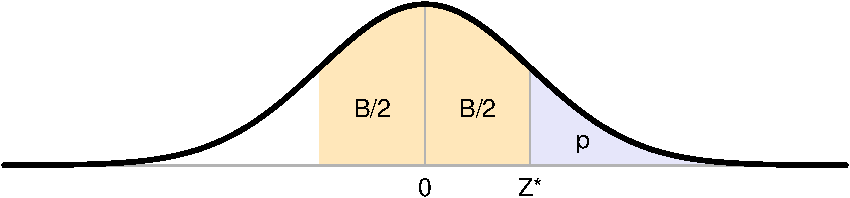
\includegraphics{QMS-EN_files/figure-latex/kritiekeZwaarden-hulpfiguur-1.pdf}

The critical value \(Z^*\) given below has a probability of \(p\) under \(H_0\), i.e.,
\(P(Z > Z^*|H_0)=p\) (the blue area),
and it has a probability of \(B\) to have a value in the interval \((-Z^*, +Z^*)\) (the yellow area).
The \(Z\) distribution is symmetrical around \(Z=0\), hence \(P(Z < -Z^*) = P(Z > Z^*)\).

\begin{center}\rule{0.5\linewidth}{0.5pt}\end{center}

The first table reports the critical boundary values \(Z^*\) for some frequently used probabilities of \(p\) and frequently used confidence intervals of \(B\):

\begin{tabular}{ccccccccc}
\toprule
p & 0.2 & 0.1 & 0.05 & 0.025 & 0.01 & 0.005 & 0.0025 & 0.001\\
\midrule
B & 60\% & 80\% & 90\% & 95\% & 98\% & 99\% & 99.5\% & 99.8\%\\
Z* & 0.8416 & 1.282 & 1.645 & 1.960 & 2.326 & 2.576 & 2.807 & 3.090\\
\bottomrule
\end{tabular}

\begin{center}\rule{0.5\linewidth}{0.5pt}\end{center}

The second table reports the probabilities \(p\) and confidence intervals \(B\) for some frequently used critical values of \(Z^*\):

\begin{tabular}{cccccccc}
\toprule
p & 0.3085 & 0.1587 & 0.0668 & 0.0228 & 0.0062 & 0.0013 & 0.0002\\
\midrule
B & 38.29\% & 68.27\% & 86.64\% & 95.45\% & 98.76\% & 99.73\% & 99.95\%\\
Z* & 0.5 & 1 & 1.5 & 2 & 2.5 & 3 & 3.5\\
\bottomrule
\end{tabular}

\hypertarget{app:criticaltvalues}{%
\chapter{\texorpdfstring{Critical values for \(t\)-distribution}{Critical values for t-distribution}}\label{app:criticaltvalues}}

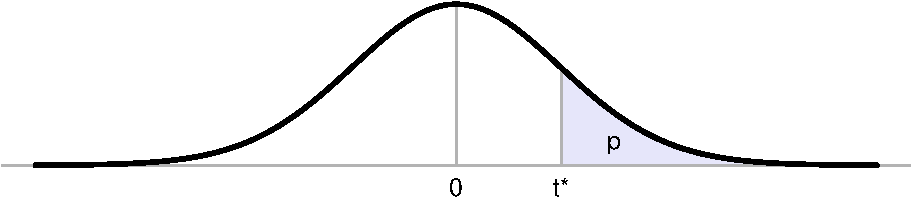
\includegraphics{QMS-EN_files/figure-latex/criticaltvalues-auxiliaryfigure-1.pdf}

The critical boundary value \(t^*\) given below has a critical probability \(p\)
under \(H_0\), i.e.~\(P(t \geq t^*|H_0)=p\), and has probability \(B\) of a
value between \((-t^*, +t^*)\). The \(t\)-distribution is symmetric around
\(t=0\), thus \(P(t < -t^*) = P(t > t^*)\).

The table below provides the critical boundary values \(t^*\) for much used critical probabilities \(p\) and
confidence intervals \(B\), for the degrees of freedom indicated in the first column.

\begin{tabular}{cccccccccc}
\toprule
 & p & 0.2 & 0.1 & 0.05 & 0.025 & 0.01 & 0.005 & 0.0025 & 0.001\\
\midrule
 & B & 60\% & 80\% & 90\% & 95\% & 98\% & 99\% & 99.5\% & 99.8\%\\
1 &  & 1.376 & 3.078 & 6.314 & 12.706 & 31.821 & 63.657 & 127.321 & 318.309\\
2 &  & 1.061 & 1.886 & 2.920 & 4.303 & 6.965 & 9.925 & 14.089 & 22.327\\
3 &  & 0.9785 & 1.638 & 2.353 & 3.182 & 4.541 & 5.841 & 7.453 & 10.215\\
4 &  & 0.941 & 1.533 & 2.132 & 2.776 & 3.747 & 4.604 & 5.598 & 7.173\\
\addlinespace
5 &  & 0.9195 & 1.476 & 2.015 & 2.571 & 3.365 & 4.032 & 4.773 & 5.893\\
6 &  & 0.9057 & 1.440 & 1.943 & 2.447 & 3.143 & 3.707 & 4.317 & 5.208\\
7 &  & 0.896 & 1.415 & 1.895 & 2.365 & 2.998 & 3.499 & 4.029 & 4.785\\
8 &  & 0.8889 & 1.397 & 1.860 & 2.306 & 2.896 & 3.355 & 3.833 & 4.501\\
9 &  & 0.8834 & 1.383 & 1.833 & 2.262 & 2.821 & 3.250 & 3.690 & 4.297\\
\addlinespace
10 &  & 0.8791 & 1.372 & 1.812 & 2.228 & 2.764 & 3.169 & 3.581 & 4.144\\
11 &  & 0.8755 & 1.363 & 1.796 & 2.201 & 2.718 & 3.106 & 3.497 & 4.025\\
12 &  & 0.8726 & 1.356 & 1.782 & 2.179 & 2.681 & 3.055 & 3.428 & 3.930\\
13 &  & 0.8702 & 1.350 & 1.771 & 2.160 & 2.650 & 3.012 & 3.372 & 3.852\\
14 &  & 0.8681 & 1.345 & 1.761 & 2.145 & 2.624 & 2.977 & 3.326 & 3.787\\
\addlinespace
15 &  & 0.8662 & 1.341 & 1.753 & 2.131 & 2.602 & 2.947 & 3.286 & 3.733\\
16 &  & 0.8647 & 1.337 & 1.746 & 2.120 & 2.583 & 2.921 & 3.252 & 3.686\\
17 &  & 0.8633 & 1.333 & 1.740 & 2.110 & 2.567 & 2.898 & 3.222 & 3.646\\
18 &  & 0.862 & 1.330 & 1.734 & 2.101 & 2.552 & 2.878 & 3.197 & 3.610\\
19 &  & 0.861 & 1.328 & 1.729 & 2.093 & 2.539 & 2.861 & 3.174 & 3.579\\
\addlinespace
20 &  & 0.860 & 1.325 & 1.725 & 2.086 & 2.528 & 2.845 & 3.153 & 3.552\\
21 &  & 0.8591 & 1.323 & 1.721 & 2.080 & 2.518 & 2.831 & 3.135 & 3.527\\
22 &  & 0.8583 & 1.321 & 1.717 & 2.074 & 2.508 & 2.819 & 3.119 & 3.505\\
23 &  & 0.8575 & 1.319 & 1.714 & 2.069 & 2.500 & 2.807 & 3.104 & 3.485\\
24 &  & 0.8569 & 1.318 & 1.711 & 2.064 & 2.492 & 2.797 & 3.091 & 3.467\\
\addlinespace
25 &  & 0.8562 & 1.316 & 1.708 & 2.060 & 2.485 & 2.787 & 3.078 & 3.450\\
30 &  & 0.8538 & 1.310 & 1.697 & 2.042 & 2.457 & 2.750 & 3.030 & 3.385\\
40 &  & 0.8507 & 1.303 & 1.684 & 2.021 & 2.423 & 2.704 & 2.971 & 3.307\\
50 &  & 0.8489 & 1.299 & 1.676 & 2.009 & 2.403 & 2.678 & 2.937 & 3.261\\
100 &  & 0.8452 & 1.290 & 1.660 & 1.984 & 2.364 & 2.626 & 2.871 & 3.174\\
\addlinespace
200 &  & 0.8434 & 1.286 & 1.653 & 1.972 & 2.345 & 2.601 & 2.839 & 3.131\\
400 &  & 0.8425 & 1.284 & 1.649 & 1.966 & 2.336 & 2.588 & 2.823 & 3.111\\
∞ &  & 0.8416 & 1.282 & 1.645 & 1.960 & 2.326 & 2.576 & 2.807 & 3.090\\
\bottomrule
\end{tabular}

\hypertarget{app:criticalchi2values}{%
\chapter{\texorpdfstring{Critical values for \(\chi^2\)-distribution}{Critical values for \textbackslash chi\^{}2-distribution}}\label{app:criticalchi2values}}

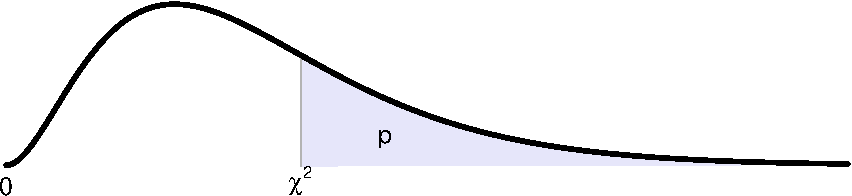
\includegraphics{QMS-EN_files/figure-latex/criticalchi2values-auxiliaryfigure-1.pdf}

The critical value \((\chi^2)^*\) given below has a critical probability \(p\) under
\(H_0\), i.e.~\(P(\chi^2 \geq (\chi^2)^*|H_0)=p\).

The table below provides the critical boundary values \((\chi^2)^*\) for much used critical probabilities \(p\), for the degrees of freedom indicated in the first column.

\begin{tabular}{cccccccccc}
\toprule
 & p & 0.2 & 0.1 & 0.05 & 0.025 & 0.01 & 0.005 & 0.0025 & 0.001\\
\midrule
1 &  & 1.64 & 2.71 & 3.84 & 5.02 & 6.63 & 7.88 & 9.14 & 10.83\\
2 &  & 3.22 & 4.61 & 5.99 & 7.38 & 9.21 & 10.60 & 11.98 & 13.82\\
3 &  & 4.64 & 6.25 & 7.81 & 9.35 & 11.34 & 12.84 & 14.32 & 16.27\\
4 &  & 5.99 & 7.78 & 9.49 & 11.14 & 13.28 & 14.86 & 16.42 & 18.47\\
5 &  & 7.29 & 9.24 & 11.07 & 12.83 & 15.09 & 16.75 & 18.39 & 20.52\\
\addlinespace
6 &  & 8.56 & 10.64 & 12.59 & 14.45 & 16.81 & 18.55 & 20.25 & 22.46\\
7 &  & 9.80 & 12.02 & 14.07 & 16.01 & 18.48 & 20.28 & 22.04 & 24.32\\
8 &  & 11.03 & 13.36 & 15.51 & 17.53 & 20.09 & 21.95 & 23.77 & 26.12\\
9 &  & 12.24 & 14.68 & 16.92 & 19.02 & 21.67 & 23.59 & 25.46 & 27.88\\
10 &  & 13.44 & 15.99 & 18.31 & 20.48 & 23.21 & 25.19 & 27.11 & 29.59\\
\addlinespace
11 &  & 14.63 & 17.28 & 19.68 & 21.92 & 24.72 & 26.76 & 28.73 & 31.26\\
12 &  & 15.81 & 18.55 & 21.03 & 23.34 & 26.22 & 28.30 & 30.32 & 32.91\\
13 &  & 16.98 & 19.81 & 22.36 & 24.74 & 27.69 & 29.82 & 31.88 & 34.53\\
14 &  & 18.15 & 21.06 & 23.68 & 26.12 & 29.14 & 31.32 & 33.43 & 36.12\\
15 &  & 19.31 & 22.31 & 25.00 & 27.49 & 30.58 & 32.80 & 34.95 & 37.70\\
\addlinespace
16 &  & 20.47 & 23.54 & 26.30 & 28.85 & 32.00 & 34.27 & 36.46 & 39.25\\
17 &  & 21.61 & 24.77 & 27.59 & 30.19 & 33.41 & 35.72 & 37.95 & 40.79\\
18 &  & 22.76 & 25.99 & 28.87 & 31.53 & 34.81 & 37.16 & 39.42 & 42.31\\
19 &  & 23.90 & 27.20 & 30.14 & 32.85 & 36.19 & 38.58 & 40.88 & 43.82\\
20 &  & 25.04 & 28.41 & 31.41 & 34.17 & 37.57 & 40.00 & 42.34 & 45.31\\
\addlinespace
21 &  & 26.17 & 29.62 & 32.67 & 35.48 & 38.93 & 41.40 & 43.78 & 46.80\\
22 &  & 27.30 & 30.81 & 33.92 & 36.78 & 40.29 & 42.80 & 45.20 & 48.27\\
23 &  & 28.43 & 32.01 & 35.17 & 38.08 & 41.64 & 44.18 & 46.62 & 49.73\\
24 &  & 29.55 & 33.20 & 36.42 & 39.36 & 42.98 & 45.56 & 48.03 & 51.18\\
25 &  & 30.68 & 34.38 & 37.65 & 40.65 & 44.31 & 46.93 & 49.44 & 52.62\\
\addlinespace
30 &  & 36.25 & 40.26 & 43.77 & 46.98 & 50.89 & 53.67 & 56.33 & 59.70\\
40 &  & 47.27 & 51.81 & 55.76 & 59.34 & 63.69 & 66.77 & 69.70 & 73.40\\
50 &  & 58.16 & 63.17 & 67.50 & 71.42 & 76.15 & 79.49 & 82.66 & 86.66\\
100 &  & 111.67 & 118.50 & 124.34 & 129.56 & 135.81 & 140.17 & 144.29 & 149.45\\
200 &  & 216.61 & 226.02 & 233.99 & 241.06 & 249.45 & 255.26 & 260.74 & 267.54\\
\addlinespace
400 &  & 423.59 & 436.65 & 447.63 & 457.31 & 468.72 & 476.61 & 483.99 & 493.13\\
\bottomrule
\end{tabular}

  \bibliography{book.bib,packages.bib,hhmhto.bib,pandoc.bib}

\end{document}
